 \documentclass[10pt]{book}

\usepackage{main/VotreFramabook}
\makeindex % dit à LaTeX de générer les index

\begin{document}
\selectlanguage{french}
\frontmatter % Intro (numéro de page en chiffres romains)
\thispagestyle{empty}
\null\vspace{\stretch{2}}
{\centering
	{\bfseries
		{\fontsize{28}{44}\selectfont\MakeTitre{}}\\
		{\fontsize{14}{44}\selectfont\version{}}\par
		{\fontsize{20.74}{22}\selectfont\soustitre}\par
		\vspace{\stretch{1}}
		{\fontsize{12}{36}\selectfont\MakeAuteur}\par
		\vspace{\stretch{1}}
		\begin{figure}[h]%
			\begin{center}%
				\leavevmode%
				\subfigure{%
					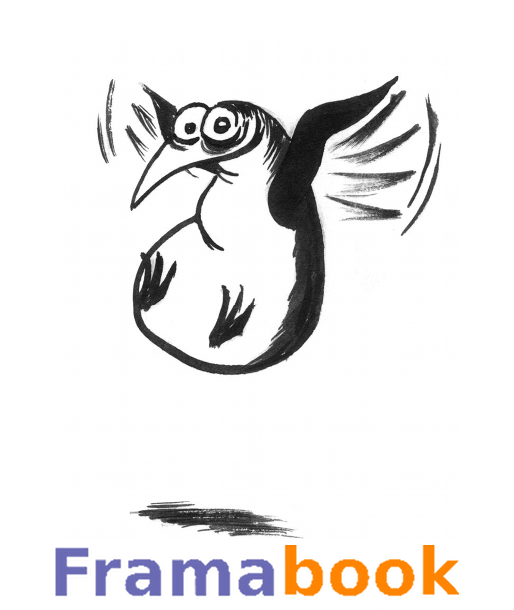
\includegraphics[width=4.06cm]{framabook/img/Framabook.png}}%
				\hspace{1cm}%
				\subfigure{%
					
\includegraphics[width=4.76cm]{framabook/img/ILV_P1.png}}%
			\end{center}%
		\end{figure}%
	}\newpage\thispagestyle{empty}
	{\bfseries\fontsize{14}{16}\selectfont{}ÉDITIONS}\par
	\begin{figure}[h]
		\begin{center}
			
\includegraphics[width=4.76cm]{framabook/img/ILV_P2.png}
		\end{center}
	\end{figure}
	{\fontsize{14}{16}\selectfont{}Immeuble ACCET\\
														4, place de la Pergola\\
														95021 Cergy-Pontoise Cedex }\par
	\vspace{\stretch{3}}
	{\fontsize{12}{14}\selectfont{}Ce livre et l'illustration en couverture sont publiés sous la licence libre\\\textbf{Creative Commons-BY-SA} :\\\url{http://creativecommons.org/licenses/by-sa/2.0/fr}\par}
}
{\setlength{\parskip}{1.5\baselineskip}
	\textbf{BY : Paternité.} Vous devez citer le nom de l'auteur original.\par
	\textbf{SA : Partage des Conditions Initiales à l'Identique.} Si vous modifiez, transformez ou adaptez cette création, vous n'avez le droit de distribuer la création qui en résulte sous un contrat identique à celui-ci.\\
	En outre, à chaque réutilisation ou distribution, vous devez faire apparaître clairement les conditions contractuelles de mise à disposition de cette création. Chacune de ces conditions peut être levée si vous obtenez l'autorisation du titulaire des droits.\par
}
\vspace{\stretch{2}}
{\centering\setlength{\parskip}{2\baselineskip}
	In Libro Veritas, \anneedepot{}, ISBN : \isbn\par
	Dépôt légal : \datedepot\par
}
\vspace{\stretch{4}}

\ifversionpdf
    \thispagestyle{empty}
\null\vspace{\stretch{2}}
{\centering\fontsize{14}{16}\selectfont{}Simple Comme Ubuntu est un livre libre du projet framabook.\\
Vous pouvez vous en procurer une version papier sur\\\url{http://framabook.org/ubuntu.html}}\par
{\fontsize{12}{14}\selectfont{}Description du projet \textbf{Framabook}. Également disponible sur \url{http://framabook.org} :\par
\textbf{Un projet original}\\
Se démarquant de l'édition classique, les framabooks sont dits «~livres libres~» parce qu'ils sont placés sous une licence qui permet au lecteur de disposer des mêmes libertés qu'un utilisateur de logiciels libres.\\
Nous incitons à commander les livres pour soutenir le projet mais, quel que soit votre choix, libre à vous, en accord avec la licence, d'utiliser, copier, modifer et distribuer leurs versions numériques, ou tout simplement de tester avant d'acheter ;-)\par
\textbf{Un projet culturel}\\
De par leur licence libre, les framabooks s'inscrivent dans cette culture des biens communs qui, à l'instar de Wikipédia, favorise la création, le partage, la diffusion et l'appropriation collective de la connaissance.\par
\textbf{Un projet économique}\\
Nous aimerions montrer que, contrairement à certaines idées reçues, proposer des livres sous licence libre n'est pas un frein à la réussite commerciale du projet.\\
Le «~pari du livre libre~» c'est non seulement réussir à créer une collection de qualité mais c'est aussi arriver à rendre le modèle économiquement viable.\\
C'est important pour les auteurs qui n'ont pas ménagé leurs temps et leurs efforts pour nous offrir des ouvrages d'excellentes tenues. C'est important pout notre partenaire éditeur qui, partie prenante de l'aventure, a tout fait pour tirer les prix vers le bas sans sacrifier à la qualité d'impression. C'est important enfin pour le projet en lui-même et peut-être aussi par extension pour tout projet qui hésiterait à adopter un tel modèle jugé a priori à risque.\par
\textbf{Un projet à soutenir}\\
Si notre approche particulière rencontre votre adhésion, nous vous invitons à nous soutenir en liant ce site, en évoquant ce projet autour de vous mais aussi et surtout en achetant la déclinaison physique des framabooks, à savoir les livres édités par InLibroVeritas.\\
Un achat susceptible de vous être directement utile dans la découverte et l'usage d'un logiciel libre donné, mais un achat que vous pouvez également offrir en cadeau à vos proches, faisant alors d'une pierre deux coups : diffuser du logiciel libre et nous aider dans notre action.\\
Ajoutons enfin que la majorité des auteurs ont choisi de reverser un pourcentage de leurs bénéfices aux équipes et associations du logiciel libre dont traite leur ouvrage, illustrant ainsi le fameux cercle vertueux de la culture libre.\par
\textbf{Un projet en mouvement}\\
Notre objectif est de faire connaître et diffuser le logiciel libre au plus large public. Nous n'ignorons pas que cela implique souvent de rompre avec certaines habitudes acquises avec d'autres logiciels non libres.\\
Quitter la messagerie Outlook Express, la suite bureautique MS Office ou Windows Vista pour les alternatives libres Thunderbird, OpenOffice.org et GNU/Linux Ubuntu n'est pas toujours chose aisée.\\
Les framabooks, accessibles, illustrés et détaillés, facilitent de telles migrations et participent de ce mouvement de bascule du logiciel propriétaire vers le logiciel libre.\par
\newpage
\textbf{Un projet réactif}\\
Les caractéristiques des framabooks (collaboration, licences libres, tirages limités) permettent de suivre au plus près les évolutions des logiciels et d'offrir au lecteur un contenu rapidement réactualisé.\\
C'est ainsi que, par des auteurs parfois différents de ceux d'origine, les deux premiers volumes sur Thunderbird et Ubuntu ont été mis à jour et réédités peu de temps après les changements de version des logiciels en question.\par
\textbf{Un projet en quête d'auteurs}\\
Vous souhaitez nous rejoindre et écrire un futur framabook accompagné par notre fine équipe ? Il suffit d'accepter le principe des licences libres et d'être motivé par un travail passionnant mais de longue haleine. Vous trouverez de plus amples informations sur notre forum mais vous pouvez aussi nous contacter directement.\\
Pour vous donner un ordre d'idées sachez qu'en octobre 2008 nous totalisions près de quatre mille exemplaires vendus.\\
Exemples de poste à pourvoir : Inkscape, Firefox, Scribus, Freemind, Amarok, Drupal, Mediawiki, etc.\par
\textbf{Un projet matérialisé par InLibroVeritas}\\
Les framabooks seraient restés virtuels sans le concours de Mathieu Pasquini, fondateur de la maison d'édition pas comme les autres InLibroVeritas.\\
Parmi les nombreux autres livres disponibles chez l'éditeur on notera l'ouvrage collectif Tribune Libre, ténors de l'informatique libre, le dernier Perline (avec Thierry Noisette) Vote électronique : les boîtes noires de la démocratie, le très actuel Internet et Création de Philippe Aigrain, L'urgence de la métamorphose de Laurence Baranski et Jacques Robin ou encore la réédition du Hold-Up planétaire, la face cachée de Microsoft de Roberto Di Cosmo.\par
\textbf{Un projet Framasoft}\\
S'appuyant sur une association éponyme, Framasoft est un réseau de sites web collaboratifs à géométrie variable dont le dénominateur commun est le logiciel libre et son état d'esprit. Il vise à faire connaitre et diffuser le logiciel libre au plus large public.\\
Lieu d'informations, d'actualités, d'échanges et de projets, Framasoft, de par la diversité et le dynamisme de son réseau, est aujourd'hui l'une des portes d'entrée francophones du logiciel libre. Sa communauté accompagne ceux qui souhaitent substituer leurs logiciels propriétaires par des logiciels libres. Elle attache une attention toute particulière au processus de migration du système d'exploitation Microsoft Windows, XP ou Vista, vers GNU/Linux.\\
Parmi les nombreuses ressources du réseau on trouve un annuaire de plus d'un millier de logiciels libres, une clé USB dite Framakey spécialisée dans les applications portables libres Windows, un forum où le néophyte est le bienvenu et un blog qui constate au quotidien que le logiciel libre est en train de libérer bien plus que du simple code et Framabook est bien placé pour en témoigner !
}

\fi
\sommaire
\TitreIntro{Préface}
Quand je croise quelqu'un qui n'a pas encore vu une série comme Les Soprano ou Battlestar Gallactica, au lieu de hurler au scandale et à l'inculture crasse (je pourrais, notez), je ne peux pas m'empêcher de penser «~petit(e) veinard(e)~». Parce que le plaisir de la découverte ne m'est plus accessible. Je peux les revoir, certes, mais il m'est difficile aujourd'hui de m'extasier devant tel retournement ou d'être assommé par telle révélation sur un personnage. La première fois n'arrive qu'une fois. C'est bien dommage.\par
Donc si vous être en train de lire cet (excellent) ouvrage parce que vous avez décidé de franchir le pas, de partir à la découverte d'Ubuntu\ldots{} petits veinards. Je suis un peu jaloux. Comme pour une série ou un film, je m'en voudrais de dévoiler dès maintenant toutes les petites découvertes qui vous attendent. Je ne vais pas «~spoiler~» Ubuntu, rassurez-vous, mais les premiers pas dans ce système libre vous réservent quelques bonnes surprises, et quelques retournements de situation sympathiques. Mais je ne vais pas jouer au vieux sage qui regarde d'un œil malicieux le jeune disciple qui a décidé de se lancer sur la voie du shaolin, je n'en suis moi-même qu'à mes débuts. Un peu plus de trois mois à l'heure où j'écris ces lignes que j'utilise quotidiennement un ordinateur portable sous Ubuntu. Et mises à part quelques mésaventures sans grande importance que j'ai raconté ailleurs\NotePage{Le journal d'un novice sur Ecrans.fr, \url{http://www.ecrans.fr/+-le-journal-d-un-novice-+.html?page=journal}}, tout roule parfaitement bien. J'ai même réussi à faire fonctionner ma souris bluetooth, c'est dire !\par
Ces quelques mois de pratique ne font pas de moi un gourou d'Ubuntu, loin s'en faut. Et je n'ai pas la prétention de le devenir un jour. Mais ma petite expérience m'a appris quelques petits trucs que je me permets de retranscrire sous la forme de petites règles. Rien d'impératif, comme toutes les règles, elles existent aussi pour être transgressées.\par
\begin{description}
\item[Règle N°1 :] La découverte d'Ubuntu, c'est un jeu. Non pas un jeu d'enfant (quoique\ldots{}), mais un parcours ludique qu'il faut aborder l'esprit ouvert. Il y aura sans doute des obstacles, des petits («~hum\ldots{} dois-je cliquer sur «~Appliquer~» ou sur «~Annuler~») et des plus grands («~comment puis-je faire pour utiliser cette imprimante qui date du 20e siècle ?~»), mais ils ne sont pratiquement jamais insurmontables. Et si on prend la chose du côté ludique, on s'amuse plus qu'on ne rouspète. En plus, pour reprendre une expression du jeu vidéo, si la difficulté devient trop grande, les soluces sont sur Internet.
\item[Règle N°2 :] Installer Ubuntu, c'est un choix. Faire le choix de son système d'exploitation est sans doute une nouveauté pour vous. En tout cas, ça l'a été pour moi. Quinze ans sous Windows avant de franchir le pas. C'est la seule fois où, à l'achat d'un ordinateur, je me suis demandé quel système j'allais prendre. Jusqu'ici, l'alternative consistait à acheter une machine Apple livrée avec son propre système, ou un PC plus classique et donc Windows. Sans avoir de choix, car on ne se pose même pas la question. Pour passer à Linux, il faut que cette question existe. Avec ce choix, il n'y a aucune obligation en absolu. Vous l'avez peut-être fait tout simplement à cause de la gratuité du système. Mais même dans ce cas, je ne saurais trop vous conseiller de vous renseigner sur ce qui a permis que vous puissiez le faire. Logiciel libre, GNU, GPL, open-source, l'histoire de ce dernier quart de siècle est passionnante. Aussi, prendre conscience de la somme de travail qui a permis à Ubuntu et à d'autres systèmes et logiciels de voir le jour permet de relativiser ses petits soucis de souris Bluetooth (non, je ne fais pas une fixation).
\item[Règle N°3 :] Vous n'êtes pas seuls. C'est sans doute un des points les plus extraordinaires de Linux et donc d'Ubuntu : la serviabilité de ses utilisateurs. Si vous avez un problème, non seulement vous pouvez être sûr que quelqu'un l'a déjà eu et que la réponse se trouve dans un des nombreux forums de discussions et blogs existant, mais si par le plus grand des hasards ce n'était pas le cas, il suffit de poser la question pour qu'un habitué vienne à votre secours. Bon, d'accord, parfois, ils sont un peu bizarres et ils parlent un langage qui peut paraître étrange, mais croyez-moi, ils feront tout pour vous aider. Pourquoi ? Peut-être à cause des deux premières règles que j'ai énoncé. Et vous verrez, d'ici quelques mois, vous finirez peut-être par aider un débutant à se dépatouiller. C'est toujours très gratifiant.
\item[Règle N°4 :] Ubuntu, ce n'est qu'un système d'exploitation. Rien de plus. Je sais, c'est déjà énorme, mais quand vous allumez votre ordinateur, ce n'est pas pour admirer l'écran de lancement. Enfin, on peut, mais ça devient un peu lassant à la longue. Le but d'un système d'exploitation, c'est de se faire oublier. D'ici quelques semaines (quelques jours, même), vous allumerez votre ordinateur, vous lancerez votre navigateur web, vous retoucherez vos photos, vous écrirez des textes sans même vous soucier de ce qui fait tourner tout ça. Aujourd'hui, des milliers de personnes, moi le premier, utilisent Ubuntu pour une utilisation courante (Internet, bureautique, images, etc.) sans rencontrer le moindre problème. Aucune raison qu'il en soit autrement dans votre cas.
\item[Règle N°5 :] Il est interdit de parler du Fight Club. Euh\ldots{} Non, ça, c'est une autre histoire.
\end{description}
Mais c'est vrai, faire ses premiers pas sur un nouveau système d'exploitation, c'est parfois un peu intimidant. C'est un peu comme partir en voyage dans un pays qu'on ne connaît pas et dont on ne parle pas la langue (mais on a vu des photos, il paraît que c'est très joli!). C'est là que Simple comme Ubuntu entre en jeu. Le livre de \Personne{Didier}{Roche}, c'est un peu le Guide du Routard d'Ubuntu. On y trouve un descriptif complet de l'endroit, des itinéraires conseillés, des bonnes adresses, les bons plans et les lieux à visiter (ne ratez pas le gestionnaire de paquets, c'est magnifique). En suivant ses indications, difficile de se perdre. Et vous êtes sûr de ne rien rater d'important. Et puis, peut-être, après avoir écorné les pages, souligné les petits trucs, cerclé les points importants (rien que pour ça, achetez le livre, en pdf, c'est plus dur), vous vous sentirez à l'aise pour partir à l'aventure sur les chemins de traverse d'Ubuntu.\par
Mais n'allons pas trop vite. Chaque chose en son temps. Je ne veux pas vous retarder, la séance va commencer. Prenez vos places, installez-vous confortablement.\par
Il était une fois un bouquetin intrépide\ldots{}\par
{\vspace{\stretch{1}}{\centering%
		{\fontsize{12}{36}\selectfont \Personne{Erwan}{CARIO}}\par Journaliste sur Écrans.fr\par\vspace{\stretch{4}}}%

\TitreIntro{Préface de l'auteur}
Beaucoup d'utilisateurs sont mécontents des services offerts par leur \RefGlossaire{Système}{OS}{Système d'exploitation}{système d'exploitation} actuel : bugs, plantages fréquents, travail effacé ou perdu et formatages récurrents. Ils entendent alors parler de Linux, mais dans leur esprit, ce dernier reste un \RefGlossaire{Système}{Système d'exploitation}{OS}{OS} complexe, où tout doit se faire «~à la main~». De plus, certains utilisateurs reviennent sous Windows après un court passage à Linux en expliquant que «~c'est compliqué, c'est vraiment un \RefGlossaire{Système}{OS}{Système d'exploitation}{système d'exploitation} qui n'est pas fait pour les utilisateurs mais pour les programmeurs~» (quand ils ne disent pas «~programmateurs~» ! :-)), ce qui ajoute encore plus à cette idée largement répandue d'inaccessible complexité.\par
Alors, GNU/Linux est-il réellement un \RefGlossaire{Système}{OS}{Système d'exploitation}{système d'exploitation} élitiste ? Êtes-vous vraiment obligés de passer des heures et des heures pour configurer correctement votre \RefGlossaire{Système}{OS}{Système d'exploitation}{système d'exploitation}, installer un logiciel et autres opérations qui, je le vois déjà, ne vous réjouissent pas ?\par
Le principal frein concernant ce point est assurément la multitude des documentations existantes sur l'\RefGlossaire{-}{L'Internet}{Internet}{Internet}, ce qui peut faire perdre de vue à l'utilisateur débutant les clefs vraiment essentielles à une utilisation quotidienne. Un deuxième problème, indépendant de Linux lui-même, est que «~GNU/Linux n'est pas Windows~» : l'attachement du nouveau venu à ses habitudes «~fenêtresques~» est, en effet, assez tenace. Je prendrai comme exemple le téléchargement d'un programme depuis l'\RefGlossaire{-}{L'Internet}{Internet}{Internet}. On va sur un site de gratuiciels le plus souvent, et on prend un fichier archive (souvent un .zip). On s'attend à trouver un fichier .exe à l'intérieur de ce dernier et à double-cliquer dessus pour l'installer\NotePage{Puis d'effectuer «~suivant~», «~suivant~», «~suivant~», sans lire la licence, évidemment\ldots{}}. Le nouvel utilisateur linuxien va essayer de reproduire le même comportement sur son nouvel OS : il va télécharger une archive\NotePage{Le plus souvent .tar.gz} sur un site, mais ne va pas trouver son «~si confortable~» setup.exe ! Il cherche sur un forum et on lui parle alors de fichier «~source~» à «~compiler~». Et voilà que des utilisateurs, venant d'installer Linux pour la première fois, essaient, dans la foulée, de compiler un logiciel. Par la force des choses, ces débutants vont rapidement arriver au constat que GNU/Linux n'est vraiment pas «~user-friendly~».\par
Pourquoi cet essai systématique de mimétisme ? La plus simple des réponses trouve très certainement son explication dans l'existence d'un facteur «~confort\NotePage{Et sûrement de facilité !}~», car lorsque l'on maîtrise un \RefGlossaire{Système}{OS}{Système d'exploitation}{système d'exploitation}, on s'attend à retrouver ses repères, puisque «~on nous a appris comme cela~». Et si on peine pour une chose aussi bête que l'installation d'un logiciel, on se dit que le système n'est pas adapté. Cependant, si vous vous rappelez vos premiers pas en informatique, rien n'a été inné : c'est vous qui vous êtes adapté à votre \RefGlossaire{Système}{OS}{Système d'exploitation}{système d'exploitation} et en avez pris les -- parfois mauvaises -- habitudes. Ne vous attendez pas à maîtriser Linux en une journée ; est-ce le temps qu'il vous a fallu pour maîtriser votre \RefGlossaire{Système}{OS}{Système d'exploitation}{système d'exploitation} actuel ?\par
Il faut donc «~penser autrement~» car vous êtes sur un \RefGlossaire{Système}{OS}{Système d'exploitation}{système d'exploitation} différent, dont la philosophie n'est pas de copier le fonctionnement d'autres systèmes, mais d'en offrir une alternative avec d'autres modes de pensée\NotePage{Vous verrez par exemple au chapitre 4 qu'installer une application est vraiment une sinécure sous Ubuntu.}. Mais pour cela, me direz-vous, il faut que l'on vous aide et vous montre la voie pour être efficace le plus rapidement possible. C'est en ce sens que ce livre a été écrit et vous verrez que Linux n'est pas plus compliqué que Windows\NotePage{Sur certains points, il est même beaucoup plus simple !}, mais correspond à une logique «~différente~». Les mauvaises migrations -- les personnes revenues à Windows -- sont principalement des individus autodidactes qui maîtrisaient très bien leur \RefGlossaire{Système}{OS}{Système d'exploitation}{système d'exploitation}, mais étaient totalement incapables de s'adapter à Linux car elles en attendaient exactement le même comportement. Bouleverser ses habitudes ne vient pas sans heurts, en effet, mais lorsque l'on y arrive, quelle satisfaction !\par
Je peux vous certifier que j'utilise quotidiennement GNU/Linux. Eh bien, je peine parfois énormément sous Windows à effectuer une opération pourtant simple, alors que je pense avoir bien maîtrisé ce \RefGlossaire{Système}{OS}{Système d'exploitation}{système d'exploitation} à une époque. Selon moi, la distribution Ubuntu, que je suis, à ma grande satisfaction, depuis sa création -- lorsque la première mouture n'était pas encore véritablement sortie -- jusqu'à aujourd'hui, apporte vraiment une alternative simple à Windows. Bien évidemment, ce jugement n'engage que moi et, bien qu'il existe de très nombreuses distributions GNU/Linux ou encore Mac OS, les moyens mis en œuvre dans celle-ci font preuve d'un véritable professionnalisme. Vous l'aurez compris, Ubuntu est clairement orientée vers les utilisateurs et les entreprises.\par
À partir du travail d'un blogueur de la communauté d'Ubuntu, «~Yekcim~», qui décrivait l'installation de cet \RefGlossaire{Système}{OS}{Système d'exploitation}{OS} et le listing de quelques programmes et jeux, j'ai pleinement pris conscience de la nécessité d'une documentation française aisément identifiable qui guide les utilisateurs débutants dans leurs premiers pas sous ce \RefGlossaire{Système}{OS}{Système d'exploitation}{système d'exploitation}. J'ai donc repris son ensemble de billets\NotePage{La licence le permettait et est la même que celle de ce livre} qui s'étendait alors sur une quinzaine de pages pour réaliser une documentation très expurgée, qui devait rester la plus succincte possible. Puis, de fil en aiguille, je me suis pris au jeu en ajoutant logiciels, jeux, astuces d'utilisation, précisions sur le système\ldots{}\par
La documentation a connu, à ma grande surprise, un vrai succès sur le forum de la communauté francophone d'Ubuntu et de plus en plus de personnes l'ont conseillée aux débutants. De plus, elle a été adaptée par des utilisateurs vers des distributions comme Kubuntu et Xubuntu ! J'ai ensuite été contacté par Framasoft qui m'a présenté son projet de collection de livres sous \AddIndex{Philosophie}{-}{Licence Libre}{licence libre}. J'y ai donc pris part et cela m'a motivé pour améliorer et finaliser ce qui n'était encore, à l'époque, qu'une simple documentation en ce véritable livre que vous tenez entre vos mains.\par
À la sortie de la version Feisty Fawn d'Ubuntu, une mise à jour était nécessaire aux vues des nouveautés apportées par cette version. J'apprenais, pour le milieu professionnel, les rudiments de \LaTeX{}. J'ai alors tout naturellement proposé à Framabook que l'on uniformise les présentations des différents livres en préparation en passant à ce format, proposition ayant été couronnée de succès après débats internes et externes. Une grande refonte a donc été effectuée afin de changer la présentation, et de la rendre plus conforme aux standards du livre. La version que vous tenez entre les mains est le résultat de cette présentation en \LaTeX{}, mise à jour et adaptée à la version Maverick Meerkat (10.10).\par
Je tiens enfin à souligner que cette documentation n'est vraiment pas une confrontation «~GNU/Linux versus Windows~» en faisant tout pour enjoliver le premier et détruire le second, bien que quelques piques et réécritures orthographiques intentionnelles je l'admets, existent au cours des divers chapitres. Je vous présente un nouveau \RefGlossaire{Système}{OS}{Système d'exploitation}{système d'exploitation} et vous explique ce qui le différencie de Windows.\par
Croyant à l'expression «~Talk to the mind, not to the brain~»\NotePage{Parlez à l'esprit et non au cerveau}, ce livre est écrit dans un style plutôt «~libre~» -- décidément ! -- afin de ne pas rendre le résultat trop indigeste. J'espère ainsi que chaque chapitre vous donnera un peu plus envie d'aller de l'avant.\par

\TitreIntro{Notre public}
Ce livre s'adresse tout particulièrement aux utilisateurs de Windows désireux de passer sous GNU/Linux. De plus, il peut aussi présenter la distribution Ubuntu à des utilisateurs d'autres distributions Linux, et également aux possesseurs de systèmes Mac OS X. De nombreuses captures d'écran jalonnent ce livre pour que, je l'espère, vous ne soyez jamais perdu.\par
Ce livre ne fera pas de vous un maître incontesté de GNU/Linux\NotePage{Bien que lorsque vous arriverez à l'avant-dernier chapitre, vous commencerez à en maîtriser les ficelles !}, mais vous guidera dans vos premiers pas sous Ubuntu pour que vous sachiez l'installer, ajouter de nouveaux logiciels et jeux, et l'utiliser quotidiennement. De plus, il constitue une bonne introduction à une compréhension plus avancée du système d'exploitation et vous donnera les clefs pour aller plus loin, si vous le désirez\ldots{}\par

\TitreIntro{Le plan de cet ouvrage}
Ce livre se veut comme une progression pas à pas dans la découverte de votre nouveau système d'exploitation ; chaque chapitre marque une étape importante de ce déroulement. Je conseille donc à tout nouvel apprenti de lire ce livre dans l'ordre, sans faire de grandes coupes franches afin de comprendre sans trop d'efforts les étapes suivantes.\par
\begin{DescriptionChapitres}
\item [Chapitre 1] Ce chapitre comprend une courte introduction au Logiciel Libre et, en particulier à GNU/Linux, en insistant sur la philosophie et les différences avec le logiciel propriétaire. Vous y trouverez également les réponses à quelques questions d'ordre général.
\item [Chapitre 2] On y découvre comment obtenir Ubuntu, l'essayer sans risquer de perdre des données et enfin, se lancer dans une séance d'installation.
\item [Chapitre 3] Le chapitre 3 explique les notions de base à connaître lorsque l'on «~plonge~» dans GNU/Linux ! Il vous guidera aussi dans la découverte de votre nouvel environnement de travail.
\item [Chapitre 4] Vous trouverez dans ce chapitre une explication sur l'installation d'un réseau (et de l'Internet) sur votre nouveau système d'exploitation. Vous serez également initié à la bonne manière de procéder à l'installation de logiciels et de jeux à partir des outils mis en place par Ubuntu.
\item [Chapitre 5] Il présente les derniers points et «~réglages~» à effectuer pour rendre votre système utilisable quotidiennement, avec, par exemple, le téléchargement des codecs vidéos, la liaison de Firefox avec des composants tels que Flash et Java\ldots{}
\item [Chapitre 6] Voici sûrement le chapitre qui vous intéressera le plus : il décrit les trucs et astuces qui permettent de gagner du temps et d'utiliser plus intelligemment son environnement de travail. Vous y trouverez également quelques conseils sur l'utilisation de Firefox.
\item [Chapitre 7] Le chapitre 7 traite des derniers points matériels qui peuvent poser problème comme la configuration de l'imprimante. Il vous guide également à l'aide d'un exemple dans l'utilisation d'un scanner, du bureau 3D et d'une configuration de démarrage.
\item [Chapitre 8] Vous y trouverez une liste de logiciels classés par catégorie permettant rapidement de repérer et choisir un logiciel à installer pour tel ou tel type d'utilisation.
\item [Chapitre 9] Dans le chapitre 9, vous découvrirez un nombre impressionnant de jeux disponibles sous GNU/Linux. Ceux-ci, classés par genre, contiennent les instructions complètes d'installation.
\item [Chapitre 10] Le chapitre 10 est un aparté qui peut vous emmener plus loin dans la connaissance et la compréhension de votre système d'exploitation. Bonne nouvelle, celui-ci est optionnel !
\item [Chapitre 11] Conclusion de cet ouvrage, ce chapitre vous permettra de savoir où chercher de l'aide, des informations et comment s'investir dans le monde du Libre.
%il présentera notamment des notions telles que «~Pourquoi le libre~» et vous amènera très certainement à voir les enjeux présents et la culture libre sous un angle différent.
\item [Glossaire] Le glossaire vous permettra d'accéder rapidement à la définition de certains termes réservés au monde de l'informatique.
\item [Index] Un index, très pratique, vous renverra, à l'aide d'une recherche par catégorie et mots-clefs, aux pages du livre correspondantes.
\item [Table des matières] Une table des matières complète, recensant toutes les sections de cet ouvrage, clôt ce livre.
\end{DescriptionChapitres}

\TitreIntro{Conventions utilisées dans ce livre}
\label{RefExemple}
Pour permettre une lecture et un repérage plus simples de ce livre, voici les conventions que l'on s'est fixées :\par
Un renvoi vers une autre partie du livre est indiqué de la sorte : cf. page \pageref{RefExemple}.\par
Les notes de bas de page sont représentées ainsi\NotePage{Je ne sais pas si vous avez remarqué, mais la référence précédente était une référence auto-récursive ;)}.\par
La navigation entre un menu et un sous-menu est séparée par cette flèche \FlecheDroite très esthétique !\par
Des chemins vers des fichiers et des dossiers sont présentés de cette manière : \Chemin{vers/l/infini/et/au/delà}.\par
Une touche du clavier est mise en évidence comme la touche \Touche{Entrée}. Un signe + est ajouté si vous devez presser simultanément plusieurs touches.\par
Un élément décrit dans le glossaire$^*$ bénéficie également d'une mise en évidence particulière.\par
Les commandes à entrer dans un terminal sont mises en valeur de cette manière : \Commande{Une ligne de commande}. Elles sont -- le plus souvent -- à saisir sur une seule ligne, la mise en page d'un livre ne permettant pas, la plupart du temps, de l'écrire ainsi.\par
Une note plus longue -- et plus importante -- est indiquée de la sorte : \begin{nota}Cette note devrait normalement apporter des précisions supplémentaires au sujet précédent. Cependant, ces informations ne sont pas non plus capitales.\end{nota}\par
Les notes plus importantes, quant à elles, sont représentées comme ceci : \begin{attention}Ceci est une note importante, elle essaie d'attirer votre attention sur un point précis à ne pas négliger afin que la suite des opérations indiquées dans le livre se déroule sans heurts.\end{attention}\par
Les lignes de code représentent la sortie du terminal. Cette présentation est également utilisée lorsqu'un grand nombre d'éléments sont à entrer dans un fichier : \Code{\# Ceci est un commentaire dans un fichier de configuration\\
\# Le plus souvent, ce dernier est présent sur plusieurs lignes}\par
Quelques citations jalonnent ce livre et sont représentées de la sorte :\par
\begin{citationlongue}{Pythagore a dit}
Les amis sont des compagnons de voyage, qui nous aident à avancer sur le chemin d'une vie plus heureuse.
\end{citationlongue}\par
Ce livre existe également dans un format électronique où les adresses internet comme celle de framabook -- \url{http://www.framabook.org} -- sont des hyperliens, et les liens internes comme les notes de bas de page sont également actifs.\par
\vspace{\stretch{1}}
Je tiens enfin à rappeler que les adresses Internet sont malheureusement par nature, appelées à varier : un lien, valide lors de l'écriture de ce livre, peut donc devenir invalide.
\vspace{\stretch{10}}

\TitreIntro{Remerciements}
\begin{Remerciements}
Je tiens à remercier tout d'abord les développeurs de logiciels libres et leurs contributeurs, en particulier ceux de la Fondation Ubuntu, pour leur sens de l'intérêt général, du partage, de l'entraide et de l'innovation. Merci également à \Personne{Mark}{Shuttleworth} pour son dynamisme et sa communication sur les objectifs de sa distribution.\par
Je n'oublie pas non plus mes parents qui m'ont permis d'accéder à l'outil informatique dès mon plus jeune âge. Je tiens également à saluer \Personne{Vanessa et Dimitri}{Perrin} pour leur soutien et pour avoir rendu mon séjour en Irlande agréable.\par
Cette tâche a été effectuée à partir de l'énorme travail d'\Personne{Anthony}{Carré}\NotePage{\url{http://yeknan.free.fr}}, initialement adapté au format imprimable par jokx\NotePage{\url{http://wenux.net}}, ce qui m'a plus que motivé à la rédaction de ce document. J'aimerais aussi inclure dans les remerciements les trois co-auteurs \Personne{Julien}{Rottenberg}, \Personne{Guillaume}{Ludwig} et \Personne{Joseph}{Massot}. Leur livre n'a malheureusement jamais pu sortir. Les parties de l'installation de l'imprimante et du scanner sont (quasi) intégralement basées sur leur travail, ainsi que quelques ajouts dans la description des menus.\par
Cette documentation est également «~librement~» inspirée de quelques billets du blog de \Personne{David}{Szerman}\NotePage{\url{http://www.szdavid.com}}, de \Personne{Jean-Baptiste}{Hétier}\NotePage{\url{http://www.think-underground.com}}, de Asher\NotePage{\url{http://asher256.tuxfamily.org}} -- par son travail sur son dépôt -- de  \Personne{Grégory}{Gutierez}\NotePage{\url{http://petitlinux.greguti.com}}, sans oublier le wiki de notre chère communauté francophone\NotePage{\url{http://doc.ubuntu-fr.org}} et sa mailing-list toujours aussi accueillante. L'excellent site \url{http://www.whylinuxisbetter.net} a également été une source d'inspiration importante, merci à  \Personne{Manu}{Cornet}, son créateur.\par
Ce livre réalisé en \LaTeX{} n'aurait jamais été possible sans l'excellent guide «~Tout ce que vous avez voulu toujours savoir sur \LaTeX{} sans jamais oser le demander~» de \Personne{Vincent}{Lozano}, autre livre de la collection Framabook. Surveillez \url{http://www.framabook.org} !\par
Un grand merci également à toutes les personnes qui ont apporté leur pierre à l'édifice par le biais du forum, notamment \Personne{Raphaël}{Bourven} pour son énorme travail de relecture\NotePage{Et il a même re-signé pour les nouvelles versions, le bougre !} et les nombreuses corrections apportées par la communauté d'Ubuntu-fr dont \Personne{Fabrice}{Braillon}, \Personne{Franck}{Chadel}, \Personne{Quentin}{Bricard} et \Personne{Claude}{Crozet}, ainsi que par le contributeur très productif qui sait se lancer dans un sprint final éhonté\NotePage{Il ne sait que trop bien ce que signifie «~On boucle demain midi !~» ;-)}, à de multiples reprises : \Personne{Bruno}{Le Clainche}.\par
Cette version a également bénéficié du groupe de lecture de Framabook par les participations actives de \Personne{Barbara}{Bourdelles}, \Personne{Yann}{GUERON} \Personne{Raymond}{Rochedieu}, \Personne{Antoine}{Blanche} et Metta Om.\par
Enfin, je témoigne ma gratitude à \Personne{Alexis}{Kauffmann}\NotePage{\url{http://framablog.org}}, fondateur de Framasoft\NotePage{\url{http://www.framasoft.net}} pour avoir cru qu'il était possible de transformer ma documentation en un livre, qui, je l'espère, vous plaira, ainsi qu'à \Personne{Mathieu}{Pasquini}\NotePage{\url{http://www.inlibroveritas.net}}, mon éditeur, pour son soutien même dans les moments les plus difficiles.\par
Ce livre essaie de respecter au maximum les règles de la typographie française, même si\NotePage{Oui, je fais du préventif pour éviter toute critique !}, je suis tout à fait conscient que, comme je vous le présenterai en \ref{refMajAccent}, la première lettre de l'introduction du chapitre \ref{RefDebutChap7} page \pageref{RefDebutChap7} devrait être accentuée. Il s'agit toutefois d'un problème auquel j'ai fait face avec \LaTeX{} sans, malheureusement, arriver à le résoudre à cet instant.\par
Pour toute remarque ou suggestion constructive concernant ce livre, vous pouvez ouvrir un sujet dans la section «~Framabook.org~» de Framagora\NotePage{Forum de Framasoft} à l'adresse suivante : \url{http://forum.framasoft.org}.\par
\end{Remerciements}

\TitreIntro{À propos de l'auteur}
En 1990, \Personne{Didier}{Roche} se découvre très jeune une grande passion pour l'informatique. Il s'adonne très vite, avec un réel intérêt, à la programmation et en apprend de très nombreux langages dans ses années de collège-lycée. À partir de 2002, il effectue des études supérieures d'ingénieur généraliste à l'ECAM\NotePage{École Catholique d'Arts et Métiers, Lyon}. Profitant de ces années pour entrer dans une association humanitaire dont l'objectif est d'amener des ordinateurs dans les écoles et universités d'Afrique et de former sur place étudiants et professeurs à l'utilisation de l'outil informatique -- association Afric'Edu\NotePage{Association pour la Formation de Réseaux Internet Commis à l'Education et au Développement des Universités} basée à Lyon -- ceci le conduira notamment au Togo pendant le mois de juillet 2006, donnant accès à l'informatique à plus de 2000 élèves et professeurs. Actuellement, il travaille dans une grande société française d'édition logicielle, leader dans les solutions de PLM\NotePage{Product Lifecycle Management : gestion de cycle de vie des produits} en tant qu'ingénieur informaticien de production.\par
Concernant sa pratique de GNU/Linux, son premier essai de migration date de 1996 avec une Red Hat qui s'avèrera être un échec puisqu'il n'y resta pas très longtemps. Sa seconde migration, cette fois réussie à l'aide d'une Mandrake\NotePage{Nommée aujourd'hui Mandriva pour une sombre histoire de licence avec \ldots{} le magicien du même nom !} 7, fit de lui un Linuxien convaincu ! En 2004, il découvrit la distribution Ubuntu\NotePage{Alors qu'elle n'avait pas encore de nom définitif !} qui allait devenir son système d'exploitation principal. Il se découvre alors une réelle passion pour le Logiciel Libre et y consacre la plupart de son temps «~libre~». Il est aujourd'hui le secrétaire de l'association francophone des utilisateurs d'ubuntu, \url{www.ubuntu-fr.org}, participe activement au développement de la distribution Ubuntu et membre du comité de pilotage des Framabooks.\par
Didier Roche a choisi de reverser 20 \% de ses droits d'auteur également répartis entre les associations Ubuntu-fr et Framasoft.org afin de les soutenir et de les remercier pour leurs extraordinaires travaux.\par

\mainmatter % Corps du livre
\def\NbMembresUbuntufr{170 000}
\chapitre{Introduction}{Avant d'entrer dans le vif du sujet,}{ une présentation d'Ubuntu Linux  et de la philosophie du \AddIndex{Philosophie}{-}{Libre}{Libre} en général peut sembler nécessaire. En effet, malgré la médiatisation grandissante du mouvement du \AddIndex{Philosophie}{-}{Libre}{Libre}, de -- trop -- nombreuses personnes assimilent le \AddIndex{Philosophie}{-}{Libre}{Libre} à la gratuité. Si vous pensez encore que ces deux notions sont équivalentes, vous verrez qu'à la fin de la lecture de ce chapitre, votre avis aura changé et vous mesurerez plus précisément les différences entre \AddIndex{Philosophie}{-}{Libre}{Libre} et \RefGlossaire{Philosophie}{-}{Logiciel Propriétaire}{propriétaire}, ainsi que les enjeux qui en découlent.}
\section{Qu'est-ce que le mouvement GNU ?}
En 1984, \AddIndex{Philosophie}{-}{Richard Stallman}{\Personne{Richard Matthew}{Stallman}}\NotePage{Également connu sous le diminutif RMS}, chercheur en informatique du MIT\NotePage{Institut de Technologie du Massachussetts} quitte son poste et se consacre à l'écriture d'un \RefGlossaire{Système}{OS}{Système d'exploitation}{système d'exploitation} \AddIndex{Philosophie}{-}{Libre}{Libre} du nom de GNU\NotePage{Acronyme récursif de GNU is Not Unix}. Il annonce l'année suivante la création de la \AddIndex{Philosophie}{-}{Free Software Foundation}{FSF}\NotePage{Free Software Foundation, \url{http://www.fsf.org/}} afin de supporter ce projet.\\
C'est durant ces années qu'il écrit ce qui deviendra les préceptes du \RefGlossaire{Philosophie}{Libre}{Logiciel Libre}{Logiciel Libre}. La concrétisation en est la publication en 1989 de la première version de la licence GPL\NotePage{General Public Licence} qui sera alors le fondement éthique, juridique et politique du mouvement du \AddIndex{Philosophie}{-}{Libre}{Libre}.\par
Vous trouverez plus d'informations sur le mouvement GNU sur le site \url{http://www.gnu.org}.
\section{Qu'est-ce qu'un logiciel libre ?}
L'expression «~\RefGlossaire{Philosophie}{Libre}{Logiciel Libre}{Logiciel Libre}~» fait référence à la liberté et non pas au prix. Pour comprendre le concept, vous devez penser à la «~liberté d'expression~», pas à «~l'entrée libre~».\par
Le \RefGlossaire{Philosophie}{Libre}{Logiciel Libre}{Logiciel Libre} est fondé sur une notion de liberté, contrairement au \RefGlossaire{Philosophie}{Propriétaire}{Logiciel Propriétaire}{Logiciel Propriétaire} qui vous accorde seulement une licence -- vous n'êtes donc jamais propriétaire de votre logiciel, mais n'avez qu'une licence d'utilisation accordée par l'éditeur -- où l'on vous énumère, a contrario, ce que vous n'avez pas le droit de faire.
L'expression «~\RefGlossaire{Philosophie}{Libre}{Logiciel Libre}{Logiciel Libre}~» fait référence à la liberté pour les utilisateurs d'exécuter, de copier, de distribuer, d'étudier, de modifier et d'améliorer le logiciel. Plus précisément, elle fait référence à quatre types de liberté pour l'utilisateur du logiciel :
\begin{description}
\item[Liberté 0] La liberté d'exécuter le programme, pour tous les usages.
\item[Liberté 1] La liberté d'étudier le fonctionnement du programme, et de l'adapter à vos besoins. Pour cela, l'accès au code source est une condition requise.
\item[Liberté 2] La liberté de redistribuer des copies, donc d'aider votre voisin.
\item[Liberté 3] La liberté d'améliorer le programme et de publier vos améliorations, pour en faire profiter toute la communauté. Pour ce faire, l'accès au code source est une condition requise.
\end{description}
Un programme est un \RefGlossaire{Philosophie}{Libre}{Logiciel Libre}{Logiciel Libre} si les utilisateurs ont toutes ces libertés\NotePage{Oui, le fait que la première liberté ait le numéro 0, c'est très \RefGlossaire{Jargon}{-}{Geek}{geek}}. Ainsi, vous êtes \AddIndex{Philosophie}{-}{Libre}{Libre} de redistribuer des copies, avec ou sans modification, gratuitement ou non, à tout le monde, partout. Être \AddIndex{Philosophie}{-}{Libre}{Libre} de faire ceci signifie -- entre autres -- que vous n'avez pas à demander ou à payer pour en avoir la permission. Cela permet de garantir la Liberté -- savoir ce qui se passe sur votre ordinateur, pouvoir changer de système aisément par l'utilisation de formats ouverts --, l'Égalité -- avoir accès à un logiciel à un prix bas ou gratuitement --, et la Fraternité -- avoir le droit de redistribuer légalement ses logiciels à ses amis.\par
Vous devez aussi avoir la liberté de faire des modifications et de les utiliser à titre personnel dans votre travail ou vos loisirs, sans en mentionner l'existence. Si vous publiez vos modifications, rien ne vous oblige à prévenir quelqu'un en particulier ou à le faire d'une manière ou d'une autre.\par
La liberté d'utiliser un programme est la liberté pour tout type de personne ou d'organisation de l'utiliser pour tout type de système informatique, pour tout type de tâche et sans être obligé de communiquer ultérieurement avec le développeur ou tout autre entité spécifique.\par
Si vous souhaitez plus d'informations sur les \RefGlossaire{Philosophie}{Libre}{Logiciel Libre}{Logiciels Libres}, l'adresse du site\NotePage{D'où ce texte est tiré} est la suivante : \url{http://www.gnu.org/philosophy/free-sw.fr.html}.
\newpage
\section{Pourquoi installer GNU/Linux ?}
\ImgPar{r}{2.82}{corps/chapitre1/img/Tux.png}
Le projet GNU arrive en 1991 avec de très nombreux outils \AddIndex{Philosophie}{-}{Libre}{libres}, mais il lui manque un élément central : le \RefGlossaire{Système}{Kernel}{Noyau}{noyau}. Cet élément est essentiel car il gère la mémoire, le microprocesseur, les périphériques comme le clavier, la souris, les disques durs\ldots{}\\
C'est à cette époque qu'un étudiant finlandais, \Personne{Linus}{Torvalds}, commence à développer un \RefGlossaire{Système}{Kernel}{Noyau}{noyau} et demande aux personnes intéressées d'y contribuer. La licence GPL a été publiée à la même époque et \Personne{Linus}{Torvalds} s'est laissé persuader\NotePage{Ceci est une longue histoire\ldots{}} de placer son noyau sous cette dernière. Le \RefGlossaire{Système}{OS}{Système d'exploitation}{système d'exploitation} est donc un assemblage des outils GNU fonctionnant sur un \RefGlossaire{Système}{Kernel}{Noyau}{noyau} Linux, on parle donc de GNU/Linux avec le slash, «~/~» pour «~GNU sur Linux~».\par
GNU/Linux est un \RefGlossaire{Système}{OS}{Système d'exploitation}{système d'exploitation} complètement \AddIndex{Philosophie}{-}{Libre}{Libre}, performant, hautement configurable et ne dépend d'aucune multinationale. Il est supporté par une grande communauté d'utilisateurs souvent prêts à vous aider. Quel que soit votre domaine de compétence, vous pouvez participer à l'amélioration de GNU/Linux pour que ce dernier évolue dans votre intérêt. Il n'y a pas de \RefGlossaire{Problèmes légaux}{GDN}{DRM}{DRM}\NotePage{Mécanisme de contrôle} cachés dans GNU/Linux. Ce n'est pas un simple logiciel gratuit, mais un \RefGlossaire{Philosophie}{Libre}{Logiciel Libre}{Logiciel Libre}, ce qui garantit qu'il restera accessible gratuitement pour tous, sans discrimination. De plus, la mascotte de Linux est un manchot\NotePage{Et non un pingouin car pinguin = manchot en Français, je le note pour dit !} du nom de Tux, et ça, c'est vraiment cool ;-) !\par
Beaucoup d'arguments pourraient encore être listés ici. Mais le plus important réside dans le fait de lui laisser sa chance, en lui offrant quelques heures de votre temps. On ne sait jamais, il pourrait bien vous offrir en retour une expérience intéressante, pour ne pas dire hors du commun.\par
\section{Qu'est-ce qu'une distribution ?}
En réalité, si on vous livrait le \RefGlossaire{Système}{Kernel}{Noyau}{noyau} Linux seul, accompagné des outils GNU de base, vous seriez bien avancé : pas d'interface graphique, juste quelques commandes, bref, votre \RefGlossaire{Système}{OS}{Système d'exploitation}{système d'exploitation} serait inexploitable, un comble, non ? C'est pour cela qu'existent des distributions Linux qui contiennent le \RefGlossaire{Système}{Kernel}{Noyau}{noyau} Linux, les outils GNU, ainsi qu'un ensemble de logiciels qu'elles ont choisi de supporter. Ceux-ci sont testés et compilés pour vous\NotePage{Pour plus d'informations sur la différence entre code source, code binaire et la compilation, veuillez vous référer à la section \ref{RefSourceBinaire}}. La plupart des distributions contiennent un système d'installation de logiciel simplifié qui leur est -- malheureusement -- propre. Vous avez déjà dû voir qu'il existe une grande variété de distributions\NotePage{Une liste complète et un «~classement d'utilisateurs~» des distributions sont disponibles sur \url{http://distrowatch.com}.}: Mandriva, Red Hat Fedora, Debian, Gentoo, OpenSuse et\ldots{} Ubuntu !\par
Alors pourquoi autant de distributions, me direz-vous ? En fait, chaque distribution a sa cible : certaines sont orientées sur la facilité d'utilisation, d'autres sont pour les véritables «~\RefGlossaire{Jargon}{-}{Geek}{geeks}~», certaines sont spécialisées pour l'utilisation dans le domaine scolaire ou musical\NotePage{Orientation MAO : Musique Assistée par Ordinateur}, d'autres ont des fonctionnalités optimisées pour les netbooks et leur écran réduit, d'autres encore se veulent très légères et fonctionnent sur des PC antédiluviens\ldots{} Vous voyez qu'il peut y avoir -- presque ! -- autant de distributions que de cas d'utilisation !\par
\section{Pourquoi la distribution Ubuntu en particulier ?}
Quelques raisons parmi tant d'autres :
\begin{itemize}
\item Son rapprochement avec le projet \AddIndex{Environnement graphique}{-}{GNOME}{GNOME} qui propose une interface simple et intuitive. Pour ceux qui ne le sauraient pas, GNU/Linux vous permet de choisir votre environnement graphique\NotePage{Nous verrons cette notion un peu plus tard}.
\item Sa parenté avec le projet Debian, distribution reconnue pour sa très grande stabilité, excellente mais pouvant sembler relativement difficile d'accès. On peut voir Ubuntu comme une distribution rendant Debian accessible au grand public\NotePage{Pitié, que les debianistes ne me jettent pas la pierre !}.
\item Sa communauté très active : une question posée sur le forum ne reste pas longtemps sans réponse(s). La documentation française est très fournie et librement accessible.
\item Sa fréquence de mise à jour fixe\NotePage{Tous les 6 mois, contrairement à Debian\ldots{} pour une version stable :-)}. On sait à quoi s'attendre. Si un logiciel n'est pas intégré dans sa dernière version vous savez combien de temps il faudra attendre pour l'obtenir dans la suivante. De plus, la mécanique de gestion des logiciels héritée de Debian vous permet d'installer d'autres logiciels tiers et/ou plus récents, très simplement.
\item Pas de compte root\NotePage{Compte administrateur} : l'utilisateur qui installe la distribution est considéré comme un utilisateur spécial qui peut hériter des droits d'administrateur via une commande particulière\NotePage{Puisque je sens chez vous une irrésistible soif de connaissance, je vous la donne tout de suite : \Commande{sudo}}. Ainsi, en utilisation courante, les programmes que l'on exécute ne peuvent pas altérer la bonne configuration du système. Ceci augmente considérablement la sécurité du système.
\item Ubuntu est gratuit et simple à installer.
\item \Personne{Mark}{Shuttleworth}, fondateur d'Ubuntu, l'indique lui-même : «~Chaque manipulation réalisée à l'aide de lignes de commande est un bug qu'il faut corriger~». Cela montre la forte orientation vers l'utilisateur de cette distribution.
\item Le site francophone de la communauté Ubuntu rassemble une communauté vraiment active --- actuellement \NbMembresUbuntufr{} membres. Vérifiez-le par vous même sur \url{http://www.ubuntu-fr.org}.
\end{itemize}
\section{Courte présentation d'Ubuntu}
\ImgPar{r}{3.34}{corps/chapitre1/img/Ubuntu_Logo.png}
Cette distribution a été fondée par un milliardaire sud-africain : \Personne{Mark}{Shuttleworth}\NotePage{\url{http://www.markshuttleworth.com}}. Développeur Debian au milieu des années 1990, il a été fortement médiatisé pour avoir été le deuxième milliardaire\NotePage{Mais premier Africain !} à voyager dans l'espace. Il créa Ubuntu en 2004 dont l'objectif avoué est de populariser Linux via sa société Canonical Ltd. Ensuite, il fonda la Ubuntu Foundation dès 2005 en lui apportant une contribution initiale de 10 millions de dollars afin de rémunérer les développeurs d'Ubuntu. Aujourd'hui, \Personne{Mark}{Shuttleworth} a donné plus de la moitié de sa fortune à des œuvres de charité.\par
«~Ubuntu~» est un ancien mot africain qui signifie «~humanité aux autres~». Ubuntu signifie également «~Je suis ce que je suis grâce à ce que nous sommes tous~». La distribution Ubuntu Linux apporte l'esprit Ubuntu au monde logiciel.\par
Ubuntu est parti de ce constat qui constitue le fameux bug numéro 1\NotePage{Bug \#1} du Launchpad\NotePage{Site sur lequel on peut rapporter un bug sur une application} d'Ubuntu  : \url{https://launchpad.net/distros/ubuntu/+bug/1}.\\
En voici une traduction maladroite, j'en conviens, réalisée par mes soins :
\begin{citationlongue}{\Personne{Mark}{Shuttleworth}, le 20 août 2004}
Microsoft détient une large majorité sur le marché des ordinateurs de bureau. Ceci constitue un bug, et Ubuntu est là pour le réparer.\\
Microsoft détient une large majorité sur le marché. Le \RefGlossaire{Philosophie}{-}{Logiciel Propriétaire}{logiciel propriétaire} freine l'innovation dans l'industrie informatique, ce qui a pour effet de restreindre l'accès à l'informatique à une petite part de la population mondiale et de limiter la capacité des développeurs à atteindre leur plein potentiel. Ce bug est très évident, notamment dans l'industrie du PC.
Voici la démarche à suivre pour reproduire le bug :
\begin{enumerate}
\item Visitez un magasin d'informatique
\item Observez que la majorité des PC à vendre ont des \RefGlossaire{Philosophie}{-}{Logiciel Propriétaire}{logiciels propriétaires} pré-installés.
\item Remarquez que très peu de PC sont vendus avec Ubuntu et/ou des \RefGlossaire{Philosophie}{Libre}{Logiciel Libre}{Logiciels Libres} pré-installés.\\
Ce qui devrait arriver prochainement :
\item La majorité des ordinateurs à vendre devraient inclure seulement les \RefGlossaire{Philosophie}{Libre}{Logiciel Libre}{Logiciels Libres} comme Ubuntu.
\item Ubuntu devrait faire l'objet d'une médiatisation de manière à ce que ses capacités étonnantes et ses bienfaits soient visibles et connus de tous.
\item Le système devrait être de plus en plus orienté vers l'utilisateur au fur et à mesure que le temps passe.
\end{enumerate}
\end{citationlongue}
Ce bug est connu, confirmé, placé au niveau d'importance critique et assigné à \Personne{Mark}{Shuttleworth} :-).\par
\begin{nota}
Le point 2 est «~normalement~» interdit en France si on ne propose pas comme alternative le même matériel sans logiciels pré-installés. Contrairement à ce que la plupart des gens pensent, ces logiciels ne sont pas gratuits et coûtent environ le tiers du prix global. Cela s'appelle de la vente liée car on subordonne la prestation d'un service -- une licence de logiciel -- à l'achat d'un produit -- l'ordinateur dans ce cas, mais l'administration française ne semble pas vouloir faire bouger ce dossier. Pour plus de renseignements sur ce sujet, visitez le site \url{http://www.racketiciel.info/}.
\end{nota}
\section{Les versions d'Ubuntu}
\label{RefVersionUbuntu}
\subsection{Nom et numéro de version}
La numérotation des versions de Ubuntu est basée sur l'année et le mois de sa sortie [A.MM]. La première version de Ubuntu, sortie en octobre 2004, portait le numéro de version 4.10. La version suivante, sortie en avril 2005, portait le numéro 5.04 et ainsi de suite. La première version dite LTS\NotePage{Long Term Support : Support à long terme}, 6.06, était sortie en juin 2006 et la version actuelle, 10.10, date donc d'octobre 2010. On lui associe souvent un nom de code, formé d'un nom d'animal précédé d'un adjectif, tous deux commençant par la même lettre. La première version était la Warty Warthog\NotePage{Le Hérisson Verruqueux}.
La dernière version LTS, Lucid Lynx\NotePage{Le lynx lucide.} est sortie en avril 2010, la version actuelle a comme nom de code Maverick Merkat\NotePage{Alias le suricate non-conformiste.}.
%La version actuelle a comme nom de code Lucid Lynx\NotePage{Alias le lynx lucide} et est également une LTS.
Chaque version de Ubuntu possède une combinaison unique de ses composantes -- le \RefGlossaire{Système}{Kernel}{Noyau}{noyau}, le \AddIndex{Système}{-}{Serveur graphique}{serveur graphique} X11, l'environnement de bureau \AddIndex{Environnement graphique}{-}{GNOME}{GNOME}, GCC, libc\ldots{} -- lesquelles ayant des numéros de version différents qui n'ont pas tous la même signification. Baser le chiffre de la version sur les composantes du système aurait eu peu de sens. Ubuntu préfère plutôt donner une idée de la date à laquelle la version a été stabilisée et mise en production.
\subsection{Mises à jour}
Contrairement à d'autres distributions Linux, lorsqu'une version de Ubuntu est stabilisée, les versions des logiciels qu'elle inclut sont gelées. Ainsi, si une nouvelle version stable d'un logiciel ou d'une bibliothèque quelconque est disponible après la sortie définitive d'une version de Ubuntu, celle-ci sera intégrée à Ubuntu dans la prochaine mouture de l'\RefGlossaire{Système}{Système d'exploitation}{OS}{OS}.\par
Cette manière de procéder assure une meilleure homogénéité des versions pour du support technique de la part de Canonical Ltd. et de ses partenaires. Cette caractéristique est certainement requise pour un déploiement de Ubuntu en entreprise. De plus, elle assure que le système, dans sa version actuelle, reste stable et fonctionnel.\par
Les seules mises à jour publiées pour les versions stables encore supportées sont des mises à jour de sécurité, corrigeant bogues, failles, et autres problèmes de fonctionnement de l'actuelle version, éventuellement issues des nouvelles versions, mais en les adaptant aux versions plus anciennes.
\subsection{Fréquence des sorties et durée de vie}
Des versions stables de Ubuntu sortent deux fois par an, aux mois d'avril et d'octobre. Le développement de Ubuntu est lié au développement de l'environnement de bureau \AddIndex{Environnement graphique}{-}{GNOME}{GNOME} : la version finale de Ubuntu sort environ un mois après la publication d'une nouvelle version stable de \AddIndex{Environnement graphique}{-}{GNOME}{GNOME}. Ubuntu suit donc un cycle de développement de six mois.\par
Tous les 2 ans sort une version LTS pour laquelle des mises à jour de sécurité, des correctifs et du support technique seront publiés pendant 3 ans en ce qui concerne une utilisation de type poste de travail ou de 5 ans pour une utilisation de type serveur. La première version à avoir bénéficié de ce support est la version Ubuntu 6.06 «~The Dapper Drake~», la dernière est la version %actuelle 
10.04, «~Lucid Lynx~».
\subsection{Je ne veux pas renoncer à mon Windows !}
\label{RefKeepWindows}
Vous ne voulez pas vous séparer complètement de Microsoft Windows ? Vraiment ? GNU/Linux n'est pas un sauvage\NotePage{Lui ;-)} : il tolère très bien la colocation. C'est-à-dire que vous pouvez très bien avoir, sur le même ordinateur, une -- ou plusieurs -- partition(s) Linux et une -- ou plusieurs -- partition(s) Windows. Sachez tout d'abord qu'une partition n'a rien à voir avec de la musique, bien que vous soyez le chef d'orchestre de votre ordinateur ! En effet, il s'agit d'une zone mémoire découpée sur un disque dur, donc une portion de ce dernier. Le disque dur peut être divisé en plusieurs partitions, et lorsqu'une donnée est écrite sur une portion du disque dur, cela n'affecte en rien ce qui existe sur les autres partitions. Vous pouvez donc installer sans aucune crainte une distribution GNU/Linux et garder votre «~précieux~» Microsoft Windows.\par
Lorsque vous allumerez votre ordinateur, un écran vous permettra de choisir quel \RefGlossaire{Système}{OS}{Système d'exploitation}{système d'exploitation} vous souhaitez utiliser. Cet écran de lancement est généré par un logiciel appelé GRUB qui s'installe dans le \RefGlossaire{Système}{Boot loader}{Secteur d'amorce}{secteur d'amorce} de votre disque dur principal. Vous trouverez un aperçu\NotePage{Il est possible aussi de rajouter des couleurs, voire une photo en fond d'écran !} de ce que vous obtiendrez alors en allumant votre ordinateur par l'image \ref{ImgGrub}.\par
\ImgCentree{12}{corps/chapitre1/img/Grub.png}{Vous pouvez choisir ici quel système démarrer}{ImgGrub}
Pour obtenir cela, vous devez :
\begin{itemize}
\item Faire un peu de place sur votre disque dur,
\item Sauvegarder vos données sensibles\NotePage{Comme vos photos personnelles, documents importants\ldots{}}; cette étape n'est pas obligatoire mais vivement conseillée,
\item Défragmenter vos partitions Windows,
\item Repartitionner votre disque dur\NotePage{Couper en portions votre disque dur} pour dégager un espace libre où installer Linux. Pour cette étape je vous conseille Gparted-Live\NotePage{À la place de Partition Magic puisqu'il est gratuit, se télécharge vite sur \url{http://gparted.sourceforge.net/livecd.php} -- 31Mio -- et ne nécessite pas d'installation} si vous voulez l'effectuer avant l'installation de Linux. Sinon, pas de panique, l'installateur d'Ubuntu inclut cette étape.
\end{itemize}
Vous pourrez ainsi profiter sereinement de GNU/Linux sans peur de casser votre Windows.
\section{Mes logiciels, mes jeux, mon matériel\ldots{}}
\subsection{Les logiciels}
Si vous utilisez Firefox, Thunderbird, The GIMP,\ldots{} sachez que ces programmes existent sous Linux. Il s'agit même de leur \RefGlossaire{Système}{Système d'exploitation}{OS}{OS} natif\NotePage{Par conséquent, ils tournent souvent plus rapidement} ! Si vous utilisez Photoshop, Outlook, Moviemaker, Nero Burning Rom, certains peuvent tourner sous GNU/Linux mais ce n'est pas forcément très simple à mettre en place. Enfin, il existe presque toujours des logiciels équivalents\NotePage{Plus ou moins différents mais remplissant des tâches identiques}, voire même supérieurs.
\subsection{Les jeux commerciaux}
Ils sont rarement compatibles avec GNU/Linux bien que Cedega ou encore Wine permettent d'en faire fonctionner certains\NotePage{Pour plus d'informations sur ce sujet, référez-vous à la section \ref{RefWineJeux}.}. Toutefois, les sorties d'une version de UT2004, Neverwinternight, Quake 3 et 4 pour GNU/Linux sont de bon augure pour la suite\ldots{}\par
\subsection{Les jeux libres}
Il existe également de nombreux jeux \AddIndex{Philosophie}{-}{Libre}{Libres} de très bonne qualité comme vous pourrez le voir au chapitre \ref{RefChapJeux}. Quelques images de la figure \ref{ImgPresentationJeuxLinux} sont là pour vous mettre l'eau à la bouche.
\PresentationJeux
\subsection{Votre matériel sera-t-il reconnu ?}
Certains périphériques n'ont pas de \RefGlossaire{Système}{Pilote}{Driver}{drivers} écrits pour GNU/Linux, du fait de certains constructeurs de matériel, qui n'en fournissent -- pour des questions de coût -- que pour le \RefGlossaire{Système}{OS}{Système d'exploitation}{système d'exploitation} Windows. Les développeurs GNU/Linux sont donc obligés de créer eux-mêmes le \RefGlossaire{Système}{Pilote}{Driver}{driver} pour leur \RefGlossaire{Système}{OS}{Système d'exploitation}{système d'exploitation}. Bien évidemment, moins une firme fournit de documentation sur son matériel, plus la tâche est ardue\NotePage{Les programmeurs sont obligés de «~tâtonner~»} et à la vue du nombre de matériels existants, vous pouvez imaginer l'ampleur du problème !\par
Néanmoins, ne vous inquiétez pas car l'absence d'un \RefGlossaire{Système}{Pilote}{Driver}{driver} pour votre matériel sous GNU/Linux concerne principalement le matériel exotique ou très récent. Dans ce dernier cas, laissez juste le temps aux développeurs\NotePage{Souvent bénévoles, je le rappelle} de réussir à écrire un \RefGlossaire{Système}{Pilote}{Driver}{driver}. Apporter votre aide, en faisant des tests par exemple, ne peut que faire accélérer le processus. Une fois que tous les constructeurs auront compris que GNU/Linux prend de plus en plus d'importance -- et on y vient -- peut-être aura-t-on une majorité de matériel «~GNU/Linux compatible~». D'ici là, je ne peux que vous recommander, avant l'achat d'un nouveau matériel, de vérifier\NotePage{Sur l'\RefGlossaire{-}{L'Internet}{Internet}{Internet} par exemple} qu'il est «~GNU/Linux compatible~» et de favoriser les constructeurs fournissant des \RefGlossaire{Système}{Pilote}{Driver}{drivers} pour GNU/Linux.\par
De plus, Ubuntu s'installe à partir d'un «~LiveCD~» appelé «~Desktop CD~». Autrement dit, le CD-ROM charge en mémoire un système Ubuntu complet avant même de lancer l'installation. Ainsi, si vous avez réussi à lancer le système, c'est que les principaux composants de votre machine fonctionnent avec GNU/Linux.
\section{Quelle est la relation entre Ubuntu et Canonical ?}
Par l'entremise de \Personne{Mark}{Shuttleworth}, Canonical est le principal sponsor d'Ubuntu. En effet, la plupart des développeurs de la distribution sont employés à plein temps par cette société et elle organise et sponsorise les UDS (Ubuntu Developer Summit), tous les 6 mois, où des discussions autour du futur de la distribution ont lieu. Très logiquement, elle en assure un service de support technique (payant, donc plus dédié aux entreprises) et la certification.\par
Canonical travaille également sur d'autres projets comme Bazaar (\url{http://bazaar-vcs.org/}) ainsi que Launchpad (\url{https://launchpad.net/}).\par
Enfin, la société a mis en place un programme de partenariat avec des entreprises commerciales, qui s'établit sur plusieurs pistes et degrés progressifs. Plus le partenaire fournit de services liés à Ubuntu, et plus son niveau relationnel avec Canonical devient important, donnant accès à de plus en plus de bénéfices. Ce programme de partenariat concerne exclusivement Ubuntu parmi les projets Canonical (Ubuntu restant le projet phare de la société).

\chapitre{Découverte et installation}{Maintenant que nous sommes}{ un peu plus renseignés sur les fondements du \RefGlossaire{Système}{OS}{Système d'exploitation}{système d'exploitation} GNU/Linux, et plus particulièrement sur la distribution Ubuntu avec ses atouts et ses rares inconvénients, vous vous demandez sûrement comment l'obtenir et l'installer afin de l'essayer sans plus tarder ? Dans ce chapitre, nous vous indiquerons précisément où vous procurer Ubuntu, la tester sans rien toucher à vos disques durs, et ensuite, comment procéder à l'installation. Nous aborderons également un point essentiel : la cohabitation avec votre \RefGlossaire{Système}{OS}{Système d'exploitation}{système d'exploitation} Windows, et le partage de données entre ces systèmes.}
\section{Le CD}
\subsection{Obtenir le CD de Ubuntu}
Le CD, appelé «~Desktop CD~», permet non seulement l'installation d'Ubuntu mais aussi d'ouvrir une session «~Live~». Une session Live permet de tester une distribution Linux sans installer quoi que ce soit sur le disque dur. Le système est plus lent qu'une distribution Linux installée, mais au moins, vous ne touchez pas à votre système. Il existe plusieurs méthodes pour l'obtenir :
\subsubsection{Pour les patients qui n'ont pas de connexion ADSL}
Commandez votre CD sur le site «~Shipit~» d'Ubuntu à cette adresse : \url{http://shipit.ubuntu.com}. En procédant ainsi, vous recevrez un colis dans les 3 à 4 semaines qui suivent votre demande. Le Shipit est gratuit et vous permet de commander %la version LTS de Ubuntu Dapper Drake (6.06) et
 la dernière version en date, Karmic Koala (9.10).\par
Vous pouvez également venir à l'une de nos Ubuntu Party. En plus de bénéficier d'une ambiance très conviviale, vous pourrez discuter avec de véritables passionnés du Logiciel \AddIndex{Philosophie}{-}{Libre}{Libre}. Pour savoir où et quand se déroule cette fête près de chez vous, n'hésitez pas à aller visiter \url{http://www.ubuntu-party.com}.
\subsubsection{Pour les impatients qui n'ont pas de connexion ADSL}
Rendez-vous dans le G.U.L.\NotePage{Groupe d'Utilisateurs Linux} le plus proche de chez vous et demandez s'ils n'ont pas un CD de Ubuntu 9.10 Karmic Koala sous la main. Consultez la liste des G.U.L. francophones sur \url{http://www.aful.org/gul/liste} pour savoir où trouver ces associations. Ubuntu-fr, l'association francophone des utilisateurs d'Ubuntu en propose également en version intégralement francisée d'office -- plus d'information sur \url{http://www.ubuntu-fr.org}
\subsubsection{Pour ceux qui ont une connexion ADSL}
\begin{itemize}
\item Rendez-vous sur le site officiel, dans la section download à cette adresse : \url{http://www.ubuntu.com/getubuntu/download}.
\item Choisissez la version désirée --- traditionnellement le «~Desktop CD~» de la dernière version sauf si vous cherchez la stabilité sans faille et dans ce cas, vous prendrez la version marquée LTS\NotePage{Voir la remarque sur les différentes versions dans la section \ref{RefVersionUbuntu}}.
\item Sélectionnez ensuite l'architecture correspondante à votre ordinateur. Cette architecture correspond la plupart du temps -- et c'est sûrement le cas si vous ne connaissez pas cette notion -- à celle indiquée sous le nom «~Standard personal~» (architecture i386, pour les processeurs 32 bits), «~64bit AMD and Intel computers~» (pour les processeurs 64 bits), ou enfin «~Sun UltraSPARC based~» (pour les possesseurs d'ordinateur Macintosh).
\item Choisissez un des serveurs de téléchargement proposés. Le plus proche de chez vous fait généralement l'affaire.
\item Si vous savez en quoi cela consiste, vérifiez si le fichier téléchargé n'est pas corrompu en comparant l'empreinte md5sum\NotePage{Une petite recherche Google vous aidera, le principe est très simple et vous évite de graver un cd inutilisable}. Si le fichier est corrompu re-téléchargez-le.
\item Gravez le fichier .iso. ATTENTION IL FAUT UTILISER LA FONCTIONNALITÉ CORRESPONDANTE DE VOTRE LOGICIEL DE GRAVURE (le plus souvent nommée «~Graver une image~» ou «~Graver à partir d'une image disque~»), IL NE FAUT PAS EXTRAIRE LES FICHIERS DE L'ARCHIVE OU GRAVER DIRECTEMENT L'ISO DANS UN CD DE DONNÉES. Si vous avez le logiciel WinRAR\NotePage{Ou équivalent comme 7zip qui fait le même boulot «~librement~»}, le fichier .iso aura une \RefGlossaire{-}{-}{Icône}{icône} correspondant à ce logiciel car ce dernier peut extraire les fichiers de ce type d'archive, surtout n'utilisez pas cette possibilité pour faire un disque de données, votre CD ne serait pas bootable, c'est-à-dire qu'il ne pourra pas démarrer lorsque vous mettrez votre ordinateur sous tension.
\end{itemize}
\begin{nota}
En parlant uniquement du «~Desktop CD~», en fait, je vous ai quelque peu menti par omission\NotePage{Ah bah\dots{} ça commence bien !}. Il existe en effet l'Alternate CD permettant une installation directe. Vous pourriez avoir besoin de ce CD dans principalement deux cas :\par
\begin{itemize}
\item Le «~Desktop CD~» ne démarre pas sur votre PC ou votre PC possède moins de 384 Mio\NotePage{Et non Mo, pour plus de renseignements sur ce point, voir \ref{RefMoMio}.} de \RefGlossaire{-}{Mémoire vive}{RAM}{RAM}. Dans ce cas, l'installation directe, toujours avec le même CD, peut s'imposer en sélectionnant au démarrage «~Installer Ubuntu~» et en abandonnant la section «~Session Live~» du point \ref{RefSessionLive}. Ubuntu demande un minimum de 256 Mio pour tourner correctement, une fois installé.
\item Vous êtes un utilisateur avancé\NotePage{Pourquoi lisez-vous ce livre alors? :-)} et vous préférez avoir quelques options supplémentaires de configuration que ne propose pas l'installateur graphique\NotePage{Très simplifié, certes} du Live CD.
\end{itemize}
\end{nota}
Vous pouvez également trouver ce CD sur le site officiel d'Ubuntu, au sein de la section download\NotePage{\url{http://www.ubuntu.com/getubuntu/download}} en cochant la case -- tout en bas -- «~Check here if you need the alternate desktop CD. This CD does not include the Live CD, instead it uses a text-based installer.~».\par
Dans la suite de cette documentation, nous détaillerons l'installation pour le Desktop CD. Sachez cependant que l'installation par l'Alternate CD est très similaire, même si graphiquement, moins jolie.
\subsection{J'ai mon CD, que faire maintenant ?}
\subsubsection{Insérez le CD d'installation}
Deux cas :
\begin{itemize}
\item Votre ordinateur est allumé, c'est facile : vous ouvrez le lecteur, insérez le CD, refermez et redémarrez en espérant que votre ordinateur est configuré pour démarrer à partir de votre lecteur CD-ROM (voir la section suivante).
\item Votre ordinateur est éteint. Là, c'est relativement amusant car vous ne pouvez donc pas ouvrir votre lecteur de CD et pourtant le CD doit être en place au démarrage. La solution la plus simple est d'entrer dans le \RefGlossaire{Système}{-}{BIOS}{BIOS} pour avoir le temps de mettre le CD-ROM dans le lecteur avant que la procédure de démarrage ne se poursuive. Vous gagnerez ainsi du temps ;). Au démarrage de l'ordinateur, une ligne doit vous indiquer comment activer le «~setup~». Généralement il s'agit d'une des touches : \Touche{Suppr}\NotePage{\Touche{Del} en anglais}, \Touche{F2} ou encore \Touche{F8}.
\end{itemize}
\ImgCentree{4.45}{corps/chapitre2/img/ChoisirLecteur.png}{Vous pouvez choisir ici de démarrer sur le CD-ROM}{ImgChooseStart}
\begin{nota}
Une option vous permet aussi d'installer Ubuntu sous Windows : plus simple me direz-vous et cependant je vous le déconseille. En effet, Ubuntu fonctionnera alors en tant que  «~surcouche~» de Windows et consommera par conséquent énormément de \RefGlossaire{-}{RAM}{Mémoire vive}{mémoire vive}, sera plus lent et certaines incompatibilités matérielles peuvent apparaître. Bref, rien ne vaut une bonne installation indépendante comme décrite dans la suite de ce chapitre.
\end{nota}
\subsubsection{Démarrez sur le CD}
La \RefGlossaire{Système}{-}{Séquence de démarrage}{séquence de démarrage} est l'ordre dans lequel votre PC va consulter les périphériques à la recherche d'un \RefGlossaire{Système}{OS}{Système d'exploitation}{système d'exploitation}. Pour que l'installation commence, votre ordinateur doit activer le lecteur CD avant le disque dur. Si votre ordinateur n'affiche pas le logo Ubuntu après un redémarrage, alors que le CD-ROM se trouvait à l'intérieur de votre lecteur, rendez-vous dans le  \RefGlossaire{Système}{-}{BIOS}{BIOS} pour modifier cette séquence.\par
\subsubsubsection{Modifier la séquence de démarrage}
Sur les ordinateurs récents, il est souvent possible d'appuyer simplement sur la touche \Touche{F12} au démarrage pour pouvoir choisir le lecteur à activer en premier comme le montre la figure \ref{ImgChooseStart}. Sélectionnez CD-ROM/DVD Drive (ou toute ligne à l'orthographe proche), validez et vous vous ouvrirez les portes de l'univers Ubuntu. La figure \ref{ImgLiveCD1} est une copie de l'écran aulequel vous devriez faire face à présent.\par
Si cela ne fonctionne pas ou que vous ne vous sentez pas à même de configurer \RefGlossaire{Système}{-}{Séquence de démarrage}{l'ordre de démarrage}, Ubuntu peut effectuer cette tâche pour vous. Pour cela, insérez votre CD-ROM lorsque Windows est démarré. La fenêtre \ref{ImgHelpBootOnCD} apparaîtra alors et vous proposera plusieurs options en anglais. Choississez «~Démo and full installation~». Redémarrer la machine sera alors nécessaire et la troisième option «~Help me to boot from CD~» devra alors être sélectionné.
\ImgCentree{8}{corps/chapitre2/img/HelpBootSurCD.png}{Vous pouvez choisir ici de démarrer sur le CD-ROM}{ImgHelpBootOnCD}
\subsubsubsection{Premier écran et lancement d'Ubuntu}
Un menu est automatiquement présenté sur lequel vous pourrez choisir la langue désirée par les touches fléchées puis en appuyant sur \Touche{Entrée}. Il vous est possible de revenir sur votre choix en appuyant sur la touche \Touche{F2}.\par
Vous obtiendrez ainsi un menu et une interface en Français (ou autres) comme montré sur la figure \ref{ImgLiveCD2}.\par
\ChoixDebutInstall
À noter que vous n'aurez pas à faire cette action si vous utilisez le CD d'ubuntu-fr entièrement francisé, on l'a fait pour vous.
\section{Session Live}
\label{RefSessionLive}
C'est parti, vous avez validé «~Essayer Ubuntu sans rien changer sur votre ordinateur~», une session live se lance. Soyez patient, la détection du matériel de votre ordinateur est en cours et une jolie icône de chargement est là pour vous faire patienter, puis une barre défilante --- cf \ref{ImgLiveCD3}\ldots{}\par
\ImgCentree{4.99}{corps/chapitre2/img/LiveCD3.png}{Démarrage du Desktop CD}{ImgLiveCD3}
\begin{nota}
Vous aurez noté l'option «~Installer Ubuntu~» sur l'image \ref{ImgLiveCD2}. Cette option correspond à un raccourci vous amenant directement à installer votre nouveau système d'exploitation sans essai au préalable. Le résultat est le même que la démarche plus complète que je vous donne -- hormis que vous ne pourrez pas configurer votre connexion à l'\RefGlossaire{-}{L'Internet}{Internet}{Internet} par ce moyen-ci.\\
Les autres options permettent de vérifier la bonne intégration de votre CD-ROM, tester la mémoire vive de votre ordinateur ou encore de démarrer classiquement à partir du disque dur.
\end{nota}
Une fois l'interface graphique chargée, vous devriez retrouver l'écran comme présenté en image \ref{ImgLiveCD4}.\par
\ImgCentree{12}{corps/chapitre2/img/LiveCD4.png}{L'interface graphique par défaut d'Ubuntu}{ImgLiveCD4}
Profitez-en pour découvrir votre futur \RefGlossaire{Système}{OS}{Système d'exploitation}{système d'exploitation}. C'est plus lent que si vous utilisiez une version installée\NotePage{Vous n'utilisez que votre lecteur de CD-ROM et la mémoire vive de l'ordinateur} mais grâce à cela vous pouvez tester un système Ubuntu Linux et constater que tout fonctionne avant d'installer et de modifier quoi que ce soit dans votre ordinateur.
\begin{nota}
Je vous conseille, si vous avez accès à l'\RefGlossaire{-}{L'Internet}{Internet}{Internet}, de configurer ce dernier si cela n'est déjà fait automatiquement. En effet, vous aurez ainsi les dernières mises à jour si vous décidez d'installer Ubuntu sur votre ordinateur, et ce, dès l'installation ! Essayez de lancer Firefox -- la première \RefGlossaire{-}{-}{Icône}{icône} à côté du menu «~Système~» -- pour le vérifier. Cela devrait être le cas, si vous êtes connecté par un câble Ethernet,  avec ou sans\NotePage{Oui, vous avez bien lu, même «~sans~», grâce à \RefGlossaire{Réseau}{Connexion réseau}{Avahi}{Avahi} que l'on peut choisir comme indiqué en \ref{RefAvahi}.} attribution des adresses par \RefGlossaire{Réseau}{Connexion réseau}{DHCP}{DHCP}. Dans tous les cas, veuillez vous référer à la section d'installation du réseau en \ref{RefInstallReseau}.
\end{nota}
\section{L'installation}
Un Live c'est beau, une installation c'est mieux ! Vous aimez Ubuntu et voulez l'installer ? Double-cliquez sur l'\RefGlossaire{-}{-}{Icône}{icône} «~Installer Ubuntu 9.10~» présente sur le bureau. L'installeur répondant au doux nom «~d'Ubiquity~» se lance\ldots{}
\begin{attention}
Petite remarque préalable sur les PCs tatoués.\label{RefTatouage}
Le tatouage est un dispositif, imposé par Microsoft, interdisant à la version Windows livrée avec votre ordinateur d'être installée sur un autre ordinateur. Concrètement il s'agit de quelques octets placés sur la carte mère, sur le disque dur -- en particulier le \RefGlossaire{Système}{Zone d'amorçage}{MBR}{MBR}-- sur la partition de restauration Windows, sur les CD de réinstallation, voire aussi dans le \RefGlossaire{Système}{-}{BIOS}{BIOS}, et qui communiquent entre eux. Si l'un de ces éléments est changé, votre Windows ne pourra plus être réinstallé et au pire, plus démarrer non plus. Ce dispositif est utilisé par de grandes marques de constructeurs d'ordinateurs. Cela est d'autant plus vrai depuis l'arrivée de Windows VISTA.\\
L'installation d'Ubuntu depuis le «~Desktop CD~» en dualboot avec Windows installe GRUB\NotePage{Le logiciel vous permettant de choisir quel \RefGlossaire{Système}{OS}{Système d'exploitation}{système d'exploitation} démarrer} sur le \RefGlossaire{Système}{Zone d'amorçage}{MBR}{MBR} du disque dur amorçable. Ce faisant, GRUB\NotePage{GRand Unified \RefGlossaire{Système}{Chargeur d'amorce}{Boot loader}{Boot loader}} écrase le \RefGlossaire{Système}{Zone d'amorçage}{MBR}{MBR}, vous perdez alors le tatouage, ce qui entraîne l'impossibilité de démarrer Windows. Si vous pensez que votre ordinateur est tatoué, des méthodes existent pour que vous ne perdiez pas votre Windows. Les procédures évoluant trop rapidement, elles ne peuvent actuellement être éditées dans un livre. Vous trouverez, ici, des liens vers la description de celles-ci : \url{http://doc.ubuntu-fr.org/windows/pc_tatoue} et \url{http://doc.ubuntu-fr.org/installation/multiboot_tatoo}.
\end{attention}\par
Ce point étant clarifié, c'est parti pour une installation.
\subsection{Bienvenue}
Choisissez en premier lieu la langue d'installation comme montré en figure \ref{ImgInstall1}. Jusqu'ici, rien de bien compliqué. Quoique\ldots{}
\ImgCentree{8.78}{corps/chapitre2/img/Install1.png}{Choix de la langue}{ImgInstall1}
\subsection{Emplacement géographique}
Choisissez ici votre fuseau horaire. Si ce dernier n'est pas le bon, cliquez sur «~Ville sélectionnée~» ou sur la ville la plus proche de la carte comme Paris pour la France métropolitaine. Si vous avez Windows sur le même ordinateur, je vous encourage à lire la section \ref{RefHeureNTP}.
\ImgCentree{8.78}{corps/chapitre2/img/Install2.png}{Choix du fuseau horaire}{ImgInstall2}
\subsection{Disposition du clavier}
Par défaut, la sélection se porte sur un type de clavier par défaut comme «~France~»\NotePage{En réalité, il s'agit d'une version dérivée du clavier fr-latin9} -- ce choix pouvant varier selon votre configuration, bien entendu -- qui correspond à un clavier français\NotePage{Clavier azerty} équipé de la touche «~\texteuro{}~» sur la touche E, ce qui devrait donc être la bonne disposition à moins que vous ne soyez Suisse ou Québécois. Si vous résidez en Belgique, vous devrez aussi porter votre choix sur ce clavier. Pour être sûr de ne pas vous tromper, vous pouvez tester la configuration choisie en tapant des caractères spéciaux dans l'espace prévu à cet effet en bas de la fenêtre.
\ImgCentree{8.78}{corps/chapitre2/img/Install3.png}{Choix du type de clavier}{ImgInstall3}
\begin{nota}
La disposition «~France - (Legacy) Alternative~» permet entre autres de taper «~œ~» à la place de «~²~». Ces différences pourront s'avérer intéressantes pour certains.
\end{nota}
\subsection{Sélectionner un disque / Préparer l'espace disque}
\label{RefFormatPartition}
Cet écran vous affiche en haut l'état existant de votre disque dur et en bas l'état de ce dernier une fois Ubuntu installé.\\
Tout d'abord, sachez qu'il existe trois procédures automatisées à cette étape :
\begin{itemize}
\item La première option «~Installer les deux côte à côte, le choix s'effectuant à chaque démarrage~». Vous pouvez redimensionner une partition de votre disque dur pour dégager assez d'espace afin d'installer votre système Ubuntu. Vous aurez alors accès à une petite réglette sur laquelle vous pourrez redimensionner une partition Windows. N'effectuez cette opération que si vous avez récemment défragmenté votre disque dur Windows.
\item Si vous souhaitez assigner un disque complet à GNU/Linux sur la machine, il vous suffit ici de sélectionner : «~Tout effacer et utiliser le disque entier~». Vous pourrez ensuite choisir quel disque dur utiliser.
\item Si vous avez préalablement dégagé un espace libre sur votre disque dur, vous pourrez sélectionner «~Utiliser le plus grand espace disque disponible~». (Cette option n'est éventuellement pas disponible si vous n'avez pas de place non formatée)
\end{itemize}\par
\ImgCentree{8.78}{corps/chapitre2/img/Install4.png}{Choix du mode de partitionnement}{ImgInstall4}
Dans les autres cas, il va falloir en passer par le partitionnement manuel. Étape que beaucoup redoutent. Mais n'ayez crainte, l'installeur Ubuntu propose une interface graphique qui simplifie grandement la chose.\par
Que faut-il faire pour partitionner correctement son disque ? Cela reste assez complexe à résumer puisque tout dépend de vos besoins et de votre matériel. Toutefois, voici quelques conseils :
\begin{itemize}
\item Si vous souhaitez faire cohabiter Windows et Linux, vous devrez dégager un espace libre en redimensionnant l'une des partitions de Windows comme indiqué en \ref{RefKeepWindows}.
\item Vous devez créer ensuite deux partitions ou plus :
\Partitionnement
\begin{itemize}
\item La partition principale symbolisée par «~\Chemin{/}\NotePage{Appelé «~slash~», root, ou encore racine du système}~», qui accueillera le système et qui doit être au minimum de 3 Gio\NotePage{Et non Go, une fois de plus, cf. \ref{RefMoMio}.}. Si vous prévoyez de n'y mettre que vos programmes, une taille entre 7 et 10 Gio sera amplement suffisante. Si vous souhaitez également y placer vos données personnelles, et donc ne pas créer de partition \Chemin{/home} comme décrit plus loin, 16 Gio constitueront un minimum.
\item La partition d'échange, appelée «~swap~» : 256 Mio est le minimum conseillé. La règle habituelle est de créer une partition swap égale au double de la taille de la \RefGlossaire{-}{RAM}{Mémoire vive}{mémoire vive}\NotePage{Cette mémoire vive est également appelée \RefGlossaire{-}{Mémoire vive}{RAM}{RAM}}. Ainsi, avec 512 Mio de \RefGlossaire{-}{Mémoire vive}{RAM}{RAM}, il faudrait créer une partition swap de 1Gio. Si vous manquez d'espace sur votre disque dur, une swap comprise entre 256 Mio et 1 Gio fera très bien son travail. Si vous souhaitez utiliser les fonctionnalités d'hibernation, il faut alors obligatoirement que la taille de la swap soit au moins égale à celle de la \RefGlossaire{-}{Mémoire vive}{RAM}{RAM}.
\item Enfin, la partition utilisateur nommé «~\Chemin{/home}~», n'est pas une nécessité\NotePage{D'ailleurs, le partitionnement automatique ne la crée pas}. Cependant, elle offre l'avantage de pouvoir réinstaller le système entièrement -- \Chemin{/} et swap -- sans avoir à sauvegarder préalablement les données des utilisateurs qui resteront «~à l'abri~» dans la partition \Chemin{/home}. Je vous conseille d'en créer une si vous effectuez un partitionnement manuel. Toutes vos données seront enregistrées sur cette partition. Par conséquent, dimensionnez-la en fonction de vos besoins.
\item Bien entendu, vous êtes libre de créer autant d'autres partitions que vous le souhaitez, si vous savez ce que vous faites.
\end{itemize}
\begin{nota}
FAT32 et NTFS sont des systèmes de fichiers utilisés par Windows. Un format de fichiers définit, en quelque sorte, la manière dont sont classées et enregistrées vos données sur le disque. Les partitions Linux utilisent, en général, le format EXT3 pour les données / logiciels et SWAP pour la partition swap. N'étant pas sectaire, Ubuntu peut aussi bien lire sur les partitions FAT32 que NTFS, alors que Windows ne sait pas lire et/ou écrire au format EXT3\NotePage{L'EXT4, qui est une évolution de l'EXT3, vient d'être déclaré comme stable. Il n'est pas encore utilisé par Ubuntu par défaut, mais vous pouvez le définir manuellement. Il apporte globalement une amélioration des performances.}\ldots{} Vous comprendrez donc rapidement qu'il vous faut utiliser les partitions en FAT32 ou en NTFS de Windows pour partager des données entre Ubuntu et Windows. Vous pouvez alors penser à ce stade que le plus simple consiste alors à mettre directement les partitions \Chemin{/home} et \Chemin{/} d'Ubuntu sur une partition au format FAT32 ou NTFS\dots{} Cela n'est pas conseillé car Ubuntu n'est pas optimisé pour ces types de partition et il préfère son propre système de fichiers\NotePage{Élémentaire mon cher Watson !}. De plus, si vous passez outre mes recommendations et mettez \Chemin{/home} et \Chemin{/} en FAT32 ou en NTFS, Windows va «~mettre le bazar\NotePage{Windows enregistre des fichiers cachés et fragmente énormément ses disques durs, ce que ne fait pas GNU/Linux}~» dans les données de GNU/Linux. Il faut donc, de préférence, que vous créiez une partition de partage séparée, en FAT32 ou en NTFS.
\end{nota}
\end{itemize}\par
Il vous faudra créer les partitions à l'aide de «~Ajouter\ldots{}~» et indiquer quelles partitions correspondent à «~\Chemin{/}~», «~swap~» et éventuellement les partitions supplémentaires décrites précédemment comme «~\Chemin{/home}~». Vous pouvez également cocher une case indiquant que vous désirez formater la partition --- opération obligatoire si vous venez de la créer. L'option «~Nouvelle table de partition\ldots{}~» vous permets d'effacer tout référencement à vos partitions sur votre disque dur. Par conséquent, ne l'utilisez qu'en sachant ce que vous faites. Pour plus d'informations sur les dossiers et la structure d'un système GNU/Linux, se référer à la section \ref{RefArboFichiers}.\par
Vous pouvez également redimensionner les partitions existantes en les éditant. Un clic sur «~Valider~» et un message vous demandera s'il faut appliquer immédiatement les modifications déjà effectuées. Il ne restera qu'à confirmer !
\begin{nota}
Il sera possible d'accéder aux partitions des autres \RefGlossaire{Système}{OS}{Système d'exploitation}{systèmes d'exploitation} comme Windows, si vous les avez conservés, comme expliqué à la section \ref{AutrePartitions}.
\end{nota}
\subsection{Votre identité}
\AddIndex{-}{Login}{Identifiant}{-}
\label{InstallIdentite}
Il faut désormais indiquer votre nom, votre pseudonyme\NotePage{Surnom qui correspondra à votre \RefGlossaire{-}{Login}{Identifiant}{identifiant}}, un mot de passe et le nom que vous souhaitez donner à votre ordinateur. Concernant le mot de passe, seules des étoiles apparaîtront à l'écran pour empêcher quiconque de le lire par dessus votre épaule. Pour être sûr que vous n'avez pas fait de fautes de frappe, il vous est demandé de le saisir une seconde fois. Une petite case vous permet de vous connecter automatiquement au démarrage de votre ordinateur. Ceci est conseillé si vous êtes l'unique utilisateur de votre ordinateur -- vous ne verrez pas alors l'écran d'accueil présenté à la section \ref{PremiereConnexion}, sinon, utilisez un compte par personne qui utilisera votre machine. Il s'agit là d'un des concepts forts des UNIX et dérivés et un grand avantage à l'utilisation. Alors, ne passez pas à côté de cette chance, vraiment. Vous noterez également qu'il est possible de chiffrer votre dossier personel. Ceci est utile notamment sur les ordinateurs portables en cas de vol: votre mot de passe est nécessaire pour lire les données sur le disque dur, quelque soit la méthode utilisée pour essayer d'en extraire les informations.\par
\ImgCentree{8}{corps/chapitre2/img/Nouvel_Utilisateur.png}{Création d'un nouvel utilisateur}{ImgNouvelUtilisateur}
\subsection{Migration des données depuis Windows vers Ubuntu}
Si votre disque dur comporte une version de Microsoft Windows, il vous est possible de récupérer certaines données depuis votre partition Windows comme vos favoris d'Internet Explorer, vos marques-pages Firefox, votre fond d'écran, vos contacts AOL et Yahoo par exemple. Il faudra alors lier ces paramètres à un compte. Les opérations à effectuer pour la création d'un compte sont similaires à celles de l'étape suivante. Si vous voulez sauter cette étape représentée en \ref{ImgMigrationAssistant}, appuyez alors directement sur «~Suivant~».\par
\ImgCentree{8}{corps/chapitre2/img/Migration_Assistant.png}{Assistant de migration de données}{ImgMigrationAssistant}
\subsection{Prêt à installer}
Pour finir, l'installeur «~Ubiquity~» vous fait un récapitulatif de ce que vous avez sélectionné.\par
\ImgCentree{6.78}{corps/chapitre2/img/Verif_Avant_Install.png}{Confirmation avant installation}{ImgVerifAvantInstall}
\begin{nota}
En cliquant sur «~Avancé\dots{}~», vous avez également la possibilité de choisir où installer GRUB. Si vous ne savez pas ce que cela signifie et que votre PC n'est pas tatoué\NotePage{Se référer à l'encart sur le tatouage des PC, section \ref{RefTatouage}}, c'est que la valeur par défaut vous conviendra très bien ! De même, vous pouvez participer aux statistiques d'utilisation des logiciels -- veuillez vous référer à la note de la section \ref{RefSourceMAJ} de la page \pageref{RefSourceMAJ} -- et configurer directement un proxy.
\ImgCentree{5.78}{corps/chapitre2/img/Choix_Grub.png}{Installation particulière de GRUB}{ImgChoixGrub}
\end{nota}
Vérifiez et validez.\par
Il s'ensuit une longue étape où l'ensemble des sélections précédentes sont appliquées : création et initialisation des partitions, installation du système, configuration des langues, du clavier\ldots{} Cette procédure, d'une durée variable, dépend de la vitesse de votre lecteur CD-ROM et des performances globales de votre ordinateur.\par
\ImgCentree{5}{corps/chapitre2/img/Installation_En_Cours.png}{Installation en cours, prenez un café !}{ImgInstallInProgress}
Si votre connexion \RefGlossaire{-}{L'Internet}{Internet}{Internet} est active, les localisations françaises des logiciels seront téléchargées et installées tout comme les dernières mises à jour de sécurité. Ces opérations peuvent prendre du temps\NotePage{Le jour de la sortie de Gutsy Gibbon (la 7.10) je suis resté plus de 50 minutes sur «~Examen du miroir~»}, notamment si votre connexion est lente et/ou les serveurs d'Ubuntu surchargés. Vous pouvez arrêter la procédure d'installation des traductions en cliquant à tout moment sur «~Ignorer~».\par
\ImgCentree{5}{corps/chapitre2/img/Telechargement_Paquets.png}{Installation de la localisation française}{ImgInstallFr}
Ceci terminé, vous aurez la possibilité de continuer à travailler sur votre session Live\NotePage{Attention, le système est toujours plus lent qu'un système installé et rien ne sera sauvegardé sur le disque dur}, ou de redémarrer -- avec demande de retrait du CD-ROM -- afin que votre ordinateur lance le nouveau système fraîchement installé. Il ne vous reste qu'à saisir le «~pseudo~» et le mot de passe que vous aviez fournis précédemment et\ldots{} en voiture\NotePage{Quoi ? Il ne s'agit pas d'automobile ? On m'aurait menti ? :-)} !!!\par
\ImgCentree{5}{corps/chapitre2/img/Installation_Terminee.png}{Redémarrer ?}{ImgInstall13}
Était-ce vraiment compliqué ? \ldots{}

\chapitre{À la découverte de votre nouveau système Ubuntu}{Vous avez maintenant}{ à votre disposition une distribution Ubuntu fraîchement installée. Je suis certain que vous êtes impatient d'essayer et de configurer votre nouveau système. Ce chapitre traite des concepts que vous devez connaître pour pouvoir profiter pleinement de votre système Ubuntu, sans être perdu par vos habitudes «~windowsiennes~» ou «~macosiennes~». Vous y serez initié aux principales différences entre votre système et votre système GNU/Linux afin de mieux les appréhender.}
\section{Qu'est-ce qu'une session ?}
\AddIndex{-}{Login}{Identifiant}{-}
\label{PremiereConnexion}
Au démarrage d'Ubuntu, apparaît l'écran de connexion, sauf si vous aviez coché «~Se connecter automatiquement~» lors de l'installation. Celui-ci vous permet de vous connecter à un compte d'utilisateur sur votre \RefGlossaire{Système}{OS}{Système d'exploitation}{système d'exploitation}.\par
\ImgCentree{12}{corps/chapitre3/img/GDM.png}{Identification avant ouverture de session}{ImgGDM}
Ubuntu -- à l'instar de tous les autres systèmes GNU/Linux -- est un \RefGlossaire{Système}{OS}{Système d'exploitation}{système d'exploitation} multi-utilisateurs, c'est-à-dire qu'il peut être utilisé par plusieurs personnes. Chacune de ces personnes peut disposer de son propre compte d'utilisateur sur votre ordinateur. L'avantage étant que chacun aura ses propres dossiers personnels, bureaux et réglages inaccessibles aux autres\ldots{} Durant la procédure d'installation, un ou plusieurs comptes d'utilisateur ont été créés ; vous pouvez en créer d'autres à l'aide de l'outil de gestion de comptes d'utilisateurs décrit plus loin.\par 
Afin de choisir le compte utilisateur auquel vous vous connectez au démarrage de l'ordinateur, Ubuntu vous propose tout d'abord un écran de connexion, nommé GDM\NotePage{GNOME Display Manager}, permettant de préciser le compte utilisateur désiré. Vous trouverez également quelques autres options avancées, comme le choix de votre interface graphique préférée, si plusieurs ont été installées.\par
\begin{nota}
GNOME Display Manager est l'écran de connexion installé par défaut avec Ubuntu, Edubuntu et Xubuntu comme décrit dans la section \ref{RefConnexionX}. Les utilisateurs de Kubuntu devraient plutôt s'informer au sujet de \AddIndex{Environnement graphique}{-}{KDE}{KDE} Display Manager\NotePage{Répondant au nom de KDM}.
\end{nota}
Par défaut, l'interface de l'écran de connexion est simple et minimaliste. Elle contient un champ de connexion et quelques boutons, vous permettant d'effectuer les opérations de connexion à vos comptes d'utilisateurs ainsi que l'arrêt ou le redémarrage de l'ordinateur.\\ 
La boîte centrale contenant le nom de l'ordinateur et les différents «~\RefGlossaire{-}{Login}{Identifiant}{identifiants}~» est sans doute l'objet le plus important de cette interface. Il vous suffit de cliquer sur l'utilisateur désiré. Notez que vous pouvez entrer des caractères afin d'exécuter une recherche sur le nom. Une fois ceci fait, un champ «~Mot de passe~» apparaît, dans lequel vous devez fournir le mot de passe du compte utilisateur saisi avant de valider avec la touche \Touche{Entrée}. Vous remarquerez également que les options avancées dont nous parlions précédemment comme la langue de la session apparaissent à cet instant.\par
\begin{nota}
En cas d'erreur d'\RefGlossaire{-}{Login}{Identifiant}{identifiant} ou de mot de passe, GDM ne vous rend pas la main instantanément. Cela constitue juste une mesure de sécurité pour éviter les attaques par «~force brute~» où un utilisateur, par le biais d'un logiciel, essaie en série un grand nombre de mots de passe pour s'introduire dans votre système.
\end{nota}
Effectuer cette action ouvre ce que l'on appelle une «~session~». Cette dernière restera ouverte jusqu'à votre «~déconnexion~», correspondant au retour sous GDM.
\section{Pourquoi me redemande-t-on parfois mon mot de passe ?}
\label{RefMdpRoot}\AddIndex{-}{Login}{Identifiant}{-}
Il n'y a pas d'utilisateur «~root~» sous Ubuntu contrairement à de nombreuses distributions GNU/Linux.\\
Mais qui est root ? C'est l'administrateur ! Par exemple, seul ce dernier possède les droits pour installer ou supprimer des applications, et plus globalement, il est l'unique personne ayant le droit d'effectuer des opérations «~critiques~» sur le système.\\
Mais alors, comment faire s'il n'y a pas d'administrateur sur le système ? En réalité, le premier utilisateur créé lors de l'installation est par défaut «~Ami de root~», c'est-à-dire que si une action requiert des droits d'administrateur, votre mot de passe est redemandé pour s'assurer que c'est bien vous qui effectuez cette action et non une personne malveillante\ldots{} Pour cela, l'écran se grise et une boîte de dialogue s'affiche, sollicitant votre mot de passe une nouvelle fois\NotePage{Cette boite de dialogue peut également présenter plusieurs personnes si vous avez plus d'un «~Ami de root~» sur votre système}. Un temps de session «~Ami de root~» vous est alors octroyé pendant lequel une action demandant des pouvoirs d'administrateur ne réclamera plus votre mot de passe. Une icône en forme de trousseau de clefs apparaît dans la zone de notification. Cliquez dessus pour perdre immédiatement ce temps de grâce.\\
Il se peut également que l'application se lance normalement, mais que toutes les options soient grisées. Il faudra alors cliquer sur «~Déverrouiller~», pour que votre mot de passe soit de nouveau demandé -- en sélectionnant par défaut l'utilisateur courant -- et que les options d'administration en tant qu'«~Ami de root~» vous soient accessibles comme présenté sur l'image \ref{ImgUnlockRoot}. Il peut ainsi y avoir plusieurs «~Ami de root~» sur votre système. Cela se configure lors de la création d'un nouvel utilisateur\NotePage{Système \FlecheDroite Administration \FlecheDroite Utilisateurs et groupes, onglet «~Privilèges utilisateur~», cochez «~Exécuter des tâches d'administration système~»}.
\ImgCentree{8}{corps/chapitre3/img/UnlockRoot.png}{Accès aux droits d'administration}{ImgUnlockRoot}
\section{Bureaux virtuels}
\label{RefBureauxVirtuels}
Vous aimez faire plusieurs choses en même temps sur votre ordinateur ? Par exemple, vous voulez ouvrir : The Gimp pour modifier quelques photos, une fenêtre Jabber pour discuter avec vos amis, une fenêtre IRC pour discuter avec d'autres personnes, votre navigateur web, votre client email, OpenOffice.org pour rédiger des documents\ldots{} Ça commence vite à faire beaucoup, n'est-ce pas ?
Alors, trions un peu les fenêtres et séparons-les par thème\ldots{}\\
Imaginez que vous ayez un bureau pour tout ce qui est \RefGlossaire{-}{L'Internet}{Internet}{internet}\NotePage{Si vous avez bien lu le glossaire, on parle tout simplement ici d'un réseau, interne, ou externe comme l'\RefGlossaire{-}{L'Internet}{Internet}{Internet}}, un autre pour la bureautique… Ce serait le pied, n'est-ce pas ?\par
Eh bien, c'est ce que vous permettent les bureaux virtuels…\\
Par défaut, sur la plupart des environnements -- \AddIndex{Environnement graphique}{-}{KDE}{KDE}, \AddIndex{Environnement graphique}{-}{GNOME}{GNOME} pour ne citer que ceux-ci -- vous avez sur un de vos tableaux de bord un ensemble de petits carrés -- 4 par défaut sur Ubuntu\NotePage{mais il est possible d'en ajouter/supprimer par clic-droit sur l'applet, puis Préférences} -- ; cliquez sur chacun de ces carrés -- qui représentent les bureaux -- pour vous faire une idée\ldots{}\\
Il est également possible de se déplacer entre les bureaux virtuels au clavier par la combinaison de touches \Touche{Ctrl} + \Touche{ALT} + \Touche{flèches}.\par
Si dans l'\AddIndex{Environnement graphique}{-}{Applet}{applet}\NotePage{Cf. section \ref{RefApplet} pour savoir ce qu'est un -- et non une -- \AddIndex{Environnement graphique}{-}{Applet}{applet}.} de bureau, sous \AddIndex{Environnement graphique}{Personnalisation}{GNOME}{GNOME}, vos bureaux sont représentés sur une seule ligne, seules les flèches gauche et droite sont utilisables ; par contre, si vous les avez sur deux lignes, vous pouvez également utiliser les flèches haut et bas.\par
Pour passer une application d'un bureau à l'autre, un clic-droit\NotePage{Ce qui aurait pour effet d'ouvrir un \RefGlossaire{-}{-}{Menu contextuel}{menu contextuel}} sur sa barre de titre vous permet de spécifier vers quel bureau envoyer l'application par «~Déplacer vers un autre espace de travail~»\ldots{}\\
Au clavier, à l'aide des touches \Touche{Ctrl} + \Touche{ALT} + \Touche{SHIFT} + \Touche{flèches}, vous déplacez la fenêtre active dans le bureau de votre choix\ldots{}
\section{Organisation de votre poste de travail}
\subsection{Les tableaux de bord}
\AddIndex{Environnement graphique}{-}{GNOME}{-}
La première chose que vous pouvez remarquer est l'existence de deux barres horizontales situées en haut et en bas de votre bureau. Ces barres sont appelées «~tableaux de bord~» :
\ImgCentree{12}{corps/chapitre3/img/Presentation_Tableau_Bord.png}{Le bureau par défaut de GNOME}{ImgGNOMEDefaut}
\subsubsection{Changer le fond d'un tableau de bord}
Il est possible de changer la couleur de fond d'un tableau de bord, de le rendre transparent ou de mettre une image en fond. Pour cela, rien de plus simple : clic-droit sur le tableau de bord, Propriétés, Onglet «~Arrière-plan~», Couleur unie -- pour changer la couleur de fond -- et changez le niveau de transparence de la barre! Vous pouvez également spécifier une image à mettre en fond. On verra dans le chapitre \ref{ChapitreMieuxUtiliserGnome} comment changer facilement et trouver de nouveaux \RefGlossaire{Environnement graphique}{Personnalisation}{Thème}{thèmes} de bureau.
\subsubsection{Déplacer un tableau de bord}
Un tableau de bord est attaché à un côté de l'écran. Vous pouvez très facilement déplacer un tableau de bord sur n'importe quel côté de l'écran --- haut, bas, gauche, droite. Pour cela, en maintenant la touche \Touche{Alt} enfoncée, cliquez avec le bouton gauche de la souris, dans une zone vide, sur le tableau de bord à déplacer. Le curseur de la souris se transforme alors en main. Ensuite, tout en tenant le clic, déplacez la souris vers un des côtés de l'écran. Vous verrez alors votre tableau de bord se déplacer vers le bord choisi.
\subsubsection{Créer/Supprimer un tableau de bord}
Oui, vous avez bien lu! Il est possible\NotePage{Tout est possible sous GNU/Linux :-)} de créer un nouveau tableau de bord. Pour cela, rien de plus simple : clic-droit dans une zone vide d'un tableau de bord et vous voyez plusieurs options, comme «~Nouveau tableau de bord~» ou encore «~Supprimer ce tableau de bord~». Expérimentez, n'ayez pas peur !
\subsubsection{Les éléments du tableau de bord}
Le tableau de bord supérieur contient plusieurs zones distinctes. Celles-ci sont constituées d'un ou plusieurs éléments regroupés par fonctionnalités communes, comme les menus, l'affichage de la date et de l'heure, des raccourcis, une liste des applications ouvertes, le gestionnaire de niveau sonore ou encore la corbeille\ldots{} Ceux-ci sont appelés «~\AddIndex{Environnement graphique}{-}{Applet}{applets}~».
\subsubsection{Les Applets}
\label{RefApplet}
\subsubsubsection{Déplacer les applets}
Tous\NotePage{Ce terme est effectivement de genre masculin} ces \AddIndex{Environnement graphique}{-}{Applet}{applets} sont facilement déplaçables et même interchangeables d'un tableau de bord à un autre par un clic-droit sur l'\AddIndex{Environnement graphique}{-}{Applet}{applet}, et «~Déplacer~». Si cela est impossible, c'est que cet \AddIndex{Environnement graphique}{-}{Applet}{applet} est verrouillé. Pour pouvoir le déplacer, cliquez-droit dessus, et dans le menu qui apparaît, décochez «~Verrouiller au tableau de bord~». Vous pourrez à nouveau verrouiller à tout moment un applet en cochant cette case.
\subsubsubsection{Insérez de nouveaux applets}
Rien de plus simple, encore une fois, clic-droit sur une zone vide du tableau de bord, puis «~Ajouter au tableau de bord\ldots{}~». Là, une fenêtre s'ouvre vous montrant les \AddIndex{Environnement graphique}{-}{Applet}{applets} disponibles. Sélectionnez-en un et \RefGlossaire{-}{Drag'n'Drop}{Glisser-Déposer}{glissez-déposez} le sur un tableau de bord -- ou cliquez sur «~Ajouter~». Le nouvel \AddIndex{Environnement graphique}{-}{Applet}{applet} est alors inséré au tableau de bord.\\
\ImgCentree{8}{corps/chapitre3/img/Insertion_Applet.png}{Insertion d'un nouvel applet}{ImgAddNewApplet}
Certains sont totalement inutiles, donc absolument indispensables : «~Geyes~»\NotePage{Des yeux suivent votre pointeur !} est un exemple, mais d'autres comme «~Bulletin météo~» ou encore l'intégrateur de pense-bête -- voir Tomboy à la section \ref{RefTomboy} -- vous deviendront très vite irremplaçables.\par
\ImgPar{l}{0.6}{corps/chapitre3/img/Applet_Tiroir.png}
Il est également possible de créer des tiroirs contenant des «~Lanceurs d'applications~» -- cf. section \ref{RefLanceur} --  Essayez ! Ci-contre, l'exemple d'un tiroir avec 2 lanceurs : un pour accéder à une autre machine et l'autre pour les notes Tomboy !\\\\\\
\subsubsubsection{Configurer un applet}
Pour cela, tout est, la plupart du temps, accessible par le clic-droit, puis «~Propriétés~». Dans tous les cas, n'hésitez pas à expérimenter\NotePage{Je crois qu'il s'agit du maître mot de ce livre} !
\subsubsubsection{Supprimer des applets}
Encore une fois, rien de plus simple : clic-droit sur l'\AddIndex{Environnement graphique}{-}{Applet}{applet}, puis «~Enlever de ce tableau de bord~».\\
Le premier des \AddIndex{Environnement graphique}{-}{Applet}{applets} qui nous intéresse plus particulièrement concerne les menus dont voici un  descriptif assez complet.
\subsection{Les menus}
\label{RefMenuGNOME}
\AddIndex{Environnement graphique}{-}{GNOME}{-}
\ImgCentree{6.77}{corps/chapitre3/img/Applet_Menu.png}{L'applet menu de l'environnement GNOME}{ImgAppletMenu}
\subsubsection{Menu Applications}
Tous les logiciels que vous installerez «~classiquement~» et disposant d'une interface graphique se trouveront dans ce menu accessible par le raccourci \Touche{Alt} + \Touche{F1}.\par
Vous pouvez tout de suite remarquer que ce menu est divisé en plusieurs catégories suivant le type d'utilisation. Vos applications, après installation, sont automatiquement rangées, dans le bon sous-dossier. Par exemple, si vous installez un logiciel de type messagerie instantanée\NotePage{«~MSN~» n'a pas été le premier logiciel à permettre cela\ldots{}}, vous le retrouverez dans : Applications \FlecheDroite Internet ! Un logiciel de retouche photo  se retrouvera dans Applications \FlecheDroite Graphisme ou encore un logiciel de lecture de musique, dans Applications \FlecheDroite Son et Vidéo\ldots{}\\
Le menu est donc rangé par type d'utilisation et lorsque vous aurez des centaines et des centaines de programmes installés, il suffira de se demander «~au fait, à quoi sert ce logiciel?~», puis de pointer sur la bonne catégorie ! Beaucoup plus simple que de se souvenir du nom de l'application et de l'ouvrir par menu Démarrer/Tous les programmes/etc ??? Isn't it ? ;-)\par
Enfin, vous remarquez un menu «~Logithèque Ubuntu\dots{}~». C'est par ce menu que vous installerez, très facilement, vos nouvelles applications. Ceci sera décrit très prochainement dans la section \ref{RefInstallApp}, n'ayez crainte!\\
\subsubsection{Menu Raccourcis}
Le menu Raccourcis fournit un accès rapide aux dossiers fréquemment utilisés et aux périphériques de votre ordinateur. Il procure également des outils pour se connecter à des ressources partagées par d'autres ordinateurs, lorsque votre ordinateur est relié à un réseau local -- LAN -- ou à l'\RefGlossaire{-}{L'Internet}{Internet}{Internet}. Par commodité, le menu Raccourcis contient aussi un outil de recherche pour retrouver les fichiers et dossiers de votre disque dur ; il conserve la trace des documents et fichiers récemment utilisés et ouverts avec les applications adéquates. Voici ce que vous y trouverez :
\subsubsection{Dossier personnel}
Sur Ubuntu, chaque utilisateur possède son propre «~dossier personnel~». Tous les dossiers personnels des utilisateurs résident dans \Chemin{/home}, chacun dans un sous-dossier pour chaque compte d'utilisateur. Chaque utilisateur contrôle donc entièrement tous les fichiers et dossiers contenus dans son dossier personnel mais n'a strictement aucun accès aux dossiers des autres utilisateurs, si bien que les données de ces derniers demeurent en sécurité. 
Vous trouverez par défaut tout un ensemble de sous-dossiers pré-existants triés par thèmes, comme Images, Modèles, Musique, Vidéo... Ils vous permettront d'organiser facilement vos documents.\par
Votre dossier personnel contient non seulement vos fichiers et dossiers, mais aussi vos préférences d'utilisateur, enregistrées dans des dossiers cachés\NotePage{Ce sont tout simplement des fichiers ou dossiers dont le nom commence par un point, comme vous pourrez le voir à la section \ref{RefFichierCache}.}. Ces dossiers sont cachés pour deux raisons : d'une part, pour ne pas encombrer l'affichage du dossier personnel et d'autre part, pour diminuer les risques d'effacement accidentel pendant votre travail. Il est possible de voir tous les dossiers cachés en sélectionnant Affichage \FlecheDroite Afficher les fichiers cachés.\\
En conservant toutes vos données et informations importantes en un endroit unique, il est facile de réaliser des copies de sauvegarde du dossier tout entier ou d'un dossier particulier et de son contenu, en utilisant le Gestionnaire d'archives.
\begin{nota}
Lorsque vous réalisez des copies de sauvegarde d'un dossier personnel, assurez-vous que les dossiers cachés soient également sauvegardés. De cette façon et dans l'éventualité d'un problème, vos données et paramètres de réglage pourront facilement être restaurés. 
\end{nota}
\subsubsection{Bureau}
L'option Bureau est un raccourci pour l'affichage du bureau. Elle est surtout utile lorsque beaucoup d'applications ouvertes recouvrent le bureau et que vous voulez accéder directement au bureau sans avoir à les minimiser une à une. Ce dossier se trouve en réalité dans \Chemin{/home/VotrePseudo/Bureau}.
\subsubsection{Documents, Musique, Images, Vidéos...}
Ces options sont les signets\NotePage{Vous trouverez plus d'informations sur les signets et le moyen d'en ajouter/supprimer dans la section \ref{RefSignets} page \pageref{RefSignets}} vers les dossiers précédemments cités. Ils correspondent donc tous à des dossiers de \Chemin{/home/VotrePseudo}.
\subsubsection{Poste de travail}
L'option Poste de travail affiche une fenêtre du gestionnaire de fichiers Nautilus --- équivalent \AddIndex{Environnement graphique}{-}{GNOME}{GNOME} de l'explorateur de Windows nommé «~Explorer~». La fenêtre présente tous les disques et périphériques amovibles reliés à l'ordinateur. 
\subsubsection{CD audio}
Le menu CD audio s'affiche lorsqu'un média audio est inséré dans le lecteur CD-ROM. Un raccourci semblable vient s'ajouter sur le bureau. La sélection du menu CD audio affiche le contenu du média dans une fenêtre. 
\subsubsection{Autres dossiers présents\ldots{}}
\label{AutrePartitions}
Vous retrouverez ici -- mais également sur le bureau -- les autres partitions non spécifiques dédiées au système Ubuntu telles que définies -- automatiquement ou manuellement -- lors de l'installation. Ce sera notamment le cas pour vos partitions Windows et tout périphérique éjectable comme les clefs USB, les CD/DVD-ROM, etc. On appelle cela l'automontage.\par
Pour les périphériques éjectables sur lesquels vous pouvez écrire comme les clefs USB ou les disquettes, n'oubliez pas, avant de les déconnecter de l'ordinateur, de cliquer droit sur l'icône les représentant sur le bureau, et de choisir «~Éjecter~» ou «~Démonter~» suivant le périphérique. Pourquoi ? La raison est simple : les opérations d'écriture sur ce type de matériel ne sont pas synchrones, ce qui signifie qu'une copie d'un fichier, par exemple, n'est pas faite au moment où vous le demandez. Celà est beaucoup plus commun que vous pouvez le penser et se réalise même de manière continue sur les disques durs pour des questions de performances d'accès et de limitation de nombre d'opérations afin d'augmenter la durée de vie de vos appareils.\\
L'icône disparaît sur le bureau une fois que vous pourrez retirer votre périphérique.
\subsubsection{Réseau}
\AddIndex{Réseau}{-}{Configuration Réseau}{-}
L'option «~Réseau~» s'affiche si l'ordinateur est relié à un réseau local --- LAN. La sélection du menu «~Réseau~» ouvre une fenêtre présentant les types de réseaux, leurs hôtes et les ressources de tout ordinateur auxquels le système est connecté. Cette option est semblable au «~voisinage réseau~» de Windows.
\subsubsection{Se connecter à un serveur\ldots{}}
Le menu «~Connecter au serveur~» lance une petite application permettant facilement aux utilisateurs de définir et d'établir des connexions avec des ordinateurs résidant sur différents types de réseaux. Les connexions réseau sont définies en fonction du type de \RefGlossaire{Système}{Démon}{Service}{service} disponible sur l'ordinateur distant. 
\subsubsection{Rechercher des fichiers\ldots{}}
La boîte de dialogue «~Rechercher des fichiers~» fournit une interface facile à utiliser grâce à laquelle vous pouvez rechercher des fichiers, dossiers, ou encore des éléments dont le nom ou le contenu contient un texte particulier. Les éléments correspondants au critère de recherche sont affichés sous forme de liste. Double-cliquez sur un élément pour l'ouvrir. 
\subsubsection{Documents récents}
Le menu Documents récents déroule un sous-menu contenant les dix derniers documents ouverts par l'utilisateur. Sélectionnez un document du sous-menu pour l'ouvrir à nouveau. Le sous-menu peut être effacé en choisissant Raccourcis \FlecheDroite  Documents récents \FlecheDroite  Vider les documents récents.
\subsection{Menu Système}
Le menu système contient des applications pour l'administration de votre ordinateur et le réglage de vos préférences personnelles. De plus, le menu Système fournit un accès rapide aux aides en ligne et aux outils pour gérer votre session. 
\subsubsection{Préférences}
Ubuntu fournit une vaste palette d'applications faciles à utiliser permettant aux utilisateurs de personnaliser leur bureau selon leurs exigences particulières. Toutes ces applications sont disponibles à partir de Système \FlecheDroite Préférences. 
% \subsubsubsection{Accès universel}
% Le deuxième, quant à lui, active l'aide technique dans le bureau \AddIndex{Environnement graphique}{-}{GNOME}{GNOME}. Cet outil sert également à spécifier quelles applications des aides techniques démarrer lorsque vous vous connectez : Lecteur d'écran, Loupe ou Clavier visuel.
\subsubsubsection{Apparence}
Cet élément de menu regroupe tout ce dont vous aurez besoin afin d'agrémenter l'apparence de votre environnement graphique de travail. Vous y retrouverez plusieurs onglets :
\begin{itemize}
\item C'est dans le premier onglet que vous trouverez plusieurs choix de \RefGlossaire{Environnement graphique}{Personnalisation}{Thème}{thèmes} pré-sélectionnés. En sélectionner un modifie l'apparence de vos fenêtres. Vous pouvez également installer de nouveaux \RefGlossaire{Environnement graphique}{Personnalisation}{Thème}{thèmes} que vous aurez téléchargés --- par GNOME Art, par exemple, cf. \ref{RefInstallTheme}.
\item Vous pourrez configurer ici votre arrière-plan\NotePage{Ou encore fond d'écran}. Vous avez le choix entre une image ou une couleur unie ou dégradée. Un certain nombre de papiers peints sont disponibles dans la liste. Si vous désirez en ajouter de nouveaux, il suffit de cliquer sur le bouton «~Ajouter\ldots{}~» et de choisir une -- ou plusieurs -- nouvelles images qui apparaîtront ensuite dans la liste des papiers peints disponibles.
\item Servez-vous de cet onglet de configuration Police pour sélectionner les polices utilisées pour vos applications, vos fenêtres, vos terminaux ou encore votre bureau. 
\item Cet onglet permet de personnaliser l'apparence des menus, des barres de menus et des barres d'outils pour les applications \AddIndex{Environnement graphique}{-}{GNOME}{GNOME}. 
\item Vous aurez, ici, trois options d'activation des effets graphiques 3D permis par la puissance de votre carte graphique. Pour plus d'informations sur ce point, voir la section \ref{RefBureau3D}.
\end{itemize}
\subsubsubsection{Applications au démarrage}
Utilisez la boîte de dialogue de choix des applications à lancer à la connexion pour déterminer vos options de session. Plus d'informations sur ce point en \ref{RefEnrSession}.
\subsubsubsection{Applications préférées}
Utilisez Applications préférées pour paramétrer les applications par défaut de votre système comme le navigateur Web, le lecteur de courrier, lecteur multimédia ou encore le \RefGlossaire{-}{Console}{Terminal}{terminal} et quelques options d'outils d'accessibilité.
\subsubsubsection{À propos de moi}
Vous pouvez, ici, vérifier et, éventuellement compléter, vos données personnelles --- Nom, Prénom, Adresse, E-mail\ldots{} L'intérêt est que ces informations seront accessibles pour tous vos programmes. Ainsi, à chaque fois que vous configurerez un logiciel ayant besoin d'un minimum d'informations vous concernant -- votre client de messagerie par exemple -- vous n'aurez plus besoin de les re-saisir, elles seront automatiquement récupérées.  Vous pouvez également y modifier votre mot de passe.
\subsubsubsection{Bluetooth}
Cette application vous permettra de paramétrer l'affichage d'une icône de notification lorsqu'un périphérique Bluetooth est connecté à votre ordinateur.
\subsubsubsection{Bureau à distance}
L'option Bureau à distance affiche une boîte de dialogue permettant aux utilisateurs de partager leur bureau avec des utilisateurs distants. Les connexions à un bureau distant peuvent s'effectuer au moyen de la technologie VNC\NotePage{Virtual Network Connection}. L'application «~Visionneur de bureaux distants~» du menu «~Applications \FlecheDroite Internet~» permet aux utilisateurs d'ordinateurs distants de se connecter, d'accéder et d'interagir avec le bureau de l'utilisateur comme s'ils étaient réellement assis devant l'ordinateur auquel ils sont connectés. Normalement, vous devriez laisser cette option désactivée si vous n'en avez pas l'utilité.
\subsubsubsection{Chiffrement et trousseaux}
Uniquement si vous utilisez un trousseau de clef. Vous pouvez ici paramétrer et choisir la clef de chiffrement GPG à utiliser par défaut. Signer ses mails est important pour spécifier que vous en êtes bien l'expéditeur\NotePage{Tout le monde peut, avec des connaissances basiques, envoyer un mail de la part de president@ubuntu-fr.org, par exemple, ce qui serait un sacrilège !}. Vous pouvez permettre ici de signer automatiquement vos mails sans répéter la phrase de passe -- mot de passe très très long ressemblant plus à une phrase -- ou encore quelques paramètres visuels.
% PLUS LE CAS : voir si on ajoute seahorse. dans le futur
%Vous pouvez sauvegarder sous un trousseau de clef les mots de passe et clef de chiffrement que vous avez à utiliser régulièrement. Ces trousseaux de clefs enregistrent vos différents mots de passe et clefs de manière cryptée par un mot de passe que vous définissez pour le trousseau. Comme cela, vous n'avez plus qu'un seul mot de passe à mémoriser et pas les dizaines associées à vos sites FTP et autres\ldots{} Dès que vous aurez la possibilité d'ajouter un mot de passe à un trousseau, Ubuntu vous fera signe. Vous pourrez ensuite les gérer à votre guise.\par
\subsubsubsection{Clavier}
Utilisez l'outil de configuration Clavier pour modifier les préférences d'auto-répétition pour votre clavier, et pour régler les paramètres de pause de saisie.
\begin{itemize}
\item Le premier onglet, «~Général~», concerne le délai, la vitesse de répétition des touches et la vitesse de clignotement du curseur.
\item Dans l'onglet «~Agencements~», vous pouvez choisir le modèle (générique 105 touches, Cherry, Dell, etc.) et la disposition des touches (français, américain, etc.) de votre clavier. Vous pouvez choisir plusieurs agencements. Le bouton «~Options de l'agencement~», vous permet de créer un raccourci pour passer d'un agencement à l'autre, sous le libellé : «~Combinaisons pour changer de groupe~».
\item Cet onglet d'accessibilité vous permet de gérer l'option de collage des touches, utile si vous avez du mal à appuyer simultanément sur deux touches à la fois. Dans ce cas, les touches comme \Touche{Alt-Gr} ou \Touche{Ctrl} restent virtuellement enfoncées. Vous pourrez également configurer les touches lentes et les touches rebonds. Quelques évènements sonores peuvent être ajoutés lorsque les outils d'accessibilité sont activés/désactivés.
\item L'onglet «~Touches de la souris~» permet un paramétrage plus personnalisé de la souris. 
\item Le dernier onglet, «~Pause de saisie~», vous permet de paramétrer des pauses. Lorsque vous travaillez sur un ordinateur, il est recommandé de faire régulièrement une pause. En activant l'option, vous pourrez choisir votre intervalle de travail et la durée de la pause. Par défaut, si cette option est active, l'écran se verrouillera pendant trois minutes au bout d'une heure de travail.
\end{itemize}\par
Imaginons un cas pratique et que vous parliez Espéranto\NotePage{Si si, vous ne saviez pas ? :-)}. Certains caractères comme les «~s, c ou h~», agrémentés d'un accent circonflexe ne sont pas directement accessibles. Revenez à l'onglet «~Agencements~» et ajoutez -- par l'icône représentant un \Touche{+} «~Espéranto\NotePage{Prenez garde à choisir l'agencement «~France~» par défaut sinon, au prochain démarrage de \AddIndex{Environnement graphique}{-}{GNOME}{GNOME}, vous n'aurez pas un clavier français}~». Vous remarquerez d'ailleurs que vous aurez un aperçu -- que vous pouvez imprimer par la suite -- de la disposition du clavier. Cliquez sur l'onglet «~Options de l'agencement~», puis sur «~Combinaisons pour changer de groupe~» et choisissez une méthode de changement d'agencement. Par défaut, cette dernière est l'appui simultané des deux touches \Touche{Alt} + \Touche{Alt Gr}. Essayez et lancez un éditeur de texte, tapez quelques lettres, le clavier est en espéranto. Un nouvel appui sur les douches touche \Touche{Alt} et \Touche{Alt Gr} et le clavier revient en français.
%\subsubsubsection{Configuration de la méthode de saisie SCIM}
%Pour écrire des langues dont l'écriture s'effectue sans alphabet, comme par exemple le chinois (on parle de sinogrammes), on utilise un logiciel de saisie spécialisé. Dans Ubuntu\NotePage{Coup de chance, sachez que cette fonctionnalité n'est pas aussi aisée à utiliser sur tous les systèmes d'exploitation ;-)}, ce logiciel est intégré ! Cet outil dans le menu permet de configurer le logiciel qui permet d'écrire dans ces langues.
\subsubsubsection{Connexions réseau}
\AddIndex{Réseau}{-}{Configuration}{-}
L'outil de configuration des connexions réseau vous permet de spécifier la façon dont votre système se connecte à d'autres ordinateurs et à l'\RefGlossaire{-}{L'Internet}{Internet}{Internet} : filaire, sans fil, par téléphone mobile\ldots{} Plus d'explications sur son utilisation à la section \ref{ConfigReseauManuelle} page \pageref{ConfigReseauManuelle}.
\subsubsubsection{Économiseur d'écran}
Cette option sert à paramétrer l'activation ou non d'un économiseur d'écran\NotePage{Écran de veille dans une autre langue :-)} lorsque vous vous éloignez de votre ordinateur. Plusieurs choix s'offrent à vous : d'humeur égale et vous choississez un seul économiseur d’écran, ou d'humeur changeante et ce dernier variera aléatoirement. Un raccourci vers le gestionnaire d'énergie est proposé.
\subsubsubsection{Écrans}
Ce panel tant attendu des Linuxiens vous permet de configurer très facilement la résolution, la fréquence, l'orientation et de tester tous ces choix. Vous pourrez également activer un seul ou plusieurs écrans -- en étendant votre écran ou en mode clone. Un nom et une couleur sont attribués à chaque écran et ceux-ci sont visibles en haut à gauche de chaque espace d'affichage détecté.
%Un système d'enregistrement des configurations, similaire à celui qui sera décrit pour les réseaux à la section \ref{RefEnregistrementConfig} page \pageref{RefEnregistrementConfig} vous facilitera le basculement entre plusieurs groupes de paramètres.
\subsubsubsection{Fenêtres}
L'application Fenêtres permet aux utilisateurs de paramétrer l'interface selon leurs propres préférences. Les paramètres des fenêtres comprennent trois groupes : 
\begin{itemize}
\item Sélection de la fenêtre\\
Utilisez ces options pour définir le comportement d'une fenêtre lorsqu'elle est ouverte. On peut changer la sélection des fenêtres, de sorte qu'une fenêtre soit mise en avant sitôt la souris placée au-dessus. Une option supplémentaire vous permet de mettre en avant une fenêtre seulement après un intervalle de temps que vous estimez opportun. 
\item Action de la barre de titre\\
Utilisez les options à disposition pour déterminer l'action associée au double-clic sur la barre de titre. Les actions disponibles comprennent d'une part replier, qui fait en sorte que seule la barre de titre soit visible, et d'autre part agrandir, qui minimise ou maximise la taille de la fenêtre. 
\item Touche de mouvement\\
Utilisez les options à disposition pour paramétrer le raccourci clavier permettant de déplacer une fenêtre dans le champ du bureau. Sélectionnez une option, puis cliquez à l'intérieur de la fenêtre active pour la déplacer. Ceci est utile si votre fenêtre est plus grande que la résolution de votre bureau. 
\end{itemize}
\subsubsubsection{Gestionnaire d'énergie}
Cet outil est surtout utile pour les possesseurs de portables et permet de gérer les modes d'économie d'énergie de ce dernier suivant les cas d'alimentation (branché sur secteur, sur batterie\ldots{}).
\subsubsubsection{Imprimante par défaut}
Si plusieurs imprimantes sont installées comme indiqué en \ref{RefInstallImprimante} page \pageref{RefInstallImprimante}, cet écran permet de choisir l'imprimante proposée par défaut pour toutes les applications du système.
\subsubsubsection{Menu principal}
Cette option ouvre un éditeur de menus afin que vous puissiez les personnaliser. Pour plus d'explications sur son fonctionnement, référez-vous à la section \ref{RefEditerMenus}. La même application peut être ouverte par simple clic-droit \FlecheDroite Éditer les menus.
\subsubsubsection{Micro-blogage}
Fan de Twitter et autres Facebook ? Cette application vous permettra de configurer gwibber à votre aise pour pouvoir suivre vos réseaux sociaux préférés plus facilement --- voir également dans ce même chapitre la section \ref{RefSwitchUser}.
\subsubsubsection{Outils d'accessibilité}
Cette fenêtre contient quatre éléments, raccourcis d'autres menus décrits dans cette section : Applications préférées, Accessibilité du clavier, Accessibilité de l'identification et Accessibilité de la souris. Ces outils -- mais ce ne sont pas les seuls -- seront notamment utiles pour les personnes porteuses de handicap, et leur permettront de disposer aisément de leur Ubuntu.
%\subsubsubsection{Périphériques et médias amovibles}
%\label{RefMediaAmovible}
%Vous aimez que tout se fasse automatiquement sur votre PC : vous insérez un DVD Vidéo -- et hop ! -- ce dernier se lance automatiquement, les photos de votre appareil numérique s'enregistrent automatiquement sur votre disque dur, votre lecteur de musique portatif ouvre directement un logiciel de transfert de musique ? Tous ces comportements\NotePage{Et bien d'autres : synchronisation PDA, détection de scanner\ldots{}} sont paramétrables dans ce menu si le comportement par défaut ne vous sied pas.\par
%Voici une description des différents onglets :
%\begin{itemize}
%\item «~Appareils photos et caméscope~» : ici les options pour activer l'importation des photos de votre appareil lors de leur branchement ou éditer la vidéo de votre caméra une fois connectée,
%\item «~PDAs~» : options pour les appareils de type Palm et PocketPC,
%\item «~Imprimantes et scanners~» : lancez une commande de votre choix lors du branchement d'un de ces deux périphériques,
%\item «~Périphériques de saisie~»: idem que pour imprimantes et scanners, mais avec les souris, claviers et tablettes graphiques ;
%%\item «~Stockage~» : vous avez accès aux options concernant les disques externes et les CD/DVD vierges 
%%\item «~Multimédia~» : vous pourrez paramétrer ici l'action à exécuter lorsque le système détectera l'insertion d'un CD, DVD audio ou lecteurs de musique portatifs (exemple: cochez «~lecture des CD audio lors de leur insertion~» et dès qu'un CD audio sera inséré dans le lecteur il sera automatiquement lu) 
%\end{itemize}
%\subsubsubsection{Périphériques PalmOS}
%Utilisez «~Périphériques PalmOS~» pour lancer l'application Paramètres de Gnome Pilot, laquelle permet la gestion des paramètres de communication avec les appareils Palm OS™ supportant la technologie HotSync™. 
\subsubsubsection{Partage de fichiers personnels}
Cet écran de configuration vous permet de configurer les droits d'accès de partage de fichiers sur votre réseau ainsi que par Bluetooth, aussi bien en émission qu'en réception.
\subsubsubsection{Préférence d'IBus}
Pour écrire des langues dont l’expression s’effectue sans alphabet, comme par exemple le chinois (on parle de sinogrammes), on utilise un logiciel de saisie spécialisé. Dans Ubuntu\NotePage{Coup de chance, sachez que cette fonctionnalité n'est pas aussi aisée à utiliser sur tous les systèmes d'exploitation ;-)}, ce logiciel est intégré ! Cet outil dans le menu permet de configurer le logiciel qui permet d'écrire dans ces langues.
\subsubsubsection{Raccourcis clavier}
Un raccourci clavier est une touche ou une combinaison de touches fournissant une alternative rapide aux moyens usuels d'exécuter une tâche. Utilisez l'outil de configuration Raccourcis clavier pour afficher les raccourcis clavier par défaut et pour personnaliser vos raccourcis.
%\subsubsubsection{Recherche et indexation}
%Utilisez préférences d'indexation pour configurer le mode de fonctionnement du tracker. Ces éléments seront développés plus en détail à la section \ref{RefTracker} page \pageref{RefTracker}.
\subsubsubsection{Serveur mandataire}
Un serveur mandataire, souvent appelé «~proxy réseau~», joue le rôle d'intermédiaire entre vous et l'\RefGlossaire{-}{L'Internet}{Internet}{Internet}(d'où son nom). Lorsqu'un grand nombre d'utilisateurs exercent une activité commune, une partie conséquente des données qu'ils consultent sur l'\RefGlossaire{-}{L'Internet}{Internet}{Internet} sont identiques. Il est inutile de télécharger ces données plusieurs fois. Un serveur mandataire a pour rôle de gérer ce problème pour les utilisateurs d'un réseau de manière à économiser leur connexion.\\
En utilisant cet outil, vous pouvez configurer votre connexion à \RefGlossaire{-}{L'Internet}{Internet}{Internet} pour qu'elle passe par un serveur mandataire, ou même -- si vous êtes administrateur -- configurer la connexion pour que tous les utilisateurs de votre ordinateur passent par ce serveur mandataire.
\subsubsubsection{Son}
Cette boîte de dialogue vous permet de choisir les périphériques -- matériels -- d'entrée et de sortie pour chaque type de son, très utile si vous possédez plusieurs cartes son. Les sons système, joués lors d'interactions ou d'événements système, y sont également listés et peuvent être désactivés et/ou changés.
\subsubsubsection{Souris}
Utilisez l'outil de configuration Souris pour régler celle-ci pour droitier ou pour gaucher. Vous pouvez également spécifier la vitesse et la sensibilité des mouvements de la souris :
\begin{itemize}
\item L'option «~Souris pour gaucher~» va inverser les boutons de votre souris, la sélection et le clic se feront via le bouton droit de la souris et le menu contextuel apparaîtra lors d'un clic gauche.
\item La localisation du pointeur propose l'option «~Afficher la position du pointeur quand la touche \Touche{Ctrl} est appuyée~». Avec cette option lorsque vous appuierez sur la touche \Touche{Ctrl} des formes géométriques en mouvement apparaîtront autour de votre pointeur pour vous aider à le retrouver si vous ne le voyez plus.
\item Les autres éléments vous permettent de régler la vitesse d'accélération et de sensibilité de la souris et celle du double-clic.
\item Le deuxième onglet nommé «~Accessibilité~» vous donne accès à quelques items permettant de faciliter la manipulation de la souris.
\end{itemize}
\subsubsubsection{Ubuntu One}
Vous pourrez configurer ici les paramètres de votre compte Ubuntu One. Ce service, après inscription, vous permet de bénéficier gratuitement de 2Gio d'espace. Un répertoire «~Ubuntu One~» dans votre dossier personnel est ainsi automatiquement répliqué dans la limite de l'espace disponible entre tous les ordinateurs où vous aurez enregistré votre compte. Il est également possible d'y synchroniser les notes Tomboy, vos contacts évolution ainsi que toutes les applications y prenant parti. Il est possible également de souscrire au service payant pour bénéficier d'un espace de stockage plus important ainsi que de la synchronisation avec certains téléphones.
\subsubsection{Administration}
Ubuntu fournit une vaste palette d'applications faciles d'usage permettant aux utilisateurs d'administrer les différents aspects de leur système. Toutes ces applications se trouvent sous Système \FlecheDroite Administration. Pour avoir accès à ces applications, il faut être «~Ami de root~» comme vu au paragraphe \ref{RefMdpRoot}.
%\subsubsubsection{Ajouter/supprimer des applications}
%Cette application était le défaut avant la version 9.10 pour installer des applications et a été remplacée par la logithèque Ubuntu décrite à la section \ref{RefInstallApp}.
%\subsubsubsection{Autorisations}
%Cette application permet un réglage précis des droits et permissions directement utilisateur par utilisateur, ou par groupe. Les options paramétrables sont les droits de changer l'heure courante, d'arrêter l'ordinateur, de changer de place les tableaux de bord\ldots{}
\subsubsubsection{Créateur de disque de démarrage USB}
Cet outil permet de créer facilement à partir d'un desktop CD ou d'une image iso, une clef USB bootable qui permet, selon l'option choisie, de garder ou non les documents créés dans votre répertoire personnel.
\subsubsubsection{Date et heure}
Date et heure\NotePage{Également accessible en cliquant-droit sur la date, puis «~Régler la date et l'heure~» \FlecheDroite «~régler l'heure du système~»} vous permet d'ajuster les réglages de la date et de l'heure de votre ordinateur, de spécifier votre fuseau horaire, et de synchroniser la date et l'heure avec des serveurs \RefGlossaire{-}{L'Internet}{Internet}{Internet}. Vous pouvez opter pour une synchronisation périodique avec des serveurs \RefGlossaire{-}{L'Internet}{Internet}{Internet} si vous avez installé au préalable le support NTP\NotePage{Network Time Protocol}. Lorsque vous activez l'option pour synchroniser périodiquement l'horloge avec des serveurs \RefGlossaire{-}{L'Internet}{Internet}{Internet}, vous avez alors la possibilité d'installer le support NTP si ce n'est déjà fait. Plus d'informations sur cette fonctionnalité en \ref{RefHeureNTP}, page \pageref{RefHeureNTP}. Une version plus légère, destinée à l'utilisateur courant uniquement est disponible par clic-droit sur la date, puis «~Régler la date et l'heure~».
\subsubsubsection{Fenêtre de connexion}
Utilisez la boîte de dialogue de configuration de l'écran de connexion pour choisir d'émettre un son ou non lors de la connexion, faire en sorte que vous soyez automatiquement connecté au démarrage du système, ou après un délai prédéfini et également choisir la session par défaut pour tout nouvel utilisateur.
\subsubsubsection{Gestionnaire de mises à jour}
Le Gestionnaire de mises à jour d'Ubuntu est une application simple et facile à utiliser qui aide les utilisateurs à maintenir leur système et leurs logiciels à jour. Si des mises à jour sont disponibles, vous serez automatiquement prévenu par l'intermédiaire de la zone de notification du tableau de bord supérieur.
\subsubsubsection{Gestionnaire de paquets Synaptic}
Le Gestionnaire de paquets Synaptic est utilisé pour gérer les logiciels supportés par votre ordinateur. Utilisez-le pour installer, mettre à jour ou supprimer des applications. Contrairement au gestionnaire de mises à jour d'Ubuntu, Synaptic permet un contrôle fin du système de gestion des paquets. Cependant, cette application reste réservée à des utilisateurs avertis comme vous pourrez le voir en \ref{RefInstallSynaptic}.
\subsubsubsection{Impression}
Utilisez la boîte de dialogue Impression pour gérer/supprimer/ajouter des imprimantes, ainsi que gérer les tâches d'impression des imprimantes existantes. Plus d'informations à ce sujet à la section \ref{RefInstallImprimante}.
\subsubsubsection{Moniteur système}
Cet outil ressemble beaucoup au gestionnaire des tâches de Windows. Vous pourrez y voir les processus (programmes) en cours et l'utilisation du processeur, de la mémoire vive, etc.
\subsubsubsection{Nettoyage du système}
Cet outil vous permettra de garder votre système «~propre~» en nettoyant tout ce qui peut s'accumuler sur votre ordinateur au fil de votre utilisation et des mises à jours d'une version d'Ubuntu vers une autre. Il vous sera ainsi aisé de nettoyer tous les résidus systèmes de votre gestionnaire de paquets. Plus d'explication sur son utilité et son usage à la section \ref{RefCleaner} 
\subsubsubsection{Outils réseau}
L'outil réseau permet d'effectuer de nombreux tests sur votre réseau, comme des pings, des traceroutes, ou un scannage de \RefGlossaire{Réseau}{-}{Port}{ports}, etc. Bref, l'utilisateur moyen n'en aura pas besoin !
\subsubsubsection{Pilotes de périphériques}
Cet outil vous permet d'installer des \RefGlossaire{Système}{Pilote}{Driver}{drivers} \RefGlossaire{Philosophie}{-}{Logiciel Propriétaire}{propriétaires}, nécessaires, par exemple, lors de l'utilisation de la 3D par votre carte graphique. Vous trouverez plus d'informations sur ce point à la section \ref{RefInstallProprio}.
\subsubsubsection{Prise en charge des langues}
Si votre système n'était pas connecté à l'\RefGlossaire{-}{L'Internet}{Internet}{Internet} lors de l'installation, il se peut que votre système ne soit pas entièrement francisé. Vous pourrez ici demander le téléchargement des traductions manquantes. Il est également possible d'installer d'autres langues si des utilisateurs de différentes nationalités utilisent votre ordinateur. Se référer à la section \ref{RefSupportLangue}.
%\subsubsubsection{Services}
%Un \RefGlossaire{Système}{Démon}{Service}{service} est un programme qui tourne en tâche de fond, c'est-à-dire continuellement\NotePage{Exemple : l'heure qui s'affiche est en quelque sorte, «~un \RefGlossaire{Système}{Démon}{Service}{service}~»}. Les \RefGlossaire{Système}{Démon}{Service}{services} sont démarrés dès que l'affichage graphique est lancé. Vous pouvez ici désactiver les \RefGlossaire{Système}{Démon}{Service}{services} dont vous n'avez pas besoin. Un autre nom également utilisé est \RefGlossaire{Système}{Service}{Démon}{démon}.
%\subsubsubsection{Sources de logiciels}
%Vous gérerez ici, entre autres, la localité des serveurs d'où Ubuntu télécharge les programmes et vérifie les mises à jour. Plus d'informations dans la section \ref{RefSourceMAJ}.
\subsubsubsection{Test du système}
Ce logiciel vous permet de voir facilement les différents composants constituant votre ordinateur. Cet élément est assez similaire au gestionnaire de périphériques de Windows.
\subsubsubsection{Utilisateurs et groupes}
La boîte de dialogue «~Utilisateurs et groupes~» vous permet de gérer les comptes des utilisateurs et les groupes. Chaque utilisateur possède son propre nom de connexion et son mot de passe, ainsi qu'un bureau indépendant, des paramètres et préférences individuels pour le courrier électronique, la navigation sur l'\RefGlossaire{-}{L'Internet}{Internet}{Internet} et les autres applications. Généralement, vous utiliserez cet outil pour gérer les utilisateurs humains de votre ordinateur.
\subsubsubsection{Utilitaire de disque}
Cette aplication permet de voir les disques durs disponibles sur votre système. Il permet notamment de détecter un disque dur en fin de vie\NotePage{En utilisant le protocole SMART pour les intéressés} et permet d'effectuer plusieurs tâches sur ces derniers comme le formatage, modifier le type de partition, etc\ldots{}
\subsubsubsection{Visionneur de journaux systèmes}
Tout ce qui se passe -- en bien et en mal ! -- sur votre ordinateur est archivé dans des fichiers \RefGlossaire{Système}{Fichier de configuration}{Texte brut}{textes} pour un certain temps. Cela permet de vérifier ce qui s'est mal déroulé lors d'un bug. Cet outil permet d'avoir un accès aisé à la lecture de ces fichiers\NotePage{Ces derniers se trouvent, la plupart du temps, dans \Chemin{/var/log}}.
\subsubsection{Autres applications et entrées du menu Système}
\subsubsubsection{Aide et soutien}
L'option Aide et soutien vous permet de visualiser différentes documentations sur votre ordinateur.
\subsubsubsection{À propos de GNOME}
Cette option ouvre une page d'introduction à \AddIndex{Environnement graphique}{-}{GNOME}{GNOME} dans un navigateur.
\subsubsubsection{À propos d'Ubuntu}
Cette option ouvre une page d'introduction à Ubuntu dans un navigateur.
%\subsubsubsection{Verrouiller l'écran}
%Également accessible par la combinaison de touches \Touche{Ctrl} + \Touche{Alt} + \Touche{L} comme indiqué \ref{RefVerrouillageOrdi} ou encore par clic sur l'applet de changement rapide d'utilisateur décrit à la section \ref{RefSwitchUser}, en cas d'absence prolongée\NotePage{Pause café par exemple ? Le temps de commander une pizza ? ;-)}, cela vous permet de bloquer immédiatement l'écran et un mot de passe est requis pour pouvoir avoir accès à nouveau à votre bureau.
%\subsubsubsection{Fermer la session\ldots{}}
%Vous pouvez, par le biais de ce bouton, choisir de vous déconnecter -- c'est à dire fermer votre session courante et revenir à l'écran présenté en \ref{ImgGDM} comme si votre ordinateur venait de démarrer -- ou encore changer d'utilisateur -- ce qui signifie de suspendre temporairement votre session pour qu'un autre utilisateur puisse se connecter. Une fois que ce dernier aura terminé ou cliqué également sur «~changer d'utilisateur~», vous pourrez retrouver votre session dans l'état où vous l'avez quittée (les programmes déjà ouverts le resteront à la reprise).
%\ImgCentree{5}{corps/chapitre3/img/Deco.png}{Action de déconnexion}{ImgChoixDeco}
%\subsubsubsection{Éteindre\ldots{}}
%Vous aurez le choix dans cette boîte de dialogue entre plusieurs opérations plus importantes pour votre ordinateur : l'éteindre, le redémarrer, le mettre en veille (permet de le passer en mode économie d'énergie et de retrouver l'état actuel assez rapidement lors de sa réactivation) ou encore hiberner votre ordinateur (permet de l'éteindre, et, lors de son redémarrage, vous retrouverez votre session dans l'état exact où elle était lors de sa mise en hibernation : applications/documents ouverts)\ldots{}
%\ImgCentree{5}{corps/chapitre3/img/Quitter.png}{Action d'extinction}{ImgChoixQuitter}
\subsection{Autres éléments du tableau de bord supérieur}
\AddIndex{Environnement graphique}{-}{GNOME}{-}
\IconeBarreHaut
Se trouvent immédiatement à droite de la zone «~menu~», deux raccourcis vers des applications bien pratiques : le premier concerne Firefox, le célèbre navigateur \RefGlossaire{-}{L'Internet}{Internet}{Internet} -- qui remplace Internet Explorer -- que vous connaissez et utilisez sûrement.\par
%Le second est un gestionnaire de messagerie -- équivalent d'Outlook -- nommé Évolution, offrant une intégration parfaite au bureau \AddIndex{Environnement graphique}{-}{GNOME}{GNOME}, notamment au niveau de la gestion de votre agenda, carnet d'adresses ou encore de vos différentes tâches. Nous verrons ces points dans la partie \ref{RefCalendrierEvolution}. Suit ensuite l'aide très complète de GNOME.\par
Le second est l'aide très complète de GNOME.\par
Nous retrouvons ensuite le Network-Manager, gestionnaire de réseaux dont l'utilisation sera décrite dans la section \ref{RefUtilisationNM}. Celui-ci se présente sous la forme de 2 \RefGlossaire{-}{-}{Icône}{icônes} différentes selon que vous soyez en connexion filaire -- figure \ref{ImgConnexionFilaire} -- ou en connexion sans fil --- figure \ref{ImgConnexionWifi}.\\
Les indicateurs se trouvent à la suite --- il est même possible d'utiliser les flèches droites/gauche pour passer d'un indicateur à l'autre. Le système fera apparaître, par exemple, une petite \RefGlossaire{-}{-}{Icône}{icône} avec un message sur l'état de vos disques dur et d'autres évènements présentées par les applications --- comme prévenir de l'arrivée de nouveaux mails. Les -- heureux -- possesseurs d'un ordinateur portable y ont également un indicateur de charge batterie.\\
Vous y retrouverez également un contrôleur de volume\NotePage{En utilisant la roulette de souris sur cet indicateur de volume général, il est possible ainsi de directement contrôler le niveau sonore !}.\\
L'application de centralisation de notifications -- correspondant à une enveloppe -- est également intégrée par un clic gauche permet de voir d'un seul coup d'oeil les derniers messages, emails et les indications des différents réseaux sociaux (facebook, twitter, identica\dots{}) reçus. Cette enveloppe devient verte dès qu'un nouvel évènement apparaît.\\
Bien entendu, il vous sera ensuite présenté l'indispensable horloge, avec possibilité de copier la date et l'heure par un simple clic-droit !
\subsection{L'indicator de session et le MeMenu}
\label{RefSwitchUser}
Cet applet se trouve tout en haut à droite de votre écran et contient deux parties. Elle vous permet d'accéder à plusieurs élements de manière simple.\par
Tout d'abord, vous y retrouverez votre nom avec possibilité d'y associer plus d'information comme une image. \\
Si vous êtes un fervent utilisateur de réseaux sociaux et avez configuré votre «~Comptes de micro-blogage\ldots{}~» et que gwibber est lancé, vous aurez une barre de texte permettant de gazouiller rapidement un message sur Twitter et autres.\\
Cet applet s'ornera également d'un indicateur de votre statut d'activité de votre outil de messagerie instantanée -- à noter que pour l'instant seul Empathy et Pidgin, cf les sections \ref{RefEmpathy} (installé par défaut) et \ref{RefPidgin} le supportent -- présent, absent, occupé\ldots{} Il vous permettra aussi de le changer directement. Essayez de lancer un de ces outils de messagerie et vous verrez par vous-même. Vous y retrouverez également tous les liens pour configurer vos comptes\par
Vous trouverez dans le deuxième menu le nom de tous les utilisateurs enregistrés de votre ordinateur. En cliquant sur l'un d'eux, il est possible de changer d'utilisateur -- ce qui signifie de suspendre temporairement votre session courante pour qu'un autre utilisateur puisse se connecter. Une fois que ce dernier aura terminé et cliqué également sur «~Se déconnecter\ldots{}~», vous pourrez retrouver votre session dans l'état où vous l'avez quittée (les programmes déjà ouverts le resteront à la reprise).\\
Une option spéciale «~Session d'invité~» est disponible. Ce compte temporaire vous permet de laisser une personne -- un ami ou lors des expositions/\IndicCesure{}démonstrations -- utiliser votre système d'exploitation en toute sécurité et en préservant vos données personnelles. De plus, tout dossier/fichier créé sera détruit lors de la déconnexion. Vous n'aurez vraiment plus aucune excuse pour laisser un autre individu utiliser votre compte utilisateur\NotePage{Ce qui est MAL, je le répète : un compte = un utilisateur} !\par
Enfin, vous trouverez les options de gestion de votre session :
\begin{itemize}
\item Verrouiller l'écran : également accessible par la combinaison de touches \Touche{Ctrl} + \Touche{Alt} + \Touche{L} comme indiqué en \ref{RefVerrouillageOrdi}, en cas d'absence prolongée\NotePage{Pause café par exemple ? Le temps de commander une pizza ? ;-)}, cela vous permet de bloquer immédiatement l'écran et un mot de passe est requis pour pouvoir avoir accès à nouveau à votre bureau.
\item Se déconnecter\ldots{} : vous pouvez, par le biais de ce bouton, choisir de vous déconnecter -- c'est à dire fermer votre session courante et revenir à l'écran présenté en \ref{ImgGDM} comme si votre ordinateur venait de démarrer -- ou encore changer d'utilisateur.
\item Hiberner : permet d'éteindre complètement votre ordinateur, et, lors de son redémarrage, vous retrouverez votre session dans l'état exact où elle était lors de sa mise en hibernation : applications/documents ouverts\ldots{} En réalité, tout ce qui est dans la mémoire vive de votre ordinateur sera écrit sur le disque dur, puis récupéré au démarrage.
\item Redémarrer\ldots{} : vous permet de redémarrer l'ordinateur
\item Éteindre\ldots{} : est-ce nécessaire de préciser ? Ah si ! Un décompte de quelques secondes vous permet de revenir sur votre décision ou de forcer l'exctinction immédiate.
%Vous y retrouvez également les options de déconnexion, hibernation, redémarrage et extinction classiques. Enfin, une option et non des moindres : vous verrez et pourrez changer votre statut d'activité de votre outil de messagerie instantanée -- à noter que pour l'instant seul Pidgin, cf \ref{RefPidgin} page \pageref{RefPidgin}, installé par défaut et Telepathy le supportent.
\end{itemize}
\SessionIndicator
\subsection{Le tableau de bord inférieur}
Celui-ci contient par défaut quatre \AddIndex{Environnement graphique}{-}{Applet}{applets} :
\begin{itemize}
\ImgPar{r}{0.66}{corps/chapitre3/img/Applet_Afficher_Bureau.png}
\item Le premier permet de masquer toutes les applications ouvertes afin de voir votre bureau. 
\item Le deuxième est une liste de fenêtre(s). Vous pouvez y voir toutes les applications ouvertes sur le bureau en cours. Cliquer dessus les fera s'agrandir ou se réduire, les passer au premier plan\ldots{} Vous pouvez passer d'une application à l'autre, en utilisant la roulette de la souris, ou encore, comme sous Windows, par les touches \Touche{Alt} + \Touche{TAB}.
\ImgCentree{10}{corps/chapitre3/img/Applet_Barre_Des_Taches.png}{La barre des tâches}{ImgBarreTaches}
\item Le troisième est le sélecteur de bureaux virtuels. Vous y voyez en modèle réduit les différentes fenêtres ouvertes dans vos bureaux virtuels. Vous pouvez alors passer d'un bureau à l'autre en cliquant sur le bureau\NotePage{Ou encore, espace de travail, cf. section \ref{RefBureauxVirtuels}.} désiré. Vous pouvez également \RefGlossaire{-}{Drag'n'Drop}{Glisser-Déposer}{glisser-déposer} une application entre plusieurs bureaux -- quatre dans cet exemple -- grâce à cet \AddIndex{Environnement graphique}{-}{Applet}{applet}. Il est aussi possible, de la même manière, de passer d'un bureau à l'autre à l'aide de la roulette de la souris.
\ImgCentree{5.66}{corps/chapitre3/img/Applet_Workspace.png}{Le sélecteur de bureau}{ImgSelecteurBureau}
\ImgPar{r}{0.71}{corps/chapitre3/img/Applet_Corbeille.png}
\item Enfin, vous serez peut-être surpris de trouver le dernier \AddIndex{Environnement graphique}{-}{Applet}{applet} ici : il s'agit de la corbeille. À chaque fois que vous supprimez un fichier ou un dossier en sélectionnant «~Mettre à la corbeille~» dans le menu contextuel, par la touche \Touche{Suppr} ou encore par simple \RefGlossaire{-}{Drag'n'Drop}{Glisser-Déposer}{glisser-déposer}, celui-ci n'est pas vraiment effacé et se retrouve dans la corbeille. Ceci permet d'éviter les opérations malheureuses. Vous pouvez récupérer les fichiers situés dans la corbeille en cliquant-gauche sur celle-ci, puis en les coupant/collant, en les déplaçant ou encore en les restaurant par clic-droit \FlecheDroite «~Restaurer~». Quand vous voulez réellement supprimer tous les fichiers et dossiers, cliquez sur «~Vider la corbeille\NotePage{Rassurez-vous, il n'y a pas d'étages à descendre, ni de sac poubelle à vider ;-)}~». Pour supprimez un seul élément, cliquez-droit dessus et sélectionnez «~Supprimer définitivement~». Vous pouvez court-circuiter la corbeille et supprimer directement l'élément en maintenant la touche \Touche{Shift} lors d'un appui sur \Touche{Suppr}.
\end{itemize}

\chapitre{Réseau, installation de nouvelles applications et sources de logiciels} {Maintenant que vous voyez mieux}{ comment s'organise votre espace de travail, je suis certain que vous désirez profiter des ressources de l'\RefGlossaire{-}{L'Internet}{Internet}{Internet} et de vos réseaux locaux. Vous trouverez dans ce chapitre le moyen très simple de configurer correctement votre connexion vers ceux-ci. Vous apprendrez également à installer de nouvelles applications par le réseau et garder à jour votre \RefGlossaire{Système}{OS}{Système d'exploitation}{système d'exploitation} ainsi que toutes les applications installées.}
\section{Réseau}
\label{RefInstallReseau}
La première chose à faire, une fois Ubuntu installé, est de configurer correctement la connexion à l'\RefGlossaire{-}{L'Internet}{Internet}{Internet}. Vous pourrez ainsi profiter de nombreux avantages comme l'installation de logiciels et la traduction de toutes les applications. La plupart des configurations s'effectuent automatiquement comme nous allons le voir.
\subsection{Configuration entièrement automatisée}
\label{RefUtilisationNM}
Peut-être êtes-vous déjà connecté ? Cela peut être le cas si vous vous connectez par une connexion filaire ou si vous êtes à proximité d'un réseau \RefGlossaire{Réseau}{Connexion sans fil}{Wi-Fi}{Wi-Fi} sans système de protection --- comme une clef WEP ou WAP. Si une telle clef est requise, nous verrons dans le chapitre suivant comment la renseigner.\par
Pour une connexion \RefGlossaire{Réseau}{Connexion filaire}{Ethernet}{Ethernet}\NotePage{Connexion directe à un modem/un routeur avec un câble réseau «~RJ45~»} en \RefGlossaire{Réseau}{Connexion réseau}{DHCP}{DHCP} : normalement, Ubuntu s'occupe de la configuration tout seul. Il en est de même si vous êtes en \RefGlossaire{Réseau}{Connexion réseau}{IP}{IP} fixe\NotePage{Oui, ce n'est pas une coquille !}, ceci grâce au -- nouveau -- système \RefGlossaire{Réseau}{Connexion réseau}{Avahi}{Avahi}, implémentation de \RefGlossaire{Réseau}{Connexion réseau}{ZeroConf}{ZeroConf}.\\
Pour une connexion \RefGlossaire{Réseau}{Connexion sans fil}{Wi-Fi}{Wi-Fi}, vous pouvez choisir, comme indiqué sur la figure \ref{ImgChoixWifi}, votre réseau, par un simple clic-gauche sur l'\AddIndex{Environnement graphique}{-}{Applet}{applet} appelée Network-Manager. Vous pouvez aussi y basculer d'une connexion filaire à une connexion sans fil et vice-versa. Si une clef d'identification est nécessaire, il vous sera alors demandé de l'entrer, cf. figure \ref{ImgClefWifi}.\par
\ReseauNM
À la première entrée de votre clef WEP ou WAP, le système va enregistrer celle-ci dans l'outil de gestion des réseaux sans fil accessible par clic-droit «~Modification des connexions\ldots{}~», onglet «~Sans fil~».\par

Il est également très aisé de partager sa connexion sans fil, si votre carte \RefGlossaire{Réseau}{Connexion sans fil}{Wi-Fi}{Wi-Fi} le supporte, en choisissant dans le menu de Network Manager «~Créer un nouveau réseau sans fil~», en lui donnant un nom et éventuellement en définissant des paramètres de sécurité (clef\ldots{}), et hop ! Les autres ordinateurs pourront se connecter à votre nouveau réseau sans fil.
\begin{nota}
Dans le cas d'une utilisation nomade, les nouveaux réseaux disponibles seront automatiquement sélectionnés. Prenons un scénario pour vous montrer la puissance de Network-Manager.\\
Si une connexion filaire et une -- ou plusieurs -- connexion(s) sans fil sont disponible(s), la connexion filaire sera toujours privilégiée.\\
Imaginons, maintenant, que pour une raison quelconque, la connexion filaire soit perdue, Network-Manager va alors chercher un nouveau réseau, dans ce cas, un réseau sans fil.\\
Si le réseau filaire revient, Network-Manager, pensant logiquement qu'un réseau \RefGlossaire{Réseau}{Connexion filaire}{Ethernet}{Ethernet} est plus fiable et robuste, se reconnectera de préférence sur ce dernier.\par
\GestionReseauNM
\end{nota}
Vous pouvez également spécifier une connexion VPN\NotePage{Virtual Private Network : réseau privé virtuel} pour accéder à un réseau d'entreprise, par exemple, par simple clic-droit, «~Connexions VPN \FlecheDroite Configurer le VPN\ldots{}~»\\
Si la connexion n'est pas automatique, vous pouvez par clic-droit sur le Network-Manager, sélectionner «~Modification des connexions\ldots{}~». La même action est possible dans le menu : «~Système \FlecheDroite Préférences \FlecheDroite Connexions réseau~».
\subsection{Configuration manuelle}
\label{ConfigReseauManuelle}
Si vous êtes en train de lire cette section, c'est que ce dernier n'a pas pu configurer votre connexion \RefGlossaire{-}{L'Internet}{Internet}{Internet} ou que vous voulez forcer une adresse \RefGlossaire{Réseau}{Connexion réseau}{IP}{IP} particulière ou encore\dots{} par simple curiosité. Vous pouvez désactiver la configuration automatique dans cet outil d'administration en cliquant sur «~Modifier~» pour chaque type de connexion disponible -- filaire, sans fil, Téléphone mobile\NotePage{encore appelé réseau 3G}\ldots{} -- puis en modifiant les paramètres.
\subsubsection{Connexion filaire}
Vous aurez alors accès à une interface pour configurer votre connexion de type \RefGlossaire{Réseau}{Connexion filaire}{Ethernet}{Ethernet}. Plusieurs onglets aident à la saisie de vos préférences, avec déjà, la possibilité de renommer la connexion. «~Connecter automatiquement» permet d'activer ou de désactiver l'utilisation d'une connexion filaire, modifier les valeurs de l'adresse MAC et du MTU ou encore des paramètres de sécurité\NotePage{Si vous ne savez pas ce que représentent ces notions, c'est que vous n'avez probalement pas besoin de les modifier}. Dans l'onglet «~Paramètres IPv4~» -- ou IPv6 si vous utilisez un tel protocole --, une liste déroulante comme celle présentée dans l'image \ref{ImgManuFilaire} vous permettra de choisir si votre routeur vous attribue automatiquement une adresse \RefGlossaire{Réseau}{Connexion réseau}{IP}{IP} : c'est le «~Mode Automatique (\RefGlossaire{Réseau}{Connexion réseau}{DHCP}{DHCP})~». Vous pouvez obtenir le même fonctionnement en précisant manuellement les serveurs DNS et le domaine de recherche --- «~Adresses automatiques uniquement (\RefGlossaire{Réseau}{Connexion réseau}{DHCP}{DHCP})~». \label{RefAvahi} D'autres options sont disponibles si vous préférez utiliser le système \RefGlossaire{Réseau}{Connexion réseau}{Avahi}{Avahi} -- «~Mode Lien-local uniquement~» -- ou encore si vous désirez tout renseigner manuellement par le mode «~Manuel~»\NotePage{En ajoutant plus d'une adresse IP par carte, et oui, c'est possible !} : \RefGlossaire{Réseau}{Connexion réseau}{Masque de sous-réseau}{masque de sous-réseau}, \RefGlossaire{Réseau}{Connexion réseau}{Passerelle}{passerelle}\ldots{} Enfin, «~Partagé avec d'autres ordinateurs~» vous permet de partager votre connexion avec d'autres ordinateurs directement reliés au vôtre.
\subsubsection{Wi-Fi}
La configuration de votre connexion \RefGlossaire{Réseau}{Connexion sans fil}{Wi-Fi}{Wi-Fi}\NotePage{Ou de toute autre connexion réseau} se fait avec une interface très similaire à la précédente comme vous pouvez le voir en \ref{ImgManuWifi}. Toutefois, les options supplémentaires précédemment décrites lors de la configuration automatique comme le choix du type de clef -- WEP ou WAP -- ainsi que la valeur de clef en elle-même sont présentes. À celles-ci, il vous faudra ajouter le SSID, c'est-à-dire basiquement, le nom de votre réseau. À la manière d'un réseau filaire, vous pourrez laisser une configuration automatique ou tout configurer vous-même concernant l'attribution d'une adresse IP. Enfin, il est à noter que certains périphériques \RefGlossaire{Réseau}{Connexion sans fil}{Wi-Fi}{Wi-Fi} sont récalcitrants\NotePage{Notamment les «~Dongles~» USB \RefGlossaire{Réseau}{Connexion sans fil}{Wi-Fi}{Wi-Fi} fournis par certains fournisseurs d'accès à l'\RefGlossaire{-}{L'Internet}{Internet}{Internet}, comme vous pourrez le lire dans l'encart de la page \pageref{RefNoteDongleWifi}}.
\GestionReseauManuel
\subsubsection{Autres onglets}
Les modes de connexion «~Téléphone mobile à large bande~», «~VPN~», ainsi que DSL -- ce dernier correspondant en fait à une connexion \RefGlossaire{Réseau}{-}{PPPoE}{PPPoE}, si attendue -- doivent être faciles à configurer pour toute personne familière avec ces technologies.
%\subsubsection{Utilisation d'emplacements}
%\label{RefEnregistrementConfig}
%Il est possible d'enregistrer des emplacements. Cela permet par exemple d'enregistrer plusieurs paramètres correspondant à votre connexion \RefGlossaire{Réseau}{Connexion sans fil}{Wi-Fi}{Wi-Fi}, ou encore, une connexion \RefGlossaire{Réseau}{Connexion sans fil}{Wi-Fi}{Wi-Fi} et une connexion filaire correspondant au même endroit\NotePage{À priori, vous n'utilisez qu'un seul des deux à la fois !} sans avoir à renseigner, à nouveau, tous les champs.\\
%\ImgCentree{7}{corps/chapitre4/img/Sauvegarde_Emplacement_Reseau.png}{Utilisation d'un emplacement réseau}{ImgEmplacementReseau}
%Pour cela, configurez votre connexion à l'\RefGlossaire{-}{L'Internet}{Internet}{Internet}. Ceci effectué, cliquez sur l'\RefGlossaire{-}{-}{Icône}{icône} «~Enregistrer la configuration réseau actuelle comme emplacement~». Un élément sera alors ajouté à la liste avec le nom de votre choix. Sur l'image \ref{ImgEmplacementReseau}, vous voyez deux emplacements : ECAM et Maison. Il me suffit d'en choisir un, puis de cliquer sur l'\RefGlossaire{-}{-}{Icône}{icône} «~Appliquer cet emplacement comme la configuration actuelle~» pour modifier, en un seul clic, tous mes paramètres réseaux afin que ceux-ci s'adaptent à l'endroit auquel je me trouve !\par
\begin{nota}
\label{RefNoteDongleWifi}
Lorsqu'un système réseau n'est pas reconnu automatiquement par Ubuntu, son installation peut être relativement complexe. Pour un débutant, il est souvent plus simple de revendre le périphérique incriminé et d'acheter un matériel compatible. Si ce dernier est un matériel \RefGlossaire{Réseau}{Connexion sans fil}{Wi-Fi}{Wi-Fi}, regardez du côté de «~ndiswrapper~» sur \url{http://doc.ubuntu-fr.org/ndiswrapper}.
\end{nota}
\section{Qu'est-ce qu'un paquet ?}
Une archive, en informatique, est un fichier constitué de fichiers mis bout à bout. Un paquet est tout simplement un fichier, se terminant par l'extension .deb\NotePage{Système de paquets créé par la distribution Debian, similaire et concurrent à celui de RedHat, les rpm -- RedHat Package Manager} sous Ubuntu. Celui-ci est composé d'archives contenant des logiciels et permettant en sus la gestion des dépendances (classiques et inverses) entre les paquets disponibles.\\
Un exemple pour illustrer ce charabia : vous voulez installer un logiciel A. Cependant, ce logiciel a besoin des logiciels B, C et D pour fonctionner. «~Je vais être obligé d'installer manuellement tout ça, mais je n'en ai rien à faire ?~», pensez-vous ? Non non non\ldots{} Tout se passera bien : en effet, le paquet A «~sait~» qu'il a besoin de B, C et D pour fonctionner, donc, lors de son installation, il va automatiquement télécharger et installer B, C et D ! Puisque GNU/Linux ne vous cache rien, il va vous prévenir que des paquets supplémentaires\NotePage{Que vous n'avez pas spécifiés} vont être installés. Et c'est tout !\par
Bien évidemment, lors de la désinstallation de A, les paquets B, C et D ne sont plus indispensables, et seront supprimés si vous utilisez les outils graphiques\NotePage{Le système APT utilisé, apt-get, sur lequel Synaptic et la «~Logithèque Ubuntu~» sont basés, gère les dépendances inverses comme aptitude sous la condition que vous utilisiez apt-get autoremove au lieu de apt-get remove}. Toutefois, si vous avez essayé d'installer manuellement une dépendance, celle-ci ne sera pas désinstallée\NotePage{car noté «~unmarkauto~» par apt-mark : vous pourriez en effet, en avoir besoin par ailleurs}. Rien n'est perdu cependant : référez-vous à une méthode de nettoyage de votre système à la section \ref{RefNettoyerSysteme}. 
\begin{nota}
Il existe également, ce que l'on appelle des méta-paquets. Ces paquets ne contiennent rien d'autre qu'une liste de paquets dépendants. Par exemple, si vous voulez essayer l'environnement de bureau \AddIndex{Environnement graphique}{-}{KDE}{KDE}, le paquet kubuntu-desktop vous installera très simplement \AddIndex{Environnement graphique}{-}{KDE}{KDE} ainsi que tous les programmes \AddIndex{Environnement graphique}{-}{KDE}{KDE} jugés essentiels par les développeurs d'Ubuntu. Cependant, si vous désinstallez un seul paquet dont dépend kubuntu-desktop, ce dernier voudra se désinstaller également.
\end{nota}
\section{J'entends parler de code source, de compilation, de binaires exécutables\ldots{}}
\label{RefSourceBinaire}
Voici une bonne explication tirée de Wikipédia, avec quelques petites modifications afin d'éclairer votre lanterne :\\
L'analogie entre le code source et la recette culinaire est souvent employée. La recette est une liste organisée d'ingrédients en quantités et fonctions définies, dont le but est d'obtenir un résultat visé par le cuisinier, selon une technique déterminée\ldots{} Ainsi le code source peut être apparenté à une recette culinaire.\\
Par exemple, si on mange un plat, il est fort probable que l'on puisse deviner les principaux éléments de sa composition et imaginer dans les grandes lignes comment le faire. Néanmoins, pour un plat très raffiné et subtil -- comme l'est un programme -- on ne pourra pas connaître le procédé du Chef. Le résultat est le binaire exécutable, que vous consommez directement. La recette\NotePage{Pour un programme, la recette peut compter plusieurs millions de lignes de code !} détaillée doit être accessible pour pouvoir reproduire le plat\ldots{} Cette recette, avec ses ingrédients, constitue le code source. Le fait de cuisiner, c'est-à-dire d'adapter la recette et de fournir une présentation dépendant de la clientèle, s'appelle la compilation : on adapte le code source à votre matériel.\\ 
Vous vous doutez alors que sans compilation -- c'est-à-dire sans cuisson -- vous ne pouvez pas utiliser le logiciel uniquement à partir du code source --- la recette avec les ingrédients. Peut-être mangez-vous tous les jours des ingrédients crus, mais en tout cas, votre ordinateur ne le pourra pas, lui\NotePage{Il n'aime pas le steak tartare, de toute façon\ldots{}}.
\section{Installer un logiciel ou un jeu sous Ubuntu}
\label{RefInstallApp}
Comme vous l'avez sans doute compris lors de l'explication du terme «~paquet~», vous n'installerez plus vos logiciels sous Ubuntu comme vous le faisiez sous Windows :\par
\begin{enumerate}
\item Aller sur 01net, Framasoft ou Clubic
\item Trouver le logiciel correspondant à vos besoins
\item Télécharger le Setup.exe
\item Double-cliquer sur le fichier Setup.exe fraîchement téléchargé
\item Suivant, Suivant, Suivant,\ldots{} Avez-vous pensé à lire le CLUF\NotePage{Contrat de licence détaillant les conditions que vous acceptez en installant ce logiciel} ?
\item Redémarrer l'ordinateur
\item Retrouver le nom de ce £#§^\! de logiciel dans le menu démarrer.
\end{enumerate}
La procédure à suivre pour installer un logiciel sous Ubuntu se résume en un mot : APT. Il s'agit d'un logiciel qui gère l'installation de tous les logiciels. Pour installer Inkscape par exemple il vous suffit de taper \Commande{sudo apt-get install inkscape} dans un \RefGlossaire{-}{Console}{Terminal}{terminal} puis \Touche{Entrée}. Il vous demandera, éventuellement, de confirmer les opérations si des paquets supplémentaires -- les dépendances -- doivent être installés --- \Touche{o} puis \Touche{Entrée}. Celui-ci va, dès lors, le ou le(s) télécharger depuis l'\RefGlossaire{-}{L'Internet}{Internet}{Internet}, l'(les) installer et le(s) configurer pour vous ! Simple, n'est-ce pas ?\par
Supprimer un paquet est tout aussi aisé : \Commande{sudo apt-get remove inkscape}. De même, vous aurez éventuellement à confirmer si des dépendances doivent être supprimées.\par
Pour rendre ce système -- très pratique -- accessible au débutant, Ubuntu ne propose pas moins de deux interfaces graphiques\NotePage{Je sais ce que vous pensiez : «~Quoi ??? En ligne de commande ? C'est un scandale ;-)~»} que l'on va détailler par la suite : la «~Logithèque Ubuntu~» et Synaptic.
\subsection{L'application «~Logithèque Ubuntu~»}
Celle-ci, accessible par le menu «~Applications \FlecheDroite Logithèque Ubuntu\dots{}~», est l'interface graphique d'APT de prédilection des débutants. Elle propose des listes ordonnées de logiciels\NotePage{Mais pas tous les logiciels, certains \RefGlossaire{Système}{Pilote}{Driver}{drivers} et librairies : il faudra pour ceux-là, passer par Synaptic expliqué plus loin} installables et désinstallables en un seul clic ! C'est «~THE~» interface que tout débutant devrait utiliser prioritairement. :-D
\ImgCentree{11}{corps/chapitre4/img/Logitheque_Ubuntu.png}{L'application «~Logithèque Ubuntu~», la force d'Ubuntu}{ImgAjouterSupprimer}
\begin{nota}
Par défaut, toutes les applications sont disponibles dans la «~Logithèque Ubuntu~». Or, si vous avez un contrat de support avec Canonical (dans un contexte professionel), il faudrait alors plutôt vous limiter aux applications maintenues par cette société. Pour avoir un accès plus restreint, il faudra supprimer la recherche au sein des autres sources de logiciels telles «~universe~» ou «~multiverse~». Pour cela, il vous faudra avoir décoché ces deux options dans «~Sources de logiciels~» comme décrit à la section \ref{RefSourceMAJ}. Il faudra également sélectionner «~Applications maintenues par Canonical~» dans le menu Affichage.
%La première fois que vous installerez une application uniquement maintenue par la communauté, un message de confirmation apparaîtra comme celui de l'image \ref{ImgMaintenuCommunaute}. Pour plus d'informations sur les sources de logiciels, veuillez vous référer à la section \ref{RefSourceMAJ}.
\end{nota}
%\ImgCentree{6.7}{corps/chapitre4/img/Maintenu_Communaute.png}{Activation de l'installation de logiciels maintenus par la communauté}{ImgMaintenuCommunaute}
Vous y retrouverez les sections du menu Applications que vous connaissez. Par exemple, si vous avez besoin d'un logiciel type «~MSN~» -- c'est une application ayant un lien avec l'\RefGlossaire{-}{L'Internet}{Internet}{Internet} -- il se trouve dans la section «~\RefGlossaire{-}{L'Internet}{Internet}{Internet}\NotePage{Je vous l'assure !}~». Il suffit de voir les applications disponibles, de cliquer sur la touche de droite pour voir une brève description du logiciel -- en anglais la plupart du temps, malheureusement -- et de voir une capture d'écran comme présenté à l'image \ref{ImgApplicationAInstaller}. Pour l'installer, il suffit de cliquer sur le bouton qui sera alors présent et de renseigner votre mot de passe. Comme indiqué plus haut, les procédures de téléchargement et d'installation sont automatiques ! Cette application sera accessible sous «~Applications \FlecheDroite Internet~», tout simplement !\\
De plus, si vous voulez installer un logiciel qui fait partie d'une suite -- c'est à dire qui a certaines dépendances accessibles également par le menu --, celui-ci s'occupera de tout cela silencieusement pour vous.\par
\ImgCentree{6.7}{corps/chapitre4/img/Application_A_Installer.png}{Description et installation d'une application}{ImgApplicationAInstaller}
\begin{nota}
Vous noterez bien évidemment la barre de texte supérieure pour filtrer votre recherche.
\end{nota}
%\begin{nota}
%Un bon indicateur sur la qualité d'un logiciel est sans conteste le champ «~Popularité~», le nombre d'étoiles symbolisant le taux d'utilisation d'un programme\NotePage{J'ai bien dit utilisation et non installation !}. Cela vous permettra sûrement de décider entre deux logiciels semblant vous convenir. Si vous souhaitez participer à ces statistiques, veuillez vous référer à la note de la section \ref{RefSourceMAJ}.
%\end{nota}
Si vous voulez par la suite le supprimer, il suffit de cliquer sur «~Supprimer~» sur la même vue de l'application. C'est aussi simple que ça : Ubuntu s'occupe de tout pour vous ! Ainsi, vous pouvez installer et désinstaller des programmes de votre ordinateur beaucoup plus facilement que sous Windows, sans redémarrer et ajouter les applications les unes à la suite des autres dans la file d'attente d'installation.\par
Les logiciels installés peuvent se retrouver très facilement grâce à l'option correspondante de gauche : «~Logiciels installés~» comme dans l'image \ref{ImgApplicationAInstalles}.
\ImgCentree{6.7}{corps/chapitre4/img/Application_Installes.png}{Liste des applications installées}{ImgApplicationAInstalles}
%vous préviendra très élégamment en vous demandant la permission comme montré figure \ref{ImgDemandeInstallSupp}.
%\ImgCentree{6.7}{corps/chapitre4/img/Demande_Install_Sup.png}{Installer des applications liées}{ImgDemandeInstallSupp}
\subsection{Synaptic}
\label{RefInstallSynaptic}
Synaptic, accessible par le menu «~Système \FlecheDroite Administration \FlecheDroite Gestionnaire de paquets Synaptic~», est une interface complète pour gérer APT graphiquement. Il s'adresse principalement aux utilisateurs «~avertis~». Si vous connaissez un nom de paquet, vous pouvez le rechercher directement par son nom ou sa description.\par
\ImgCentree{12}{corps/chapitre4/img/Synaptic.png}{Synaptic, un outil merveilleux}{ImgSynaptic}
Prenons l'exemple d'Inkscape : si le paquet porte le même nom, l'installation est vraiment aisée : une fois Synaptic lancé -- et le mot de passe inséré, puisque vous êtes en train d'effectuer une opération d'administration, rappelez-vous ! --, vous pouvez effectuer une recherche par le biais de la zone de recherche rapide dans la barre d'outils de l'interface. Dans la zone de recherche, saisissez «~inkscape~» et vous verrez les paquets contenant le terme «~inkscape~» dans leur nom et/ou description. Utiliser le menu «~Édition \FlecheDroite Rechercher~» pour rechercher un élément et cliquer sur «~Rechercher~» vous permet d'affiner celle-ci via les noms de paquets seulement, ou encore par les noms et leurs descriptions. Dans les deux cas, apparaîtra alors -- entre autres -- la ligne : inkscape\NotePage{Si si, c'est magique !}. Cliquez-droit sur celle-ci, puis «~Sélectionner pour installation~». Acceptez les messages éventuels vous indiquant que d'autres paquets -- les dépendances -- doivent être installés pour le fonctionnement correct du logiciel. Enfin, cliquez sur «~Appliquer~». Acceptez le message récapitulatif. Attendez que la magie opère et voilà ! Un carré vert auprès du nom du paquet prouve que votre logiciel est installé. Vous pouvez à présent fermer Synaptic. C'était dur ? ;-)\\
Supprimer un logiciel n'est pas plus compliqué : cliquez-droit sur le paquet à supprimer, puis «~Sélectionner pour suppression~». Acceptez les messages éventuels vous indiquant que d'autres paquets -- les dépendances -- doivent être supprimés. Enfin, cliquez sur «~Appliquer~». Acceptez le message récapitulant ce qui va être fait, et voilà, le paquet et certaines de ses dépendances sont supprimés !
\begin{nota}
Par la suite, il vous sera indiqué le nom des paquets à installer pour tel ou tel logiciel. Vous pouvez le faire pour la plupart des applications graphiques en choisissant vos armes : Synaptic ou l'application «~Logithèque Ubuntu~». Cependant, et j'insiste une nouvelle fois, certains \RefGlossaire{Système}{Démon}{Service}{services} tels que les \AddIndex{Environnement graphique}{-}{Applet}{applets} \AddIndex{Environnement graphique}{Personnalisation}{GNOME}{GNOME}, certains \RefGlossaire{Système}{Pilote}{Driver}{drivers} et applications ne sont accessibles que par Synaptic, qui contient l'ensemble des paquets disponibles pour votre système Ubuntu, si vous avez activé les sources de logiciels. Vous pouvez y accéder par le bouton «~Préférences~».\\
Tiens d'ailleurs, que sont ces sources de logiciels et comment les activer ? Cela tombe bien, c'est ce que je m'apprête à vous expliquer :-).
\end{nota}
\section{Les sources de logiciel}
\label{RefSourceMAJ}
Pour savoir où télécharger les programmes, APT utilise un seul fichier -- \Chemin{/etc/apt/sources.list} pour information -- qui liste les «~sources de logiciels~» -- anciennement appelées dépôts ou repositories en anglais -- des programmes. Chaque canal correspond à une ligne indiquant l'adresse de téléchargement et les catégories de logiciels à proposer dans un fichier \RefGlossaire{Système}{Fichier de configuration}{Texte brut}{texte brut}.\par
Pour accéder à un maximum de logiciels disponibles sous Ubuntu, il y a deux méthodes.\\
La première, plus simple d'utilisation pour le novice, est graphique : dans la «~Logithèque Ubuntu~», menu «~Édition  \FlecheDroite sources de logiciels~». Ceci donne accès à une application où vous pourrez ajouter, sélectionner et désélectionner des sources de téléchargement des logiciels. Il est également possible de sélectionner le meilleur serveur afin que les téléchargements des logiciels soient les plus rapides possible en sélectionnant «~Autres\ldots{}~» de la liste déroulante «~Télécharger depuis :~» comme vous pouvez le découvrir sur l'image \ref{ImgChoixServeur}.\par
\ImgCentree{9}{corps/chapitre4/img/Choose_Server.png}{Sélection du serveur le plus proche}{ImgChoixServeur}
%\begin{nota}
%Il vous est possible de participer anonymement aux statistiques d'utilisation des logiciels -- vous vous rappelez : les étoiles du champ «~Popularité~» de l'application «~Logithèque Ubuntu~» -- en cochant «~Soumettre des statistiques sur l'utilisation des paquets~» de l'onglet «~Statistiques~». Sachez également que plus un logiciel est populaire, plus l'équipe d'Ubuntu y apporte de l'attention.
%\end{nota}
Vous pouvez voir que les sources de logiciels se décomposent en plusieurs parties.
\subsection{Les sources de logiciels officielles}
Avec ces dépôts, vous avez la certitude de télécharger des logiciels depuis les serveurs de Canonical, ou l'un de ses partenaires authentifiés. Les logiciels hébergés seront donc certifiés inoffensifs -- c'est-à-dire, sans virus, ni logiciels espions -- pour votre ordinateur.\par
Les paquets contenus dans les dépôts sont répartis dans diverses branches et sections. La branche correspond à la version d'Ubuntu utilisée. La section regroupe des paquets selon leur maintenance par les développeurs d'Ubuntu et par leur licence :\par
\begin{itemize}
\item Les sources de logiciels principales sont configurées automatiquement par Ubuntu. Elles regroupent des dépôts de base, de mise à jour et de sécurité. Ces dépôts regroupent des sections «~main~» -- paquets tout à fait \AddIndex{Philosophie}{-}{Libre}{Libres} -- et «~restricted~» -- paquets \AddIndex{Philosophie}{-}{Libre}{non-Libres} mais jugés importants et assez fiables avec un support de mise à jour de sécurité garanti par le constructeur, comme par exemple, les \RefGlossaire{Système}{Driver}{Pilote}{pilotes} d'accélération graphique des cartes nVIDIA ou encore, les \RefGlossaire{Système}{Pilote}{Driver}{drivers} de cartes \RefGlossaire{Réseau}{Connexion sans fil}{Wi-Fi}{Wi-Fi} -- maintenus par les développeurs d'Ubuntu.
\ImgCentree{12}{corps/chapitre4/img/Sources_MAJ.png}{Sélection des sources de logiciels}{ImgSourcesMAJ}
\item D'autres sections, également activées par défaut contiennent des paquets maintenus uniquement par la communauté des MOTU\NotePage{Master Of The Universe}. La Fondation Ubuntu ne contrôle pas ces paquets. Cependant, la procédure de sélection des MOTU est assez sévère et on peut estimer que les paquets se trouvant dans ces sources de logiciels sont bien constitués et ne casseront pas votre système --- comme par exemple des dépendances non satisfaites ou autres joyeusetés. Le dépôt «~universe~» contient uniquement des paquets \AddIndex{Philosophie}{-}{Libre}{Libres}, et «~multiverse~» des paquets \AddIndex{Philosophie}{-}{Libre}{non-Libres}.% La première fois que vous installerez un logiciel par ces dépôts, comme nous l'avions précédemment indiqué, une note vous informera et vous demandera confirmation, cf l'image \ref{ImgMaintenuCommunaute} page \pageref{ImgMaintenuCommunaute}.
\end{itemize}
Comme indiqué précédemment\NotePage{Mais l'apprentissage n'est fait que de répétitions, non ?}, sachez qu'à la sortie de la version stable de Ubuntu, les versions des logiciels disponibles sur les dépôts principaux, universe et multiverse sont gelées, c'est-à-dire que les logiciels, lors de sorties de nouvelles versions, ne sont pas mis à jour. Néanmoins, les dépôts backports vous permettent de récupérer les toutes dernières versions de vos programmes.\\
Le projet -- officiel tout en étant géré bénévolement -- Ubuntu-Backports prend des logiciels inclus dans la version de développement courante, et créé un nouveau paquet .deb compatible avec la version stable. Malgré les tests intensifs effectués sur les paquets recréés, la probabilité qu'ils causent des instabilités sur votre système n'est pas nulle. Ils sont donc présents sous le nom «~Mises à jour non prises en charge~» du troisième onglet.\\
Les «~Mises à jour en pré-version~» sont des paquets qui seront disponibles à court terme dans le dépôt précédent, mais dont le test de compatibilité avec le système Ubuntu est en cours. Si vous avez l'âme d'un béta-testeur, sachez que vous pouvez l'activer à vos risques et périls mais je vous le déconseille, en toute sincérité, très FORTEMENT\NotePage{Est-ce assez ? :-)}.\par
Chaque section -- sauf celles contenant des paquets \AddIndex{Philosophie}{-}{Libre}{non-Libres} -- a une section correspondante contenant uniquement les codes sources des logiciels. Vous trouverez ceci sous la dénomination «~Code source~».\\
Je vous conseille, si vous n'êtes pas trop sensibilisé -- mais vous y viendrez\ldots{} -- sur la liberté et les licences des différents logiciels à installer, de laisser cochées toutes les cases du premier onglet «~Logiciels de Ubuntu~» --- sauf «~Code source~», car je ne pense pas que vous ayez envie aujourd'hui de télécharger les sources d'un logiciel pour le décortiquer ! Plus tard, qui sait\ldots{}\\
Laissez bien évidemment cochées les mises à jour de sécurité importantes et recommandées de l'onglet «~Mises à jour». Vous pouvez également activer les «~Mises à jour non prises en charge~» si vous désirez «~rester à la pointe~» des dernières versions backportées des logiciels.
\subsection{Les dépôts personnalisés}	
Sachez que de nombreux autres dépôts existent ailleurs sur le web. Toutefois, leur fiabilité -- c'est-à-dire la sécurité des paquets contenus, et la compatibilité avec Ubuntu entre autres, ne sont pas toujours assurées. Je vous donne ici quelques dépôts réputés depuis un certain temps pour leur fiabilité et leur sérieux ; ils contiennent des jeux et des applications non encore disponibles dans les dépôts officiels d'Ubuntu.\\
Je vous propose, pour suivre sans encombre la partie \ref{RefChapLogiciel}, «~Logiciels~» et \ref{RefChapJeux} «~Jeux~», de cliquer sur «~Ajouter~», de l'onglet «~Logiciels de tierces parties~» et de saisir la ligne de texte mise en évidence pour chacun des dépôts :
\begin{itemize}
\item Medibuntu\NotePage{Signifiant Multimedia, Entertainment \& Distractions In Ubuntu} est un projet dédié à la mise en paquets et à la distribution de paquets ne pouvant pas être inclus par défaut dans Ubuntu pour diverses raisons, liées aux législations en vigueur dans certains pays à propos de sécurité, de propriété intellectuelle et autres problématiques. Par exemple, c'est par ce dépôt que vous pourrez permettre à Ubuntu de lire vos DVD du commerce cryptés.\AddIndex{Problèmes légaux}{Logiciel}{Codec}{-} Pour plus d'informations à ce sujet, voir le point \ref{RefLireDVD}. Notez qu'il est de votre responsabilité légale de vous assurer que vous avez le droit d'utiliser les logiciels et technologies présents dans le dépôt Medibuntu\NotePage{\url{http://www.medibuntu.org/}} pour l'utilisation que vous désirez en faire :\\
\Chemin{deb http://fr.packages.medibuntu.org/ maverick free non-free}\\
Puis, cliquez sur «~Ajouter une source de mise à jour~». Vous devrez faire de même avec les autres sources de logiciels.\par
\item pour Gnormalize :\\
\Chemin{deb http://asher256-repository.tuxfamily.org ubuntu main dupdate french}\par
\item pour Cinelerra :\\
\Chemin{deb http://lprod.org/deb/maverick/ ./}\par
\end{itemize}\par
Une clef GPG est nécessaire pour le dépôt de Medibuntu afin de garantir l'authenticité de la connexion\NotePage{Brièvement, il s'agit d'être certain que vous téléchargez bien à partir du dépôt de Medibuntu et qu'il n'y ait pas un pirate qui se fasse passer pour eux et installe des virus}. Téléchargez le fichier \RefGlossaire{Système}{Fichier de configuration}{Texte brut}{texte} -- en le copiant-collant dans un fichier \RefGlossaire{Système}{Fichier de configuration}{Texte brut}{texte}, si besoin est -- à l'adresse suivante : \url{http://fr.packages.medibuntu.org/medibuntu-key.gpg}. Puis, dans l'onglet «~Authentification\NotePage{Vous remarquerez qu'il y a déjà les clefs d'authentification pour les dépôts officiels d'Ubuntu}~» : bouton «~Importer la clé\ldots{}~» et choisissez ce fichier. Vous pouvez ensuite supprimer le fichier téléchargé. Et voilà !\\
Malheureusement, tous les dépôts, comme vous pouvez le voir, n'utilisent pas ce système d'authentification\ldots{}\par
Ceci réalisé, vous pouvez fermer le gestionnaire de sources de logiciels. Ce dernier devrait vous signaler que les informations sur les logiciels disponibles sont désormais obsolètes et qu'il faut recharger --- c'est-à-dire télécharger la liste des logiciels disponibles sur chaque source de logiciels. Acceptez l'actualisation. Cette opération peut prendre du temps.\par
\begin{nota}
Comment savoir si la source de logiciels propose des versions exécutables du programme désiré ou son code source ? Les sources de logiciels contenant des paquets avec la version exécutable du logiciel commencent par \Chemin{deb http://adresseWeb\ldots{}} alors que les autres commencent par \Chemin{deb-src http://adresseWeb\ldots{}} --- d'ailleurs la même adresse, la plupart du temps.
\end{nota}
La seconde méthode pour changer de sources de logiciels consiste à modifier directement le fichier \RefGlossaire{Système}{Fichier de configuration}{Texte brut}{texte} en tapant dans un \RefGlossaire{-}{Console}{Terminal}{terminal} la commande suivante\NotePage{Celle-ci sauvegarde aussi votre ancien fichier sous le nom sources.list.bak} : \Commande{sudo cp /etc/\IndicCesure{}apt/\IndicCesure{}sources.list\IndicCesure{} /etc/apt/sources.list.bak \&\& gksudo gedit /etc/apt/\IndicCesure{}sources.list}\\
Ensuite, remplacez le contenu du fichier par ceci :\\
%\Code{%
	\begin{breakbox}%
		\begin{otherlanguage}{english}%
\# See http://help.ubuntu.com/community/UpgradeNotes for how to upgrade to\\
\# newer versions of the distribution.\\
\\
deb http://archive.ubuntu.com/ubuntu/ maverick main universe restricted multiverse\\
\\
\#\# Major bug fix updates produced after the final release of the\\
\#\# distribution.\\
deb http://security.ubuntu.com/ubuntu/ maverick-security universe main multiverse restricted\\
deb http://archive.ubuntu.com/ubuntu/ maverick-updates universe main multiverse restricted\\
\\
\# Dépôts tierces Medibuntu, Ahser256 et lprod - cf mise en garde\\
deb http://fr.packages.medibuntu.org/ maverick free non-free\\
deb http://asher256-repository.tuxfamily.org ubuntu main dupdate french\\
deb http://lprod.org/deb/maverick/ ./
		\end{otherlanguage}%
	\end{breakbox}%
%}
\par
Exécutez ensuite la commande pour installer la clef d'authentification gpg du dépôt Medibuntu :\\\Commande{wget -q http://fr.packages.medibuntu.org/medibuntu-key.gpg -O- | sudo apt-key add - \&\& sudo apt-get update}\par
\begin{nota}
On se rend ainsi compte que la méthode par ligne de commande est nettement plus rapide que la première. Il est alors beaucoup plus concis d'expliquer en donnant une ligne de commande que d'expliquer toute la démarche par la seule manière graphique. Vous avez ainsi les deux premières raisons qui expliquent pourquoi les utilisateurs avancés de GNU/Linux préfèrent l'administration par ligne de commande plutôt que par des méthodes graphiques, même lorsque cela n'est pas obligatoire.
\end{nota}
\subsection{Garder un système propre}
\label{RefNettoyerSysteme}
\subsubsection{Les paquets Orphelins}
Comme vous avez pu le lire, la suppression d'un paquet supprime automatiquement ses dépendances devenues inutiles, à moins que vous ayez spéficié des dépendances à installer : ces derniers se retrouvent alors comme installés manuellement. Au bord du désespoir ? Heureusement, des solutions existent pour que votre système ne se retrouve pas surchargé dans ce cas.\par
Nous utiliserons l'une d'elles du nom de Deborphan, car elle s'adapte particulièrement bien à Synaptic. Tout d'abord, installez le paquet deborphan par Synaptic\NotePage{C'est un exemple typique de paquet que vous ne trouverez pas dans «~Logithèque Ubuntu~»} comme illustré dans la section \ref{RefInstallSynaptic}.\\
Puis, toujours dans Synaptic, allez dans le menu «~Configuration \FlecheDroite Filtre~». Ajoutez alors un nouveau filtre en le nommant à votre guise comme dans notre exemple «~Paquets orphelins~» et en ne laissant coché que «~Orphelin~» avant de valider. Une illustration est disponible sur l'image \ref{ImgOrph}.\\
\ImgCentree{12}{corps/chapitre4/img/Filtres.png}{Ajout du filtre Deborphan}{ImgOrph}
En cliquant alors sur le bouton «~Filtres personnalisés~» de Synaptic, vous aurez accès à ce filtre, et vous pourrez désinstaller sans crainte toutes les librairies, cf. image \ref{ImgOrph2}.\par
\ImgCentree{12}{corps/chapitre4/img/Paquets_Orphelins.png}{Recherche des paquets orphelins}{ImgOrph2}
\begin{nota}
Cette section est seulement valable si vous utilisez le système APT\NotePage{c'est-à-dire Synaptic, «~Logithèque Ubuntu~», la ligne de commande -- sauf aptitude --, ou encore l'installation manuelle d'un .deb} et non des binaires indépendants -- comme vous le verrez pour quelques jeux au chapitre \ref{RefChapJeux} -- qui nécessitent des librairies installées par APT : ces librairies seront vues comme orphelines pour APT, puisque le logiciel qui les utilise n'est pas recensé comme installé -- ne faisant pas partie de Synaptic -- mais ne seront pas supprimées puisque vous les aurez installées manuellement (c'est à dire, en les spécifiant). Faites enfin attention à l'utilisation de deborphan, notamment concernant les paquets installés manuellement.
\end{nota}
\subsubsection{Les résidus de configuration}
En réalité, lorsque vous désinstallez un logiciel, vous ne supprimez pas votre \AddIndex{Système}{Texte brut}{Fichier de configuration}{configuration} personnelle. Ceci a un but précis : si l'envie vous reprenait, un jour, d'installer à nouveau ledit logiciel, vous retrouveriez ainsi toutes les préférences de ce dernier que vous avez mis tant de temps à configurer. Ces \AddIndex{Système}{Texte brut}{Fichier de configuration}{fichiers de configuration}, correspondant aux préférences utilisateurs\NotePage{Et donc, chaque utilisateur à ses propres préférences sauvegardées}, vous l'aurez compris, sont de petits fichiers \RefGlossaire{Système}{Fichier de configuration}{Texte brut}{texte}, qui, la plupart du temps, ne prennent pas énormément de place. Plus d'informations à ce sujet dans la section \ref{RefEnrPref}.\par
Cependant, il arrive parfois que l'on veuille désinstaller un logiciel en se disant «~Je ne veux vraiment plus jamais le voir !~». Dans ce cas, vous pouvez le désinstaller par Synaptic, en choisissant l'option «~Sélectionner pour suppression complète~» au lieu de «~Sélectionner pour suppression~».
\begin{attention}
Toutes les librairies proposées à la désinstallation n'auront pas \AddIndex{Système}{Texte brut}{Fichier de configuration}{leur(s) fichier(s) de configuration} supprimé(s). Il faudra sélectionner manuellement l'option «~Sélectionner pour suppression complète~» pour chacun. De plus, cette option n'est pas possible dans «~Logithèque Ubuntu~».
\end{attention}\par
Je vous entends d'ici : «~Linux, c'est trop nul~». Et puis, vous avez probablement déjà pas mal «~bidouillé~» en installant et supprimant diverses choses. Vous pensez alors qu'il est trop tard, que votre système est «~pollué~», mais là, je vous arrête tout de suite : une solution existe, évidemment !\\
Il s'agit également d'un filtre un peu particulier de Synaptic. Il se trouve dans «~État~» et porte le nom -- judicieusement choisi -- «~Non installé (\AddIndex{Système}{Texte brut}{Fichier de configuration}{résidus de configuration})~». Comme vous pouvez le voir en cliquant droit sur un paquet, vous ne pouvez pas le désinstaller classiquement --- logique, ce travail a déjà été effectué. Par contre, vous pouvez choisir «~Sélectionner pour suppression complète~», et ainsi, dire adieu à vos petites préférences pour ce logiciel ! Une petite image\NotePage{Pour vous récompenser, car vous êtes des élèves studieux} pour la route en \ref{ImgSuppComplete}.
\begin{nota}
Il est également possible de le faire en ligne de commande par  \Commande{sudo apt-get remove $--$purge NomDuPaquet}.
\end{nota}
\ImgCentree{12}{corps/chapitre4/img/Suppression_Complete.png}{Suppression complète d'un logiciel}{ImgSuppComplete}
\subsubsection{Les paquets obsolètes}
\label{RefCleaner}
Il arrive par le biais de transition ou tout simplement d'applications considérées comme non maintenues et obsolètes, que celles-ci soient supprimées des sources de logiciels. L'objectif de la toute nouvelle application -- malheureusement pour quelques considérations de temps, celle-ci n'est pas encore traduite -- «~Nettoyage du système~», accessible par «~Système \FlecheDroite Administration~» permet de les trouver et de les supprimer. Cette opération n'est pas automatique car vous avez pu décider vous-même de garder une ancienne version d'une application, par quelques manipulations ésotériques et incantations vaudou qui dépassent le cadre et l'objectif de ce livre --- pour cela, cherchez sur l'Internet les termes dpkg, apt, et regardez les paragraphes traitant des niveaux de priorité.\par
Pour nettoyer ce qu'il y a lieu, c'est très simple : laissez cochées les tâches à effectuer sur votre système, puis précipitez-vous sur «~Effectuer les tâches sélectionnées~». Alors, ce petit nettoyage de printemps ?
\section{Maintenir son système à jour}
Avec toutes ces applications installées, vous pensez certainement que la mise à jour risque d'être un vrai casse-tête ? Rappelez-vous, vous êtes sous GNU/Linux, tout\NotePage{Bon, ok\ldots{} presque tout !} est simple.\par
En effet, ne vous souciez pas des mises à jour, lorsque l'une d'elles est disponible, votre système vous fera signe en affichant en arrière-plan l'application de gestion de mises à jour. Mais quand se lance-t-elle me direz-vous ? Elle apparaît au bout d'une semaine (si vous n'avez pas lancé par vous-même l'application de mise à jour entre temps) si des mises à jour classiques sont présentes. S'il s'agit d'une mise à jour de sécurité, alors sa fréquence de lancement sera journalière. Dans tous les cas, n'hésitez pas une seule seconde : installez les mises à jour dès qu'on vous le propose.\par
%par le biais de l'\AddIndex{Environnement graphique}{-}{Applet}{applet} «~zone de notification~» -- à côté de votre horloge si vous n'avez touché à rien ! -- comme illustré en \ref{ImgAvertMAJ}.\par
%\ImgCentree{7.8}{corps/chapitre4/img/Avertissement_MAJ.png}{Mises à jour disponibles}{ImgAvertMAJ}
%\ImgPar{l}{0.6}{corps/chapitre4/img/MAJ_Securite.png}
%S'il s'agit d'une mise à jour plus importante -- mis à jour de sécurité, à installer le plus rapidement possible -- alors l'icône diffère légèrement pour donner l'icône ci-contre.
%Vous pourrez donc mettre à jour l'intégralité de votre système en cliquant simplement sur l'\RefGlossaire{-}{-}{Icône}{icône} -- le gestionnaire de mise à jour, également accessible par «~Système \FlecheDroite Administration \FlecheDroite Gestionnaire de mises à jour~» --, se lance puis «~Installer les mises à jour~». L'application gérant les mises à jour démarre et vous découvrez en-dessous une rapide description, pour chaque élément, de la mise à jour. Voir l'image \ref{ImgAppMAJ}.\par
Il est donc possible de mettre à jour l'intégralité de votre système en cliquant simplement sur «~Installer les mises à jour~» de ce gestionnaire de mise à jour représenté sur la figure \ref{ImgAppMAJ}, qui reste accessible sinon à tout instant par «~Système \FlecheDroite Administration \FlecheDroite Gestionnaire de mises à jour~». Vous y découvrez également une rapide description, pour chaque élément, de la mise à jour concernée.
\ImgCentree{9}{corps/chapitre4/img/MAJ_Choix.png}{Mises à jour disponibles}{ImgAppMAJ}
Vous avez dit mise à jour de l'intégralité du système ? En effet, tous les programmes seront mis à jour automatiquement\NotePage{«~Alors ça pour une nouvelle, c'est une bonne nouvelle~»}. Vous aurez ainsi l'équivalent d'un énorme «~Windows update~» prenant en charge l'ensemble de vos logiciels, jeux et outils de sécurité et pas seulement votre \RefGlossaire{Système}{OS}{Système d'exploitation}{système d'exploitation}.\par
Pour rappel, les mises à jour d’applications sur une version d’Ubuntu se font uniquement dans deux cas : les mises à jour de sécurité ou les corrections de bugs considérées comme importantes. Cela signifie qu'une mise à jour vers une version majeure d'un logiciel -- comme un passage de OpenOffice.org 3 à OpenOffice.org 4 -- ne se fera pas sur une même version d'Ubuntu. Ces corrections sont éventuellement prises aux nouvelles versions (OpenOffice.org 4), mais adaptées aux versions  plus anciennes (ici OpenOffice.org 3). Notez que Firefox, lui, sera toujours mis à jour (c'est l'exception qui confirme la règle de la plateforme) car la sécurité et les besoins de l'Internet sont très spécifiques.\par
Si une mise à jour majeure d'Ubuntu -- changement de version d'Ubuntu qui occurre tous les 6 mois, comme de Windows Me vers XP -- est disponible, ce dernier vous proposera de l'installer (uniquement si l'option «~Afficher les nouvelles versions de la distribution~» est positionnée sur «~Versions normales~» dans le menu «~Système \FlecheDroite Administration \FlecheDroite sources de logiciels~»).\par
Vous pouvez ou non accepter sa proposition. Je vous renvoie à la section \ref{RefVersionUbuntu} à propos de la différence entre les versions majeures et simples mises à jour.\par
Plus rarement, le \RefGlossaire{Système}{Kernel}{Noyau}{noyau} sera mis à jour. C'est, par ailleurs, une des seules actions nécessitant un redémarrage complet du système\NotePage{En fait, il est possible de changer de \RefGlossaire{Système}{Kernel}{Noyau}{noyau} sans redémarrer le \RefGlossaire{Système}{OS}{Système d'exploitation}{système d'exploitation}, mais cette opération, très utile pour les serveurs notamment, est à réserver aux acrobates}. Comment le savoir ? Vous serez évidemment prévenu comme montré par l'image \ref{ImgReboot} (l'icône de gestion de session vire au rouge) ! Mais d'ailleurs qu'est-ce qu'un \RefGlossaire{Système}{Kernel}{Noyau}{noyau} ? Le \RefGlossaire{Système}{Kernel}{Noyau}{noyau} est le cœur du système, c'est lui qui s'occupe de fournir aux logiciels une interface -- les outils -- pour utiliser le matériel.\par
\ImgCentree{6}{corps/chapitre4/img/MAJ_Reboot.png}{Mises à jour nécessitant un redémarrage}{ImgReboot}

\chapitre{Rendre votre distribution Ubuntu pleinement fonctionnelle}{Certaines questions}{ vous sont sûrement déjà venues à l'esprit. Ces petits détails peuvent peut-être vous faire douter quant à la possibilité d'une utilisation quotidienne de votre système GNU/Linux. N'ayez crainte, ce chapitre répondra à la plupart de celles-ci et vous en expliquera les tenants et aboutissants. À l'issue de celui-ci, votre \RefGlossaire{Système}{OS}{Système d'exploitation}{système d'exploitation} sera alors, ce que l'on peut qualifier de totalement opérationnel pour une utilisation dite «~classique~» (flash, java, DivX, mp3\ldots{}).}
\section{Que faire si certaines applications installées par défaut sont en anglais ?}
\label{RefSupportLangue}
«~Tant pis, on fera avec\ldots{}~»
Mais non, je vous taquine\NotePage{«~Il peut se les garder ses blagues, lui~»} ! Êtes-vous bien certain d'avoir correctement configuré le réseau avant l'installation ? Bon, en tout cas, inutile de tout réinstaller. Paramétrez déjà l'\RefGlossaire{-}{L'Internet}{Internet}{Internet} --- cf. section \ref{RefInstallReseau}.\par
Au bout de quelques minutes, une icône en forme d'ampoule apparaîtra dans la tableau de bord supérieur vous informant que le support d'une langue n'est pas complet --- normalement, en ayant choisi le Français par défaut, seule une partie de cette langue sera installée, d'où cet avertissement comme montré dans l'image \ref{ImgLangueIncomplet}. En cliquant sur «~Run this action now~», vous lancerez l'outil d'administration de prise en charge des langues. Une autre manière de le faire est de se rendre dans Système \FlecheDroite Administration \FlecheDroite Prise en charge des langues.\par
\ImgCentree{7}{corps/chapitre5/img/Language_Support.png}{Support de langue incomplet}{ImgLangueIncomplet}
Vous pourrez alors vérifier que la langue actuelle choisie -- celle la plus en haut -- est bien «~Français~», aussi bien pour les fenêtres et menus qu'à la connexion. Le bouton «~Installer / supprimer des langues\ldots{}~» ouvre une fenêtre avec toutes les langues que vous pouvez installer\NotePage{Si vous ne voyez rien à cocher, attendez quelques minutes avant d'ouvrir à nouveau ce logiciel. Il faut en effet que Ubuntu récupère une première fois la liste des mises à jour.}. Une case vide signifie qu'aucun support de la langue n'est installé, un trait signifie que le support de la langue est partiellement installé et la «~coche~» -- tick en anglais -- dans la case, que la langue est effectivement installée.\par
Une fois le bouton «~Appliquer les changements~» actionné, votre système va donc télécharger l'intégralité des paquets de traduction en français de vos applications installées si le support de langue n'est pas complet comme indiqué sur la figure \ref{ImgSupportLangue}.\par
Des options supplémentaires permettent un réglage plus fin comme l'activation de l'aide à la saisie, ou les logiciels supplémentaires spécifiques à une langue particulière.\par
\ImgCentree{6.5}{corps/chapitre5/img/Support_French.png}{Installation complète de la localisation française}{ImgSupportLangue}
\section{Pourquoi je ne peux lire directement ni mes DivX, ni mes MP3 ?}
Vous pouvez passer cette partie et les 3 suivantes en installant directement le paquet «~Suppléments restreints Ubuntu~» que vous trouverez par l'application «~Logithèque Ubuntu~»\NotePage{Voir \ref{RefInstallApp}}. Il vous faudra tout de même jeter un coup d'oeil à la section \ref{RefLireDVD} expliquant l'installation des DVD cryptés.\\
Par curiosité, rien ne vous empêche de lire ce qui suit !\NotePage{Faites comme vous voulez, c'est votre livre après tout !}
\subsection{Les faits}
\AddIndex{Problèmes légaux}{Logiciel}{Codec}{-}
Ces fichiers utilisent ce que l'on appelle des \RefGlossaire{-}{-}{Codec}{codecs}\NotePage{Sortes de traducteurs que l'on pourrait associer à des «~décodeurs~»}. Il y a des raisons\NotePage{En plus du fait que ces \RefGlossaire{-}{-}{Codec}{codecs} ne soient pas \AddIndex{Philosophie}{-}{Libre}{Libres}} pour lesquelles Ubuntu n'inclut pas certains \RefGlossaire{-}{-}{Codec}{codecs} \AddIndex{Philosophie}{-}{Libre}{non-Libres} dans sa version «~prête à l'emploi~». Un seul exemple sera présenté : les fichiers MP3. \par
Cet algorithme de compression -- le MP3 -- est soumis à un brevet logiciel, donc légalement incompatible avec la licence Open Source de la distribution.\\
Thomson et le Fraunhofer Institute, détenant les droits sur la technologie MP3, demandent pour chaque lecteur une rémunération de 75 cents\NotePage{En dollars}. Plus d'informations disponibles sur le site \url{http://www.mp3licensing.com/royalty/index.html}.\\
Ce prix peut sembler dérisoire, mais quand une distribution est gratuite, payer ce genre de contribution est impensable. La seule autre solution consiste à payer le tout en une seule fois, ce qui reviendrait à payer un développeur pour travailler sur Ubuntu pendant une année entière ! Cela coûterait donc cher pour distribuer des logiciels capables de lire les MP3.\\
Si Canonical passe outre, la société pourrait être assignée en justice aux USA, où cette loi est en vigueur. Soit Ubuntu paye cette rémunération, soit les développeurs de la distribution se doivent de ne pas mettre les pieds dans un pays acceptant cette législation. Du fait du coût important, Ubuntu n'inclut pas de support MP3.\par
Maintenant regardez la situation, et multipliez ce cas autant de fois qu'un utilisateur a besoin d'un logiciel \AddIndex{Philosophie}{-}{Libre}{non-Libre} -- comme Flash, Real ou WMA -- et vous vous rendrez compte de l'ampleur de la situation. Donc, dans le but de dépenser de l'argent pour des développeurs, et non pour des avocats, Ubuntu se doit de ne pas utiliser ces \RefGlossaire{-}{-}{Codec}{codecs}.\par
De plus, certains \RefGlossaire{-}{-}{Codec}{codecs} ne sont pas légaux dans tous les pays : la lecture d'un DVD impose bien souvent, pour les DVD commerciaux, de devoir déchiffrer un code.  Aucun éditeur de \RefGlossaire{Philosophie}{Libre}{Logiciel Libre}{Logiciel Libre} ne propose actuellement de méthode pour déchiffrer ce code pour les systèmes GNU/Linux. Heureusement, un programmeur brillant\NotePage{Jon Johanson surnommé «~Dvd Jon~»} a réussi à comprendre ce code et a fourni une méthode pour lire les DVD cryptés sous GNU/Linux et Ubuntu en particulier. La diffusion de ce logiciel est interdite aux États-Unis\NotePage{Et peut-être un jour en France} par exemple. Ubuntu, distribué sur tout le globe, ne contient pas, par défaut, de paquet pour lire les DVD commerciaux. Informez-vous avant d'en installer car vous êtes le seul responsable de ce que vous faites.\par
\begin{nota}
Vous remarquerez qu'il n'est pas possible non plus, sous Microsoft Windows, de lire directement un fichier DivX par exemple, juste après son installation, et cela, à cause des mêmes lois.
\end{nota}
C'est pourquoi il est important de supporter les \RefGlossaire{-}{-}{Codec}{codecs} \AddIndex{Philosophie}{-}{Libre}{Libres} et standards, comme par exemple le format Ogg Vorbis, donnant des fichiers audios de meilleure qualité et plus petits en taille que le MP3\ldots{} malheureusement, pas assez démocratisé. C'est également pour ces raisons idéologiques que Ubuntu ne fournit pas, par défaut, de \RefGlossaire{-}{-}{Codec}{codecs} \AddIndex{Philosophie}{-}{Libre}{non-libres}. En effet, hormis les \RefGlossaire{Système}{Pilote}{Driver}{drivers} \RefGlossaire{Philosophie}{-}{Logiciel Propriétaire}{propriétaires} de certaines cartes \RefGlossaire{Réseau}{Connexion sans fil}{Wi-Fi}{Wi-Fi} qui sont considérés comme indispensables car sans équivalents, la fondation Ubuntu refuse de mettre des paquets \AddIndex{Philosophie}{-}{Libre}{non-Libres} dans sa distribution, c'est-à-dire des logiciels sur lesquels les développeurs n'ont aucun pouvoir d'effectuer un réel contrôle de qualité et de transparence.
\subsection{Euh\ldots{} cela signifie que ce n'est pas possible de lire des fichiers audios/vidéos non-libres ?}
\label{RefInstallCodec}
Hop, hop, hop, que nenni ! Car si vous résidez dans un pays où cela est autorisé, Ubuntu met à votre disposition un outil, d'une facilité déconcertante, afin de pouvoir les lire sans savoir qu'il vous faut un \RefGlossaire{-}{-}{Codec}{codec} X, Y ou encore Z !\par
Ce système «~merveilleux~» va être accessible même aux plus grands néophytes : il suffit de lancer pour la première fois un fichier nécessitant un \RefGlossaire{-}{-}{Codec}{codec} que vous n'avez pas pour qu'il vous propose de le télécharger\NotePage{Et vous commencez à vraiment être persuadé que GNU/Linux est plus simple d'utilisation que Windows\ldots{}} ! Après avoir accepté, vous avez, comme pour l'installation d'un programme, à cocher le ou les choix proposés, demandant éventuellement une validation par un autre avertissement selon lequel certains \RefGlossaire{-}{-}{Codec}{codecs} peuvent être interdits dans certains pays. Une fois tout ceci validé, l'installation s'effectue et la vidéo est lancée ! Les images de la figure \ref{InstallCodec} illustrent ce point.\par
\InstallationCodec
\begin{nota}
Il existe également le \RefGlossaire{Philosophie}{Libre}{Logiciel Libre}{Logiciel Libre} VLC\NotePage{Voir son installation dans la partie \ref{RefInstallVLC}}, qui a la particularité, contrairement aux autres logiciels vidéo, de fonctionner avec ses propres \RefGlossaire{-}{-}{Codec}{codecs}. Si une vidéo ne tourne pas avec les \RefGlossaire{-}{-}{Codec}{codecs} «~classiques~», vous pouvez toujours essayer ce logiciel.
\end{nota}
\begin{nota}
Un autre point est également à souligner, si jamais vous ne pouvez vraiment pas lire une vidéo libre de \RefGlossaire{Problèmes légaux}{GDN}{DRM}{DRM}, installez, si le droit de votre pays le permet, le paquet «~w32codecs\NotePage{Disponible dans le dépôt de Medibuntu, auquel vous avez accès si vous avez suivi la partie \ref{RefSourceMAJ}}~» contenant la plupart des \RefGlossaire{-}{-}{Codec}{codecs} Windows ainsi que «~gstreamer0.10-pitfdll~» pour en profiter notamment dans Totem\NotePage{Lecteur multimédia par défaut, par Synaptic -- voir \ref{RefInstallSynaptic}}.
\end{nota}
\subsection{Mes DVD commerciaux ?}
\label{RefLireDVD}
2 solutions s'offrent à vous :
\begin{itemize}
\item Il faut installer le paquet «~libdvdcss2~» par Synaptic, manipulation similaire à celle vue section \ref{RefInstallSynaptic}, disponible dans le dépôt de Medibuntu, cf section \ref{RefSourceMAJ}. Cependant, la navigation dans le menu des DVD est rendue incertaine : en effet, il suffit d'installer normalement la bibliothèque «~libdvdnav4~». Mais, cette dernière ne semble pas fonctionner pour la version 0.10 de Gstreamer\NotePage{Version qu'utilise Totem, le lecteur multimédia par défaut de \AddIndex{Environnement graphique}{-}{GNOME}{GNOME}}. Il faut alors normalement utiliser un autre «~backend\NotePage{Gestionnaire de rendu de flux vidéo et/ou audio}~» où cette bibliothèque est directement intégrée, avec Totem. Cette bibliothèque répond au nom de Xine\NotePage{Que l'on peut intégrer à Totem par le paquet «~Totem-xine~»}, mais nous perdons alors la fonctionnalité d'installation automatique des \RefGlossaire{-}{-}{Codec}{codecs} et sortons donc du cadre du livre.
\item Comme expliqué précédemment, VLC\NotePage{Voir son installation dans la section \ref{RefInstallVLC}} permet de lire, quasiment, toutes les vidéos, il en est de même avec les DVD commerciaux, et le menu fonctionne sans autre manipulation !
% CAR DEPRECATED DEPUIS HARDY, ESPERONS QUE CELA REVIENNE Il reste alors seulement à le lancer par défaut lorsque l'on insère un DVD. Pour cela, direction Système \FlecheDroite Préférences \FlecheDroite Périphériques et médias amovibles\NotePage{Voir le point \ref{RefMediaAmovible}}, onglet «~multimédia~» et dans la case en dessous de «~DVD vidéo~», vous pouvez remplacer \Commande{totem \%m} par \Commande{vlc \%m}.
\end{itemize}
\section{Bon, on peut passer à Flash maintenant ?}
Ok ok, pas tant d'impatience ! Bon, l'installation de Flash ressemble énormément à celle sous Windows. Il suffit d'aller sur une page requérant Flash\NotePage{Et laissant au fureteur le choix de détecter Flash lui-même, pas comme Youtube.}, et Firefox vous préviendra. Il suffit alors de cliquer sur «~Installer les plugins manquants\ldots{}~», puis de sélectionner le greffon, et d'accepter l'installation comme illustré par les images de la figure \ref{ImgInstallFlash}. La différence entre le plugin «~Adobe Flash Player~» et les deux «~Swfdec player for Adobe/Macromedia Flash~» ainsi que «~Gnash SWF Player~» est que le premier est propriétaire -- supporte plus de sites étant directement fournis par Adobe, normal puisque c'est lui qui a créé ce format fermé\ldots{}, mais contient des bugs faisant planter Firefox -- et que les deux autres sont \AddIndex{Philosophie}{-}{Libre}{Libres}, mais n'offrent pas encore toutes les fonctionnalités de Flash, notamment au niveau des jeux --- mais permettent de bloquer automatiquement les animations par défaut, vous préservant de nombreuses publicités irritantes.\par
\InstallationFlash
\begin{nota}
Je suis tout particulièrement attaché à Swfdec, qui fonctionne particulièrement bien avec les sites de partage de vidéos en ligne, puisque je l'ai notamment packagé pour cette version particulière de Ubuntu, n'allant jamais sur des sites de jeux en Flash :-)
\end{nota}
\section{Mais que fait la police ?}
Par défaut, Ubuntu est livré avec des polices d'écriture \AddIndex{Philosophie}{-}{Libre}{Libres}, et par conséquent, les «~fonts~» Windows ne sont pas disponibles. Les pages web ne s'affichent donc pas exactement de la même manière et vous rêvez peut-être secrètement de retrouver l'horrible «~Times New Roman~» et autres polices True Type. Pour cela, vous pouvez installer «~Microsoft Core Fonts~» également par l'application «~Logithèque Ubuntu~». Les opérations d'installation sont toujours décrites en \ref{RefInstallApp} si vous commencez à être touché par Alzheimer !
\section{Pouvoir lire tous les types d'archives}
Comme pour les vidéos et bien d'autres choses, les archives ont également des formats avec des licences différentes. Cela va des formats \AddIndex{Philosophie}{-}{Libre}{libres} comme le .tar.gz, le .tgz, le .zip, aux formats \RefGlossaire{Philosophie}{-}{Logiciel Propriétaire}{propriétaires} .ace, ou .rar --- ne pouvant être théoriquement utilisés que pendant un temps restreint.\\
Comme précédemment, les formats \AddIndex{Philosophie}{-}{Libre}{libres} sont installés par défaut. Malheureusement, la plupart des utilisateurs utilisent des formats \RefGlossaire{Philosophie}{-}{Logiciel Propriétaire}{propriétaires}, malgré l'existence de programmes comme 7zip permettant de lire des formats \AddIndex{Philosophie}{-}{Libre}{libres} sous d'autres \RefGlossaire{Système}{OS}{Système d'exploitation}{systèmes d'exploitation} --- comme sous GNU/Linux d'ailleurs. Si vous voulez alors ouvrir de tels formats, il vous faudra rechercher «~ace~» et «~rar~» dans l'application «~Logithèque Ubuntu~». J'espère que vous savez, maintenant que je vous ai expliqué à la section \ref{RefInstallApp}, comment installer une application.
\section{Pourquoi y-a-t-il un écart entre mon heure sous Ubuntu et sous Windows ?}
\label{RefHeureNTP}
Quoi ? Vous n'habitez pas à la même longitude que le méridien de Greenwich ? Désolé\ldots{}\\
Trêve de plaisanteries, voici une explication : le \RefGlossaire{Système}{-}{BIOS}{BIOS} enregistre l'heure de votre machine. C'est lui le vrai maître de votre PC. Quand vous mettez à l'heure votre Ubuntu, celui-ci considère que l'heure du \RefGlossaire{Système}{-}{BIOS}{BIOS} est le temps UTC \NotePage{Temps Universel Coordonné correspondant à l'heure atomique, différent de l'heure GMT -- Greenwich Mean Time -- cf \url{http://fr.wikipedia.org/wiki/Temps_universel_coordonné} et \url{http://fr.wikipedia.org/wiki/Greenwich_Mean_Time}}. Par contre, Windows considère que l'heure du \RefGlossaire{Système}{-}{BIOS}{BIOS} est l'heure locale. Il y a donc un décalage entre les heures sous Ubuntu et sous Windows.\\Pas de solution ? Si, mais celle-ci requiert une connexion \RefGlossaire{-}{L'Internet}{Internet}{Internet} au démarrage du système. Pour que Ubuntu remette automatiquement la bonne heure à chaque démarrage : cliquez sur «~Système \FlecheDroite Administration \FlecheDroite Date et heure~». Votre mot de passe Administrateur vous sera demandé après un clic sur la petite icône avec un trousseau de clef. Vous remplacerez, dans la liste de configuration déroulante «~Manuel~» par «~Rester synchronisé avec les serveurs sur \RefGlossaire{-}{L'Internet}{Internet}{Internet}~». Le système vous informera que le support NTP\NotePage{Network Time Server est un \RefGlossaire{Réseau}{-}{Protocole}{protocole}, comme http pour le web, permettant de synchroniser des horloges} est manquant, cliquez sur «~Installer le support NTP~» comme dans la figure \ref{ImgSupportNTP} et la procédure classique d'installation se déroulera.\\
Il sera également possible de sélectionner le serveur avec lequel synchroniser votre ordinateur.\par
\ImgCentree{6}{corps/chapitre5/img/Support_NTP.png}{Synchronisation automatique de l'horloge}{ImgSupportNTP}
Bon, OK, à chaque démarrage, Ubuntu mettra alors l'heure du \RefGlossaire{Système}{-}{BIOS}{BIOS} à l'heure UTC. Il calculera alors en fonction de votre fuseau horaire l'heure à afficher sous votre système. Mais si vous démarrez Windows, eh bien ce dernier croira toujours que l'heure du \RefGlossaire{Système}{-}{BIOS}{BIOS} est l'heure locale ! Nous allons remédier à cela : démarrez Windows\NotePage{Je ne le répéterai pas deux fois ;-)}. L'explication est pour Windows XP, mais selon votre version, cela ne doit pas trop différer. Cliquez-droit sur l'horloge, puis «~Ajuster la date/l'heure~». Choisissez le troisième onglet «~Temps \RefGlossaire{-}{L'Internet}{Internet}{Internet}~» et cocher la case «~Rester Synchronisé avec les serveurs sur \RefGlossaire{-}{L'Internet}{Internet}{Internet}~». Il ne reste plus qu'à cliquer sur «~OK~», puis d'accepter le remplacement du fichier \Chemin{/etc/netp.conf} et voilà, problème résolu !
\begin{nota}
Pour ceux qui ne veulent pas toucher à leur Windows, il leur suffit alors d'éditer un fichier pour spécifier à Ubuntu que l'heure déclarée dans le \RefGlossaire{Système}{-}{BIOS}{BIOS} n'est pas l'heure UTC mais qu'il tient compte du méridien. Pour cela, ouvrez un \RefGlossaire{-}{Console}{Terminal}{terminal} par Applications \FlecheDroite Accessoires \FlecheDroite Terminal, puis rentrer : \Commande{gksudo gedit /etc/default/rcS}. Après avoir renseigné votre mot de passe, remplacez dans l'éditeur de texte qui s'affiche \Commande{UTC=yes} par \Commande{UTC=no}. Une fois sauvegardé -- un redémarrage est ici très très fortement conseillé -- Ubuntu considérera alors l'heure du BIOS comme locale et vous n'aurez plus de problème.
\end{nota}
\section{Je cherche sans succès un outil de défragmentation. Où se trouve-t-il ?}
Ah là là, on voit bien là les réflexes de windowsiens :-). Bon, version courte : \RefGlossaire{Réflexes Windows}{-}{Défragmentation}{défragmentation} sous Linux, on oublie ! En effet, contrairement à Windows, le disque dur sous Linux ne se fragmente pas au gré des utilisations. Il se passe même le phénomène contraire : plus on utilise son disque dur, et moins il est fragmenté !\par
Petite piqûre de rappel : la \RefGlossaire{Réflexes Windows}{-}{Défragmentation}{défragmentation} est un algorithme dont le but est de réordonner les fichiers sur le disque afin qu'ils occupent des clusters adjacents\ldots{} «~C'est pas faux\ldots{}~» ;-)\\
\ImgPar{r}{4.0}{corps/chapitre5/img/Defragmentation.png}
Imaginez que votre disque dur soit une énorme armoire\NotePage{Merci à Roberto Di Cosmo \url{http://www.pps.jussieu.fr/~dicosmo} pour cette comparaison} à fichiers, avec des millions de tiroirs. Chaque tiroir peut contenir une quantité donnée d'informations, de sorte que les fichiers trop gros pour tenir dans un tiroir doivent être répartis dans plusieurs tiroirs. Certains fichiers sont si gros qu'ils occupent plusieurs milliers de tiroirs. Et bien sûr, l'accès à ces fichiers est beaucoup plus facile lorsque tous les tiroirs qu'ils occupent sont proches les uns des autres dans l'armoire.\\
Imaginez maintenant que vous soyez l'heureux possesseur de cette armoire à fichiers, mais que vous n'ayez pas le temps de vous occuper de son classement : vous devez embaucher quelqu'un pour le faire à votre place. Deux personnes se présentent pour le poste, un homme et une femme.\par
\begin{itemize}
\item L'homme a la stratégie suivante : il vide simplement les tiroirs quand un fichier est effacé, découpe les nouveaux fichiers en morceaux de la taille d'un tiroir, et place chaque morceau aléatoirement dans le premier tiroir libre. Lorsque vous évoquez le fait qu'il risque d'être difficile de retrouver tous les morceaux d'un fichier donné, l'homme répond qu'il faut embaucher une douzaine de gars costauds tous les week-ends pour remettre l'armoire en ordre. 
\item La femme a une technique différente : elle tient à jour, sur une feuille de papier, la liste de tous les tiroirs vides contigus. Lorsqu'arrive un nouveau fichier, elle cherche dans la liste une suite de tiroirs contigus suffisamment longue pour contenir le fichier, et c'est là qu'elle le place. De cette façon, pourvu qu'il y ait suffisamment d'activité, l'armoire reste toujours rangée. 
\end{itemize}
Sans aucun doute, vous devriez embaucher la femme\NotePage{Vous auriez dû vous en douter, les femmes sont mieux organisées :-)}. Windows utilise la première méthode et GNU/Linux, la seconde. Plus vous utilisez Windows, plus l'accès aux fichiers est lent ; plus vous utilisez GNU/Linux, plus il est rapide. À vous de choisir !\par
\begin{nota}
Une explication plus complète\NotePage{Assez longue à lire, vous pouvez vous limiter à la section «~Armoire à tiroirs et lavage de cerveaux~» si ce n'est que la \RefGlossaire{Réflexes Windows}{-}{Défragmentation}{défragmentation} qui vous intéresse} du «~comment est-ce possible~» est accessible ici : \url{http://www.alexandrie.org/genpdf.php?lid=45}.\\
Enfin, un outil de \RefGlossaire{Réflexes Windows}{-}{Défragmentation}{défragmentation} existe sous GNU/Linux, mais son utilisation n'est vraiment, mais vraiment pas nécessaire pour un usage de particulier.
\end{nota}
\section{Ai-je besoin d'un antivirus ?}
Si votre ordinateur s'éteint sans vous prévenir, si des fenêtres étranges avec du texte que vous ne comprenez pas et toutes sortes de publicités apparaissent alors que vous n'avez rien demandé, si des courriels sont envoyés à tous vos contacts sans que vous n'y soyez pour rien, alors votre ordinateur est probablement infecté par un virus. Principal suspect : Windows. Virus, trojans, logiciels espions, adwares\ldots{} Windows laisse tout cela entrer dans votre ordinateur plutôt facilement. Le temps moyen avant qu'un ordinateur sous Windows\NotePage{Connecté à l'\RefGlossaire{-}{L'Internet}{Internet}{Internet} et avec une installation «~Service Pack 2~» par défaut} ne soit infecté est de 40 minutes. Il faut donc vous dépêcher pour installer \RefGlossaire{Réflexes Windows}{Firewall}{Pare-Feu}{pare-feu} et \RefGlossaire{Réflexes Windows}{-}{Antivirus}{antivirus} !\par
Contrairement à cela, GNU/Linux n'a pratiquement pas de virus. Et je ne veux pas dire «~Euhh, enfin bon, pas très souvent quoi~», mais plutôt : «~Si vous entendez parler d'un virus sous Linux, prévenez-moi~». Bien sûr, un virus sous GNU/Linux n'est pas chose impossible. Mais GNU/Linux est construit de telle sorte que cela ne peut arriver que très difficilement pour les raisons suivantes :
\begin{itemize}
\item La plupart des gens utilisent Windows, et les pirates cherchent à faire le plus de dommages possibles --- ou obtenir le plus de contrôle possible : par conséquent, ils s'attaquent à Windows. Mais cela n'est pas l'unique raison, car par exemple le serveur web Apache possède la plus grande part de marché --- contre le serveur ISS de Microsoft, mais a tout de même beaucoup moins de trous de sécurité et subit beaucoup moins d'attaques que celui de Microsoft. 
\item De plus, les \RefGlossaire{Philosophie}{Libre}{Logiciel Libre}{Logiciels Libres} -- par exemple, GNU/Linux -- permettent à n'importe qui de vérifier leur code. N'importe quel programmeur sur la Planète Terre\NotePage{Ou autres !} peut télécharger le code, jeter un coup d'œil, et voir si des failles de sécurité peuvent exister. En revanche, les seules personnes autorisées à voir le code source de Windows\NotePage{Sa «~recette~», cf. section \ref{RefSourceBinaire} pour plus d'informations à ce sujet.} sont celles qui travaillent chez Microsoft. Cela représente des centaines de milliers de gens -- peut-être des millions -- contre quelques milliers. Et c'est une grosse différence. 
\item Mais à vrai dire, le problème n'est pas vraiment combien de failles un système possède, comparé aux autres. S'il y a beaucoup de failles, mais que personne ne les a encore découvertes --- y compris les pirates, ou qu'elles sont mineures --- c'est-à-dire qu'elles ne compromettent pas l'intégrité d'une part importante du système, les pirates ne seront pas capables de faire beaucoup de dégâts. La question est surtout combien de temps s'écoulera entre la découverte d'une faille de sécurité et la publication d'un correctif. Si une faille est découverte dans un \RefGlossaire{Philosophie}{Libre}{Logiciel Libre}{Logiciel Libre}, n'importe qui dans la communauté «~open source~» peut venir voir et donner un coup de main. La solution, et la mise à jour, apparaissent en général en quelques jours, voire en quelques heures. Une fois la mise à jour effectuée, vous êtes protégé\NotePage{À moins que vous ne fassiez jamais vos mises à jour, ce que vous ne faites pas, n'est-ce pas ?}. Microsoft ne dispose pas d'autant de «~main-d'œuvre~», et publie généralement un correctif environ un mois après la découverte de la faille --- parfois rendue publique : c'est plus qu'il n'en faut aux pirates pour faire ce qu'ils veulent avec votre ordinateur.
\item Enfin, GNU/Linux possède une gestion intelligente des autorisations. Sous Windows, vous -- et par conséquent n'importe quel programme que vous installez -- avez en général le droit de faire à peu près ce que vous voulez sur le système. Si vous avez envie de punir votre PC parce qu'il vient juste de faire disparaître votre précieux travail, vous pouvez aller jeter un coup d'œil dans le dossier système et jeter ce que vous voulez dans la corbeille : Windows ne dira rien. Naturellement, la prochaine fois que vous redémarrerez, les ennuis commenceront. Mais pensez que si vous pouvez détruire ces fichiers système, les autres programmes le peuvent aussi. Ou bien les endommager, les modifier. GNU/Linux ne permet pas cela. Chaque fois que vous demandez à effectuer une opération en rapport avec le système, on vous demande un mot de passe d'administrateur --- et si vous n'êtes pas administrateur sur ce système, vous n'en aurez simplement pas le droit. Les virus ne peuvent pas se balader tranquillement et effacer ou modifier ce qu'ils veulent dans le système : ils n'en ont pas l'autorisation, puisque vous-même, vous ne l'avez pas !
\end{itemize}
Vous comprenez que globalement, l'utilisation d'un \RefGlossaire{Réflexes Windows}{-}{Antivirus}{antivirus} n'est pas nécessaire du moment que vous faites régulièrement les mises à jour. Si vous n'êtes pas convaincu, vous pouvez toujours alourdir votre machine en installant un \RefGlossaire{Réflexes Windows}{-}{Antivirus}{antivirus} comme le paquet «~ClamAV\NotePage{Plus d'informations sur ClamAV sur \url{http://doc.ubuntu-fr.org/clamav}}~» et une interface graphique pour ce dernier, répondant au doux nom de «~ClamTK~», par le Gestionnaire de paquet Synaptic comme expliqué à la section \ref{RefInstallSynaptic}.
\section{Bon, un firewall alors ?}
Un \RefGlossaire{Réflexes Windows}{Firewall}{Pare-Feu}{pare-feu} est un programme -- exécuté généralement en arrière-plan, en tant que \RefGlossaire{Système}{Démon}{Service}{service} -- qui empêche les curieux de faire des vilaineries via le réseau sur votre ordinateur. Ce n'est pas une sécurité absolue, loin s'en faut, mais une sécurité de plus. En gros, tout ordinateur relié à un réseau -- par exemple, l'\RefGlossaire{-}{L'Internet}{Internet}{Internet} -- possède des entrées et des sorties -- un peu comme les portes d'une maison -- qui servent à faire transiter les données. Le \RefGlossaire{Réflexes Windows}{Firewall}{Pare-Feu}{pare-feu} surveille ces «~portes~» et évite qu'un malotru ne vienne vous rendre visite à l'improviste, tout en laissant passer ce que vous lui aurez dit de laisser passer.\par
Ubuntu utilise un \RefGlossaire{Réflexes Windows}{Pare-Feu}{Firewall}{firewall} par défaut nommé iptables. Sa politique par défaut est très permissive, rien n'est fermé ! Est-ce un énorme défaut de sécurité alors ? Non, car tous les processus écoutent sur les ports «~locaux~» et non sur les ports extérieurs. Par conséquent, toute communication initiée de l'extérieur vers les \RefGlossaire{Réseau}{-}{Port}{ports} ne fonctionnera pas car elle ne trouvera pas de processus vers lequel communiquer. Cependant, iptables peut se configurer dans d'obscurs fichiers \RefGlossaire{Système}{Fichier de configuration}{Texte brut}{textes} et je suis sûr que vous n'êtes pas -- encore, tout du moins -- fan. Pas de problème, une interface graphique existe et se nomme FireStarter\NotePage{Plus d'informations sur FireStarter : \url{http://doc.ubuntu-fr.org/firestarter}}.\\
Comprenons-nous bien : son installation ne vous est nécessaire que si vous souhaitez configurer facilement le \RefGlossaire{Réflexes Windows}{Pare-Feu}{Firewall}{firewall} et que ses paramètres par défaut ne vous conviennent pas. Qu'elle soit installée ou non ne change en rien votre protection, puisque le \RefGlossaire{Réflexes Windows}{Pare-Feu}{Firewall}{firewall} est déjà activé dès l'installation de Ubuntu. Il est donc inutile de faire tourner en permanence FireStarter ! Le \RefGlossaire{Réflexes Windows}{Pare-Feu}{Firewall}{firewall} iptables n'a pas besoin de cette interface pour fonctionner et vous pouvez donc, à tout moment, fermer la fenêtre de FireStarter sans avoir de craintes ! FireStarter est installable par le biais du paquet du même nom.


\chapitre{Mieux utiliser son bureau GNOME} {Vous pouvez désormais utiliser}{ -- normalement sans rencontrer de problème -- votre \RefGlossaire{Système}{OS}{Système d'exploitation}{système d'exploitation}. Cependant, il est possible d'en profiter davantage ! Ce chapitre vous présentera les petites astuces qui améliorent grandement une utilisation quotidienne de votre ordinateur. Une fois habitué à celles-ci, vous vous demanderez sûrement comment vous avez pu faire auparavant et vous comprendrez pourquoi GNU/Linux, par la croissance de la distribution Ubuntu est le \RefGlossaire{Système}{OS}{Système d'exploitation}{système d'exploitation} en vogue !}
\label{ChapitreMieuxUtiliserGnome}
\section{Personnaliser son bureau (thèmes, papiers peints, fonds d'écran de connexion\ldots{})}
\label{RefInstallTheme}
Pour cela, nous utiliserons une nouvelle fois l'application «~Logithèque Ubuntu\NotePage{Mais maintenant, vous savez que ce n'est pas si terrible que ça. :-)}~» en installant «~Art Manager~».\par
\ImgCentree{11}{corps/chapitre6/img/Gnome_Art.png}{Sélecteur Art Manager}{ImgGNOMEArt}
Maintenant, lancez votre nouvelle application : Système \FlecheDroite Préférences \FlecheDroite Art Manager. Vous aurez alors sous vos yeux votre beau sélecteur de \RefGlossaire{Environnement graphique}{Personnalisation}{Thème}{thèmes} visible à la figure \ref{ImgGNOMEArt}. De là, si vous voulez installer un nouveau \RefGlossaire{Environnement graphique}{Personnalisation}{Thème}{thème} de bureau, il suffit de cliquer sur : Art \FlecheDroite Desktop theme \FlecheDroite Application. Des miniatures de \RefGlossaire{Environnement graphique}{Personnalisation}{Thème}{thèmes} sont alors téléchargées depuis le site \url{http://art.gnome.org}. Ceci fait, vous allez pouvoir faire votre choix en toute simplicité. Pour télécharger seulement le \RefGlossaire{Environnement graphique}{Personnalisation}{Thème}{thème}, cliquez sur «~Download only~», par contre si vous voulez l'installer immédiatement, cliquez sur «~Install~». \AddIndex{Environnement graphique}{Personnalisation}{GNOME}{GNOME} lancera alors le logiciel correspondant au sélectionneur de \RefGlossaire{Environnement graphique}{Personnalisation}{Thème}{thèmes}, avec en sélection, le nouveau \RefGlossaire{Environnement graphique}{Personnalisation}{Thème}{thème} téléchargé !\\
Vous pouvez faire de même avec tous les autres éléments du menu «~Art~». Ainsi, personnaliser son bureau ne sera jamais devenu aussi simple !
\section{Je n'aime aucun des thèmes proposés (sight\ldots{}). Je préférerais les télécharger directement depuis l'Internet.}
\AddIndex{-}{L'Internet}{Internet}{-}
\subsection{Fond d'écran}
\ImgCentree{8}{corps/chapitre6/img/Preferences_Arriere_Plan.png}{Sélecteur de l'arrière-plan}{ImgSelectArrierePlan}
Il est inutile, bien que possible, pour ce fainéant de Linuxien d'appuyer sur le bouton «~Ajouter\ldots{}~» de l'onglet «~Arrière-plan~» de la boîte de dialogue «~Préférences de l'apparence~» accessible par Système \FlecheDroite Préférences \FlecheDroite Apparence. Un simple \RefGlossaire{-}{Drag'n'Drop}{Glisser-Déposer}{glisser-déposer} d'une image sur votre ordinateur dans cette dernière est bien amplement suffisant ! Vous n'avez plus qu'à fermer cette fenêtre. À noter qu'il est également possible de le faire en cliquant-droit sur le bureau, puis «~Changer l'arrière-plan du bureau~».\\
Vous retrouverez une suite d'images concernant l'astronomie qui change régulièrement.
\subsection{Thème de bureau}
Pour installer un nouveau \RefGlossaire{Environnement graphique}{Personnalisation}{Thème}{thème} ne se trouvant pas dans le Art Manager, ouvrez l'onglet «~Thème~» de la fenêtre de «~préférences de l'apparence~», dans Système \FlecheDroite Préférences \FlecheDroite Apparence.\par
\ImgCentree{11}{corps/chapitre6/img/Preferences_Themes.png}{Sélecteur de thèmes}{ImgSelectTheme}
\InstallationThemeGnome
Rendez-vous ensuite sur un site Web proposant des \RefGlossaire{Environnement graphique}{Personnalisation}{Thème}{thèmes} pour \AddIndex{Environnement graphique}{Personnalisation}{GNOME}{GNOME}, par exemple : \url{http://art.gnome.org}. Choisissez-en un. Dans la page de description vous devriez obtenir un cadre tel que celui montré en \ref{ImgThemeGnome}. Il vous faudra ensuite \RefGlossaire{-}{Drag'n'Drop}{Glisser-Déposer}{glisser-déposer} le lien Web jusqu'à votre fenêtre de préférences, vous allez obtenir une boîte de dialogue telle que montrée en \ref{ImgThemeGnomeGlisse}. Puis vient la fenêtre de confirmation \ref{ImgThemeGnomeConfirm} où vous avez le choix d'appliquer directement le nouveau \RefGlossaire{Environnement graphique}{Personnalisation}{Thème}{thème} ou de garder le \RefGlossaire{Environnement graphique}{Personnalisation}{Thème}{thème} actuel.\\
Votre \RefGlossaire{Environnement graphique}{Personnalisation}{Thème}{thème} est désormais installé. Il sera soit disponible comme \RefGlossaire{Environnement graphique}{Personnalisation}{Thème}{thème} entier s'il contient tous les éléments, soit disponible dans la fenêtre «~Personnaliser le \RefGlossaire{Environnement graphique}{Personnalisation}{Thème}{thème}~» s'il s'agit d'un \RefGlossaire{Environnement graphique}{Personnalisation}{Thème}{thème} partiel comme par exemple uniquement d'\RefGlossaire{-}{-}{Icône}{icônes}.\par
Une autre alternative plus classique est le téléchargement du fichier contenant le \RefGlossaire{Environnement graphique}{Personnalisation}{Thème}{thème}, puis de son installation par le biais du bouton «~Installer\dots{}~».
\subsection{Gérer la fenêtre de connexion}
Si vous souhaitez modifier simplement la fenêtre de connexion, eh bien\ldots{} ce n'est pas possible. Et cette fois-ci, je ne rigole pas. La dernière version de GDM -- correspondant en réalité à la réécriture de GDM en 2.22 -- n'offre plus d'outil pour personnaliser son interface facilement. Il s'agit en fait d'une astuce pour qu'il y ait un thème spécifique Ubuntu.\par
\section{Fenêtre «~Ouvrir/Enregistrer sous~» et signets}
\label{RefSignets}
N'avez-vous jamais remarqué que l'on enregistre quasi-systématiquement dans les mêmes dossiers ? Alors à quoi bon proposer tous les dossiers présents sur le système ? Partant de ce constat, des personnes\NotePage{Qui ont oublié d'être bêtes} ont créé les signets : dans les fenêtres de dialogue comme «~Ouvrir~», «~Enregistrer sous~», etc, vous n'avez pas directement accès à tous les dossiers mais aux simples signets\NotePage{Un signet est, en quelque sorte, un raccourci vers un dossier} par un menu déroulant, et cela va vous simplifier la vie. Le schéma \ref{ImgSaveOpen} vous illustre ces boîtes de dialogues.\par
\ImgCentree{10.5}{corps/chapitre6/img/Enregistrer_Sauver.png}{Boîte de dialogue «~Enregistrer sous~»}{ImgSaveOpen}
Vous pouvez les retrouver également dans le menu «~Raccourcis~» : Dossier personnel, Bureau, Poste de travail, Lecteur de disquettes\ldots{} À ces signets systèmes, vous pouvez ajouter des signets personnels tels ceux définis par défaut comme Documents, Musique, Images, Vidéos. Pour cela, dans Nautilus, comme illustré à la figure \ref{ImgAddSignet}, un simple \RefGlossaire{-}{Drag'n'Drop}{Glisser-Déposer}{glisser-déposer} dans le panneau latéral -- quand est affiché «~Raccourcis~» -- suffit !\par
\ImgCentree{8.5}{corps/chapitre6/img/Nautilus_Signet.png}{Ajouter un signet dans Nautilus}{ImgAddSignet}
Bien sûr, il peut arriver que parfois, on ne veuille pas enregistrer dans un signet mais dans un autre dossier, vous remarquerez que toutes les fenêtres «~Ouvrir/Enregistrer sous~» ont un champ «~Parcourir d'autres dossiers~» vous permettant d'accéder à la totalité des dossiers présents sur votre système.
\section{Rendre visible une application sur tous les espaces de travail}
Prenons l'exemple d'un logiciel de chat comme Empathy, vous voulez qu'il soit visible sur tous les bureaux ? Rien de plus simple : clic-droit sur la barre de titre, puis «~Toujours sur l'espace de travail visible~». Quel que soit le bureau\NotePage{Cf. partie présentant les bureaux virtuels présentés à la section \ref{RefBureauxVirtuels}}, le logiciel sera alors visible. Pour désactiver cela, de manière similaire : clic-droit, «~Seulement sur cet espace de travail~».
\section{Rendre une fenêtre toujours visible}
Si vous voulez que votre logiciel de chat -- toujours le même exemple, je sais ! -- soit toujours en premier plan, même si vous cliquez et travaillez sur un autre logiciel «~en dessous~», clic-droit sur le barre de titre, puis «~Au premier plan~». Refaites la même chose -- la case sera alors décochée -- pour annuler ce comportement.
\section{Le -- ou plutôt -- Les copier-coller}
Tous les systèmes GNU/Linux possèdent un copier-coller. \AddIndex{Environnement graphique}{-}{GNOME}{GNOME} en possède même deux, symbole de richesse ;-) ! Le premier, classique : \Touche{CTRL} + \Touche{C} pour copier et \Touche{CTRL} + \Touche{V} pour coller, ou le plus souvent, menu Édition puis Copier/Coller.\\
Le second est un «~copier automatique~» dès que vous surlignez une partie de texte. Pour la coller, cliquez sur le $3^{eme}$ bouton --- le plus souvent, la roulette de souris. Utilisez-le 2-3 fois et vous ne pourrez plus vous en passer !
\section{Obtenir un historique de copier-coller}
Cet élément n'est pas disponible par défaut sous Ubuntu. Nous allons donc installer un \RefGlossaire{Environnement graphique}{-}{Applet}{applet} qui va vous rendre la vie plus agréable. Vous pouvez pour cela installer le paquet «~glipper~» à partir du gestionnaire de paquets Synaptic\NotePage{Je suis certain que vous y prenez goût} comme déjà décrit à la section \ref{RefInstallSynaptic}.\\
\ImgPar{r}{2.0}{corps/chapitre6/img/Glipper.png}
Ensuite, il suffit tout simplement de l'ajouter. Pour cela, cliquez-droit sur l'un des tableaux de bord et sélectionnez «~Ajouter au tableau de bord\NotePage{Cela n'aurait pas par hasard un air de déjà vu ?}\ldots{}~». Là, sélectionnez «~Clipboard manager~» et cliquez sur ajouter.\par
Vous pouvez accéder à l'historique des copier-coller et choisir entre plusieurs d'entre eux grâce aux combinaisons de touches \Touche{Ctrl} + \Touche{Alt} + \Touche{C}, ou un clic-gauche sur l'\AddIndex{Environnement graphique}{-}{Applet}{applet}. En effet, il apparaîtra au démarrage de votre prochaine session en tant qu'\RefGlossaire{-}{-}{Icône}{icône} du tableau de bord supérieur. Un simple clic-droit dessus permettra de configurer vos préférences.
\begin{nota}
Parfois, certaines images sont incompatibles avec Glipper. Si vous voulez donc copier-coller des images, vous devrez fermer ou désactiver temporairement ce logiciel.
\end{nota}
\section{Associer un programme par défaut à un type de fichier}
\label{RefAssoceFichierApplication}
Prenons un exemple, vous n'aimez pas Totem\NotePage{Lecteur vidéo par défaut} et vous préférez Mplayer pour lire vos vidéos. Comment faire ? Ce sera, une fois de plus, très simple et sans aucune ligne de commande ! Mais d'abord, quelques explications : vous devez à peu près tous connaître ce qu'est une extension : les trois -- le plus souvent mais il peut y en avoir plus -- dernières lettres après le . suivant le nom de fichier, comme par exemple .avi, .txt, .doc, .html\ldots{}\par
Sous Windows, chaque extension est reliée à une application : tous les fichiers se terminant par .txt s'ouvrent par défaut avec le bloc-note, les fichiers dont le nom se termine par .doc, avec Word\ldots{} Voyons s'il en est de même avec Ubuntu. Renommons n'importe quel fichier .avi -- un fichier vidéo -- en .doc-- format de fichier texte Microsoft Word, lisible par le traitement de texte d'OpenOffice -- par exemple.\\
C'est fait ? Double-cliquez dessus.\\
Quoi ?! Il ouvre encore Totem\NotePage{Si Totem est l'application par défaut pour visualiser des vidéos, ce qui doit être le cas} et lit la vidéo ? C'est magique\NotePage{D'ailleurs, le mécanisme du gestionnaire de fichier Nautilus -- la fenêtre que vous avez ouverte par Raccourcis \FlecheDroite Dossier personnel -- qui le permet s'appelle «~magic~» :-)}, n'est-ce pas ? Mais alors, comment sait-il que tel fichier est un fichier vidéo et non un document Word ? Attention, vous allez\NotePage{Peut-être} encore apprendre quelque chose !\par
\begin{nota}
Vous arriverez vite à la conclusion qu'il faut préférer aux .doc les .odt (OpenOffice Document Text) pour échanger les fichiers dans un format ouvert et libre : c'est aujourd'hui le standard européen. ogg (ogg theora) est également préférable à l'avi.
\end{nota}
\ImgPar{r}{4.28}{corps/chapitre6/img/Type_Mime.png}
En fait, tous les fichiers contiennent un en-tête. Dans celui-ci se trouve «~le type MIME~». C'est un petit groupe de mots qui identifie tous types de fichiers -- avi, mpg, doc\ldots{} -- mis à part les fichiers \RefGlossaire{Système}{Fichier de configuration}{Texte brut}{textes bruts} -- .txt sous Windows -- qui n'ont pas d'en-tête. Cela signifie deux choses : la première est que les extensions ne servent à rien sous GNU/Linux. Elles sont là juste pour indiquer à l'utilisateur\NotePage{Vous, quoi !} à quel type de fichier correspond ce document. Elles peuvent ainsi être supprimées, mais restent obligatoires sous Windows. Donc si vous voulez utiliser ce même fichier sous Windows vous êtes obligé de faire attention à l'extension. La seconde est que cette information n'est pas fiable : vous pouvez très simplement modifier l'extension en renommant le fichier, quelques virus utilisent ce système pour se propager --- par contre, il est plus difficile de changer le type MIME d'un fichier.\par
D'ailleurs, il se peut que vous tombiez sur ce message :
\begin{citationlongue}{Impossible d'ouvrir nomfichier.xyz}
Le nom du fichier «~nomfichier.xyz~» indique que ce fichier est de type «~type XYZ~». Le contenu de ce fichier indique que le fichier est de type «~type ABC~». Si vous ouvrez ce fichier, le fichier peut présenter un risque de sécurité pour votre système.
\end{citationlongue}
N'ouvrez pas ce fichier à moins que vous ne l'ayez créé vous-même, ou reçu depuis une source sûre. Renommez-le avec une extension correcte pour «~type ABC~», puis ouvrez le fichier normalement. Sinon, utilisez le menu «~Ouvrir avec~» pour choisir une application particulière pour ce fichier.\\
Ici, Nautilus vous informe de la non-concordance de l'extension (.xyz) avec le type MIME du fichier (ABC) et refusera de l'ouvrir pour votre sécurité. Pour remédier à cela, soit vous suivez ce qui est indiqué, soit, si vous avez beaucoup de fichiers dans ce cas --- par exemple, les fichiers AVI et WMA sont tous deux des fichiers vidéos mais beaucoup de WMA sont nommés en AVI, vous pouvez suivre ce tutoriel\NotePage{Pour utilisateurs avertis} sur le forum d'ubuntu-fr : \url{http://forum.ubuntu-fr.org/viewtopic.php?id=22041}.\par
Tout cela pour vous dire que, si vous associez Mplayer à un fichier .avi, il se peut que Mplayer ne s'ouvre pas en double-cliquant sur un autre fichier .avi car celui-ci sera en réalité un fichier wma --- ou autre\ldots{} Ne vous alarmez donc pas et réassociez -- en effectuant la procédure que je vais vous détailler -- ce second fichier à Mplayer.\par
Comment associer une extension, euh non\NotePage{Si vous venez de suivre ce que l'on vient de dire}, un type MIME à une application ?\\
C'est la simplicité même. Cliquez-droit sur un fichier dans Nautilus, puis Propriétés. Vous pouvez remarquer la ligne «~Type :\ldots{}~» vous donnant le type MIME du fichier. Puis, $4^{eme}$ onglet «~Ouvrir avec~». Si l'application désirée n'y est pas, cliquez sur «~Ajouter~» et sélectionnez-la dans la liste. Sinon, sélectionnez simplement l'application à associer par défaut. Une illustration de la fenêtre «~Propriétés~» est disponible en \ref{ImgAppDefaut}.\par
\ImgCentree{8}{corps/chapitre6/img/Application_Defaut.png}{Choix d'une application à associer à ce type MIME}{ImgAppDefaut}
\begin{nota}
Comme vous avez pu le voir, il y a de nombreux types MIME pour les fichiers vidéo et son, donc si vous souhaitez modifier le logiciel associé à tous les fichiers vidéo, il faudra le faire pour chaque type MIME différent correspondant à la vidéo.
\end{nota}
Lorsque vous double-cliquerez sur un fichier, ce sera l'application par défaut qui sera choisie pour l'ouvrir. Vous remarquerez également qu'un clic-droit vous donnera la possibilité de sélectionner «~Ouvrir avec~» et vous retrouverez alors les applications avec lesquelles il est possible d'ouvrir ce fichier.\par
\begin{nota}
Vous remarquerez également que lorsque vous souhaitez renommer un fichier ayant une extension dans Nautilus -- par un clic-droit, Renommer\ldots{} -- le texte sélectionné ne contient pas l'extension, ce qui vous permet de ne pas avoir à resélectionner, ou encore renommer en réécrivant, mal parfois, l'extension\NotePage{Oui, c'est du vécu !}. Il s'agit seulement d'une petite mise en lumière d'un détail, mais que tous les \RefGlossaire{Système}{Système d'exploitation}{OS}{OS} ne font pas forcément\ldots{}
\end{nota}
\section{Faire démarrer un programme automatiquement à l'ouverture de ma session}
Imaginons que vous êtes féru de mathématiques et que votre vie changerait si au démarrage de votre session, la calculatrice se présentait automatiquement à vous. Pour cela, il vous suffit d'aller dans Système \FlecheDroite Préférences \FlecheDroite Applications au démarrage. Dans l'onglet «~Programmes au démarrage~», cliquez sur «~Ajouter~», donnez un nom à l'application comme «~Ma petite calculatrice à moi~», puis entrez le nom de la commande pour lancer le logiciel désiré, tel «~gnome-calculator~» dans «~Commande~» et une description éventuelle avant de valider et de fermer la fenêtre Sessions comme montré à l'image \ref{ImgAjouterProgDemarrage}. Par contre, il vous faudra effectuer cette dernière opération pour tous les utilisateurs de votre système.\par
\ImgCentree{6.7}{corps/chapitre6/img/Session_Ajouter.png}{Ajouter un programme au démarrage}{ImgAjouterProgDemarrage}
Maintenant que l'on a vu la méthode complexe, envisageons la méthode simple : si le programme que vous voulez ajouter est dans le menu, un simple \RefGlossaire{-}{Drag'n'Drop}{Glisser-Déposer}{Glissez-déposez} à partir d'un élément d'un des trois menus «~Applications, Raccourcis, Systèmes~» dans la fenêtre des programmes au démarrage vous l'ajoute automatiquement.
\section{Retrouver, au redémarrage, mes applications ouvertes lors de l'extinction du PC}
\label{RefEnrSession}
Ah oui, c'est une bonne idée\ldots{} que les développeurs de \AddIndex{Environnement graphique}{-}{GNOME}{GNOME} ont eue avant vous\NotePage{Dommage ! Enfin\ldots{} tant mieux\ldots{} De toute façon si j'écris à propos de ça, c'est qu'il y a bien une raison, vous auriez dû vous en douter, non mais !}.\par
Dans l'onglet «~Options~» de la boîte de dialogue présentée en \ref{ImgEnregistrementSession} vous permettant de gérer votre session, accessible par Système \FlecheDroite Préférences \FlecheDroite Applications au démarrage, vous pouvez cocher «~Se souvenir automatiquement des applications en cours d'exécution lors de la déconnexion~». Tous les programmes compatibles avec cette option qui étaient lancés à la fermeture seront réouverts dans le même état lorsque vous vous connecterez à nouveau.\\
Vous pouvez également figer l'état actuel -- c'est-à-dire que les applications actuellement ouvertes le seront au prochain démarrage, même si vous les fermez entre-temps -- en cliquant sur «~Se souvenir des applications en cours d'exécution~».
\ImgCentree{9}{corps/chapitre6/img/Enregistrement_Session.png}{Enregistrement automatique d'une session}{ImgEnregistrementSession}
\section{Faire défiler la fenêtre d'une autre application sans travailler sur celle-ci}
Assez difficile à décrire, regardez donc l'image \ref{ImgDefilement}, mais essayez par vous même : ouvrez par exemple Firefox, ouvrez ensuite votre dossier personnel dans Nautilus mais ne recouvrez pas entièrement Firefox avec cette nouvelle fenêtre, puis placez votre souris sur une partie de la fenêtre Firefox sans cliquer, puis utilisez la roulette de souris ! Très utile pour apprendre à utiliser un logiciel avec la documentation «~en dessous~».
\ImgCentree{10}{corps/chapitre6/img/Defilement_Arriere_Plan.png}{Défilement d'une fenêtre}{ImgDefilement}
\section{Les touches multimédia}
Normalement, celles-ci devraient déjà être configurées par défaut. Vous pouvez également les reconfigurer par Système \FlecheDroite Préférences \FlecheDroite Raccourcis clavier. Le comportement des touches permettant de contrôler les -- précédent/\IndicCesure{}démarrer/\IndicCesure{}stop/\IndicCesure{}pause/\IndicCesure{}arrêter et suivant -- est notable : si Totem\NotePage{Le lecteur vidéo par défaut} est ouvert, vous contrôlez celui-ci, si c'est Rhythmbox\NotePage{Le lecteur de musique «~avancé~» par défaut, avec tri par bilbiothèque, cf. sa présentation à la section \ref{RefInstallRhythmbox}}, vous contrôlez ce dernier. Mais si les deux sont ouverts simultanément, vous contrôlerez seulement le dernier que vous aurez manipulé\NotePage{D'un côté, écouter une musique et voir une vidéo en même temps\ldots{}}. Vous ne piégerez pas \AddIndex{Environnement graphique}{-}{GNOME}{GNOME} là-dessus\NotePage{Bien essayé pourtant\ldots{}} !
\section{Améliorer les ouvertures de fichier sous Totem et Audacious}
Alors qu'une lecture est déjà en cours, je veux que Totem ou Audacious m'ajoute un fichier à la liste en cours par un double clic.\par
\ImgCentree{7.4}{corps/chapitre6/img/Modifier_Ouverture_Totem_Audacious.png}{Mettre en file d'attente}{ImgFileAttente}
Faites l'expérience sur Totem ou Audacious\NotePage{Si vous avez installé ce dernier bien évidemment, cf section \ref{RefInstallAudacious} et l'avez associé aux fichiers audio par défaut comme indiqué à la section \ref{RefAssoceFichierApplication}} : ouvrez un fichier audio, plus double-cliquez sur un autre fichier audio pendant la lecture du premier. Ah zut, il me remplace la lecture en cours ! Une solution existe : clic-droit sur un fichier audio, puis Propriétés. Ensuite, direction $4^{eme}$ onglet «~Ouvrir avec~» et cliquez sur «~Ajouter~». Développez «~Utiliser une commande personnalisée~» et tapez : \Commande{totem $--$enqueue}\NotePage{Enqueue, en anglais, signifie «~mettre en file d'attente~»} pour totem ou \Commande{audacious $--$enqueue} pour Audacious comme illustré par la figure \ref{ImgFileAttente}. Cependant, à la fermeture de ce dernier et contrairement à Totem, la playlist n'est pas remise à zéro. Conséquence, si vous ouvrez à nouveau Audacious en cliquant sur un fichier son, ce dernier ne sera pas lu mais juste ajouté à la liste de lecture\ldots{} À vous de choisir.\par
\section{Créer un lanceur}
\label{RefLanceur}
Un lanceur d'application est une sorte de raccourci vers une application. Pour en créer un sur le bureau, un clic-droit sur ce dernier, puis «~Créer un lanceur\ldots{}~», suffit. Ensuite, il faut renseigner le Nom, la commande à lancer -- le bouton «~Parcourir\ldots{}~» permet aussi de le chercher directement -- et éventuellement, une \RefGlossaire{-}{-}{Icône}{icône} à lui assigner.\\
À noter également que par un simple clic-droit sur une application depuis un des menus «~Applications, Raccourcis, Système~» il est possible de créer un lanceur. De même, la possibilité est offerte d'en ajouter à un tableau de bord comme applet, ou encore à un tiroir.
\section{Éditer les menus}
\label{RefEditerMenus}
Il est possible de modifier manuellement les menus Applications et Système. Pour cela, cliquez-droit sur un de ces menus, puis «~Éditer les menus~» ou encore  Système \FlecheDroite Préférences \FlecheDroite Menu principal. La fenêtre \ref{ImgAlaCarte} apparaît alors.\par
\ImgCentree{10}{corps/chapitre6/img/Editer_Menu.png}{Éditer les menus}{ImgAlaCarte}
Il suffit de cocher/décocher une section ou un lanceur %%\NotePage{Cf. section \ref{RefLanceur}} remettre si changement de place
pour rendre visible ou masquer un menu ou une application. Attention, contrairement à l'application «~Logithèque Ubuntu~», cela ne supprime pas l'application et elle est toujours visible dans les menus des autres utilisateurs du système. Il est également possible d'ajouter ses propres sections par le bouton «~Nouveau menu~» et ses lanceurs d'applications par le bouton «~Nouvel élément~» et de rajouter des séparateurs par le bouton\ldots{} «~Nouveau séparateur\NotePage{C'était facile pourtant !}~», pour aérer le tout.
\section{Prendre des notes organisées !}
\label{RefTomboy}
Oubliez tous les petits logiciels permettant de mettre des dizaines de notes façon post-it (ou peut-être, utilisez-vous des Post-it\ldots{} :-) ).\\
\ImgCentree{12}{corps/chapitre6/img/Tomboy.png}{Prise de notes}{ImgTomboy}
Tomboy est un \AddIndex{Environnement graphique}{-}{Applet}{applet} très performant dans l'organisation des notes. Il peut d'ailleurs exporter vos notes au format HTML, c'est-à-dire comme des pages web. Il suffit de l'ajouter, comme tout \AddIndex{Environnement graphique}{-}{Applet}{applet} : clic-droit sur un tableau de bord, puis «~Ajouter au tableau de bord\ldots{}~». Choisissez l'\AddIndex{Environnement graphique}{-}{Applet}{applet} «~Notes Tomboy~» --- «~Pense-bêtes~» est également un \AddIndex{Environnement graphique}{-}{Applet}{applet} de prise de notes, mais plus classique.\\
Un clic gauche sur l'\RefGlossaire{-}{-}{Icône}{icône} dans la zone de notification vous permet de créer une nouvelle note et de consulter les anciennes sous forme de liste. Par défaut, seules les 10 dernières notes sont affichées, mais il est possible d'en garder certaines de manière toujours visible en les épinglant comme montré dans l'image \ref{ImgTomboyListe}.\par
\ImgCentree{6}{corps/chapitre6/img/Tomboy_Liste.png}{Liste et punaises de vos notes}{ImgTomboyListe}
Cela permet aussi d'accéder à la fonction recherche globale de toutes les notes et à une table des matières qui vous présente les notes créées ainsi que la date de création. Vous pouvez également créer des liens entre les notes. Pour cela, cliquez sur l'\RefGlossaire{-}{-}{Icône}{icône} «~Lier~» dans une note, ou encore écrivez directement le titre exact d'une autre note pour qu'il le lie automatiquement. L'exemple illustré par l'image \ref{ImgTomboy} est sûrement plus parlant. La modification du titre d'une note met à jour les liens se trouvant dans d'autres notes. Cela évite de casser des liens lors du renommage du titre d'une note.\\
De plus, il est possible de voir quelles notes contiennent un lien vers la note que vous êtes en train d'éditer en sélectionnant le menu «~Outils \FlecheDroite Quels liens sur cette note?~».\par
Vous pouvez également facilement créer des listes en tapant \Touche{*} ou \Touche{-} en début de ligne, et en pressant \Touche{Entrée} en fin de ligne. Il est enfin possible de rechercher dans une note particulière à la manière de Firefox\NotePage{Recherche particulièrement efficace qui sera détaillée dans la section \ref{RefRechercheFF} traitant de celle-ci dans le populaire fureteur.} par \Touche{Ctrl} + \Touche{F}.\par
Les notes s'enregistrent automatiquement quand vous fermez la fenêtre.\par
\begin{nota}
Il est également possible de synchroniser vos notes soit dans un dossier, soit par WebDav dans les préférences afin que tous vos ordinateurs aient des notes en cohérences. De plus, Tomboy comporte de très nombreux greffons, comme par exemple effectuer un tracé des mind-maps de vos notes\ldots{} À vous de les essayer !
\end{nota}
\section{Graver simplement des données}
\subsection{Graver sans se poser de question}
\label{RefGravureNautilus}
La gravure de CD/DVD de données sous Ubuntu est relativement simple. En effet, il vous suffit de cliquer sur le menu Raccourcis \FlecheDroite Créateur de CD/DVD. Une fenêtre Nautilus du nom «~Créateur de CD/DVD~» s'ouvre alors comme dans la figure \ref{ImgNautilusGraveur}. Il vous suffit de \RefGlossaire{-}{Drag'n'Drop}{Glisser-Déposer}{glisser-déposer} les fichiers/dossiers que vous souhaitez graver dans cette fenêtre. Une fois la composition réalisée, vous avez juste à cliquer sur «~Graver sur le disque~», une fenêtre s'ouvre et vous pourrez choisir le graveur à utiliser -- si vous en possédez plusieurs -- indiquer le nom du disque et choisir la vitesse de gravure. Cliquez sur «~Graver~» pour lancer la gravure du CD. Il ne vous reste plus qu'à insérer le disque à graver. Si vous insérez un disque réinscriptible non vide, Ubuntu va vous le signaler et vous demander si vous souhaitez le formater -- par «~Effacer ce disque~» -- ou introduire un autre disque.\par
\ImgCentree{10}{corps/chapitre6/img/Graver_Nautilus.png}{Graver par Nautilus}{ImgNautilusGraveur}
\begin{nota}
Ceci est un logiciel de gravure primaire, il ne permet pas, par exemple, de formater un disque sans le graver par la suite ou encore la gravure d'un CD audio ou d'une image CD. Pour un logiciel plus complet, permettant entre autres de graver un CD audio, voyez «~Brasero~» déjà installé par défaut, présenté dans la section \ref{RefInstallBrasero}.\\
Vous pouvez aussi copier ainsi directement un CD/DVD. Après insertion de celui-ci, rendez-vous dans le menu Raccourcis \FlecheDroite Poste de travail. Ensuite, cliquez-droit sur le disque et choisissez «~Copier le disque\ldots{}~».
\end{nota}
\subsection{Activer l'overburning et le burnproof}
Cette manipulation est à réserver aux utilisateurs «~avancés~».\\
Si votre graveur supporte ces deux fonctions, je ne vois aucune raison de vous en priver. Il vous suffit de lancer la commande -- dans un \RefGlossaire{-}{Console}{Terminal}{terminal} par Applications \FlecheDroite Accessoires \FlecheDroite Terminal ou directement par \Touche{ALT} + \Touche{F2} -- \Commande{gconf-editor}. Ensuite, rendez-vous dans apps \FlecheDroite nautilus-cd-burner pour y cocher les cases «~burnproof~» et «~overburn~» comme dans l'image \ref{ImgOverBurnNautilus}.
\ImgCentree{10}{corps/chapitre6/img/Activer_OverBurning_Et_BurnProof.png}{Graver en utilisant l'overburning et le burnproof}{ImgOverBurnNautilus}
\section{GNOME gère directement le FTP ?}
Exactement ! Plutôt que de télécharger un logiciel FTP, pour de simples transferts, \AddIndex{Environnement graphique}{-}{GNOME}{GNOME} intègre une fonction bien utile. Pour bénéficier de celle-ci, il suffit de choisir dans le menu Raccourcis \FlecheDroite Se connecter à un serveur\ldots{} Vous pouvez choisir de vous connecter à un serveur anonyme ou avec identification, sur simple choix dans la liste déroulante, cf. \ref{ImgNautilusFTP}.\par
\ImgCentree{7}{corps/chapitre6/img/FTP_Nautilus.png}{FTP géré par Nautilus}{ImgNautilusFTP}
Ceci terminé, vous avez accès au site FTP par le biais d'un signet système -- si vous avez coché «~Ajouter un signet~» et renseigné le nom correspondant -- aussi simplement qu'à un disque dur. Comme tout signet, il apparaît également sur le bureau et dans le menu Raccourcis.
\section{Prendre une capture d'écran}
\subsection{Généralités}
Je pense que vous connaissez tous le concept de la capture d'écran\NotePage{Screenshot en anglais} consistant à prendre une photo de votre écran et la conserver dans un fichier image. Très pratique pour montrer aux autres ce qui vous bloque ou ne fonctionne pas.\\
Un simple appui sur la touche \Touche{PrtSc}\NotePage{Ou \Touche{Print Screen} ou encore \Touche{Imprim Ecran}\ldots{} tout dépend de votre clavier !} permet d'effectuer cette opération. Une fenêtre apparaît alors vous permettant de renommer et de choisir où enregistrer la nouvelle image comme en \ref{ImgScreenShot}.\par
\ImgCentree{10}{corps/chapitre6/img/Capture_Ecran.png}{Cible de la capture d'écran}{ImgScreenShot}
\subsection{Je ne veux prendre qu'une seule fenêtre}
Bon, rien de bien compliqué en sorte. Cependant, imaginez que vous ne vouliez prendre qu'une seule fenêtre : obligé de retailler l'image avec un outil tel que Gimp\NotePage{Pour plus d'informations sur ce logiciel, veuillez vous référer à la section \ref{RefInstallGimp}}, travail assez fastidieux. Eh bien il existe une manière beaucoup plus simple : appuyez sur \Touche{Alt} en même temps que votre touche d'impression écran. La fenêtre activée et seulement celle-ci sera capturée dans l'image ! C'est de cette manière que la plupart des images de ce livre ont été prises.
\subsection{J'en veux plus !}
Vous noterez une restriction : si vous ouvrez un menu, la touche d'impression écran  ne réagira pas. Une solution graphique existe reprenant les possibilités précédentes et intégrant un minuteur\NotePage{Oui oui, vous avez bien lu ! Faîtes «~Cheese~»} permettant de prendre l'image x secondes après le lancement d'une ligne de commande. Pour cela, direction Applications \FlecheDroite Accessoires \FlecheDroite Capture d'écran. Vous pouvez même choisir d'y inclure ou non la bordure de la fenêtre, de choisir quelle partie de l'écran est à prendre en compte et d'y appliquer un effet comme magnifiquement représenté par l'image \ref{ImgOutilCaptureEcran}\NotePage{Image elle-même prise par cet utilitaire. Petite blague récursive ?}\ldots{}
\ImgCentree{7}{corps/chapitre6/img/Outil_Capture_Ecran.png}{Outil évolué pour capturer l'écran}{ImgOutilCaptureEcran}
\section{Utiliser des lettres majuscules accentuées}
\label{refMajAccent}
L'Académie française recommande de mettre des accents sur les majuscules. En effet, avec l'ère des ordinateurs, ce qui n'était pas possible d'effectuer mécaniquement sur une machine à écrire est aujourd'hui techniquement possible\NotePage{Je me pose alors la question du pourquoi on apprend le contraire quand on est à l'école primaire}.\\
Si votre disposition du clavier est latin9 ou clavier «~français~» assimilé, ce qui devrait être le cas par défaut, voici comment écrire facilement des lettres majuscules accentuées : appuyez sur \Touche{Caps Lock} (Verrouillage majuscule) et écrivez classiquement, avec les lettres accentuées -- touches  \Touche{2},  \Touche{7},  \Touche{9} et  \Touche{0} -- ce qui donnera respectivement les lettres É, È, Ç, À. Eh oui, ce sont bien les lettres accentuées  en majuscules qui sont utilisées et non les chiffres. Pour obtenir ces derniers, il faut maintenir la touche \Touche{Shift}\NotePage{Majuscule} appuyée, que le verrouillage majuscule soit activé ou non. À vous de jouer ;-)
\section{Créer facilement un lien sur un tableau de bord}
Vous utilisez souvent un logiciel ou un outil d'administration / de préférences et l'avoir rapidement sous la main vous tente, de la même manière que Firefox et Évolution ? Il vous suffit d'effectuer un \RefGlossaire{-}{Drag'n'Drop}{Glisser-Déposer}{glisser-déposer} depuis l'un des menus -- Applications, Raccourcis, Systèmes -- ou tout simplement d'un fichier, dossier ou encore un lien de Nautilus vers un emplacement libre d'un tableau de bord. Et là, comme par magie\NotePage{Voire même par un phénomène cabalistique puisqu'il s'agit d'informatique !}, un lien direct est créé sur votre tableau de bord.
\section{Un calendrier et un agenda à portée de main}
\label{RefCalendrierEvolution}
Vous avez sûrement déjà dû essayer de cliquer sur l'horloge en haut à droite de votre système. Vous avez vu, avec plaisir je présume, qu'apparaît un calendrier où vous pouvez changer le mois et l'année sans avoir de crainte de changer sans faire attention la date actuelle contrairement à d'autres \RefGlossaire{Système}{OS}{Système d'exploitation}{systèmes d'exploitation}.\par
Mais savez-vous que vous pouvez optimiser son utilisation ? Si vous utilisez le calendrier d'Évolution\NotePage{Outil de messagerie par défaut de \AddIndex{Environnement graphique}{-}{GNOME}{GNOME}}, vos rendez-vous comme celui de l'image \ref{ImgCalendrierEvolution} se retrouvent alors directement dans le calendrier de \AddIndex{Environnement graphique}{-}{GNOME}{GNOME} en développant «~Rendez-vous\NotePage{Vous êtes cernés !}~» comme présentés dans l'illustration \ref{ImgCalendrierGNOME}. À noter qu'Évolution permet maintenant la synchronisation avec Google Calendar.\par
\ImgCentree{12}{corps/chapitre6/img/Evolution_Calendrier.png}{Calendrier intégré à Évolution contenant un rendez-vous}{ImgCalendrierEvolution}
\AddIndex{Environnement graphique}{-}{GNOME}{-}
Vous remarquerez également que si vous développez «~Emplacements~», vous pouvez voir l'état d'avancement de la journée sur la planète. Un clic sur «~Modifier~» permet d'ajouter précisément des emplacements -- en les recherchant éventuellement -- et d'avoir toujours ainsi l'œil sur l'heure courante des villes qui vous intéressent.
\ImgCentree{4}{corps/chapitre6/img/Calendrier.png}{Rendez-vous et fuseaux horaires dans le calendrier de GNOME}{ImgCalendrierGNOME}
\begin{nota}
Vous remarquerez également qu'un simple clic-droit sur l'horloge vous permet de copier la date, l'heure\ldots{} Enfin moi je dis ça, je dis rien ;-)
\end{nota}
\section{Quelques astuces d'Évolution}
Évolution comprend énormément d'astuces ergonomiques non encore égalées. Par exemple, combien de fois avez-vous oublié de joindre le fichier dont vous vantez les mérites dans votre courriel\NotePage{Ne mentez pas, cela arrive à tout le monde !} ? Cela n'arrivera plus avec Évolution : il détecte dans votre corps de texte des mots-clefs que vous pourrez définir comme «~pièce jointe~» ou encore «~ci-joint~» et vous avertit avant l'envoi si aucun fichier n'est joint à votre e-mail ! Pour cela, direction Édition \FlecheDroite Greffons et sélectionnez «~Oubli des pièces jointes~» et l'onglet «~Configuration~». Ajoutez alors les mots-clefs désirés car seules les correspondances anglaises y sont renseignées par défaut. Fini les «~Désolé, j'ai oublié le fichier...~».\\
Autre astuce, la touche \Touche{Espace} a de multiples usages : lors de la lecture d'un courriel, elle fera défiler le corps de celui-ci jusqu'à sa fin, puis fera passer au prochain courriel non encore lu. N'hésitez pas à faire un tour et à tester les autres greffons configurables.
\section{Verrouiller son ordinateur}
\label{RefVerrouillageOrdi}
Besoin d'un café ou d'une pause toilette ? Vous savez certainement que vous devriez verrouiller votre ordinateur lorsque vous vous en éloignez, afin que seule une personne connaissant le mot de passe -- c'est-à-dire vous, logiquement -- puisse toucher à votre ordinateur. Cependant, peu de personnes le font de leur propre chef par l'applet de changement rapide d'utilisateur \FlecheDroite Verrouiller l'écran\ldots{} décrit à la section \ref{RefSwitchUser} page \pageref{RefSwitchUser} : cela fait 2 clics de trop. Et bien, c'est parti pour un raccourci clavier, bien plus motivant : \Touche{Ctrl} + \Touche{ALT} + \Touche{L}\NotePage{Pour Lock : verrouiller. Hé oui, encore de l'anglais !}.\par
Vous pouvez par ailleurs activer ce blocage automatiquement lors de l'apparition de l'écran de veille par l'option «~Verrouiller l'écran quand l'écran de veille est actif~» dans Système \FlecheDroite Préférences \FlecheDroite Économiseur d'écran.
\section{Effectuer un logicide}
\label{RefTuerProcessus}
Lorsqu'un programme GNU/Linux plante\NotePage{Oui, cela peut arriver, incroyable, non ?}, et si ce dernier ne répond vraiment plus, il va falloir commettre l'irréparable\NotePage{Mais réparable sous ce \RefGlossaire{Système}{OS}{Système d'exploitation}{système d'exploitation} ;-)} : le tuer ! Pour cela, plusieurs «~armes~» s'offrent à vous. Je vous fais grâce des solutions en ligne de commande. Cependant, sachez que celles-ci sont plus fines que les méthodes graphiques. En effet, cela va du : «~Dis, il paraît que tu ne fonctionnes pas bien. Je pense te tuer, tu veux bien ? Évidemment, j'attends que tu sauvegardes d'abord le travail en cours.~» au meurtre de sang froid avec disparition immédiate du corps, ainsi que du travail accompli depuis la dernière sauvegarde.\par
\ForcerTuer
Concernant les méthodes graphiques, la première consiste en un \AddIndex{Environnement graphique}{-}{Applet}{applet} «~Forcer à quitter~». Ce dernier s'ajoute comme tous les \AddIndex{Environnement graphique}{-}{Applet}{applets} du tableau de bord sous son nom. Un appui sur celui-ci fait apparaître une fenêtre en plein milieu de l'écran. Il suffit ensuite de -- bien -- viser votre application cible et celle-ci se fermera instantanément, en perdant tout ce que vous avez effectué depuis la dernière sauvegarde comme illustré par l'image \ref{ImgForceQuit}.\\
La deuxième est assez similaire au gestionnaire de tâches de Windows et se trouve dans l'onglet «~Processus~» du moniteur système accessible par Système \FlecheDroite Administration \FlecheDroite Moniteur Système. Dans l'application illustrée en \ref{ImgMoniteurSysteme}, sélectionnez l'application ou le \RefGlossaire{Système}{Démon}{Service}{service} à fermer, puis cliquez sur «~Terminer le processus~».\\
Enfin, si une application ne répond plus à la souris, assez rapidement, votre \RefGlossaire{Système}{OS}{Système d'exploitation}{système d'exploitation}\NotePage{Et alors, tout le monde a le droit de s'amuser, non ?} comprend que quelque chose se trame et vous propose de «~Forcer à quitter\NotePage{Vous remarquez qu'il utilise des termes politiquement corrects}~» votre application, là aussi, sans sauvegarder au préalable.\par
L'informatique, c'est vraiment fantastique, même quand ça plante\ldots{}
\section{Traquez vos fichiers sans relâche}
\label{RefTracker}
Tracker est un moteur de recherche évolué capable d'indexer toutes vos données et métadonnées comme les noms de fichier ou leur contenu, les tags inclus dans les fichiers comme les informations musicales (titre/album/artiste), vos contacts de messagerie électronique et instantanée\NotePage{Ainsi que vos conversations si vous enregistrez ces dernières}, les applications et leurs historiques\ldots{} Il est ainsi possible de retrouver n'importe quel objet instantanément ainsi qu'exécuter l'application dont il dépend à partir d'une simple requête par mot-clé.\par
Celui-ci n'est pas installé par défaut, il vous faudra donc procéder à l'installation de ce dernier (au nom de tracker).\\
Ensuite, vous pourrez faire vous-même le test : entrez un mot-clef dans Tracker, et insérez ce dernier dans une conversation que vous tenez avec un ami dans Empathy : le résultat s'affiche alors immédiatement dans la fenêtre de Tracker ! L'essayer, c'est l'adopter, au risque même de ne plus rien ranger sur son ordinateur\ldots{}\par
Vous pouvez gérer les préférences de Tracker par le menu Système \FlecheDroite Préférences \FlecheDroite Recherche et indexation. Pour l'activer, il vous faudra sélectionner «~Activer l'indexation~» puis Appliquer. Ces changements nécessitent un redémarrage du \RefGlossaire{Système}{Démon}{Service}{service} tracker pour être pris en compte, ce qui vous sera alors proposé. Par défaut, Tracker indexe votre répertoire personnel, les dossiers montés et votre courrier si vous utilisez Evolution, Thunderbird, Kmail... ou de type mbox. Vous pouvez ignorer certains dossiers et leurs contenus et en ajouter d'autres, gérer les performances de l'indexation -- et donc quel pourcentage du processeur sera utilisé lors de cette opération -- en faisant glisser le curseur et en réglant les différentes options de ressources. À vous de trouver le bon dosage suivant votre configuration. L'indexation s'active lorsque vous n'effectuez aucune action sur votre ordinateur depuis, par défaut, 45 secondes et se suspend lorsque vous reprenez votre travail. Le référencement se joue une première fois de manière statique par l'indexation qui s'active lorsque votre ordinateur est au repos. Une fois celle-ci terminée, elle s'effectue alors la plupart du temps dynamiquement puisqu'ils sont «~surveillés~» comme le montrait l'exemple de la conversation précédemment citée -- ceci est le cas uniquement si vous avez coché «~Activer la surveillance~». De nombreuses autres options sont également accessibles comme la désactivation de l'indexation sur batterie, la génération de vignettes.\par
Vous pouvez lancer une recherche par l'interface graphique accessible par Applications \FlecheDroite Accessoires \FlecheDroite Outil de recherche Tracker. Entrez un mot-clef et vous aurez alors les résultats correspondants classés par catégories comme fichiers, dossiers, images avec aperçu, textes avec extraits\ldots{} En sélectionnant un élément, vous obtenez des informations supplémentaires sur celui-ci comme par exemple la taille de l'image, son orientation, le titre et l'album de la musique\ldots{} Il est également possible d'associer des tags à chaque fichier pour rendre vos futures recherches encore plus simples et précises. Enfin, en double-cliquant sur un élément, vous ouvrirez tout simplement l'application associée. Le résultat d'une recherche est donné en tant qu'illustration en \ref{ImgTracker}.\\
\ImgCentree{8}{corps/chapitre6/img/Tracker.png}{Un outil de recherche révolutionnaire}{ImgTracker}
Enfin, Tracker peut-être utilisé avec la Deskbar, voir à ce propos la section \ref{RefDeskBar}.
À noter qu'une petite icône s'ajoute alors à votre tableau de bord supérieur pour vous indiquer si l'indexation par Tracker est active ou non.
\begin{attention}
Au premier lancement, Tracker doit indexer entièrement votre répertoire personnel qui est peut-être déjà bien fourni et les dossiers supplémentaires que vous avez spécifiés. Cette opération peut prendre beaucoup de temps, soyez par conséquent patient avant de lancer votre première recherche. L'indexation statique ne se lancera plus par la suite sauf si vous ajoutez de nouveaux dossiers à indexer ou que leur contenu change en dehors d'Ubuntu --- sur une partition partagée avec Windows, par exemple.
\end{attention}
\section{La DeskBar, un outil multi-fonctions}
\label{RefDeskBar}
Cet \AddIndex{Environnement graphique}{-}{Applet}{applet} \AddIndex{Environnement graphique}{Personnalisation}{GNOME}{GNOME} est un moteur de recherche pour vos documents personnels --- documents, e-mails, pages Web visitées, conversations, images, fichiers de musique, applications, etc. La Deskbar permet une recherche plus accessible.\par
\subsection{Installation et affichage du champ de recherche}
Installer le paquet \Commande{deskbar-applet}. Il suffira ensuite d'ajouter l'applet Deskbar à un tableau de bord. Il peut être très discret sur ce dernier, mais se révélera très rapidement diablement utile. On l'appelle d'un simple \Touche{Alt} + \Touche{F3} au clavier ou directement en cliquant dessus, ce qui ouvre son champ de saisie visible en \ref{ImgDeskbarChampSaisie}.
\ImgCentree{6}{corps/chapitre6/img/Deskbar.png}{La DeskBar et son champ de saisie}{ImgDeskbarChampSaisie}
\subsection{Fenêtre des préférences}
Vous pouvez ouvrir cette fenêtre visible en \ref{ImgDeskbarPref} par un simple clic-droit puis, «~Préférences~» --- comme tout \AddIndex{Environnement graphique}{-}{Applet}{applet} \AddIndex{Environnement graphique}{Personnalisation}{GNOME}{GNOME}. La modification de l'ordre d'apparition des différentes propositions est possible par un simple \RefGlossaire{-}{Drag'n'Drop}{Glisser-Déposer}{glisser-déposer}. Il vous est également possible d'y activer ou de désactiver certaines fonctionnalités, ou encore d'afficher de manière permanente le champ de saisie.
\ImgCentree{9}{corps/chapitre6/img/Deskbar_Pref.png}{Les préférences de la DeskBar}{ImgDeskbarPref}
\subsection{Utilisation}
Une fois dans ce champ de saisie, plusieurs actions sont possibles suivant les fonctionnalités précédemment sélectionnées, la plupart pouvant être lancées en saisissant deux ou trois touches à peine\NotePage{C'est le miracle de l'auto-complétion !}. À l'usage, cette DeskBar fait faire beaucoup d'économie en terme de clics de souris et de saisie de commandes. Mais faisons un petit tour d'horizon illustré\ldots{}
\subsubsection{Ouvrir un fichier ou un dossier}
On ouvre facilement un fichier ou un dossier, en tapant soit son adresse complète comme \Chemin{/home/VotreNom/dossier1/\ldots{}}, soit son nom seul \Chemin{dossier1} si ce dernier se trouve dans votre dossier personnel. Au fur et à mesure de la saisie, la DeskBar propose les divers chemins possibles comme vous pouvez le voir en \ref{ImgDeskBarFichier}.
\subsubsection{Ouvrir un marque-page Firefox ou un site dans l'historique}
En tapant quelques lettres, la DeskBar vous propose les différents marque-pages -- appelés dans cette dernière «~signets~» -- possibles et sites Web appartenant à votre historique suivant votre frappe comme dans l'image \ref{ImgDeskBarMarquePage}. En validant le choix avec la touche \Touche{Entrée}, Firefox s'ouvre directement sur la page en question.
\subsubsection{Basculer entre plusieurs applications}
Vous en avez marre d'utiliser les touches \Touche{ALT} + \Touche{TAB} pour basculer d'une fenêtre à l'autre ? De la même manière que précédemment, la simple frappe de quelques lettres comme en \ref{ImgDeskBarBascule} fera que la DeskBar vous propose les applications ouvertes correspondantes.
\subsubsection{Donner des ordres à votre ordinateur}
Vous pouvez éteindre votre ordinateur, le redémarrer, et quitter la session actuelle. Tout cela se fait en saisissant les premières lettres des «~ordres~» correspondants. Ainsi, pour éteindre, il suffit de trois lettres, «~arr~», pour «~arrêter~» ! Les autres ordres possibles sont : Redémarrer, Déconnecter, Suspendre\ldots{}\\
Il vous est possible également de directement lancer des lignes de commandes et exécuter des applications à partir de leur nom. Vous pouvez voir ces deux possibilités en action par l'image \ref{ImgDeskBarAction}.
\DeskBarPartieUn
\afterpage{\clearpage}%%
\subsubsection{Rechercher dans le dictionnaire}
Encore une autre fonction pouvant se rendre utile : cette commande vous permet de lancer le Dictionnaire de \AddIndex{Environnement graphique}{-}{GNOME}{GNOME}\NotePage{Disponible également par Applications \FlecheDroite Bureautique \FlecheDroite Dictionnaire} avec comme recherche le mot renseigné. Attention, il faut avant tout avoir configuré le dictionnaire de \AddIndex{Environnement graphique}{-}{GNOME}{GNOME} sur français, car il recherche par défaut le dictionnaire anglais.
\subsubsection{Lancer des recherches}
Il est possible de rechercher directement votre requête sur l'\RefGlossaire{-}{L'Internet}{Internet}{Internet} comme en \ref{ImgDeskBarRecherche}. Les moteurs de recherches sont : Ubuntu Package Search\NotePage{Parmi les paquets du système Ubuntu}, Wikipédia, Yahoo et Google. Pour ce dernier, il faudra configurer un compte Google.
\subsubsection{Écrire un e-mail}
Si vous saisissez une adresse e-mail, votre logiciel de messagerie électronique -- déclaré dans les «~Applications préférées~», accessible par le menu Système \FlecheDroite Préférences -- s'ouvrira avec un courriel vierge, cf. \ref{ImgDeskbarMail}.
Pour peu que vous ayez un carnet d'adresse rempli dans Évolution, vous pouvez alors directement saisir le nom de votre correspondant comme dans l'image \ref{ImgDeskBarContact} !
\subsubsection{Historique des commandes de la Deskbar}
L'historique illustré en \ref{ImgDeskBarHistorique} permet d'accéder encore plus rapidement aux dernières commandes utilisées. Il s'active en cliquant sur la petite flèche près de la loupe.
\DeskBarPartieDeux
\afterpage{\clearpage}
\subsubsection{Rechercher dans vos notes Tomboy}
La recherche dans vos notes Tomboy est également envisageable, cf. \ref{ImgDeskBarTrackerTomboy}. Pour plus de renseignements sur ce logiciel, ne manquez pas la section \ref{RefTomboy} correspondante.
\subsubsection{Faire des recherches avec Tracker}
Enfin, il est possible d'utiliser Tracker pour vos recherches comme vous pouvez le voir en \ref{ImgDeskBarTrackerTomboy}. Pour plus d'informations sur ce qu'est Tracker, veuillez vous référer à la partie \ref{RefTracker}.
\section{Laissez un petit mot (doux ?)}
Lorsqu'un utilisateur est absent et qu'il a verrouillé l'écran -- soit lors de l'activation de l'écran de veille par l'option «~Verrouiller l'écran quand l'économiseur d'écran est actif~» de «~Système \FlecheDroite Préférences \FlecheDroite Économiseur d'écran~», soit par verrouillage direct de la session par «~Système \FlecheDroite Quitter... \FlecheDroite Verrouiller l'écran~» ou encore par le raccourci présenté dans la section \ref{RefVerrouillageOrdi} page \pageref{RefVerrouillageOrdi} -- il est possible de laisser un mot à ce dernier qui s'affichera à son retour. Pour cela, bougez la souris afin d'afficher la demande de mot de passe, puis cliquez sur «~Laisser un message~» et enregistrez-le. Lorsque l'utilisateur sera revenu, il verra l'heure où le ou les messages lui ont été laissés comme dans l'image \ref{ImgRefMotLaisse}.
\ImgCentree{5}{corps/chapitre6/img/Mot_Laisse.png}{Mots laissés pendant l'absence de l'utilisateur}{ImgRefMotLaisse}
\section{Autres petites astuces du gestionnaire de fichier Nautilus}
\ImgCentree{4}{corps/chapitre6/img/Logo_Nautilus.png}{Logo officiel de Nautilus}{ImgLogoNautilus}
\subsection{Lire rapidement de la musique}
Ça ne vous est jamais arrivé d'être dans un dossier contenant une musique que vous voulez écouter et ne pas connaître son titre ? Une façon très simple de la retrouver est la manière suivante :\par
\begin{itemize}
\item Naviguez avec Nautilus dans le dossier contenant vos musiques en mode icône (mode par défaut)
\item Positionnez la souris sur un fichier son (ogg, wav, wma, mp3\ldots{})
\item Attendez quelques -- courts -- instants
\item Et voilà, Nautilus vous lit le fichier!
\end{itemize}
Cette méthode permet de retrouver très rapidement une musique perdue au milieu de nombreux fichiers.
\begin{nota}
Pour le mp3, il vous faudra bien sûr avoir installé les codecs correspondants comme décrit à la section \ref{RefInstallCodec} de la page \pageref{RefInstallCodec}.
\end{nota}
On ne devrait jamais sortir sans son Nautilus sur soi !
\subsection{Copier un fichier ou créer un raccourci au lieu d'un déplacement}
Par défaut le \RefGlossaire{-}{Glisser-Déposer}{Drag'n'Drop}{Drag'n'Drop}\NotePage{\RefGlossaire{-}{Drag'n'Drop}{Glisser-Déposer}{Glissez-déposez}} déplace un fichier ou un dossier, sauf si l'opération est effectuée entre 2 partitions différentes. Si vous voulez le copier ou créer un raccourci, il suffit d'effectuer cette action avec le bouton central de la souris au lieu d'utiliser celui de droite et de choisir «~Copier ici~» ou encore «~Lier ici~».
\subsection{Changer le fond de Nautilus pour un dossier particulier}
\label{RefNautilusEmblemeFondDossier}
Vous aurez noté qu'en faisant la manipulation précédente avec une image, une option «~Définir comme arrière-plan~» apparaît. Cela permet de personnaliser le fond de Nautilus pour ce dossier. Il est également possible de choisir des motifs et couleurs unifiés -- toujours dans Nautilus en ayant navigué dans le dossier désiré -- en cliquant sur «~Édition \FlecheDroite Arrière-plans et emblèmes\ldots{}~».
\subsection{Sélectionner un ou plusieurs fichiers dans un dossier}
En plus de la manière classique de sélection -- souris ou clavier -- en combinaison avec les touches \Touche{Shift}\NotePage{Majuscule} ou \Touche{Ctrl}, Nautilus propose d'autres solutions, moins connues, afin de sélectionner facilement un ou plusieurs fichiers/dossiers.
\subsubsection{Je ne veux en sélectionner qu'un et je connais son nom !}
Imaginez un dossier contenant plein de fichiers. Vous connaissez son nom et il vous faudrait alors dérouler le curseur sur la droite jusqu'à ce que vous voyiez ledit fichier ? Que nenni ! Saisissez simplement les premières lettres du fichier et le curseur ira directement sur le fichier tant désiré comme illustré par l'image \ref{ImgNautilusSelectNom} !
\ImgCentree{9}{corps/chapitre6/img/Nautilus_Selection.png}{Sélection d'un fichier à partir de son nom}{ImgNautilusSelectNom}
\begin{nota}
Et cela fonctionne également dans n'importe quelle boite de dialogue comme «~Ouvrir~» ou «~Enregistrer~» , et ainsi que dans de nombreuses applications créées spécifiquement avec les éléments de l'environnement \AddIndex{Environnement graphique}{-}{GNOME}{GNOME} ! Pratique, non ?
\end{nota}
\subsubsection{Dans les autres cas}
Même principe que précédemment, à la différence près que vous souhaitez sélectionner un ou plusieurs fichiers sans être sûr complètement de son nom, ou par extension --- tous les fichiers ogg par exemple. Pour cela, direction menu Édition \FlecheDroite Sélectionner avec un motif. La fenêtre \ref{ImgNautilusSelectionMotif} apparaît. Renseignez-y le motif sur lequel rechercher le fichier -- ici, tous les fichiers dont l'extension se termine par ogg -- puis Valider.\par
\ImgCentree{8.44}{corps/chapitre6/img/Nautilus_Selection_Motif.png}{Sélection d'un fichier à partir de son nom}{ImgNautilusSelectionMotif}
Et voilà, tous vos fichiers ogg sont sélectionnnés. Les motifs peuvent être de la forme :\par
\begin{itemize}
\item Not* : les fichiers dont le nom commence par «~Not~»
\item *.ogg : les fichiers dont le nom finit par «~.ogg~»
\item Not*.ogg : les fichiers dont le nom commence par «~Not~» et finit par «~.ogg~»
\item *Not* : les fichiers dont le nom contient «~Not~»
\item *Not*.ogg : les fichiers dont le nom contient «~Not~» et se terminant par «~.ogg~»
\item Not?tion : les fichiers dont le nom est de la forme «~Not + un caractère -- lettre, nombre ou caractère spécial -- + tion~».
\end{itemize}
D'une manière générale, * peut être remplacé par zéro, un ou plusieurs caractères indéterminés et ? peut être remplacé par un seul caractère. Vous avez compris le principe, combinez tous les cas pour voir que les possibilités sont infinies !
\subsection{Connaître l'espace disque restant sur une partition}
\NautilusTaille
\ImgCentree{6.44}{corps/chapitre6/img/Nautilus_Espace_Disque.png}{Voir graphiquement l'espace disque restant}{ImgTailleDisqueCommeWin}
Comme nous ne sommes pas avares, deux méthodes sont proposées, rien que ça ! La première consiste à se rendre dans un dossier de la partition pour laquelle vous souhaitez connaître l'espace libre disponible, et vous trouverez cette information dans la barre d'état\NotePage{Oui, cela pourrait sembler trivial à certains, mais cette remarque est née après une question «~béton~» d'un utilisateur ! (Il se reconnaîtra ;-)).} de Nautilus comme montré en \ref{ImgNautilusEspaceDisque}. La deuxième, elle, peut vous sembler plus familière car il s'agit de cliquer-droit dans un dossier ou sur un disque dans le «~Poste de travail~» puis «~Propriétés~», cf image \ref{ImgTailleDisqueCommeWin}.
\begin{nota}
\label{RefTailleDossier}
Lorsque vous sélectionnez un ou plusieurs fichiers, il apparaît alors dans la barre système de Nautilus la taille du-dit ou des fichiers en Mio\NotePage{Voir à la section \ref{RefMoMio}} à la place de l'information précédente comme indiqué par l'image \ref{ImgNautilusTailleFichier}.
\end{nota}
\subsection{Survolez vos fichiers et dossiers !}
Je pense que je ne vous apprends rien si je vous dis qu'un double-clic avec le bouton gauche de la souris sur un dossier vous fait naviguer dans celui-ci. Mais savez-vous qu'un double-clic avec le $3^{eme}$ bouton\NotePage{La roulette de souris, toujours !} vous permet d'ouvrir ce dossier dans une nouvelle fenêtre Nautilus ? Très pratique pour déplacer un fichier d'un dossier vers un autre. Un petit schéma explicatif en \ref{ImgNautilusNaviguationSpatiale} vous permettra d'y voir plus clair.\par
\ImgCentree{9}{corps/chapitre6/img/Nautilus_Spatial.png}{Navigation spatiale}{ImgNautilusNaviguationSpatiale}
\begin{nota}
Il est également possible de passer en configuration de «~navigation spatiale~» où le double-clic avec le bouton gauche de la souris effectue cette action par défaut. C'est le comportement par défaut de Nautilus de \AddIndex{Environnement graphique}{-}{GNOME}{GNOME} avant qu'Ubuntu ne le modifie.\\
Pour cela, il vous suffit de lancer la commande \Commande{gconf-editor} -- dans un \RefGlossaire{-}{Console}{Terminal}{terminal} par Applications \FlecheDroite Accessoires \FlecheDroite Terminal ou directement par \Touche{ALT} + \Touche{F2}, vous devez commencer à y être habitué. Ensuite, rendez-vous dans apps \FlecheDroite nautilus \FlecheDroite preferences pour y décocher la case «~always\_use\_browser~».
\end{nota}
\subsection{Les emblèmes dans Nautilus}
\ImgPar{l}{2}{corps/chapitre6/img/Nautilus_Embleme.png}
Dans les propriétés d'un dossier/fichier il y a un onglet «~Emblèmes~». Cochez l'un d'entre eux et voyez le résultat. Vous pouvez en ajouter autant que vous voulez si vous êtes en mode \RefGlossaire{-}{-}{Icône}{icône}. C'est très pratique pour organiser ses fichiers de façon visuelle. À noter que les emblèmes peuvent également être définis dans la fenêtre «~Arrière-plans et emblèmes~» déjà exposée à la section \ref{RefNautilusEmblemeFondDossier}.
\subsection{Naviguer rapidement dans les dossiers}
Imaginons que vous soyez dans le dossier suivant : \Chemin{/home/\IndicCesure{}VotreNom/\IndicCesure{}Bureau/\IndicCesure{}blablabla/sous\_dossier1/\IndicCesure{}sous\_dossier2/\IndicCesure{}sous\_dossier3}. Vous voulez retourner dans le dossier \Chemin{blablabla} du bureau. Que faites-vous ? \\
Sous Windows, vous cliqueriez sur la flèche «~dossier parent~». C'est également possible sous Ubuntu en utilisant l'\RefGlossaire{-}{-}{Icône}{icône} appelée «~Haut~». Vous pourriez également supprimer tout ce qui dérange dans la barre d'url et obtenir : \Chemin{C:\textbackslash{}Documents and Settings\textbackslash{}VotreNom\textbackslash{}Bureau\textbackslash{}blablabla}.\\
Mais sous Nautilus, cela sera possible en un seul clic ! Cliquez simplement sur «~blablabla~» dans la barre supérieure comme dans l'image \ref{ImgNavigFichier}.\par
\ImgCentree{12}{corps/chapitre6/img/Nautilus_Naviguation_Onglet.png}{Navigation par onglet}{ImgNavigFichier}
Si vous vous êtes trompé de dossier, il est toujours possible de cliquer sur sous\_dossier1, sous\_dossier2\ldots{}\\
Les flèches «~droite~» -- et «~gauche~» -- qui apparaissent éventuellement sont là pour permettre de voir les dossiers d'un niveau «~inférieur~» -- et respectivement «~supérieur~» -- si la fenêtre de Nautilus est trop petite.\par
\ImgCentree{12}{corps/chapitre6/img/Nautilus_Naviguation_Classique.png}{Navigation classique}{ImgNautilusNavigClassique}
\begin{nota}
Il est possible d'accéder à un comportement plus «~fenêtresque~» en appuyant sur le bouton de gauche de la barre supérieure entouré dans l'image \ref{ImgNautilusNavigClassique}. Le raccourci clavier correspondant est \Touche{CTRL} + \Touche{L}. La barre supérieure devient alors : \Chemin{/home/\IndicCesure{}VotreNom/\IndicCesure{}Bureau/\IndicCesure{}blablabla/\IndicCesure{}sous\IndicCesure{}dossier1/\IndicCesure{}sous\_dossier2/\IndicCesure{}sous\_dossier3} et il ne vous reste plus qu'à supprimer dans cette dernière la partie de texte désirée en ne laissant plus que \Chemin{/home/\IndicCesure{}VotreNom/\IndicCesure{}Bureau/\IndicCesure{}blablabla} et à valider avec \Touche{Entrée}. La complétion des noms de fichiers en utilisant la touche \Touche{Tab} est là également, possible. 
\end{nota}
\subsection{«~Ils voient des onglets partout~»}
Hé oui, même Nautilus est dorénavant doté d'onglets. \Touche{Ctrl} + \Touche{T} ou le menu «~Fichier \FlecheDroite Nouvel Onglet~» vous permettra d'en ouvrir à volonté. Si vous ne connaissez toujours pas le bienfait des onglets, je vous encourage à patienter un peu car tout cela sera présenté pour le logiciel Firefox à la section \ref{RefFFOnglets} page \pageref{RefFFOnglets}.
\begin{nota}
Le titre est un hommage à notre cher «~foo~» Thierry Stœhr, président de l'AFUL, et de son excellent blog sur les formats ouverts : \url{www.formats-ouverts.org}
\end{nota}
\subsection{Créer un modèle de document}
Dans Nautilus, clic-droit \FlecheDroite Créer un document. Par défaut, on ne vous propose que la création d'un fichier vide, il est pourtant bien pratique d'y mettre le type de documents que vous créez le plus souvent. Il suffit d'enregistrer vos modèles de documents dans le dossier «~Modèles~» de votre dossier personnel. Par exemple, enregistrez-y un fichier texte OpenDocument\NotePage{Créé, par exemple, avec OpenOffice.org} avec l'en-tête de la société, un autre avec vos coordonnées personnelles et d'autres éléments pré-remplis, etc.  Ceux-ci apparaîtront dans le raccourci et vous pourrez alors créer de nouveaux documents prédéfinis comme ceux de l'image \ref{ImgNautilusModele}.
\ImgCentree{11}{corps/chapitre6/img/Nautilus_Modele_Document.png}{Des modèles de document}{ImgNautilusModele}
\subsection{Je m'insurge, mon fichier fait  2,05 Mio et non 2,05 Mo !}
\label{RefMoMio}
Non, il ne s'agit pas d'une erreur de traduction ! Sachez tout d'abord qu'anciennement, pour des raisons d'architectures, 1 ko (kilo-octet) ($= 2^{10}$) = 1024 octets, de même 1 Mo (méga-octet) = 1024 ko, et 1 Go (giga-octet) = 1024 Mo\ldots{}\\
Mais était également utilisée la norme internationale\NotePage{En effet, 1 kg = 1000 g et non 1024 g, de même pour toutes les autres unités du système international} 1 ko ($= 10^3$) = 1000 octets, 1 Mo = 1000 ko\ldots{} D'ailleurs, c'est une des raisons pour laquelle, lorsque vous achetez un disque dur de 200 Go, celui-ci est annoncé sous Windows à 186,26 Go --- les deux n'utilisant pas la même norme.\par
Pour mettre fin à cela, depuis 1998, une nouvelle norme est instaurée : 1 ko ($= 10^3$) = 1000 octets, 1 Mo = 1000 ko, 1 Go = 1000 Mo\ldots{} et on introduisit le kibioctet (1 kio = $2^{10}$ = 1024 octets), le mébioctet (1 Mio = 1024 kio), le gibioctet (1Gio = 1024 Mio)\ldots{} \AddIndex{Environnement graphique}{-}{GNOME}{GNOME}, suivant la norme internationale, s'y est mis. Un \RefGlossaire{Système}{Système d'exploitation}{OS}{OS} \RefGlossaire{Philosophie}{-}{Logiciel Propriétaire}{propriétaire} bien connu n'applique toujours pas une norme datant de 1998\ldots{}\par
\begin{nota}
Vous pouvez connaître la taille des fichiers et dossiers par un clic-droit, «~Propriétés~», ou directement -- pour les dossiers et partitions seulement -- en en sélectionnant un comme décrit dans le paragraphe \ref{RefTailleDossier}.
\end{nota}
\subsection{Quand je renomme un fichier, certains caractères sont parfois remplacés !}
Arrêtez de pester, tout cela a une explication. De plus, pour une fois, l'adage «~It's not a bug, it's a feature\NotePage{Ce n'est pas un bug, mais une fonctionnalité}~» est à prendre à son sens premier. Voyons pourquoi.\par
Les systèmes de fichiers\NotePage{notion déjà survolée section \ref{RefFormatPartition} page \pageref{RefFormatPartition}} modernes sont capables de gérer presque tous les caractères souhaités dans un nom de fichier. Cependant, vous utilisez certainement des clefs USB ou baladeurs numériques. Ces derniers, pour être compatibles avec la plupart des systèmes d'exploitation, utilise l'antiquité qu'est le système de fichiers FAT. Celui-ci est incapable de gérer de nombreux symboles de ponctuation dans les noms de fichiers. Sur Windows, si je me souviens bien, une bulle d'aide s'affiche pour vous dire «~vous n'avez pas le droit d'utiliser\ldots{}~» suivie d'une liste impossible à mémoriser de caractères, ou encore, fait échouer toute copie de fichiers. \AddIndex{Environnement graphique}{-}{GNOME}{GNOME} apporte une approche différente : il détecte le système de fichiers sur lequel vous êtes en train de copier des fichiers et convertit automatiquement tout caractère interdit en «~\_~».
\subsection{Déplacer une fenêtre facilement.}
Si pour telle ou telle raison, vous n'avez pas accès à la barre de titre pour déplacer votre fenêtre, il suffit de presser \Touche{Alt} + clic-gauche de souris tenu tout en glissant votre souris.
\subsection{Comment cacher un fichier ou un dossier ?}
\label{RefFichierCache}
Ne cherchez pas dans les propriétés du fichier ou du dossier, avec GNU/Linux, tout est plus simple ! En fait, pour qu'un fichier ou un dossier ne soit pas affiché par Nautilus -- ou par une ligne de commande «~classique~» -- il suffit de renommer celui-ci afin qu'il commence par un point. Par exemple \Chemin{coucou} n'est pas un fichier caché alors que \Chemin{.coucou} l'est. Inversement si vous voulez qu'il ne soit plus masqué, renommez-le en enlevant le point.\\
Pour afficher de tels fichiers dans Nautilus, il suffit d'aller dans le menu Affichage \FlecheDroite Afficher les fichiers cachés.
\begin{nota}
Vous verrez un grand nombre de dossiers cachés dans votre répertoire personnel, pour plus d'informations sur ceux-ci, veuillez vous référer à la section \ref{RefEnrPref}.
\end{nota}
\subsection{Rouvrir un document à l'endroit de sa fermeture}
Ceci est là plus pour attirer votre attention qu'une manipulation à apprendre. Lorsque vous ouvrez un fichier pdf ou un fichier OpenDocument -- géré par la suite bureautique OpenOffice -- vous vous retrouverez automatiquement sur la page où vous l'aviez fermé. Indispensable pour les gros documents dans lesquels on effectue une lecture continue !
\subsection{Des images toujours bien orientées}
De la même trempe que l'astuce précédente, vous pourrez remarquer que le gestionnaire de fichiers utilise les informations EXIF que les appareils photos entrent dans certains fichiers image afin de pivoter leurs vignettes si nécessaire. Par conséquent, cela signifie que la vignette de toute photo prise avec un appareil supportant cette fonctionnalité, sera correctement orientée sous Nautilus, qu'elle ait été prise en mode paysage ou portrait.
\subsection{Les Scripts Nautilus}
Cette section est à destination des «~utilisateurs avertis~».\\
Ces scripts sont des «~petites applications~» accessibles par clic-droit, «~Scripts~» -- menu visible si et seulement si au moins un script est installé sur votre système -- et de là, accéder à ces fonctions. Ainsi, en un clic, suivant les cas, vous pouvez :\par
\begin{itemize}
\item redimensionner ou pivoter une image 
\item écouter une musique 
\item envoyer le fichier via FTP ou par email 
\item compresser ou décompresser 
\item ouvrir le fichier dans gedit ou emacs 
\item le crypter 
\item et faire des dizaines et dizaines d'autres choses ! 
\end{itemize}
\AddIndex{Environnement graphique}{Personnalisation}{GNOME}{-}
Et tout cela en un seul clic, quel que soit le nombre de fichiers sélectionnés. Pour profiter de ça ? Rien de plus simple !!! Vous trouverez les scripts qui vous intéressent et pourrez les copier dans le dossier : \Chemin{«~votre dossier personnel~»/\IndicCesure{}.gnome2/\IndicCesure{}nautilus-scripts}\NotePage{Le dossier .gnome2, puisqu'il commence par un . est un dossier caché, cf. le point \ref{RefFichierCache}}. Ensuite, rendez-les exécutables par un clic-droit sur le fichier, Propriétés et cochez la case «~Autoriser l'exécution du fichier comme un programme~» dans l'onglet «~Permissions~».\\
Pour trouver ces scripts, il suffit de chercher sur l'\RefGlossaire{-}{L'Internet}{Internet}{Internet}. Voici un lien vers un site \RefGlossaire{-}{L'Internet}{Internet}{Internet} très apprécié : \url{http://g-scripts.sourceforge.net/index.php}\par
Pourquoi est-ce si utile ? Tout simplement parce qu'il n'y a plus besoin d'ouvrir une application pour faire une action sur un ou plusieurs fichiers. En effet, il vous suffit de sélectionner plusieurs fichiers, puis, par clic-droit, script, vous avez accès aux scripts désirés\ldots{}
\section{Quelques astuces Firefox}
\label{RefFF}
Vous devez déjà les connaître si, sous Windows, vous utilisiez Firefox -- fureteur\NotePage{Si si, c'est le terme officiel, et non navigateur \RefGlossaire{-}{L'Internet}{Internet}{Internet}} développé sous l'égide de la fondation Mozilla, ayant comme illustre ancêtre Netscape --, mais je pense qu'il est toujours bon de les rappeler :
\begin{citationlongue}{Le logo représente un Renard ou un Panda ? Wikipédia offre une explication intéressante :}
L'animal montré dans le logo est à la base un renard stylisé, bien que Fire Fox soit un des noms anglais (avec Lesser Panda, Bear Cat, et Red Panda) du petit panda ou panda roux (Ailurus fulgens, à ne pas confondre avec le panda géant, Ailuropoda melanoleuca). Le panda selon Hicks ne correspondait pas vraiment à l'image qu'évoque le nom.\\ Cependant, l'animal étant vu de dos, il n'y a pas vraiment de contradiction (pourvu que l'on passe sur la patte avant, qui est censée être noire, et non rousse, sur le panda rouge) et l'on peut aussi bien l'interpréter comme étant le panda rouge, mascotte officielle du projet.
\end{citationlongue}
\subsection{Barre d'adresse}
\label{RefBarreAdresse}
La barre d'adresse de Firefox ne se limite pas à taper une adresse en «~www.~», mais elle permet de détecter des mots clefs et de proposer les adresses Internet correspondantes : par exemple, si je tape «~blog~» dans celle-ci, me seront proposées toutes les adresses des pages web déjà visitées (votre historique) contenant ce terme soit dans leur adresse, soit dans leur descriptif ou titre de page qui s'affichera également.\\
Vous pouvez aussi y entrer comme mot-clef le nom d'un marque-page ou encore d'une étiquette afin de retrouver les pages désirées. Pour plus d'informations sur comment renseigner ces informations, reportez-vous à la section \ref{RefMarquePage}.\par
\subsection{Barre de recherche}
Tout d'abord, Firefox possède une barre de recherche intégrée, celle-ci permet par défaut d'ouvrir Google avec la recherche demandée --- «~astuces Firefox~» dans l'image \ref{ImgFFRecherche}. Il est possible de cliquer sur le logo Google et de changer de moteur de recherche comme Wikipédia, Voilà\ldots{}\par
\ImgCentree{12}{corps/chapitre6/img/FF_Recherche.png}{Recherche sous FireFox}{ImgFFRecherche}
De plus, dans la version française, si vous effectuez votre recherche à partir de Google, Firefox complétera les mots de votre recherche à partir de ce que vous tapez. Pour les Américains, cette possibilité de suggestion de recherche est également disponible pour Yahoo US et Answers.com, mais d'autres moteurs de recherche devraient suivre !
\subsection{Onglets}
\label{RefFFOnglets}
Firefox est un navigateur -- euh, fureteur, je me suis fait avoir ! -- \RefGlossaire{-}{L'Internet}{Internet}{Internet} par onglets, c'est-à-dire que si vous voulez visiter plusieurs sites \RefGlossaire{-}{L'Internet}{Internet}{Internet}, pas besoin d'ouvrir plusieurs fois Firefox, une seule fenêtre suffit. Ensuite, vous pourrez ouvrir des onglets et obtenir le résultat visible en \ref{ImgFFOnglet}.\par
\ImgCentree{12}{corps/chapitre6/img/FF_Onglet.png}{Navigation par onglets}{ImgFFOnglet}
\begin{itemize}
\item Pour ouvrir un nouvel onglet : menu Fichier/Ouvrir un nouvel onglet ou \Touche{Ctrl} + \Touche{T}.
\item Pour ouvrir rapidement un lien dans un nouvel onglet : positionnez la souris sur le lien, et au lieu de cliquer-gauche dessus -- ouverture du lien dans l'onglet en cours -- cliquez avec le $3^{eme}$ bouton --- souvent, la molette de souris\NotePage{Il y a des choses comme ça qui ne changent pas ;-)}.
\item Ouvrir rapidement un nouvel onglet vide : double-cliquez dans un espacement vide de la barre d'onglets ou tout simplement sur le bouton en forme de +.
\item Pour fermer rapidement un onglet : positionnez la souris sur l'onglet en question et cliquez avec le $3^{eme}$ bouton ou cliquez sur la petite croix intégrée à l'onglet.
\item Pour changer les onglets de place, vous pouvez les \RefGlossaire{-}{Drag'n'Drop}{Glisser-Déposer}{glisser-déposer} comme dans l'exemple \ref{ImgFFOnglet}, où cela interchangera les places de l'onglet «~Bienvenue dans Ubuntu~» et de l'onglet «~Accueil - Ubuntu-fr.org~».
\item Enfin, vous pouvez passer rapidement d'un onglet à l'autre à l'aide des touches \Touche{Ctrl} + \Touche{Tabulation}.
\end{itemize}
\subsection{Le menu Historique}
Ce menu vous permet de voir directement les dernières pages visitées et de vous y rendre. On y trouve également un lien vers le panneau latéral de l'historique. Enfin, très pratique : si vous fermez un onglet par mégarde, vous pouvez le retrouver dans ce menu par l'item «~Onglets récemment fermés~» comme dans l'exmple \ref{ImgFFHistorique}. Un panneau latéral y est également accessible par \Touche{Ctrl} + \Touche{H}.
\ImgCentree{9.5}{corps/chapitre6/img/FF_Historique.png}{Menu historique}{ImgFFHistorique}
\subsection{La recherche dans une page}
\label{RefRechercheFF}
Que dire si ce n'est que vous n'utiliserez plus jamais la recherche dans une page d'Internet Explorer ? Appuyez sur \Touche{CTRL} + \Touche{F} -- ou menu Édition \FlecheDroite Rechercher dans la page pour les allergiques aux raccourcis clavier ! -- et vous verrez alors une barre de recherche apparaître en bas. Tapez alors vos chaînes de caractères de recherche et vous verrez que Firefox surlignera au fur et à mesure tous les mots correspondant à votre recherche comme dans l'image \ref{ImgFFRechercheDansPage} !
\ImgCentree{10}{corps/chapitre6/img/FF_Recherche_Dans_Page.png}{Recherche dans la page en cours}{ImgFFRechercheDansPage}
\begin{nota}
La touche \Touche{/} vous permet d'accéder temporairement, à la même fonction : la barre de recherche simplifiée disparaît au bout de quelques temps.
\end{nota}
\subsection{Les marque-pages}
\label{RefMarquePage}
Pour pouvoir enregistrer l'adresse d'une page web, il suffit d'utiliser le Menu «~Marque-pages\NotePage{Équivalent des «~favoris~» sous Internet Explorer}~». Dans celui-ci vous trouverez notamment le choix «~Marquer cette page~» qui enregistre un lien vers la page contenue dans l'onglet en cours, ou de double-cliquer sur la petite étoile à droite de l'adresse comme dans la figure \ref{ImgFFAjouterOrganiserMarquePage}. Il est possible de créer des dossiers pour mieux organiser ses marque-pages et d'y associer des Étiquettes --- plus connues sous le nom de tags afin de croiser l'information.\par
\ImgCentree{9}{corps/chapitre6/img/FF_Ajout_Marque_Pages.png}{Ajouter un marque-page}{ImgFFAjouterOrganiserMarquePage}
Ces éléments pourront ensuite être retrouvés soit par la barre d'adresse comme déjà explicité à la section \ref{RefBarreAdresse}, soit par le menu «~Organiser les marque-pages~». Cette fenêtre appelée «~Bibliothèque~» se présente comme en \ref{ImgFFOrganiserMarquePage} et permet la réorganisation et l'import/export de ces différents éléments, ainsi que de fouiller l'historique. C'est pour cela qu'elle est également accessible par «~Historique \FlecheDroite Afficher l'historique~».\par
\ImgCentree{9}{corps/chapitre6/img/FF_Marque_Pages.png}{Organiser les marque-pages}{ImgFFOrganiserMarquePage}
Pour ouvrir tous les liens d'un dossier dans plusieurs onglets, vous trouverez l'inscription «~Ouvrir dans des onglets~» dans chaque dossier des marque-pages.\\
Enfin, si vous voulez enregistrer tous vos onglets d'un coup -- et ainsi, créer un dossier avec tous vos onglets --, utilisez le menu «~Marquer tous les onglets\ldots{}~».
\subsection{Les flux Web RSS}
Ce format de flux d'informations peut être lu par un programme externe comme LifeRea, cf. section \ref{RefInstallLiferea}, s'y rapportant. Si vous surfez sur une page Web proposant un flux \RefGlossaire{-}{-}{RSS}{RSS}, le symbole ci-contre à droite de la barre d'adresse sera visible.\par
\ImgPar{r}{0.8}{corps/chapitre6/img/FF_FluxRSS.png}
Il suffira alors de cliquer sur ce symbole pour insérer un marque-page dynamique. Ce marque-page vous affichera tous les titres des nouvelles présentes dans ce flux, et si vous cliquez sur un titre, ce dernier vous conduira jusqu'à la nouvelle en question, le tout, sans quitter Firefox.
\subsection{Les extensions}
\AddIndex{Environnement graphique}{Personnalisation}{Thème}{-}
Vous trouvez qu'il manque quelque chose à Firefox, et cela vous gâche la vie, vous ne pouvez plus en dormir et vous devenez dépressif ? Stay cool ;-) les extensions sont là pour ça !\\
Mais qu'est-ce qu'une extension au juste ? Il s'agit d'un ajout logiciel développé par un particulier afin d'ajouter des fonctionnalités à Firefox. Cela implique :\par
\begin{itemize}
\item Premièrement que le maintien d'une extension entre deux versions de Firefox n'est pas assuré par la fondation Mozilla. Cependant, lors d'une mise à niveau de Firefox, ce dernier vérifie la compatibilité des extensions et les met à jour si une nouvelle version est disponible ou les désactive si elles ne sont plus compatibles.
\item Deuxièmement, certaines extensions peuvent avoir des fins malintentionnées et effectuer des opérations ou récupérer des informations à votre insu.
\end{itemize}
Pour ces deux raisons, il est important de se limiter aux extensions packagées par le système Ubuntu, accessibles comme pour toute application par la «~Logithèque Ubuntu~» afin de ne télécharger que des extensions sûres\NotePage{Faites une recherche avec «~extension~» comme champ de recherche !}.\par
La marche à suivre pour installer une extension est assez simple : vous trouverez un lien d'installation sur la page Internet qui vous permettra d'effectuer l'opération désirée après un redémarrage de Firefox.
\subsection{Choisir un thème personnel pour Firefox}
\ImgCentree{7}{corps/chapitre6/img/FF_Theme.png}{Installation d'un thème ou d'une extension}{ImgFFTheme}
Il est également possible d'installer des \RefGlossaire{Environnement graphique}{Personnalisation}{Thème}{thèmes} et donc de personnaliser l'apparence de Firefox. Pour cela, vous pouvez télécharger des thèmes hébergés sur le site de Mozilla --- accessible à partir du menu Outils \FlecheDroite Modules Complémentaires, puis Thèmes ouvrant la fenêtre \ref{ImgFFTheme}. Leur installation s'effectue en cliquant sur «~Obtenir des thèmes~», puis en en choisissant un dans la page Internet qui s'ouvre alors. Il est également possible de passer par la «~Logithèque Ubuntu~» pour voir un choix restreint de thèmes proposés.
\subsection{Le filtrage}
\subsubsection{Fenêtres publicitaires}
Vous savez sûrement que Firefox filtre les ouvertures de fenêtres non désirées\NotePage{Appelées pop-up} correspondant la plupart du temps à des fenêtres publicitaires : il y a alors apparition d'une barre comme en \ref{ImgFFPub1} vous prévenant qu'une fenêtre a été bloquée. Vous pouvez, si vous y tenez absolument, l'afficher tout de même, il suffit de cliquer sur «~Préférences~» et de sélectionner l'option désirée.\par
\ImgCentree{12}{corps/chapitre6/img/FF_Pub1.png}{Blocage de l'ouverture non désirée d'une page}{ImgFFPub1}
Si vous avez choisi de désactiver la notification, il vous reste encore, en bas à droite, une \RefGlossaire{-}{-}{Icône}{icône}\NotePage{Vous ne pourrez pas le faire taire comme ça !} vous prévenant qu'une ou plusieurs fenêtres publicitaires ont été bloquées comme dans l'image \ref{ImgFFPub2}. Si vous cliquez dessus, vous vous retrouvez avec les mêmes choix que lorsque vous cliquez sur «~Préférences~».
\ImgCentree{12}{corps/chapitre6/img/FF_Pub2.png}{Notification discrète de blocage de l'ouverture d'une page}{ImgFFPub2}
\subsubsection{Module anti-phishing}
De plus, Firefox intègre un module \RefGlossaire{-}{-}{Phishing}{anti-phishing} et vous alertera lorsqu'il y a un doute comme dans l'image \ref{ImgFFPhishing}.
\ImgCentree{12}{corps/chapitre6/img/FF_Phishing.png}{Contrefaçon de page web détectée}{ImgFFPhishing}
\subsubsection{Les publicités dans les pages}
Vous en avez marre de subir de la publicité dans les pages web que vous visitez ? Il est possible de bloquer les images afin de ne plus les avoir. Simple clic-droit sur l'image publicitaire, puis choisissez «~Bloquer les images provenant de\ldots{}~» comme en \ref{ImgFFBloquerPub}.\par
\ImgCentree{5}{corps/chapitre6/img/FF_Bloquer_Pub.png}{Bloquer les images publicitaires}{ImgFFBloquerPub}
Pratique, n'est-ce pas ? Cependant, si l'image est hébergée sur le même site que celui que vous visitez, vous n'aurez plus accès à aucune image du même site ! De surcroît, de plus en plus de publicités sont encapsulées dans du Flash, il faut alors utiliser une extension comme Adblock pour pouvoir bloquer celles-ci.
\subsection{La vérification orthographique}
Si vous faites des fautes de frappe, vous ne pourrez vous en prendre qu'à vous-même ! Firefox intègre une correction orthographique -- et non de grammaire, vous noterez la différence -- qui sera bien pratique lors d'interminables discussions sur les forums comme illustré dans l'image \ref{ImgFFCorrectionOrthographique} ! La correction orthographique se fait de la même manière qu'avec OpenOffice, d'ailleurs, ils utilisent le même dictionnaire ! Pensez bien à le paramétrer sur «~Français~» par simple clic-droit sur un mot souligné en rouge -- non reconnu -- puis «~Langues~», car par défaut, il utilise le dictionnaire US !
\ImgCentree{7}{corps/chapitre6/img/FF_Orthographe.png}{Correction orthographique}{ImgFFCorrectionOrthographique}
\subsection{Ne vous trompez pas de touches !}
Une petite différence -- depuis Firefox 3.0 -- avec les autres fureteurs : la touche \Touche{Back Space} ne sert pas à revenir à la page précédente de navigation et est inactive. Les touches précédentes et suivantes de l'historique sont accessibles par la touche \Touche{Shift}\NotePage{Toujours majuscule} + faire défiler la roulette de souris.
\subsection{Le glisser-déposer sous Firefox}
Firefox attaque là où on ne l'attend pas, il révolutionne le \RefGlossaire{-}{Drag'n'Drop}{Glisser-Déposer}{glisser-déposer} ! En plus de permettre de changer la place de ses onglets, il permet d'effectuer un certain nombre d'opérations dont on ne peut plus se passer :
\subsubsection{Rercherche express}
Sélectionnez un mot ou une expression, puis glissez la sélection dans la barre de recherche intégrée. Et hop ! Une recherche a été directement faite dans le moteur de recherche sélectionné.
\subsubsection{Téléchargement rapide d'images et de fichiers}
Une image\NotePage{Attention au Copyright !} vous plaît ? Alors \RefGlossaire{-}{Drag'n'Drop}{Glisser-Déposer}{glissez-déposez}-là sur votre bureau ou dans une fenêtre du navigateur Nautilus. Et voilà, l'image est à vous ! Le  même résultat peut s'obtenir afin de télécharger un fichier en glissant son lien direct -- lien de téléchargement -- sur le bureau ou dans une fenêtre du navigateur Nautilus.\\
La même démarche est tout à fait possible pour sauvegarder vos marque-pages : \RefGlossaire{-}{Drag'n'Drop}{Glisser-Déposer}{glissez-déposez} un onglet ou le favicon -- la petite image du site à côté de l'adresse \RefGlossaire{-}{L'Internet}{Internet}{Internet} -- sur votre bureau ou dans une fenêtre du navigateur Nautilus, et vous aurez alors un raccourci vers votre page web préférée.\\
Pour s'y habituer, il suffit de devenir flemmard\ldots{} comme tout bon Linuxien !
% \subsubsection{Un téléchargement  ergonomique}
% Enfin, la dernière astuce est un peu technique, mais tellement plus agréable que la fenêtre du Gestionnaire de téléchargements classiques. Ajoutons un nouveau marque-page : menu Marque-pages \FlecheDroite Organiser les marque-pages, puis dans la nouvelle fenêtre du Gestionnaire de marque-pages, \RefGlossaire{-}{-}{Icône}{icône} «~Nouveau marque-page~». Entrez dans le champ «~Adresse web~», la chaîne de caractères -- charabia, me diront certains -- suivante : \url{chrome://mozapps/content/downloads/downloads.xul}. Donnez le nom que vous désirez -- par exemple «~Téléchargements~» -- et assurez-vous que l'option «~Charger ce marque-page comme panneau latéral~» soit validée. Ouvrez ce marque-page (si tout va bien, il va se charger en tant que panneau latéral), puis \RefGlossaire{-}{Drag'n'Drop}{Glisser-Déposer}{glissez-déposez} un lien vers un fichier téléchargeable directement dedans. Et voilà le téléchargement de ce fichier qui débute. Magique, non ? Si vous ne souhaitez pas que le Gestionnaire de téléchargement s'ouvre : Édition \FlecheDroite Préférences. Puis, \RefGlossaire{-}{-}{Icône}{icône} «~Téléchargements~» et décochez «~Afficher le gestionnaire de téléchargements lorsque le téléchargement débute~». Il y est également possible de paramétrer le dossier de téléchargement par défaut.
\section{Amélioration du terminal}
\label{RefAmelioTerminal}
Cette partie est à réserver aux utilisateurs «~avertis~».\par
\subsection{Fichier \Chemin{.bashrc}}
Commençons par éditer le fichier \Chemin{.bashrc} de votre dossier personnel. Pour cela, ouvrons un \RefGlossaire{-}{Console}{Terminal}{terminal} -- toujours par Applications \FlecheDroite Accessoires \FlecheDroite Terminal -- ou en écrivant directement après avoir effectué \Touche{Alt} + \Touche{F2} \Commande{gedit .bashrc}.\par
\subsubsection{De la couleur, que diable !}
Un peu de couleur dans votre \RefGlossaire{-}{Console}{Terminal}{terminal}, ça ne se refuse pas ! Commentez -- c'est-à-dire, ajoutez un \# en début de ligne -- les 8 lignes en dessous de :
\Code{\# set a fancy prompt (non-color, unless we know we "want" color)}
et remplacez la ligne sous
\Code{\# Comment in the above and uncomment this below for a color prompt}
par :
%\Code{
	\begin{breakbox}%
		\begin{otherlanguage}{english}%
			PS1='\$\{debian\_chroot:$+$(\$debian\_chroot)\}\textbackslash{}[\textbackslash{}033[0;31m\textbackslash{}]\textbackslash{}u@\textbackslash{}h\textbackslash{}[\\\textbackslash{}033[0;0m\textbackslash{}]:\textbackslash{}[\textbackslash{}033[0;33m\textbackslash{}]\textbackslash{}w\textbackslash{}[\textbackslash{}033[0;0m\textbackslash{}]\textbackslash{}\$%
		\end{otherlanguage}%
	\end{breakbox}%
pour avoir une \RefGlossaire{-}{Terminal}{Console}{console} en couleur.
\subsubsection{Plus d'alias}
Un alias est un raccourci souvent plus simple à mémoriser -- ce que l'on cherche toujours à faire\NotePage{Sauf avec des programmes comme tagada} -- d'une commande, avec, éventuellement, quelques options. Décommentez les 3 lignes sous
\Code{\# some more ls aliases}
pour avoir quelques alias.
\subsubsection{L'auto-complétion}
L'auto-complétion est ce qui permet d'éviter de taper l'intégralité du texte en ligne de commande lorsque ceci n'est pas nécessaire\NotePage{Rappelez-vous qu'un bon Linuxien est souvent fainéant !}. Typiquement, si vous voulez lancer la commande \Commande{firefox-bin} et que vous n'avez qu'un programme qui commence par fire, il vous suffit de taper fire, puis d'appuyer sur \Touche{Tab}\NotePage{Tabulation} pour compléter automatiquement fire en \Commande{firefox-bin}.
Sur Ubuntu, l'auto-complétion est désormais activée de manière avancée par défaut, par exemple :
\Code{sud\Touche{TAB} apt-g\Touche{TAB} i\Touche{TAB} froz\Touche{TAB}}
vous donnera
\Code{sudo apt-get install frozen-bubble}
Pour toutes ces astuces, il faut redémarrer bash pour que les changements soient pris en compte ou recharger dans votre terminal courant les fichiers modifiés en utilisant la commande \Commande{. ~/.bashrc}\NotePage{Notez bien le "." puis l'espace}.
\subsection{Complétion à partir de l'historique des commandes}
Pour cela, il faut éditer le fichier \Chemin{/etc/inputrc}, détenu par root\NotePage{Vous vous rappelez, l'administrateur tout puissant du système}. On va donc devoir prendre temporairement les droits d'administrateur pour éditer ce fichier, d'où le \Commande{gksudo} que l'on va rajouter.
Nous entrerons donc dans un \RefGlossaire{-}{Console}{Terminal}{terminal} -- ou tout autre moyen assimilé -- \Commande{gksudo gedit /etc/inputrc}. Il faut décommentez les 2 lignes sous
\Code{\# alternate mappings for "page up" and "page down" to search the history}
pour avoir une complétion à partir de votre historique de commandes.

\chapitre{Les derniers détails}{A ce stade, il ne vous reste sûrement}{ plus beaucoup de questions. Ce chapitre vous guide pas à pas dans les derniers éléments de configuration d'Ubuntu, à savoir imprimante, scanner, accélération du matériel graphique. Si vous redémarriez encore sous Windows pour imprimer vos documents ou pour scanner vos photos, ce chapitre signe la fin de votre calvaire ! Je clôture ce chapitre en vous présentant quelques friandises visuelles et autres fignolages propres à Ubuntu.\label{RefDebutChap7}}
\section{Installer son imprimante}
\label{RefInstallImprimante}
Ubuntu possède une gestion des imprimantes simple, claire et sans détour. Aucune configuration n'est nécessaire puisque tout est complètement automatisé et nous allons voir, étape par étape, comment tout cela s'articule. 
\subsection{Reconnaissance de l'imprimante}
\ImgPar{r}{0.8}{corps/chapitre7/img/Imprimante_1.png}
Au premier branchement de votre imprimante, une \RefGlossaire{-}{-}{Icône}{icône} apparaît dans la barre supérieure de \AddIndex{Environnement graphique}{-}{GNOME}{GNOME}. Ubuntu va chercher le \RefGlossaire{Système}{Driver}{Pilote}{pilote} correspondant à votre imprimante et le configurer afin de vous permettre une utilisation optimale de votre imprimante.
Une fois cette dernière prête, le système vous en fera part comme dans l'image \ref{ImgImpress1}.\par
\ImgCentree{5}{corps/chapitre7/img/Imprimante_2.png}{Imprimante installée}{ImgImpress1}
\subsection{Configuration de l'imprimante}
L'appui sur le bouton «~Configurer~» revient à cliquer sur Système \FlecheDroite Administration \FlecheDroite Impression, et permet d'ouvrir la fenêtre \ref{ImgImpress2} de gestion des imprimantes. Dans celle-ci, vous pouvez imprimer une page de test, nettoyer les têtes d'impression et accéder à des fonctions plus avancées comme l'accès aux imprimantes réseaux, la politique de comportement en cas d'erreur, le choix de la résolution, de l'orientation du papier\ldots{}\par
\ImgCentree{11}{corps/chapitre7/img/Imprimante_3.png}{Panneau d'administration des imprimantes}{ImgImpress2}
\subsection{Une imprimante virtuelle ?}
Vous remarquerez également qu'une imprimante virtuelle PDF est installée par défaut. Elle vous permettra de créer des fichiers éponymes depuis n’importe quelle application. Vous pourrez la sélectionner depuis la boîte de dialogue de choix de l'imprimante accessible la plupart du temps par Fichier \FlecheDroite Imprimer\dots{} comme indiqué sur l'illustration \ref{ImgImpress3}.\par
\ImgCentree{11}{corps/chapitre7/img/Imprimante_4.png}{Choix de l'imprimante}{ImgImpress3}
\subsection{Derniers conseils}
Comme vous pouvez le voir, la reconnaissance d'une imprimante avec Ubuntu n'est en rien complexe. Pour les imprimantes récalcitrantes, l'application de configuration \ref{ImgImpress2} permet d'en ajouter une manuellement et de sélectionner son driver. En alliant cet outil à l'aide que l'on peut trouver sur de forums tels celui de \url{http://www.ubuntu-fr.org}, il vous sera possible de faire fonctionner pratiquement n'importe quel type d'imprimante. Si tel n'était pas le cas, cela signifierait que le constructeur de l'imprimante a refusé de délivrer la moindre information à propos de son matériel mais, fort heureusement, ce cas est de plus en plus rare.
\section{Passons au scanner}
\subsection{Scanner simplement}
Sous Ubuntu, l'outil de scanner par défaut est avant tout axé sur la simplicité. La version 10.04 LTS a introduit un nouvel outil pour effectuer ceci : Simple Scan que l'on retrouve dans Applications \FlecheDroite Graphisme \FlecheDroite Simple Scan.\par
Cet outil permet de numériser des documents en fonction de leur type (Photo, Texte), effectuer des rotations et du recadrage, ajouter plusieurs pages et les imprimer, exporter en pdf ou encore au format image. Bref, cet outil devrait combler la plupart des utilisations. La couche utilisée est sane que l'on retrouve également dans le deuxième outil, plus évolué, mais plus complexe.
\ImgCentree{7.8}{corps/chapitre7/img/Simple_Scan.png}{Scanner simplement vos documents}{ImgSimpleScan}
\newpage
\subsection{XSane}
\ImgPar{r}{3}{corps/chapitre7/img/Installer_Scanner_1.png}
Simple Scan étant à son début de développement et voulant se concentrer sur des fonctionnalités nécessaires au grand public, il est possible sous Ubuntu d'utiliser l'application XSane pour des besoins plus avancés. Après son installation, vous le trouverez XSane dans le menu  Applications \FlecheDroite Graphisme \FlecheDroite Scanneur d'images XSane. C'est un outil d'acquisition graphique qui permet aussi de faire de la reconnaissance de caractère, si le paquet «~gocr~» est installé. Pour cela, installez simplement le paquet «~gocr~» via la méthode de votre choix.\par
XSane permet de :
\begin{itemize}
\item scanner une image, photo, dessin ou document texte, 
\item créer un courriel, 
\item créer un fax. 
\end{itemize}
Lançons-nous dans l'utilisation sans plus attendre.
\subsection{Reconnaissance de votre matériel}
Au premier lancement, XSane tentera de détecter et reconnaître votre matériel. Ensuite, à chaque démarrage, il cherchera la présence de scanner(s) et affichera la fenêtre d'attente \ref{ImgScanner2}.
\ImgCentree{7.8}{corps/chapitre7/img/Installer_Scanner_2.png}{Recherche de scanner}{ImgScanner2}
\subsection{Interface XSane}
Dès votre matériel détecté, trois fenêtres apparaîtront à l'écran : 
\ScannerPresentation
\begin{itemize}
\item La fenêtre principale \ref{ImgScanner3}, le bouton clé est «~Numériser~» qui va effectuer la numérisation proprement dite. Il y est possible d'ajuster un grand nombre de paramètres automatiquement en choisissant la destination -- fichier, écran, photo, impression\ldots{} -- du document numérisé ou en les ajustant manuellement.
\item La fenêtre d'aperçu \ref{ImgScanner4} dans laquelle vous pourrez lancer un\ldots{} aperçu\NotePage{Oui, j'ai mis 3 heures pour nommer la fenêtre} et définir la zone du document à scanner.
\item Et enfin, l'histogramme \ref{ImgScanner5}, qui pourra rappeler à certains des -- mauvais ? -- souvenirs de cours sur le traitement d'imagerie numérique.
\end{itemize}
\subsection{Mettons tout ceci en pratique par un exemple}
\subsubsection{Étape 1 : L'aperçu}
Placez votre document sur la vitre du scanner et dans la fenêtre d'aperçu, choisissez «~Acquisition de l'aperçu~», vous devriez obtenir un écran comme celui représenté en \ref{ImgScanner6}.\\
Sélectionnez ensuite la zone à numériser par les délimitations en pointillés comme en \ref{ImgScanner7}. Cela peut s'effectuer d'une manière similaire à la sélection par la souris de plusieurs fichiers : on clique sur un endroit, puis, sans relâcher la souris, on déplace le curseur jusqu'à la zone finale de délimitation. On peut ensuite «~ajuster~» et déplacer chaque bord du cadre comme si l'on redimensionnait une fenêtre.\par
\ScannerEtapeUn
\subsubsection{Étape 2 : La numérisation}
Lancez la numérisation proprement dite, via le bouton «~Numériser~» de la fenêtre principale. Une barre de progression \ref{ImgScanner8} vous indiquera l'état d'avancement du scanner. La vitesse dépend essentiellement de votre scanner et des agents de transmission des informations, comme le type de câble et le \RefGlossaire{Système}{-}{Port}{port} utilisé.\par
\ImgCentree{3.69}{corps/chapitre7/img/Installer_Scanner_8.png}{Étape 2 : Acquisition en cours}{ImgScanner8}
\subsubsection{Étape 3 : Retoucher et enregistrer votre image}
Votre fichier est dorénavant numérisé. Par défaut, le résultat s'affiche dans une visionneuse d'images représentée en \ref{ImgScanner9}.\\
Vous pouvez rester dans l'interface XSane \ref{ImgScanner10} pour effectuer une rotation par exemple, ou d'autres petites transformations d'image. Il ne vous reste plus qu'à enregistrer votre image via le menu «~Fichier \FlecheDroite Sauver l'image~».\par
\ScannerEtapeDeux
\begin{nota}
La fenêtre principale, comme indiqué précédemment, contient de nombreuses options que vous pourrez «~dompter~» au fur et à mesure de l'utilisation de XSane. Un exemple très pratique est la possibilité d'envoyer directement le résultat par mail, ou encore de l'enregistrer automatiquement dans un format donné.
\end{nota}
\section{Les pilotes propriétaires}
\label{RefInstallProprio}
\subsection{Cartes graphiques et accélération 3D}
\subsubsection{ATI}
\ImgPar{r}{1.5}{corps/chapitre7/img/Logo_ATI.png}
Les cartes graphiques de marque ATI sont de mieux en mieux supportées sous GNU/Linux en général, notamment depuis le rachat de cette firme par AMD plus favorable aux Logiciels Libres. Ubuntu propose deux \RefGlossaire{Accélération graphique}{Driver}{Pilote}{pilotes} permettant de tirer parti de l'accélération matérielle de ces cartes. Attention, ces \RefGlossaire{Accélération graphique}{Driver}{Pilote}{pilotes} ont des performances relativement faibles par rapport à leurs homologues sous Windows. Il n'est cependant, pas recommandé d'installer le \RefGlossaire{Accélération graphique}{Pilote}{Driver}{driver} \RefGlossaire{Philosophie}{-}{Logiciel Propriétaire}{propriétaire} pour toute carte graphique antérieure à la 9250Pro : en effet, les deux \RefGlossaire{Accélération graphique}{Pilote}{Driver}{drivers} \AddIndex{Philosophie}{-}{Libre}{Libres} proposés directement par Ubuntu fonctionnent très bien. Si vous possédez une telle carte et ne souhaitez pas en changer, vous pouvez toujours vous rendre sur le wiki de Ubuntu-fr : \url{http://doc.ubuntu-fr.org/ati} ou tenter directement l'installation du \RefGlossaire{Accélération graphique}{Pilote}{Driver}{driver} \RefGlossaire{Philosophie}{-}{Logiciel Propriétaire}{propriétaire} -- mais ce terme «~\RefGlossaire{Philosophie}{-}{Logiciel Propriétaire}{propriétaire}~» pourra gêner certains : le code source n'est pas accessible et par conséquent, Ubuntu n'a absolument aucun contrôle sur la sécurité de ces derniers -- qui sera détaillée dans la partie \ref{RefInstallDriverProprietaire}.
\subsubsection{nVIDIA}
\ImgPar{r}{1.5}{corps/chapitre7/img/Logo_nVIDIA.png}
Le \RefGlossaire{Accélération graphique}{Pilote}{Driver}{driver} proposé par Ubuntu permet un affichage graphique, mais ne tire absolument pas parti de l'accélération graphique. Donc, tous les jeux en 3D ou autres, ne fonctionnent pas par défaut. Un \RefGlossaire{Accélération graphique}{Pilote}{Driver}{driver} \AddIndex{Philosophie}{-}{Libre}{Libre} appelé «~nouveau~» est en cours d'élaboration mais reste, à l'heure actuelle, dans un état très expérimental vu qu'il ne gère que la 2D (c'est d'ailleurs celui installé par défaut). Heureusement, nVIDIA propose de très bons \RefGlossaire{Accélération graphique}{Pilote}{Driver}{drivers} \RefGlossaire{Philosophie}{-}{Logiciel Propriétaire}{propriétaires} -- mais nous pouvons faire la même remarque que précédemment, car «~\RefGlossaire{Philosophie}{-}{Logiciel Propriétaire}{propriétaires}~» -- pour GNU/Linux. Pour plus d'informations, référez-vous au wiki d'Ubuntu-fr à l'adresse suivante : \url{http://doc.ubuntu-fr.org/nvidia}. L'installation du \RefGlossaire{Accélération graphique}{Pilote}{Driver}{driver} \RefGlossaire{Philosophie}{-}{Logiciel Propriétaire}{propriétaire} est décrite dans la section suivante.
\subsubsection{Intel}
\ImgPar{r}{1.5}{corps/chapitre7/img/Logo_Intel.png}
Je peux donner directement une bonne nouvelle à tous les possesseurs d'une telle carte : Intel a libéré depuis quelques temps son \RefGlossaire{Accélération graphique}{Pilote}{Driver}{driver} GNU/Linux, qui était à l'époque très en retard au regard de ses performances. Ceci lui a rapidement permis de profiter de très grandes améliorations de la part de la communauté du \AddIndex{Philosophie}{-}{Libre}{Libre}\NotePage{Et notamment, un très bon support pour la gestion de l'énergie ainsi que la mise en hibernation.} et il intègre, dorénavant, l'accélération graphique par défaut. Vous n'avez donc rien à faire de particulier !
\subsection{Installation d'un driver propriétaire}
\AddIndex{Système}{Driver}{Pilote}{-}
\label{RefInstallDriverProprietaire}
Pour installer tout \RefGlossaire{Système}{Pilote}{Driver}{driver} \RefGlossaire{Philosophie}{-}{Logiciel Propriétaire}{propriétaire} et être sûr de ne pas se tromper, il suffit d'activer le «~Pilote de périphériques~» de l'image \ref{ImgPiloteProprio1} que vous trouverez par le biais du menu «~Système \FlecheDroite Administration~» ou de cliquer sur l'icône de notification dans le tableau de bord supérieur lorsque celle-ci apparaît --- ce qui sera le cas uniquement si vous possédez un matériel nécessitant de tels drivers. Il faut, de plus, que les sources de mise à jour «~restricted~» soient activées, ce qui vous sera demandé de faire si tel n'est pas le cas. Plus d'informations sont disponibles à ce sujet si l'on se réfère à la partie \ref{RefSourceMAJ}.\\
Une fois lancé, vous visualiserez les \RefGlossaire{Système}{Driver}{Pilote}{pilotes} \RefGlossaire{Philosophie}{-}{Logiciel Propriétaire}{propriétaires} -- correspondant à votre matériel -- et pourrez sélectionner ceux à installer et, enfin, cliquer sur «~Activate~». Renseignez votre mot de passe. Vous aurez, après l'installation, un avertissement \ref{ImgPiloteProprio2} selon lequel le système doit être redémarré\NotePage{En fait, il suffit simplement, dans le cas des \RefGlossaire{Système}{Pilote}{Driver}{drivers} de cartes graphiques, de redémarrer l'interface graphique en se déconnectant, mais choisissez le redémarrage si vous n'êtes pas sûr de ce que vous faites.}.
\PiloteProprio
\section{Activer le bureau en 3D}
\label{RefBureau3D}
\subsection{Présentation}
Si vous possédez une carte graphique 3D, l'installation éventuelle  des \RefGlossaire{Système}{Pilote}{Driver}{drivers} \RefGlossaire{Philosophie}{-}{Logiciel Propriétaire}{propriétaires} vous fera bénéficier des derniers effets de bureaux disponibles sous GNU/Linux qui n'ont vraiment rien à envier aux effets incorporés par d'autres systèmes d'exploitation.\par
\subsection{Installation}
Vous êtes sceptique ou tout simplement tenté ? Direction Système \FlecheDroite Préférences \FlecheDroite Apparence. Cette fonctionnalité peut s'activer par simple sélection de l'option «~Normal~» ou «~Extra~» de l'onglet «~Effets Visuels~» comme illustré en \ref{ImgInstallBureau3D}, la dernière option vous donnant plus de possibilités que la première. Si vous n'avez pas encore installé de \RefGlossaire{Système}{Driver}{Pilote}{pilote} permettant l'accélération graphique comme explicité dans la section \ref{RefInstallProprio} page \pageref{RefInstallProprio}, il vous sera proposé de le faire comme montré par l'image \ref{ImgInstallerPilotePrioprioAuto}.\par
\InstallBureauTroisD
Enfin, après l'activation des effets graphiques, vous pourrez constater si le résultat vous convient --- en clair, si vous ne tombez pas sur un écran illisible. Sélectionnez alors «~Conserver les paramètres ~» pour valider votre choix sur l'écran \ref{ImgBureau3DConfirm}. Il est possible à tout moment de revenir au gestionnaire de fenêtre par défaut en sélectionnant «~Aucun~».
\begin{attention}
Par la suite, nous présenterons les commandes et effets disponibles si vous avez coché «~Extra~». Il est alors légitime que certaines options ne soient pas disponibles si vous avez seulement sélectionné le mode «~Normal~».
\end{attention}
\ImgCentree{7}{corps/chapitre7/img/Installer_Bureau3D2.png}{Confirmez votre choix}{ImgBureau3DConfirm}
\subsection{Utilisation}
Je vous laisse contempler à loisir ces effets graphiques qui apparaissent lors du redimensionnement des fenêtres -- accessible également par les touches \Touche{Alt} + \Touche{F8} ou encore \Touche{Alt} + appui du bouton central de la souris --, de leur agrandissement/réduction, de leur apparition. Vous remarquerez également l'existence de fenêtres «~molles~» ainsi que leur résistance au bord de l'écran\ldots{}\par
Certaines touches permettent d'avoir accès à des effets avancés. Par exemple, lors de l'utilisation de \Touche{Alt} + \Touche{Tabulation} afin d'afficher le sélectionneur entre les applications d'un même bureau, le focus passe automatiquement sur les différentes fenêtres et vous pouvez voir un aperçu de celles-ci\NotePage{Vous remarquerez que si une vidéo est en cours de visionnage, cette dernière continue d'être lue et d'afficher son contenu !}. La combinaison de touches \Touche{Super}\NotePage{Touche Windows} + \Touche{Tabulation} permet d'accéder à un autre effet graphique remplissant la même fonction. Si vous ajoutez à la première combinaison la touche \Touche{Ctrl}, vous pourrez alors faire défiler toutes les applications lancées sur votre système, quel que soit le bureau sur lequel elles se trouvent. Ajoutez à toutes ces combinaisons la touche \Touche{Shift}\NotePage{Eh oui, il faut être souple !} pour faire défiler les fenêtres dans l'ordre inverse. Vous pouvez également passer en toute simplicité les fenêtres d'un espace de travail à un autre en les glissant sur le bord de l'écran.\par
Le passage d'un espace de travail à un autre est rendu possible en appuyant simultanément sur \Touche{Ctrl} + \Touche{Alt} + \Touche{Flèches}. Si vous ajoutez à nouveau la touche \Touche{Shift}, vous «~emporterez~» alors avec vous la fenêtre en cours d'utilisation.\par
Un zoom est accessible par l'appui prolongé de la touche \Touche{Super} en faisant défiler la roulette de souris. Par contre, si vous maintenez la touche \Touche{Alt} enfoncée, toujours en faisant défiler la roulette, ce sera l'opacité de la fenêtre en cours d'utilisation que vous réglerez. Garder la touche \Touche{Alt} enfoncée permet de déplacer la fenêtre à l'aide du clic-gauche de la souris, ou encore appuyez pour cela sur \Touche{Alt} + \Touche{F7}, puis utilisez les touches fléchées de votre clavier. Enfin, à destination toute particulière des personnes atteintes d'un handicap, il est possible d'augmenter les contrastes sur une fenêtre par \Touche{Super} + \Touche{N} ou de tout l'espace de travail par \Touche{Super} + \Touche{M}.\par
Activez en tenant enfoncées les touches \Touche{Shift} + \Touche{Alt} + \Touche{Flèche haut}\NotePage{C'est vrai qu'il faut avoir également de la mémoire\ldots{}}, une fonction très similaire à la fonction «~exposé~» d'Apple permettant de voir d'un seul coup d'oeil toutes les fenêtres appartenant à un espace de travail, et de sélectionner par un clic de souris ou par les touches fléchées, la fenêtre à placer au premier plan. Réorganisez tout aussi aisément vos fenêtres en affichant tous les bureaux côte à côte en appuyant simultanément sur \Touche{Super} + \Touche{e}. Vous pouvez y \RefGlossaire{-}{Drag'n'Drop}{Glisser-Déposer}{glisser-déposer} les différentes fenêtres selon votre gré.
Vous avez perdu la souris ? Il suffit d'appuyer sur \Touche{Super} + \Touche{c} pour la replacer au centre de votre écran !
\subsection{Comment avoir plus de choix ?}
Il existe bien d'autres effets graphiques, beaucoup plus avancés que ceux auquels vous avez accès par défaut. Attention, certains peuvent éventuellement rendre votre système instable.\par
Pour les activer, il vous faudra installer un gestionnaire de configuration spécifique illustré par l'image \ref{ImgBureauConfig3D} que vous pourrez trouver sous le nom de «~Gestionnaire de configuration des effets de bureau~» par la «~Logithèque Ubuntu~», puis y accéder dans «~Système \FlecheDroite Préférences~». Vous pourrez paramétrer également tous ces raccourcis et bien plus encore !\par
\ImgCentree{8}{corps/chapitre7/img/Bureau3D_config.png}{Configuration avancée du bureau 3D}{ImgBureauConfig3D}
\section{Optimisation selon le processeur}
Cette partie est à réserver aux seuls utilisateurs «~avertis~».\\
Par défaut l'installation devrait choisir le \RefGlossaire{Système}{Kernel}{Noyau}{noyau} le plus adapté à votre matériel. Ce point précis mérite d'être vérifié car il est à noter qu'un \RefGlossaire{Système}{Kernel}{Noyau}{noyau} adapté est vivement conseillé. Notez aussi que si vous avez plus de 1 Gio de RAM, celle-ci sera entièrement prise en compte avec le \RefGlossaire{Système}{Kernel}{Noyau}{noyau} 386.\par
Il existe plusieurs versions du \RefGlossaire{Système}{Kernel}{Noyau}{noyau} adaptées aux différents types de microprocesseurs «~PC~» et utilisation. Vous les trouverez toutes listées dans le logiciel Synaptic. Voici un tableau récapitulatif des \RefGlossaire{Système}{Kernel}{Noyau}{noyaux} adaptés aux différents types de microprocesseur et de cas d'utilisation :\par
\renewcommand{\multirowsetup}{\centering}
\begin{center}
\begin{tabular}{||c|c||}
\hline
\hline
Microprocesseur & Noyaux\\
\hline
\hline
386, 486, Intel Pentium 1, AMD K6 & linux-image-386\\
\hline
%\multirow{2}{10cm}{Intel Pentium 2, 3, 4, AMD Athlon,\\Athlon Thunderbird, Athlon XP} & linux-image-generic\\
%& (noyau par défaut)\\
Intel Pentium 2, 3, 4, AMD Athlon,& linux-image-generic / linux-image-generic-pae (si plus de 4 Mio de RAM)\\
Athlon Thunderbird, Athlon XP & (noyau par défaut)\\
\hline
Noyau temps réel & linux-image-rt\\
\hline
Utilisation serveur & linux-image-server\\
\hline
Environnement virtualisé & linux-image-virtual\\
\hline
\hline
\end{tabular}
\end{center}\par
Mais comment connaitre la version de votre \RefGlossaire{Système}{Kernel}{Noyau}{noyau} ? Il suffit de saisir la commande suivante dans un \RefGlossaire{-}{Console}{Terminal}{terminal}\NotePage{Encore une fois, accessible par Applications \FlecheDroite Accessoires \FlecheDroite Terminal ou directement par \Touche{Alt} + \Touche{F2}} : \Commande{uname -r}. Vous obtiendrez alors quelque chose ressemblant à cela : \Code{2.6.27.X-generic}
Ce qui nous intéresse ici, c'est la dernière partie --- generic ici. Cela vous renseignera ainsi sur la version et le type de \RefGlossaire{Système}{Kernel}{Noyau}{noyau} en cours d'utilisation.\par
Pour installer un nouveau \RefGlossaire{Système}{Kernel}{Noyau}{noyau}, installez à partir de Synaptic\NotePage{Plus d'informations sur l'installation d'un paquet par Synaptic dans la section \ref{RefInstallSynaptic}}  le paquet «~linux-image-???~» où «~???~» varie suivant l'élément au tableau ci-dessus. Enfin, si vous avez installé un \RefGlossaire{Accélération graphique}{Pilote}{Driver}{driver} \RefGlossaire{Philosophie}{-}{Logiciel Propriétaire}{propriétaire}, n'oubliez pas de remplacer, par Synaptic\NotePage{Même remarque} au besoin, linux-restricted-modules-generic\NotePage{Votre ancien \RefGlossaire{Système}{Kernel}{Noyau}{noyau}} par linux-restricted-modules-???.
\section{Fignoler le démarrage}
\subsection{Pavé numérique}
Si votre pavé numérique ne s'active pas au démarrage, vous pouvez faire ce qui suit : installer numlockx par Synaptic. Cependant, ici, le pavé numérique ne sera disponible qu'une fois connecté sous \AddIndex{Environnement graphique}{Personnalisation}{GNOME}{GNOME}.\\
Si vous voulez que le pavé numérique soit disponible même sous GDM, il va falloir ouvrir un \RefGlossaire{-}{Console}{Terminal}{terminal} par Applications \FlecheDroite Accessoires \FlecheDroite Terminal, puis rentrer : \Commande{gksudo gedit /etc/gdm/Init/Default} et appuyer sur \Touche{Entrée}. Une fois le mot de passe renseigné, l'éditeur de texte s'affiche. Il faut alors ajouter au début du fichier :
\Code{%
if [ -x /usr/bin/numlockx ]; then\\
        exec /usr/bin/numlockx on\\
fi}
\subsection{GDM : Se connecter automatiquement}
\label{RefConnexionAuto}
GDM\NotePage{GNOME Desktop Manager} correspond au logiciel auquel vous faites face lorsque vous devez vous connecter sur votre session. Si votre poste est mono-utilisateur, vous pouvez trouver inutile de saisir votre \RefGlossaire{-}{Identifiant}{Login}{login} ainsi que votre mot de passe à chaque démarrage. Soyez donc certain que vous serez le seul à avoir accès physiquement à la machine, je ne reviendrai pas sur les bienfaits d'un utilisateur par personne, pour cela, référez-vous à la partie \ref{PremiereConnexion}.\par
Maintenant que vous êtes averti, que faire alors pour que \AddIndex{Environnement graphique}{Personnalisation}{GNOME}{GNOME} démarre directement ?\\
Il était, comme présenté lors de l'installation à la section \ref{InstallIdentite} page \pageref{InstallIdentite}, possible de l'activer dès l'installation. Sinon, cliquez sur Système \FlecheDroite Administration \FlecheDroite Fenêtre de connexion. Cliquez ensuite sur «~Déverrouillez~» pour avoir accès à l'option vous permettant de choisir un utilisateur de votre système dans la liste.\par
Vous pouvez également activer un utilisateur par défaut : par exemple après 30 secondes, si rien n'est saisi, cet utilisateur sera connecté automatiquement. Pour cela, cochez la case «~Attendre X secondes avant de se connecter~».


%%%%%%%%%%%%%%%%%%%%%%%%%%%%%%%%%%%%%%%%%%%%%%%%%%%%%%%%%%%%%%%%%%%%%%%%%%%%%%%%%%%%%%%%%%%%%%%%%%%%
% ATTENTION : ce chapitre est très moche dans sa mis en page, si vous êtes un expert LateX, une
% solution serait le bienvenue car je sais que les /newpage ne sont pas trop dans l'esprit :
% le paquet wrapfigure pour les images ne peut être utilisé car on utilise ici des listes, picins a
% été choisi. Mais il est impossible de facilement avoir du texte à côté de l'image, puis ce texte
% continu en dessous de l'image. Les /begingroup et /endgroup ainsi que {/par} sont une astuce
% obtenue sur fr.comp.tex.tex mais n'est vraiment vraiment pas aisé d'utilisation
% De plus, les /newpage sont présents car les titres peuvent-être désolidarisé de la liste.
%%%%%%%%%%%%%%%%%%%%%%%%%%%%%%%%%%%%%%%%%%%%%%%%%%%%%%%%%%%%%%%%%%%%%%%%%%%%%%%%%%%%%%%%%%%%%%%%%%%%
\chapitre{Logiciels}{Ce chapitre va vous présenter}{ un grand nombre de logiciels indexés par catégories qui conviendront à la plupart des utilisateurs. Pour chacun, vous y trouverez le site Web officiel (en français, s'il existe) afin d'en tirer plus d'informations. Vous pourrez par la suite vous reporter à ce chapitre si vous cherchez un logiciel dans un domaine particulier. Bien évidemment, cette liste cible une large gamme d'applications mais n'est en rien exhaustive. Si vous ne trouvez pas ce qui vous convient, parcourez vous-même le menu Applications \FlecheDroite Logithèque Ubuntu à la recherche de la perle rare. Je suis certain que vous trouverez votre bonheur dans tous les cas allant de la gestion de recettes de cuisine à un générateur de fractales.\label{RefChapLogiciel}}
\section{Préambule}
Pour que vous puissiez installer tous les logiciels et jeux présentés,  il faut avoir modifié la liste des sources de logiciels comme décrit précédemment à la section \ref{RefSourceMAJ}.\par
Les équivalences -- quand elles existent -- permettent de mieux visualiser l'utilité d'un logiciel, en aucune façon on ne parle ici d'équivalence de qualité. Certains logiciels ont donc parfois des fonctionnalités non présentes dans leur(s) équivalent(s) et inversement. Un exemple : Gimp existe sous Windows, il n'est pas cité comme équivalent à lui-même mais plutôt comme équivalent au logiciel le plus connu dans sa catégorie. Cependant, dans certains cas, aucun autre logiciel équivalent n'a été trouvé.\\
Un grand soin a été apporté à cette liste pour n'avoir qu'un seul logiciel par type d'utilisation et ne pas vous perdre dans un marasme de choix. Sachez que de nombreux autres logiciels aux fonctionnalités similaires existent et je vous encourage à les rechercher si celui proposé ne vous convient pas. Des logiciels semblant avoir la même finalité sont répertoriés, mais certains apportent des fonctionnalités que les autres n'ont pas et vice-versa. Cette remarque n'est pas valable pour les programmes de dessin vectoriel, car chacun a ses préférences à logiciel équivalent. Sachez également que tous ceux présentés ici ne sont pas forcément \AddIndex{Philosophie}{-}{Libre}{Libres} -- c'est le cas, par exemple, de Google Earth -- cependant, ils sont tous gratuits.\\
Certains logiciels cités sont déjà installés par défaut sous Ubuntu, ils sont tout de même présents dans cette liste pour indiquer comment ajouter quelques fonctions, modifier certains paramètres, expliquer leur utilité\ldots{}\par
En plus de toutes les applications présentées ici, je suis sûr que vous trouverez également quelques perles par le biais de Applications \FlecheDroite Logithèque Ubuntu Il suffit souvent de chercher le terme anglais. Exemple : «~Comics~» pour un logiciel spécialisé dans l'affichage de bandes dessinées\NotePage{Si si, ça existe, il est même présent dans ce livre !}, etc. Vous pouvez aussi vous laisser guider par les thèmes -- exemple : «~\RefGlossaire{-}{L'Internet}{Internet}{Internet}~» -- pour trouver ce que vous désirez.\par
\begin{nota}
Voici un lien regroupant de nombreuses équivalences logiciels Windows/Linux : \\\url{http://www.om-conseil.com/sections.php?op=viewarticle&artid=42}. Attention cependant, toutes ces applications ne sont peut-être pas disponibles dans les sources de logiciels que nous avons paramétrées.
\end{nota}
\section{Différents cas d'installation}
\label{RefInstallJeuEtLogiciel}
\subsection{Installation «~classique~»}
L'installation des jeux et logiciels est indiquée en ligne de commande. Vous pouvez bien sûr utiliser l'application «~Logithèque Ubuntu~» du menu Applications -- à quelques exceptions près -- si vous préférez les interfaces graphiques. Pour cela, recherchez-y directement le nom du jeu. Il faudra vous assurer, comme décrit dans la partie \ref{RefInstallApp}, que vous avez sélectionné «~Toutes les applications disponibles~».\\
Vous pouvez aussi les installer par Synaptic : si vous lisez par exemple \Commande{sudo apt-get install tagtool}, il faudra que vous installiez le paquet «~tagtool~». Toutes les lignes de commande indiquées, même si typographiquement cela reste impossible pour un livre, doivent être écrites sur une seule ligne. De même, il est indiqué comment lancer les logiciels dans un \RefGlossaire{-}{Console}{Terminal}{terminal} de commande par\NotePage{Oui, je sais, je radote\ldots{} mais quand vous vous référerez à cette partie dans un an, vous me remercierez peut-être.} Applications \FlecheDroite Accessoires \FlecheDroite Terminal. Vous pouvez utiliser le raccourci \Touche{ALT} + \Touche{F2} pour lancer directement ces logiciels en tapant leurs noms, ou encore, les rechercher graphiquement dans le menu «~Applications~».\\ Pour les désinstaller, référez-vous aux parties \ref{RefInstallSynaptic} et \ref{RefInstallApp}.
\subsection{Installation d'un .deb téléchargé}
Parfois, certains logiciels ne sont pas dans les sources de logiciels. Cependant, certains utilisateurs les ont déjà compilés pour votre distribution Ubuntu. C'est pour cela que sur l'\RefGlossaire{-}{L'Internet}{Internet}{Internet}, vous pourrez trouver des fichiers .deb pour Ubuntu. Je vous rappelle que depuis les sources de logiciels, lors d'une installation par la «~Logithèque Ubuntu~» ou par Synaptic, vous ne faites que télécharger automatiquement un fichier .deb, puis l'installer. Ici, c'est donc la première partie de ce processus que vous effectuez manuellement.\\
Donc, une fois un fichier .deb en votre possession, il suffit de double-cliquer dessus, puis de choisir «~installer le paquet~». Les dépendances éventuelles seront directement téléchargées depuis l'\RefGlossaire{-}{L'Internet}{Internet}{Internet}. Vous pouvez ensuite effacer le fichier .deb.\\
Pour le désinstaller, il suffit de le faire par Synaptic -- le logiciel n'est pas présent dans la «~Logithèque Ubuntu~» puisque vous l'avez installé manuellement -- comme expliqué à la section \ref{RefInstallSynaptic}.\par
\begin{attention}
Les .deb extérieurs, et spécialement ceux faits par «~getdeb~» ne donnent absolument aucune garantie en terme de fiabilité de contenu et de qualité de packaging. De plus, ceux-ci sont très souvent mis à jour et il est difficile de garantir que la version que j'ai testée soit encore disponible. Préférez toujours les logiciels et jeux disponibles dans les sources de mises à jour officielles. Concernant les jeux que je conseille d'installer par getdeb, certains sont disponibles pour de plus anciennes versions d'Ubuntu mais ont été installés sans problème chez moi.
\end{attention}
\subsection{Installation d'un .bin, d'un .sh ou de .run}
Certains jeux ou logiciels ne sont malheureusement pas accessibles dans les sources de logiciels. Vous allez alors télécharger des fichiers en .run ou en .bin. Pour les installer, une fois en possession du fichier (.run, d'un .sh ou d'un .bin) : clic-droit sur l'\RefGlossaire{-}{-}{Icône}{icône}, onglet Permissions, cochez  «~Autoriser l'exécution du fichier comme un programme~». Fermer. Puis, ouvrez un \RefGlossaire{-}{Console}{Terminal}{terminal}\NotePage{Non, non, pas de panique ! Et c'est toujours par Applications \FlecheDroite Accessoires \FlecheDroite Terminal}. Écrivez alors \Commande{sudo sh } -- notez qu'il y a une espace\NotePage{Eh oui, une espace : le genre féminin désigne alors les petites tiges métalliques utilisées autrefois en imprimerie pour séparer les mots et les lettres. Aujourd'hui, le genre féminin est utilisé dans le monde de la typographie et de la photo-composition.} à la fin -- puis faites un \RefGlossaire{-}{Drag'n'Drop}{Glisser-Déposer}{glisser-déposer} du fichier -- .run ou .bin -- dans votre \RefGlossaire{-}{Console}{Terminal}{terminal}. Normalement, vous devrez vous retrouver avec quelque chose du genre \Commande{sudo sh '/\ldots{}/VotreFichier.run'} où \ldots{} est variable, tout comme VotreFichier. Appuyez sur \Touche{Entrée}. Une fois votre mot de passe renseigné -- car vous utilisez les droits de root, l'administrateur -- l'installation démarre. Gardez les champs «~Install path~»\NotePage{Chemin d'installation} et «~Link path~» ou «~Binary Path~»\NotePage{Chemin vers l'exécutable} inchangés avant d'appuyer sur «~Lancer l'installation~». C'est bon, votre jeu ou votre logiciel est installé ! Si vous avez laissé coché «~Entrées du menu Démarrer~», normalement un raccourci dans le menu Applications est disponible. Sinon vous pouvez créer un raccourci dans le menu Applications comme expliqué dans la section \ref{RefEditerMenus}. Renseignez dans le champ «~Commande~» ou «~Exécutable~» la valeur qui se trouve après «~Pour jouer :~» de chaque jeu ou «~Pour le lancer :~» de chaque logiciel.\\
Il y a toujours une \RefGlossaire{-}{-}{Icône}{icône} uninstall dans le dossier d'installation -- comme par exemple dans le dossier \Chemin{/usr/local/games/alienarena2006} -- vous permettant, par double-clic, de désinstaller le jeu ou le logiciel. Vous pouvez ensuite effacer le .run ou le .bin.\par
\begin{nota}
Les .run se situant sur le site \url{http://www.liflg.org/}\NotePage{Site officiel de Loki Installer : l'installeur gérant les fichiers .run} sont des liens torrent : ils ouvrent GNOMETorrent, qui est un système de partage de fichiers, et lance le téléchargement. Cependant, celui-ci peut ne pas démarrer immédiatement, mais une fois lancé, le téléchargement est rapide.
\end{nota}
\subsection{Installation d'un .package}
L'installation d'un tel jeu -- les .package ne concernent, en général, que les jeux -- n'est pas anodin : il installe tout d'abord un «~installeur~» pour gérer les .package --- alors que l'installeur des .run ou .bin est inclus directement dans le fichier et ne laisse pas de résidu sur votre système. Sinon, son installation est similaire à un .run ou à un .bin. Vous pouvez supprimer le fichier .package une fois l'installation terminée.\\
Lors de la désinstallation, il faudra donc supprimer l'installeur si vous n'avez plus de jeux installés à partir d'un .package. Pour cela :  \Commande{sudo package remove autopackage} ou supprimer le paquet nommé «~autopackage~» directement par Synaptic comme -- brillamment -- expliqué dans le point \ref{RefInstallSynaptic}.
\subsection{Installer un .rar, un .zip, un .tar.bz2, un .tgz ou encore un .tar.gz}
\begin{nota}
Attention, cette méthode n'est valable que pour les liens indiqués dans cette documentation correspondants à des fichiers déjà compilés. En effet, les sources, qui ne sont pas directement exécutables contrairement aux binaires -- cf. section \ref{RefSourceBinaire} pour plus d'explications à ce sujet -- sont souvent distribuées dans des archives en .tar.gz.
\end{nota}
Téléchargez le fichier .tar.gz -- par exemple -- que je vous indiquerai. Double-cliquez dessus et décompressez l'archive. Ouvrez un \RefGlossaire{-}{Console}{Terminal}{terminal} par Applications \FlecheDroite Accessoires \FlecheDroite Terminal. Entrez la commande \Commande{sudo cp -r  } avec de nouveau l'espace finale. Faites ensuite un \RefGlossaire{-}{Drag'n'Drop}{Glisser-Déposer}{glisser-déposer} du dossier décompressé sur le \RefGlossaire{-}{Console}{Terminal}{terminal}. Rajoutez une espace, puis tapez, par exemple\NotePage{Ce sera indiqué pour chaque fichier, soyez rassuré} \Chemin{/opt/maniadrive}. Vous devrez avoir à la fin quelque chose s'apparentant à ceci : \Commande{sudo cp -r '/\ldots{}/ManiaDrive-'version'-linux-i386' /opt/maniadrive} où, à nouveau, \ldots{} est variable, tout comme 'version'. Validez avec la touche \Touche{Entrée}. Si tout se passe bien, rien n'est affiché. Entrez ensuite la commande : \Commande{sudo chmod -R 777 /opt/maniadrive} et à nouveau la touche \Touche{Entrée}. Si rien n'est affiché, c'est qu'il n'y a pas eu d'erreur. Créez un raccourci dans le menu Applications vers la commande \Chemin{/opt/maniadrive/\IndicCesure{}mania\_drive.sh} comme expliqué à la section \ref{RefEditerMenus} pour plus de simplicité. Vous pouvez ensuite effacer l'archive -- .rar, .zip , .tar.gz \ldots{} -- ainsi que le dossier décompressé.\\
Pour le désinstaller, il suffit de tapez la commande -- dans cet exemple -- \Commande{sudo rm -r  /opt/maniadrive}.
\begin{nota}
Le problème de cette dernière méthode d'installation est qu'elle n'installe pas les dépendances nécessaires. Il se peut alors que le jeu ne fonctionne pas à cause d'une dépendance manquante alors qu'il fonctionne très bien chez une autre personne ayant par ailleurs installé un autre jeu demandant ladite dépendance. Si un jeu installé de cette manière ne fonctionne pas, n'hésitez pas à chercher sur les forums où on vous indiquera les dépendances à installer. Par exemple, vous trouverez sur le Wiki d'Ubuntu-fr que ActionCube a besoin des dépendances suivantes : libsdl1.2debian et libsdl-image1.2. Il vous faudra alors installer, si ce n'est déjà fait, ces deux paquets par Synaptic.
\end{nota}
\subsection{Notes d'installation}
\subsubsection{Si aucun raccourci n'apparaît dans le menu}
Cela peut arriver parfois. Essayez de vous déconnecter de votre session -- à noter que je ne parle pas de redémarrage, juste de déconnexion -- puis de vous reconnecter pour vous assurer qu'effectivement, aucune \RefGlossaire{-}{-}{Icône}{icône} n'est accessible dans le menu. Dans ce cas, vous pouvez créer un raccourci dans le menu Applications vers la commande indiquée à côté de «~Pour jouer~» ou de «~Pour le lancer~» comme expliqué dans la partie \ref{RefEditerMenus}. Notez que dès que vous «~installez~» un .tar.gz, ceci sera toujours le cas -- vous n'effectuez, en réalité, aucune «~réelle installation~» mais seulement une copie manuelle de fichiers -- et à chaque fois, je vous indique vers quelle commande créer le raccourci comme dans l'exemple précédent avec maniadrive.
\begin{attention}
Pour toutes les installations contenant \Commande{wget\ldots{}}, la suite est souvent un fichier avec le numéro de version de l'application, donc, de nature à changer. Il vous faut donc aller sur le site officiel pour vous assurer de la dernière version et donc, du nom du fichier à télécharger.
\end{attention}
\section{Audio}
\subsection{Audacious}
\label{RefInstallAudacious}
\begin{itemize}
\begingroup
\ImgPar{r}{3}{corps/chapitre8/img/Audacious.png}
\item Description : Vous connaissez Winamp ? Eh bien, audacious fait exactement la même chose. C'est un \RefGlossaire{-}{-}{Fork}{fork} de BMP (Beep Media Player), lui même fork de xmms qui est le Winamp linuxien historique ! Ce frère jumeau va même jusqu'à accepter les skins Winamp 1 \& 2 !{\par}
\item Équivalent Windows : Winamp{\par}
\item Pour l'installer : \Commande{sudo apt-get install audacious}{\par}
\item Pour le lancer : \Commande{audacious}{\par}
\item Post-installation :  En installant le paquet audacious-plugins-extra vous aurez accès à des greffons supplémentaires. Une intégration pidgin-audacious existe également.{\par}
\endgroup
\item Site officiel : \url{http://www.audacious-media-player.org}{\par}
\end{itemize}
\subsection{Audacity}
\begingroup
\ImgPar{r}{2.9}{corps/chapitre8/img/Audacity.png}
\begin{itemize}
\item Description : Enregistreur et éditeur audio multipiste{\par}
\item Équivalent Windows : Sound Forge{\par}
\item Pour l'installer : \Commande{sudo apt-get install audacity}{\par}
\item Pour le lancer : \Commande{audacity}{\par}
\item Site officiel : \url{http://audacity.sourceforge.net}{\par}
\end{itemize}
\subsection{EasyTAG}
\begin{itemize}
\begingroup
\ImgPar{r}{3}{corps/chapitre8/img/EasyTAG.png}
\item Description : Simple d'utilisation, il permet d'éditer en masse les tags des fichiers audio (titre, auteur, année, style) facilitant l'usage des  logiciels utilisant ces données --- Listen par exemple. Il peut également aller chercher les informations depuis une base de données gratuite de l'\RefGlossaire{-}{L'Internet}{Internet}{Internet}.{\par}
\endgroup
\item Équivalent Windows : Audio Tags Editor
\item Pour l'installer : \Commande{sudo apt-get install easytag}
\item Pour le lancer : \Commande{easytag}
\item Site officiel : \url{http://easytag.sourceforge.net}
\end{itemize}
\subsection{Gnormalize}
\begin{itemize}
\begingroup
\ImgPar{r}{3}{corps/chapitre8/img/Gnormalize.png}
\item Description : Efficace convertisseur de fichiers audio d'un format vers un autre. Il permet aussi d'égaliser les niveaux sonores d'un groupe de fichiers audio et le rip des CDs.{\par}
\item Équivalent Windows : CDex{\par}
\endgroup
\item Pour l'installer : \Commande{sudo apt-get install gnormalize}{\par}
\item Pour le lancer : \Commande{gnormalize}{\par}
\item Post-installation : Installez également les paquets normalize-audio, vorbis-tools, cdcd, cdparanoia, cdda2wav, flac, sox, mpg321, libcddb-get-perl, faac, libmp3-info-perl, faad et lame pour être sûr de pouvoir éditer tous les formats de compression de musique.{\par}
\item Site officiel : \url{http://gnormalize.sourceforge.net}{\par}
\end{itemize}
\subsection{Jokosher}
\begin{itemize}
\begingroup
\ImgPar{r}{3}{corps/chapitre8/img/Jokosher.png}
\item Description : Logiciel de mixage voulant «~rendre la production audio simple~». L'interface est donc très éloignée d'une table professionnelle de mixage et se veut simple, mais puissante.{\par}
\item Équivalent Windows : Virtual DJ Anglais{\par}
\endgroup
\item Pour l'installer : \Commande{sudo apt-get install jokosher}{\par}
\item Pour le lancer : \Commande{jokosher}{\par}
\item Site officiel : \url{http://jokosher.python-hosting.com}{\par}
\end{itemize}
%\subsection{Listen}
%\begin{itemize}
%\begingroup
%\ImgPar{r}{3}{corps/chapitre8/img/Listen.png}
%\item Description : Organiseur / lecteur de fichiers audio. Son esthétique et sa simplicité d'utilisation font de lui le tant attendu G-Amarok ! Cependant, on peut concéder que le lecteur par défaut, Rhythmbox rattrape de plus en plus son retard en terme de fonctionnalité et ergonomie.{\par}
%\endgroup
%\item Équivalent Windows : iTunes{\par}
%\item Pour l'installer : \Commande{sudo apt-get install listen}{\par}
%\item Pour le lancer : \Commande{listen}{\par}
%\item Post-installation :  Importez vos fichiers audio dans la base de données de Listen : Fichier \FlecheDroite Importer un dossier.{\par}
%\item Site officiel : \url{http://listengnome.free.fr}{\par}
%\end{itemize}
\subsection{Rhythmbox}
\label{RefInstallRhythmbox}
\begin{itemize}
\begingroup
\ImgPar{r}{3}{corps/chapitre8/img/Rhythmbox.png}
\item Description : Logiciel intégré à \AddIndex{Environnement graphique}{-}{GNOME}{GNOME} permettant, de manière similaire à Listen, le classement sous forme de bibliothèques des fichiers audio, d'accès aux paroles des musiques et d'afficher éventuellement les pochettes d'album directement depuis l'\RefGlossaire{-}{L'Internet}{Internet}{Internet}. On y peut aussi écouter des radios comme Last.fm. De plus, grâce à \RefGlossaire{Réseau}{Connexion réseau}{Avahi}{Avahi}\NotePage{Se reporter à la section \ref{RefAvahi}}, les musiques partagées sur votre réseau local sont automatiquement accessibles dans cette application. Il est enfin possible d'écouter directement de la musique \AddIndex{Philosophie}{-}{Libre}{Libre} de droit en ligne depuis des serveurs musicaux comme Jamendo\NotePage{Grand site proposant uniquement des musiques \AddIndex{Philosophie}{-}{Libre}{Libres}} ou Magnatude\NotePage{Musique commerciale. Écoute gratuite mais le téléchargement ne l'est pas. Cependant, la particularité est que ce \RefGlossaire{Système}{Démon}{Service}{service} vous laisse décider le montant de votre paiement.} et de les télécharger par un simple clic-droit.{\par}
\item Équivalent Windows : iThunes\NotePage{Oui, je sais, le vrai nom est iTunes\ldots{}}{\par}
\endgroup
\item Pour l'installer : \Commande{Déjà installé par défaut}{\par}
\item Pour le lancer : \Commande{rhythmbox}{\par}
\item Accéder au catalogue Jamendo, Magnatude, afficher les paroles des musiques, accéder à Last.fm : Il suffit d'activer les greffons correspondant via le menu Édition \FlecheDroite Greffons.{\par}
\item Site officiel : \url{http://www.gnome.org/projects/rhythmbox}{\par}
\end{itemize}
\subsection{Serpentine}
\begin{itemize}
\begingroup
\ImgPar{r}{3}{corps/chapitre8/img/Serpentine.png}
\item Description : Logiciel léger de création de CD audio.{\par}
\item Équivalent Windows : DeepBurner Free{\par}
\item Pour l'installer : \Commande{sudo apt-get install serpentine}{\par}
\item Pour le lancer : \Commande{serpentine}{\par}
\item Site officiel :\url{http://developer.berlios.de/projects/serpentine/}{\par}
\endgroup
\end{itemize}
\subsection{Sound Juicer}
\begin{itemize}
\begingroup
\ImgPar{r}{3}{corps/chapitre8/img/Sound_Juicer.png}
\item Description : Lecteur et encodeur efficace de CD-ROM audio. Ce programme existe depuis de nombreuses années faisant de lui un logiciel robuste et très facile d'accès car en totale adéquation avec la philosophie de \AddIndex{Environnement graphique}{-}{GNOME}{GNOME}.{\par}
\item Équivalent Windows : CDex{\par}
\item Pour l'installer : \Commande{sudo apt-get install sound-juicer}{\par}
\item Pour le lancer : \Commande{sound-juicer}{\par}
\endgroup
\item Site officiel : \url{http://www.burtonini.com/blog/computers/sound-juicer}{\par}
\end{itemize}
\subsection{StreamTuner}
\begin{itemize}
\begingroup
\ImgPar{r}{3}{corps/chapitre8/img/StreamTuner.png}
\item Description : Application permettant de se connecter facilement à des radios \RefGlossaire{-}{L'Internet}{Internet}{Internet}, voire de les enregistrer. Peut également lancer les radios dans votre lecteur préféré comme xmms ou bmp.{\par}
%%%\item Équivalent Windows : CDex{\par}
\item Pour l'installer : \Commande{sudo apt-get install streamtuner}{\par}
\item Pour le lancer : \Commande{streamtuner}{\par}
\endgroup
\item Post-installation : Pour pouvoir enregistrer des radios\NotePage{Ne faites cela qu'avec des  radios diffusant des musiques \AddIndex{Philosophie}{-}{Libre}{Libres}}, installez StreamRipper : \Commande{sudo apt-get install streamripper}. Puis, dans StreamTuner, «~Édition/Préférences~». Dans «~Applications~», ajoutez à «~Enregistrer une radio~» : \Commande{x-terminal-emulator -e streamripper \%q}.{\par}
\item Site officiel : \url{http://www.nongnu.org/streamtuner}{\par}
\end{itemize}
\section{Bureautique}
\subsection{gLabels}
\begin{itemize}
\begingroup
\ImgPar{r}{3}{corps/chapitre8/img/gLabels.png}
\item Description : Logiciel permettant de créer tout aussi facilement que rapidement des cartes de visite et de nombreux formats d'étiquettes comme ceux des CD/DVD, pots de confiture\ldots{}{\par}
\item Équivalent Windows : CartaGoGo{\par}
\item Pour l'installer : \Commande{sudo apt-get install glabels}{\par}
\item Pour le lancer : \Commande{glabels}{\par}
\item Site officiel : \url{http://glabels.sourceforge.net}{\par}
\endgroup
\end{itemize}
\subsection{OpenOffice.org}
\label{RefInstallOOo}
\begin{itemize}
\begingroup
\ImgPar{r}{3}{corps/chapitre8/img/OOo.png}
\item Description : Suite bureautique\NotePage{Son petit nom est OOo} complète, \AddIndex{Philosophie}{-}{Libre}{Libre} et gratuite très connue, notamment utilisée dans de nombreuses administrations comme la police nationale et de plus en plus au sein de l'éducation nationale. Son format d'enregistrement, le OpenDocument, est à ce jour, le seul standard reconnu par les institutions européennes. Cette suite est compatible avec les fichiers -- non standardisés, donc -- provenant de Microsoft Office (doc, xls, ppt).{\par}
\endgroup
\item Équivalent Windows : Microsoft Office{\par}
\item Pour l'installer : \Commande{Déjà installé par défaut sauf les modules base de données et mathématiques}. Pour installer toute la suite, cochez «~OpenOffice.org Office Suite~».{\par}
\item Pour le lancer : \Commande{oobase}, \Commande{oocalc}, \Commande{oodraw}, \Commande{ooimpress}, \Commande{oowriter}\ldots{} selon votre besoin.{\par}
\item Post installation :{\par}
\begin{itemize}
\item Accélération du démarrage : Outils \FlecheDroite Options \FlecheDroite OpenOffice.org \FlecheDroite  Mémoire vive \FlecheDroite Démarrage rapide de OpenOffice.org : cochez la case «~Activer le démarrage rapide de la zone de notification~».
\item Quelques polices inutiles dans la plupart des cas -- polices bengali, hindoues, arabes, etc. -- à supprimer. Allez dans Synaptic et supprimez tous les paquets après le «~remove~» ou exécutez directement la commande : \Commande{sudo apt-get remove ttf-arabeyes ttf-arphic-bkai00mp ttf-arphic-bsmi00lp ttf-arphic-gbsn00lp ttf-arphic-gkai00mp ttf-baekmuk ttf-kochi-gothic ttf-kochi-mincho ttf-malayalam-fonts  ttf-indic-fonts ttf-farsiweb}{\par}
\item Quelques jolies polices à installer : \Commande{sudo apt-get install ttf-dustin ttf-farsiweb ttf-isabella ttf-mgopen ttf-staypuft msttcorefonts cabextract}{\par}
\end{itemize}
\item Site officiel : \url{http://fr.openoffice.org}{\par}
\end{itemize}
\subsection{Planner}
\begin{itemize}
\begingroup
\ImgPar{r}{3}{corps/chapitre8/img/planner.png}
\item Description : Logiciel de gestion de projet vous permettant la création de diagrammes de Gantt. Vous pouvez y attacher des ressources et ainsi, établir un planning.{\par}
\item Équivalent Windows : Microsoft Project{\par}
\item Pour l'installer : \Commande{sudo apt-get install planner}{\par}
\item Pour le lancer : \Commande{planner}{\par}
\item Site officiel : \url{http://live.gnome.org/Planner}{\par}
\endgroup
\end{itemize}
\subsection{Scribus}
\begin{itemize}
\begingroup
\ImgPar{r}{3}{corps/chapitre8/img/Scribus.png}
\item Description : Logiciel de publication assistée par ordinateur.{\par}
\item Équivalent Windows : Quark Xpress{\par}
\item Pour l'installer : \Commande{sudo apt-get install scribus scribus-template}{\par}
\item Pour le lancer : \Commande{scribus}{\par}
\item Site officiel : \url{http://www.scribus.net}{\par}
\endgroup
\end{itemize}

\section{Éducation}
\subsection{Celestia}
\begin{itemize}
\begingroup
\ImgPar{r}{3}{corps/chapitre8/img/Celestia.png}
\item Description : Simulateur spatial permettant l'observation du système solaire en 3D temps réel avec un rendu très réaliste. Plus de 20 Go d'extensions (textures en plus hautes résolutions, ajout d'engins spatiaux, et de créations fictives) créées par la communauté d'utilisateurs sont disponibles.{\par}
\endgroup
%%%\item Équivalent Windows : Quark Xpress{\par}
\item Pour l'installer : \Commande{sudo apt-get install celestia-gnome}{\par}
\item Pour le lancer : \Commande{celestia-gnome}{\par}
\item Post-installation : Site proposant de nombreux  compléments : \url{http://celestiamotherlode.net}.{\par}
\item Site officiel : \url{http://www.shatters.net/celestia}{\par}
\end{itemize}
\subsection{ChemTool}
\begin{itemize}
\begingroup
\ImgPar{r}{3}{corps/chapitre8/img/ChemTool.png}
\item Description : Logiciel permettant la saisie des représentations planes conventionnelles des molécules chimiques. Parfait pour exporter ses schémas. De plus, il calcule automatiquement la masse moléculaire de chaque molécule.{\par}
%%%\item Équivalent Windows : Quark Xpress{\par}
\item Pour l'installer : \Commande{sudo apt-get install chemtool}{\par}
\item Pour le lancer : \Commande{chemtool}{\par}
\item Site officiel : \url{http://ruby.chemie.uni-freiburg.de/~martin/chemtool/chemtool.html}{\par}
\endgroup
\end{itemize}

\subsection{Dr Geo.}
\begin{itemize}
\begingroup
\ImgPar{r}{3}{corps/chapitre8/img/Dr_Geo.png}
\item Description : Logiciel de géométrie interactive permettant de créer des figures géométriques et de les manipuler. Ce logiciel est utilisable dans des situations d'enseignement ou d'apprentissage avec des élèves du primaire ou du secondaire. L'auteur se consacre actuellement à une version plus récente, basée sur Dr Geo, appelée Dr Genius. Malheureusement, non encore disponible à ce jour. A suivre de près !{\par}
%%%\item Équivalent Windows : Quark Xpress{\par}
\item Pour l'installer : \Commande{sudo apt-get install drgeo}{\par}
\item Pour le lancer : \Commande{drgeo}{\par}
\item Site officiel : \url{http://www.ofset.org/drgeo}{\par}
\endgroup
\end{itemize}
\subsection{Geg}
\begin{itemize}
\begingroup
\ImgPar{r}{3}{corps/chapitre8/img/Geg.png}
\item Description : Ce petit logiciel avec une interface simple vous permettra de tracer des fonctions et de zoomer sur certaines parties. La prise en main est très intuitive.{\par}
%%%\item Équivalent Windows : Quark Xpress{\par}
\item Pour l'installer : \Commande{sudo apt-get install geg}{\par}
\item Pour le lancer : \Commande{geg}{\par}
\item Site officiel : \url{http://www.infolaunch.com/~daveb}{\par}
\endgroup
\end{itemize}
\subsection{GPeriodic}
\begin{itemize}
\begingroup
\ImgPar{r}{3}{corps/chapitre8/img/GPeriodic.png}{\par}
\item Description : Que dire, à part que l'on devrait toujours avoir une table de Mendeleïev sous la main ?{\par}
%%%\item Équivalent Windows : Quark Xpress{\par}
\item Pour l'installer : \Commande{sudo apt-get install gperiodic}{\par}
\item Pour le lancer : \Commande{gperiodic}{\par}
\item Site officiel : \url{http://gperiodic.seul.org}{\par}
\endgroup
\end{itemize}

\subsection{Maxima}
\begin{itemize}
\begingroup
\ImgPar{r}{3}{corps/chapitre8/img/Maxima.png}
\item Description : Maxima est un logiciel de calcul formel, totalement \AddIndex{Philosophie}{-}{Libre}{Libre}. Il dispose de quelques capacités graphiques. Maxima est le logiciel qui a donné naissance à Maple et à Macsygma. C'est l'outil idéal pour initier les élèves au calcul formel sur ordinateur.{\par}
\item Équivalent Windows : Mapple{\par}
\item Pour l'installer : \Commande{sudo apt-get install maxima}{\par}
\item Pour le lancer en version ligne de commande : \Commande{maxima}{\par}
\endgroup
\item Post-installation : À noter que Maxima est le backend -- le programme permettant de calculer -- il faut donc, si vous le désirez, télécharger une interface graphique. De plus, afficher les graphes pourrait être intéressant : \Commande{sudo apt-get install wxmaxima gnuplot-nox}. Enfin, la documentation n'est pas installée automatiquement par la «~Logithèque Ubuntu~» : \Commande{sudo apt-get install gnuplot maxima-doc}.{\par}
\item Pour le lancer avec une interface graphique : \Commande{wxmaxima}{\par}
\item Site en français avec une bonne documenation : \url{http://www.ma.utexas.edu/users/wfs/maxima.html}{\par}
\item Site officiel : \url{http://wxmaxima.sourceforge.net}{\par}
\end{itemize}
\subsection{Solfege}
\begin{itemize}
\begingroup
\ImgPar{r}{3}{corps/chapitre8/img/Solfege.png}
\item Description : Logiciel permettant d'entraîner votre oreille musicale. Il est composé de plusieurs types d'exercices, chacun associé à une leçon. Très complet, il est toutefois à réserver aux musiciens confirmés : en effet, il demande de bonnes bases de solfège.{\par}
\item Équivalent Windows : Le Solfège Facile{\par}
\item Pour l'installer : \Commande{sudo apt-get install solfege}{\par}
\item Pour le lancer : \Commande{solfege}{\par}
\endgroup
\item Post-installation : En cas de problème avec le son, diminuez la taille des boîtes à outils par Éditer \FlecheDroite Préférences : Onglet configuration du son et cochez «~utiliser un programme midi externe~».{\par}
\item Site officiel : \url{http://www.solfege.org}{\par}
\end{itemize}
\subsection{Stellarium}
\begin{itemize}
\begingroup
\ImgPar{r}{3}{corps/chapitre8/img/Stellarium.png}
\item Description : Planétarium d'apprentissage et d'observation du ciel. Entrez vos coordonnées et vous verrez exactement ce que vous voyez au dessus de votre tête, mais avec le nom des étoiles ! Il est moins complet que Kstar -- ce dernier permet même de contrôler votre téléscope -- mais plus facile d'accès au néophyte.{\par}
%%%\item Équivalent Windows : Le Solfège Facile{\par}
\item Pour l'installer : \Commande{sudo apt-get install stellarium}{\par}
\item Pour le lancer : \Commande{stellarium}{\par}
\item Site officiel : \url{http://www.stellarium.org}{\par}
\endgroup
\end{itemize}
\section{Gestion monétaire}
\subsection{GNUCash}
\begin{itemize}
\begingroup
\ImgPar{r}{3}{corps/chapitre8/img/Gnucash.png}
\item Description : Logiciel de comptabilité personnelle et pour les petites entreprises. Celui-ci est doté d'un tutoriel pour apprendre à l'utiliser et semble plus complet que Grisbi, mais aussi plus complexe.{\par}
\item Équivalent Windows : Microsoft Money{\par}
\item Pour l'installer : \Commande{sudo apt-get install gnucash}{\par}
\item Pour le lancer : \Commande{gnucash}{\par}
\item Site officiel : \url{http://www.gnucash.org}{\par}
\endgroup
\end{itemize}
\subsection{Grisbi}
\begin{itemize}
\begingroup
\ImgPar{r}{3}{corps/chapitre8/img/Grisbi.png}
\item Description : Logiciel de comptabilité personnelle avec pour objectif d'en faire un programme le plus simple et le plus intuitif possible, pour un usage de base, tout en permettant un maximum de sophistications pour un usage avancé. Créé par des Français, il respecte ainsi l'esprit de la comptabilité à la française.{\par}
\item Équivalent Windows : Microsoft Money{\par}
\item Pour l'installer : \Commande{sudo apt-get install grisbi}{\par}
\item Pour le lancer : \Commande{grisbi}{\par}
\item Site officiel : \url{http://www.grisbi.org/index.fr.html}{\par}
\endgroup
\end{itemize}
\section{Modélisation/Traitement de l'image/Dessin}
\subsection{Art of Illusion}
\begin{itemize}
\begingroup
\ImgPar{r}{3}{corps/chapitre8/img/Art_Of_Illusion.png}
\item Description : Un logiciel multi-plateformes de modélisation et d'animation 3D écrit entièrement en java. Cependant, l'installation est assez difficile pour un débutant. Il n'est ici que pour l'exhaustivité si Blender ne vous satisfait pas.{\par}
\item Équivalent Windows : 3D Studio Max{\par}
\endgroup
\item Pour l'installer : Téléchargez le .zip correspondant au lien de l'étape 2 à cette adresse : \url{http://aoi.sourceforge.net/downloads#linux}. Suivez la procédure d'installation décrite après décompression de l'archive .zip pour l'installation du fichier aoisetup.sh que vous trouverez dans ce dernier. Acceptez le disclaimer. Laissez le chemin d'installation et le lien proposés.{\par}
\item Pour le lancer : \Commande{aoi}{\par}
\item Site officiel : \url{http://www.artofillusion.org}{\par}
\end{itemize}
\subsection{Blender}
\begin{itemize}
\begingroup
\ImgPar{r}{3}{corps/chapitre8/img/Blender.png}
\item Description : \RefGlossaire{Philosophie}{Libre}{Logiciel Libre}{Logiciel Libre} célèbre de modélisation et d'animation 3D.{\par}
\item Équivalent Windows : 3D Studio Max{\par}
\item Pour l'installer : \Commande{sudo apt-get install blender}{\par}
\item Pour le lancer : \Commande{blender}{\par}
\item Site officiel : \url{http://www.blender3d.org}{\par}
\endgroup
\end{itemize}
\subsection{Cheese}
\begin{itemize}
\begingroup
\ImgPar{r}{3}{corps/chapitre8/img/Cheese.png}
\item Description : Souriez, vous êtes filmés ! Cette application vous permet de prendre des photos et de réaliser des vidéos à partir de votre webcam avant d'y appliquer une large gamme didactique d'effets. Vous pouvez ensuite les partager avec vos amis, les exporter dans F-Spot -- cf section \ref{RefF-Spot} -- ou les utiliser comme photo de votre compte.{\par}
%\item Équivalent Windows : 3D Studio Max{\par}
\item Pour l'installer : \Commande{sudo apt-get install cheese}{\par}
\item Pour le lancer : \Commande{cheese}{\par}
\item Lancer dès le branchement d'une webcam : «~Système \FlecheDroite Applications \FlecheDroite  Périphériques et médias amovibles~», puis cochez «~Modifier la vidéo à la connexion~».{\par}
\item Site officiel : \url{http://www.gnome.org/projects/cheese}{\par}
\endgroup
\end{itemize}
\subsection{GNOME Scan}
\begin{itemize}
\begingroup
\ImgPar{r}{3}{corps/chapitre8/img/Gnome_Scan.png}
\item Description : Permet d'intégrer une alternative au scannage par Xsane pour les applications \AddIndex{Environnement graphique}{-}{GNOME}{GNOME}.{\par}
\item Équivalent Windows : EasyScan{\par}
\item Pour l'installer : \Commande{sudo apt-get install gnomescan}{\par}
\item Pour le lancer : \Commande{flegita} ou dans Gimp, par exemple : Fichier \FlecheDroite Acquisition \FlecheDroite Numériser.{\par}
\item Site officiel :\\\url{http://www.gnome.org/projects/gnome-scan/index}{\par}
\endgroup
\end{itemize}
\subsection{Gimp}
\label{RefInstallGimp}
\begin{itemize}
\begingroup
\ImgPar{r}{3}{corps/chapitre8/img/The_Gimp.png}
\item Description : Logiciel de manipulation d'image et de dessin vectoriel très connu et reconnu.{\par}
\item Équivalent Windows : Adobe Photoshop{\par}
\item Pour l'installer : \Commande{Déjà installé par défaut}{\par}
\item Pour le lancer : \Commande{gimp}{\par}
\item Post-installation :{\par}
\begin{itemize}
\item Diminuer la taille des boîtes à outils : Édition \FlecheDroite Préférences \FlecheDroite Thème : sélectionnez Small et cliquez sur Valider.{\par}
\item Ajout de plugins : Il existe un moyen de changer l'apparence de Gimp en celui de photoshop si vous avez du mal à vous faire à l'ergonomie -- pourtant excellente -- de Gimp. Une petite recherche sur l'\RefGlossaire{-}{L'Internet}{Internet}{Internet} vous montrera aussi qu'il y a possibilité de faire tourner de nombreux plugins photoshop sous Gimp.{\par}
\endgroup
\end{itemize}
\item Site officiel : \url{http://www.gimp.org}{\par}
\end{itemize}
\newpage
\subsection{ImageMagick}
\begin{itemize}
\begingroup
\ImgPar{r}{3}{corps/chapitre8/img/ImageMagick.png}
\item Description : Programme polyvalent de traitement d'images. Celui-ci fonctionne uniquement en ligne de commande\NotePage{Son utilisation directe est donc réservée aux utilisateurs «~avertis~»}, mais cela constitue une véritable force car il se retrouve ainsi utilisé par d'autres outils -- par exemple XaraXtreme, cf. \ref{RefXaraXtreme}.{\par}
\endgroup
\item Équivalent Windows : Existe également sous Windows{\par}
\item Pour l'installer : \Commande{sudo apt-get install imagemagick}{\par}
\item Pour le lancer : \Commande{display}, utilisation directement en ligne de commande ou encore par le biais d'autres programmes\ldots{}{\par}
\item Exemple d'utilisation en ligne de commande, pour redimensionner toutes les images jpeg d'un dossier : \Commande{mogrify -resize 800x600 *.jpg}\NotePage{Attention toutefois, la commande mogrify écrase les fichiers d'origine, ne pas jouer à ça avec les photos de vacances}. Ceci est également possible graphiquement par le visionneur d'images gThumb, en sélectionnant plusieurs images, puis  Outils \FlecheDroite Redimensionner les images.{\par}
\item Site officiel : \url{http://www.imagemagick.org}{\par}
\end{itemize}
\subsection{Inkscape}
\begin{itemize}
\begingroup
\ImgPar{r}{3}{corps/chapitre8/img/Inkscape.png}
\item Description : Logiciel de dessin vectoriel d'excellente qualité. Comme tout logiciel de dessin vectoriel, c'est à vous qu'incombe la tâche de créer les ombres et les effets 3D.{\par}
\item Équivalent Windows : Adobe Illustrator{\par}
\endgroup
\item Pour l'installer : \Commande{sudo apt-get install inkscape}{\par}
\item Pour le lancer : \Commande{inkscape}{\par}
\item Post-installation : \Touche{Alt} + \Touche{Clic} pour sélectionner l'objet du dessous n'est pas utilisable car ce raccourci est utilisé par \AddIndex{Environnement graphique}{-}{GNOME}{GNOME} pour le déplacement des fenêtres. Pour éviter ce conflit : Système \FlecheDroite Préférences \FlecheDroite Fenêtres \FlecheDroite Touche de mouvement : cochez, par exemple «~Super\NotePage{Correspondant à la touche avec le logo Windows}~».{\par}
\item Site officiel : \url{http://inkscape.org}{\par}
\end{itemize}
\subsection{Qcad}
\begin{itemize}
\begingroup
\ImgPar{r}{3}{corps/chapitre8/img/Qcad.png}
\item Description : Logiciel de CAO\NotePage{Conception Assistée par Ordinateur}. Ce programme de dessin industriel en 2D est idéal pour tracer des pièces ou des assemblages. Vous pourrez également l'utiliser pour tracer des plans d'une maison, par exemple. Malheureusement, ce programme a été prévu pour un bureau KDE plutôt que \AddIndex{Environnement graphique}{-}{GNOME}{GNOME}. Il y sera donc moins intégré graphiquement.{\par}
\endgroup
\item Équivalent Windows : AutoCAD, SolidWorks, QCAD version Windows\NotePage{Payante, elle}{\par}
\item Pour l'installer : \Commande{sudo apt-get install qcad}{\par}
\item Pour le lancer : \Commande{qcad}{\par}
\item Site officiel : \url{www.ribbonsoft.com/qcad.html}{\par}
\end{itemize}
\subsection{XaraXtreme}
\label{RefXaraXtreme}
\begin{itemize}
\begingroup
\ImgPar{r}{3}{corps/chapitre8/img/XaraXtreme.png}
\item Description : Encore un logiciel de dessin vectoriel. Celui-ci est professionnel et a été libéré il y a peu de temps.{\par}
\item Équivalent Windows : Adobe Illustrator{\par}
\item Pour l'installer : \Commande{sudo apt-get install xaralx\\xaralx-examples xaralx-svg imagemagick}{\par}
\item Pour le lancer : \Commande{xaraix}{\par}
\item Site officiel : \url{http://www.xaraxtreme.org}{\par}
\endgroup
\end{itemize}

\section{L'Internet et les réseaux}
\AddIndex{-}{L'Internet}{Internet}{-}
\subsection{Drivel}
\begin{itemize}
\begingroup
\ImgPar{r}{3}{corps/chapitre8/img/Drivel.png}
\item Description : Logiciel permettant de créer et de modifier les billets de votre blog sans devoir passer par l'interface d'administration de ce dernier. Il est également possible ainsi de pouvoir écrire ses billets hors-ligne -- très pratique dans le train !{\par}
\endgroup
\item Équivalent Windows : Windows Live Writer{\par}
\item Pour l'installer : \Commande{sudo apt-get install drivel}{\par}
\item Pour le lancer : \Commande{drivel}{\par}
\item Post-installation : Vous devez entrer votre pseudonyme/mot de passe et l'adresse pour vous connecter à votre blog. Pour un blog sous WordPress par exemple, indiquez «~Movable Type~», puis comme adresse du serveur : \Chemin{http://\IndicCesure{}votre\_\IndicCesure{}blog.com/\IndicCesure{}xmlrpc.php}\NotePage{xmlrpc.php est un fichier se trouvant à la racine de WordPress}.{\par}
\item Site officiel : \url{http://www.dropline.net/drivel}{\par}
\end{itemize}
\subsection{Ekiga}
\begin{itemize}
\begingroup
\ImgPar{r}{3}{corps/chapitre8/img/Ekiga.png}
\item Description : Logiciel de voix et de visio-conférence sur IP supportant les \RefGlossaire{Réseau}{-}{Protocole}{protocoles} de communication H.323 et SIP.{\par}
\item Équivalent Windows : Skype{\par}
\item Pour l'installer : \Commande{apt-get install ekiga}{\par}
\item Pour le lancer : \Commande{ekiga}{\par}
\item Post-installation : Lancement automatique au démarrage : Système \FlecheDroite  Préférences \FlecheDroite Sessions \FlecheDroite Programmes au démarrage \FlecheDroite Nouveau. Tapez ekiga puis cliquez sur valider.{\par}
\item Site officiel : \url{http://www.ekiga.org}{\par}
\endgroup
\end{itemize}

\subsection{Empathy}
\label{RefEmpathy}
\begin{itemize}
\begingroup
\ImgPar{r}{3}{corps/chapitre8/img/Empathy.png}
\item Description : Logiciel de messagerie instantanée par défaut, permettant un support \RefGlossaire{Réseau}{-}{Protocole}{multi-protocoles} très bien intégré dans le bureau \AddIndex{Environnement graphique}{-}{GNOME}{GNOME}. Il supporte la vidéo et le son même sur le réseau MSN. Enfin, le partage d'écran est juste à portée de clic.{\par}
\item Équivalent Windows : Trillian{\par}
\item Pour l'installer : \Commande{Déjà installé par défaut}{\par}
\item Pour le lancer : \Commande{empathy}{\par}
\item Site officiel : \url{http://live.gnome.org/Empathy}{\par}
\endgroup
\end{itemize}

\subsection{Evolution}
\begin{itemize}
\begingroup
\ImgPar{r}{3}{corps/chapitre8/img/Evolution.png}
\item Description : Evolution permet l'envoi et la réception des courriers électroniques. Il permet de plus de gérer ses contacts, son agenda -- synchronisé avec l'\AddIndex{Environnement graphique}{-}{Applet}{applet} affichant la date et l'heure -- ses mémos et ses tâches --- en local ou via l'\RefGlossaire{-}{L'Internet}{Internet}{Internet}. C'est donc un outil particulièrement intéressant dans le cadre d'un travail à plusieurs, mais qui reste tout à fait adapté à une utilisation personnelle.{\par}
\item Équivalent Windows : Microsoft Outlook{\par}
\item Pour l'installer : \Commande{Déjà installé par défaut}{\par}
\item Pour le lancer : \Commande{evolution}{\par}
\item Site officiel : \url{http://www.gnome.org/projects/evolution}{\par}
\endgroup
\end{itemize}

\subsection{Giver}
\begin{itemize}
\begingroup
\ImgPar{r}{3}{corps/chapitre8/img/Giver.png}
\item Description : Giver permet d'envoyer en toute simplicité des fichiers entre plusieurs ordinateurs sur un réseau local. Vous verrez apparaître tous les utilisateurs ayant lancés Giver sur ce dernier et pouvez partager vos fichiers en faisant un simple \RefGlossaire{-}{Drag'n'Drop}{Glisser-Déposer}{glisser-déposer}.{\par}
%\item Équivalent Windows : Skype{\par}
\item Pour l'installer : \Commande{sudo apt-get install giver}{\par}
\item Pour le lancer : \Commande{giver}{\par}
\item Site officiel : \url{http://code.google.com/p/giver/}{\par}
\endgroup
\end{itemize}

\subsection{gFTP}
\begin{itemize}
\begingroup
\ImgPar{r}{3}{corps/chapitre8/img/gFTP.png}
\item Description : Si le logiciel FTP directement intégré à Nautilus ne vous convient pas, voici un autre logiciel de transfert FTP. Certains préfèrent FileZilla existant également sous Windows.{\par}
\item Équivalent Windows : Bullet Proof FTP, CuteFTP, WSFTP\ldots{}{\par}
\item Pour l'installer : \Commande{sudo apt-get install gftp}{\par}
\item Pour le lancer : \Commande{gftp}{\par}
\item Site officiel : \url{http://gftp.seul.org}{\par}
\endgroup
\end{itemize}
\subsection{Liferea}
\label{RefInstallLiferea}
\begin{itemize}
\begingroup
\ImgPar{r}{3}{corps/chapitre8/img/Liferea.png}
\item Description : Lecteur de flux \RefGlossaire{-}{-}{RSS}{RSS}. À mon avis, Liferea est l'agrégateur de news le mieux intégré à \AddIndex{Environnement graphique}{-}{GNOME}{GNOME}. Pour ceux qui ne le savent pas, ce type de logiciel recherche pour vous les dernières nouvelles de vos sites préférés. De plus, si un flux se trouve à plusieurs endroits -- par exemple vous avez ajouté le flux d'un blog d'un ami, mais également celui d'un planet agrégeant notamment les billets de votre ami -- la lecture d'un billet marquera directement le même billet dans l'autre flux comme déjà lu.{\par}
\item Équivalent Windows : RSS News Reader{\par}
\item Pour l'installer : \Commande{sudo apt-get install liferea}{\par}
\item Pour le lancer : \Commande{liferea}{\par}
\item Site officiel : \url{http://liferea.sourceforge.net}{\par}
\endgroup
\end{itemize}

\subsection{Mozilla Firefox}
\begin{itemize}
\begingroup
\ImgPar{r}{3}{corps/chapitre8/img/Firefox.png}
\item Description : Navigateur connu de tous, ce n'est pas la peine d'en faire, une fois encore, l'éloge ;-). Vous trouverez un grand nombre d'informations sur son utilisation dans la section \ref{RefFF}.{\par}
\endgroup
\item Équivalent Windows : Internet Explorer{\par}
\item Pour l'installer : \Commande{Déjà installé par défaut}{\par}
\item Pour le lancer : \Commande{firefox}{\par}
\item Post-installation : Exemples d'extensions non obligatoires mais appréciables : AdblockPlus, Foxmarks, MediaPlayerConnectivity, ScrapBook\ldots{}{\par}
\item Site officiel : \url{http://www.mozilla-europe.org/fr/products/firefox}{\par}
\end{itemize}
\subsection{Mozilla Thunderbird}
\begin{itemize}
\begingroup
\ImgPar{r}{3}{corps/chapitre8/img/Thunderbird.png}
\item Description : Lecteur de courriels complet, complément idéal du navigateur Web Firefox.{\par}
\item Équivalent Windows : Outlook Express{\par}
\item Pour l'installer : \Commande{sudo apt-get install mozilla-thunderbird mozilla-thunderbird-locale-fr}{\par}
\item Pour le lancer : \Commande{mozilla-thunderbird}{\par}
\item Post-installation :{\par}
\endgroup
\begin{itemize}
\item Exemples d'extensions intéressantes : Quote Colors, Webmail -- permet de relever les courriers Hotmail, Yahoo\ldots{} --, Lightning\ldots{}{\par}
\item Mettre thunderbird comme lecteur de courriels par défaut : Système \FlecheDroite Préférences \FlecheDroite Applications préférées : Lecteur de courrier \FlecheDroite Mozilla Thunderbird.{\par}
\item Ajouter le correcteur d'orthographe : Édition \FlecheDroite Préférences \FlecheDroite Rédaction \FlecheDroite  Télécharger d'autres dictionnaires.{\par}
\end{itemize}
\item Pour utiliser efficacement Thunderbird, je ne peux que vous conseiller l'excellent Framabook s'y rapportant. Plus d'informations sur \url{http://www.framabook.org}.
\item Site officiel : \url{http://www.mozilla-europe.org/fr/products/thunderbird}{\par}
\end{itemize}
\subsection{Pidgin}
\label{RefPidgin}
\begin{itemize}
\begingroup
\ImgPar{r}{3}{corps/chapitre8/img/Pidgin.png}
\item Description : Ce logiciel de messagerie instantanée, à l'instar d'empathy, supporte la plupart des protocoles de connexion existant. Son avantage par rapport à empathy (client installé par défaut) est qu'une version Windows existe également. Cependant, il est moins bien intégré au bureau \AddIndex{Environnement graphique}{-}{GNOME}{GNOME}.{\par}
\item Équivalent Windows : Trillian{\par}
\item Pour l'installer : \Commande{sudo apt-get install pidgin}{\par}
\item Pour le lancer : \Commande{pidgin}{\par}
\item Site officiel : \url{http://www.pidgin.im}{\par}
\endgroup
\end{itemize}
\section{Utiles}

\subsection{Baobab}
\begin{itemize}
\begingroup
\ImgPar{r}{3}{corps/chapitre8/img/Baobab.png}
\item Description : Vous n'avez plus de place sur le disque dur et vous vous demandez où toute celle-ci disparaît ? Naviguer dossier par dossier vous répugne ? Une solution : baobab. Ce logiciel permet de voir la taille des dossiers, sous dossiers, etc. sous forme de graphe permettant de repérer les zones d'engorgement de votre disque dur d'une manière terriblement\NotePage{Voire même dramatiquement !} efficace.{\par}
\endgroup
%%%\item Équivalent Windows : RSS News Reader{\par}
\item Pour l'installer : \Commande{Déjà installé par défaut}{\par}
\item Pour le lancer : \Commande{baobab}. Ce dernier se trouve sous le nom d'«~Analyseur d'utilisation des disques~» dans le menu Applications.{\par}
\item Site officiel : \url{http://www.gnome.org/projects/baobab}{\par}
\end{itemize}
\subsection{Brasero}
\label{RefInstallBrasero}
\begin{itemize}
\begingroup
\ImgPar{r}{3}{corps/chapitre8/img/Brasero.png}
\item Description : Même si Nautilus intègre un excellent graveur, il est parfois nécessaire d'utiliser un logiciel dédié. Brasero est simple d'utilisation et assez complet. Certains d'entre-vous préféreront peut-être Graveman ou encore GNOMEbaker.{\par}
\item Équivalent Windows : Nero Burning Rom{\par}
\item Pour l'installer : \Commande{Déjà installé par défaut}{\par}
\item Pour le lancer : \Commande{brasero}{\par}
\item Site officiel : \url{http://www.gnome.org/projects/brasero}{\par}
\endgroup
\end{itemize}
\subsection{Comix}
\begin{itemize}
\begingroup
\ImgPar{r}{3}{corps/chapitre8/img/Comix.png}
\item Description : Comix est un visionneur d'images particulièrement ergonomique. Il est spécialement dédié aux bandes dessinées. Il peut lire les formats d'archives compressées ZIP, RAR, tar, gzip ou encore bzip2 et également les formats d'images classiques.{\par}
%%%\item Équivalent Windows : Nero Burning Rom{\par}
\item Pour l'installer : \Commande{sudo apt-get install comix}{\par}
\item Pour le lancer : \Commande{comix}{\par}
\item Site officiel : \url{http://comix.sourceforge.net}{\par}
\endgroup
\end{itemize}

\subsection{FreeMind}
\begin{itemize}
\begingroup
\ImgPar{r}{3}{corps/chapitre8/img/FreeMind.png}
\item Description : Logiciel de mind-mapping permettant de fixer immédiatement et simplement vos idées sous forme de liens logiques. On arrive ainsi à la création de cartes heuristiques. Très bon outil pour «~libérer son esprit~» et savoir où et comment retrouver rapidement et simplement une idée.{\par}
\endgroup
\item Équivalent Windows : Mindmapper{\par}
\item Pour l'installer : \Commande{sudo apt-get install freemind}.{\par}
\item Pour le lancer : \Commande{freemind}.{\par}
\item Post-installation : Vous pouvez ajouter des plugins en installant depuis le même site les .deb sous la forme freemind-plugins\ldots{}{\par}
\item Site officiel : \url{http://freemind.sourceforge.net}{\par}
\end{itemize}
\subsection{F-Spot}
\label{RefF-Spot}
\begin{itemize}
\begingroup
\ImgPar{r}{3}{corps/chapitre8/img/F-Spot.png}
\item Description : Ce n'est pas un simple visionneur d'images mais plutôt un gestionnaire d'images next-Gen ! Il est possible de rajouter des commentaires et des tags -- un peu comme le titre, l'album, l'artiste dans un fichier audio -- à vos photos pour pouvoir très facilement les trier, et ceci sans toucher vos photos originales ! Il possède également des outils de retouches et de partage. Vous allez l'adorer !{\par}
\item Équivalent Windows : Lecteur d'image Windows{\par}
\item Pour l'installer : \Commande{Déjà installé par défaut}{\par}
\item Pour le lancer : \Commande{f-spot}{\par}
\item Site officiel : \url{http://f-spot.org}{\par}
\endgroup
\end{itemize}

\subsection{GCstar}
\begin{itemize}
\begingroup
\ImgPar{r}{3}{corps/chapitre8/img/gcstar.png}
\item Description : GCstar vous permet de gérer tout type de collections --- CD, DVD, jeux vidéo\ldots{} Les informations associées à chaque élément peuvent être récupérées automatiquement depuis l'\RefGlossaire{-}{L'Internet}{Internet}{Internet}. Vous pouvez aussi faire des recherches dans vos collections selon différents critères et leur associer d'autres informations comme l'endroit où il se trouve ou à qui il a été prêté.{\par}
\item Équivalent Windows : Existe également sous Windows{\par}
\item Pour l'installer : \Commande{sudo apt-get install gcstar}{\par}
\item Pour le lancer : \Commande{gcstar}{\par}
\item Site officiel : \url{http://www.gcstar.org}{\par}
\endgroup
\end{itemize}

\subsection{GNOME-schedule}
\begin{itemize}
\begingroup
\ImgPar{r}{3}{corps/chapitre8/img/Gnome-schedule.png}
\item Description : Cron est le \RefGlossaire{Système}{Démon}{Service}{service} permettant de lancer, à des instants donnés, des processus -- logiciels, autres \RefGlossaire{Système}{Démon}{Service}{services}\ldots{} -- par le biais de crontab et at, périodiquement ou une seule fois. Si vous ne voulez pas éditer son \AddIndex{-}{Texte brut}{Fichier de configuration}{fichier de configuration} à la main -- ce qui peut se comprendre ! -- cette application vous conviendra parfaitement.{\par}
\endgroup
%%%\item Équivalent Windows : RSS News Reader{\par}
\item Pour l'installer : \Commande{sudo apt-get install gnome-schedule}{\par}
\item Pour le lancer : \Commande{gnome-schedule}{\par}
\item Site officiel : \url{http://gnome-schedule.sourceforge.net}{\par}
\end{itemize}

\subsection{Google Earth}
\begin{itemize}
\begingroup
\ImgPar{r}{3}{corps/chapitre8/img/Google_Earth.png}
\item Description : Vous souhaitez en savoir plus sur un lieu précis ? Lancez-vous ! Google Earth met des informations géographiques sur le monde entier à votre portée en associant des images satellite, des plans, des cartes. Survolez le globe de notre chère planète.{\par}
\endgroup
\item Équivalent Windows : Existe également sous Windows{\par}
\item Pour l'installer : \Commande{sudo apt-get install googleearth}{\par} Acceptez le contrat de licence -- après l'avoir lu ! -- par \Touche{Tab}, puis \Touche{Entrée}. Puis, confirmez : \Touche{$\leftarrow$} et \Touche{Entrée}.{\par}
\item Pour le lancer : \Commande{googleearth}{\par}
\item Site officiel : \url{http://earth.google.fr}{\par}
\end{itemize}

\subsection{Gourmet Recipe Manager}
\begin{itemize}
\begingroup
\ImgPar{r}{3}{corps/chapitre8/img/Gourmet.png}
\item Description : Vous ne savez jamais quoi faire à manger ? Ce gestionnaire de recettes vous permet de facilement importer des recettes depuis des logiciels commerciaux ou des pages Web, ou de les rentrer manuellement. Vous pourrez ensuite y faire des recherches et même générer des listes de courses !{\par}
\endgroup
\item Équivalent Windows : MealMaster ou encore MasterCook{\par}
\item Pour l'installer : \Commande{sudo apt-get install gourmet}{\par}
\item Pour le lancer : \Commande{gourmet}{\par}
\item Site officiel : \url{http://grecipe-manager.sourceforge.net}{\par}
\end{itemize}
\subsection{Gramps}
\begin{itemize}
\begingroup
\ImgPar{r}{3}{corps/chapitre8/img/Gramps.png}
\item Description : Ce système informatique de recherche, de gestion et d'analyse généalogique, vous permettra de vous adonner à la gestion généalogique de vos aïeux. De plus, il est compatible avec le format de fichier GEDCOM, commun à de nombreuses applications généalogiques.{\par}
\item Équivalent Windows : Hérédis{\par}
\item Pour l'installer : \Commande{sudo apt-get install gramps}{\par}
\item Pour le lancer : \Commande{gramps}{\par}
\item Site officiel : \url{http://gramps-project.org}{\par}
\endgroup
\end{itemize}
\subsection{GShutdown}
\begin{itemize}
\begingroup
\ImgPar{r}{3}{corps/chapitre8/img/gshutdown.png}
\item Description : GShutdown est un utilitaire qui vous permettra de programmer l'arrêt ou le redémarrage de votre ordinateur, ou la fermeture de la session en cours. Il donne la possibilité de programmer le temps de trois manières : «~à une heure et une date~», «~après un certain délai~» ou encore «~Maintenant~». Évidemment, une notification visuelle permet de prévenir l'utilisateur que l'ordinateur va être arrêté dans quelques secondes !{\par}
\item Équivalent Windows : Sleepy{\par}
\item Pour l'installer : \Commande{sudo apt-get install gshutdown}{\par}
\item Pour le lancer : \Commande{gshutdown}{\par}
\item Site officiel : \url{http://gshutdown.tuxfamily.org}{\par}
\endgroup
\end{itemize}
\subsection{StarDict}
\begin{itemize}
\begingroup
\ImgPar{r}{3}{corps/chapitre8/img/Stardict.png}
\item Description : Dictionnaire/traducteur, ce logiciel permet de lire des dictionnaires hors-ligne, ainsi que de lire simultanément plusieurs définitions et de vous donner la définition par un simple double-clic sur un document externe.{\par}
%%%\item Équivalent Windows : Sleepy{\par}
\item Pour l'installer : \Commande{sudo apt-get install stardict}{\par}
\item Pour le lancer : \Commande{stardict}{\par}
\item Post-installation : installez les dictionnaires «~classiques~» et les dictionnaires de traduction des langues désirées, à partir du site polyglotte : \url{http://polyglotte.tuxfamily.org/doku.php?id=donnees:dicos_bilingues}{\par}
\item Site officiel : \url{http://stardict.sourceforge.net}{\par}
\endgroup
\end{itemize}

%\subsection{TimeVault}
%\begin{itemize}
%\begingroup
%\ImgPar{r}{3}{corps/chapitre8/img/Gnome-schedule.png}
%\item Description : Cet outil vous permet de prendre des snapshots de votre système, c'est à dire un instantanné de l'état de vos fichiers. Celui-ci ne prend pas de place lors de la prise du cliché. Cependant, toutes les différences entre le cliché et vos actions sur les fichiers sont sauvegardés. Donc, le snapshot grossi au cours du temps. Attention, cela vous permet de revenir en arrière, mais si vous perdez vos données initiales, le snapshot (qui ne contient donc qu'une delta) ne servira à rien.{\par}
%\endgroup
%%%\item Équivalent Windows : RSS News Reader{\par}
%\item Pour l'installer : \Commande{sudo apt-get install timevault}{\par}
%\item Pour le lancer : \Commande{timevault-notifier}{\par}
%\item Site officiel : \url{https://launchpad.net/timevault}{\par}
%\end{itemize}

\subsection{Tomboy}
\begin{itemize}
\begingroup
\ImgPar{r}{3}{corps/chapitre8/img/Tomboy.png}
\item Description : Utilitaire de prise de notes. Toujours sous la main, vos notes seront faciles à éditer et bien organisées. Plus d'informations dans la section \ref{RefTomboy}, correspond à ce logiciel.{\par}
\endgroup
\item Équivalent Windows : A Note{\par}
\item Pour l'installer : \Commande{Déjà installé par défaut}{\par}
\item Pour le lancer : Il suffit d'ajouter cet \AddIndex{Environnement graphique}{-}{Applet}{applet} à un tableau de bord.{\par}
\item Site officiel : \url{http://www.beatniksoftware.com/tomboy}{\par}
\end{itemize}
\subsection{Wallpapoz}
\begin{itemize}
\begingroup
\ImgPar{r}{3}{corps/chapitre8/img/Wallpapoz.png}
\item Description : Une image différente sur chacun de vos bureaux virtuels. Bon, certains me diront que c'est en natif sur KDE ;-). Il offre également la possibilité de changer automatiquement l'arrière-plan à intervalle régulier. Ce n'est pas vraiment utile donc totalement indispensable !{\par}
\endgroup
\item Pas d'équivalent Windows, car pas de bureaux virtuels\ldots{}{\par}
\item Pour l'installer : Ce programme nécessite que l'interpréteur python soit installé sur votre machine\NotePage{\Commande{sudo apt-get install python-glade2 python-gtk2}}. Une fois l'archive .tar.bz2 du site officiel téléchargée et décompressée, ouvrez un \RefGlossaire{-}{Console}{Terminal}{terminal}\NotePage{Toujours par Applications \FlecheDroite Accessoires \FlecheDroite Terminal}, puis entrez \Commande{sudo python } -- avec l'espace finale -- et glissez le fichier install.py sur votre \RefGlossaire{-}{Console}{Terminal}{terminal} avant de rajouter \Commande{ install} -- avec une espace au début. Vous obtenez alors quelque chose comme \Commande{sudo python '/\ldots{}/install.py' install} avant d'appuyer sur \Touche{Entrée}. Votre mot de passe sera demandé. Vous pouvez ensuite supprimer le dossier décompressé ainsi que l'archive.{\par}
\item Pour le lancer : \Commande{python wallpapoz.py}{\par}
\item Site officiel : \url{http://wallpapoz.sourceforge.net}{\par}
\end{itemize}

\section{Vidéo}
\subsection{Avidemux}
\begin{itemize}
\begingroup
\ImgPar{r}{3}{corps/chapitre8/img/Avidemux.png}
\item Description : Le couteau suisse de la vidéo, permettant de faire les traitements les plus utilisés comme couper, joindre, recadrer, tourner la vidéo, décaler la piste son\ldots{}{\par}
\item Équivalent Windows : VirtualDub{\par}
\item Pour l'installer : \Commande{sudo apt-get install avidemux}{\par}
\item Pour le lancer : \Commande{avidemux}{\par}
\item Site officiel : \url{http://fixounet.free.fr/avidemux}{\par}
\endgroup
\end{itemize}
\subsection{Cinelerra}
\begin{itemize}
\begingroup
\ImgPar{r}{3}{corps/chapitre8/img/cinelerra.png}
\item Description : Outil de montage vidéo complet contenant quelques fonctions telles que les transitions, effets sonores et permettant de créer des effets vidéo complexes. Son concept peut dérouter au premier abord, car il n'aborde pas le montage sous l'angle du montage linéaire mais il consiste en un système de montage audio ou vidéo capable de lire des médias dans n'importe quel ordre sans que le support d'origine ne soit en aucune manière modifié, et c'est pourquoi on l'appelle aussi «~Système de Montage Non-Destructif~».{\par}
\endgroup
\item Équivalent Windows : Adobe Premiere{\par}
\item Pour l'installer : \Commande{sudo apt-get install cinelerra}{\par}
\item Pour le lancer : \Commande{cinelerra}{\par}
\item Site officiel : \url{http://cvs.cinelerra.org/about.php}{\par}
\end{itemize}
\subsection{K9Copy}
\begin{itemize}
\begingroup
\ImgPar{r}{3}{corps/chapitre8/img/K9Copy.png}
\item Description : faites des sauvegardes de vos DVD9 en DVD5. K9copy est la meilleure des solutions testées pour les back-up de DVD bien que non-intégrée graphiquement à \AddIndex{Environnement graphique}{-}{GNOME}{GNOME}\NotePage{C'est un programme KDE}.{\par}
\item Équivalent Windows : DVD Shrink{\par}
\item Pour l'installer : \Commande{sudo apt-get install k9copy}{\par}
\item Pour le lancer : \Commande{k9copy}{\par}
\item Site officiel : \url{http://k9copy.sourceforge.net}{\par}
\endgroup
\end{itemize}
\subsection{Kdenlive}
\begin{itemize}
\begingroup
\ImgPar{r}{3}{corps/chapitre8/img/Kdenlive.png}
\item Description : Cet outil de montage vidéo à mi-chemin entre la simplicité de Kino et la complétude de Cinelerra. Cet éditeur vidéo non-linéaire, permettant de monter sons et images avec divers effets spéciaux.{\par}
\endgroup
\item Équivalent Windows : Windows Movie Maker{\par}
\item Pour l'installer : \Commande{sudo apt-get install kdenlive}{\par}
\item Pour le lancer : \Commande{kdenlive}{\par}
\item Site officiel : \url{http://www.kdenlive.org/}{\par}
\end{itemize}
\subsection{Kino}
\begin{itemize}
\begingroup
\ImgPar{r}{3}{corps/chapitre8/img/Kino.png}
\item Description : Logiciel de capture et de montage vidéo. C'est bien un programme conçu pour \AddIndex{Environnement graphique}{-}{GNOME}{GNOME}, bien qu'il commence par un K et puisse faire penser à KDE !{\par}
\endgroup
\item Équivalent Windows : Windows Movie Maker{\par}
\item Pour l'installer : \Commande{sudo apt-get install kino}{\par}
\item Pour le lancer : \Commande{kino}{\par}
\item Post-installation : D'autres outils utiles pour pouvoir gérer un grand nombre de formats vidéo et audio : \Commande{sudo apt-get install mjpegtools ffmpeg kinoplus toolame mpeg2dec a52dec}
\item Site officiel : \url{http://www.kinodv.org}{\par}
\end{itemize}


\subsection{Miro}
\begin{itemize}
\begingroup
\ImgPar{r}{3}{corps/chapitre8/img/Miro.png}
\item Description : Miro (anciennement Democracy Player) est un logiciel libre multimédia dédié au grand public pour chercher, visionner simplement et légalement de la vidéo sur Internet, et sur votre ordinateur.{\par}
%\item Équivalent Windows : Skype{\par}
\item Pour l'installer : \Commande{sudo apt-get install miro}{\par}
\item Pour le lancer : \Commande{miro}{\par}
\item Guide des chaines : \url{https://www.miroguide.com/}{\par}
\item Site officiel : \url{http://www.getmiro.com/}{\par}
\endgroup
\end{itemize}

\subsection{Mplayer}
\begin{itemize}
\begingroup
\ImgPar{r}{3}{corps/chapitre8/img/Mplayer.png}
\item Description : Lecteur vidéo de référence. Même si Totem est mieux intégré à \AddIndex{Environnement graphique}{-}{GNOME}{GNOME} que Mplayer, ce dernier a l'avantage de lire toutes les vidéos, même celles sur lesquelles Totem ou VLC se cassent les dents.{\par}
\endgroup
\item Équivalent Windows : Media Player{\par}
\item Pour l'installer : \Commande{sudo apt-get install mplayer mplayer-fonts}{\par}
\item Pour le lancer : \Commande{gmplayer}{\par}
\item Site officiel : \url{http://www.mplayerhq.hu}{\par}
\end{itemize}
\subsection{VLC}
\label{RefInstallVLC}
\begin{itemize}
\begingroup
\ImgPar{r}{3}{corps/chapitre8/img/VLC.png}
\item Description : Lecteur vidéo, issu de l'illustre École Centrale de Paris, très différent des autres car comprenant ses propres codecs. Si les autres lecteurs ne peuvent lire une vidéo, essayez avec ce dernier. Ce projet supporte aussi des skins, au cas où vous n'aimez pas son style sobre et épuré.{\par}
\item Équivalent Windows : Media Player{\par}
\item Pour l'installer : \Commande{sudo apt-get install vlc}{\par}
\item Pour le lancer : \Commande{vlc}{\par}
\item Site officiel : \url{http://www.videolan.org/vlc}{\par}
\endgroup
\end{itemize}

\chapitre{Les jeux}{Je vous entends déjà dire :}{ «~Il n'y a pas de jeux sur Linux~». Eh bien -- peut-être à votre plus grande surprise -- détrompez-vous, et cette liste de plus de 100 jeux de qualité, de tous types, est là pour vous le confirmer. Jouer sur Linux, c'est possible, et ça ne se limite pas à Tetris ! Ce chapitre, par analogie au précédent, vous présentera en quelques mots chaque jeu classé par thème, ainsi que la manière de l'installer. Bien évidemment, contrairement au chapitre précédent, de nombreux jeux sont similaires mais se trouvent listés car les goûts et préférences de chacun varient grandement dans ce domaine. La fin du chapitre traitera un peu plus des jeux commerciaux développés pour Linux, ainsi que la possibilité de faire fonctionner des jeux pour Windows sous votre \RefGlossaire{Système}{OS}{Système d'exploitation}{système d'exploitation}. Vous avez bien branché votre joystick ? Alors, c'est parti !\label{RefChapJeux}}
\section{Préambule}
Pour que la suite de cette section soit valable, il faut avoir modifié la liste des sources de logiciels comme décrit dans la section \ref{RefSourceMAJ}. La plupart des jeux nécessite l'accélération 3D que les \RefGlossaire{Système}{Pilote}{Driver}{drivers} \RefGlossaire{Philosophie}{-}{Logiciel Propriétaire}{propriétaires} et certains \AddIndex{Philosophie}{-}{Libre}{Libres} -- pour les cartes ATI ou Intel -- proposent comme illustré dans la section \ref{RefInstallProprio}. Enfin, vous retrouverez les conseils sur les différents types d'installation dans la section \ref{RefInstallJeuEtLogiciel} du chapitre \ref{RefChapLogiciel}.\par
De même, il est indiqué comment lancer les jeux dans un \RefGlossaire{-}{Console}{Terminal}{terminal}. Vous pouvez utiliser le raccourci \Touche{ALT} + \Touche{F2} pour lancer directement ces logiciels en tapant leur nom, ou encore, les rechercher graphiquement dans le menu Applications \FlecheDroite Jeux.\\
En plus de tous les jeux présentés ici, je suis sûr que vous trouverez également quelques perles par le biais de «~Applications \FlecheDroite Logithèque Ubuntu~». Il suffit souvent de chercher le terme anglais : chess pour échecs, etc !\\
Tous les jeux présentés dans cette liste ne sont pas forcément \AddIndex{Philosophie}{-}{Libre}{Libres}, cependant, ils sont tous gratuits. Vous retrouverez également une  énorme liste de jeux sur \url{http://jeuxlibres.net} et \url{http://www.jeuxlinux.fr}, dans la langue de Molière ; si vous êtes bilingues : \url{http://www.linux-gamers.net} ainsi que \url{http://www.happypenguin.org} en anglais, sans oublier Wikipédia, une nouvelle fois intarrissable sur le sujet : \url{http://fr.wikipedia.org/wiki/Liste_de_jeux_vidéo_libres}\par
Vous trouverez également un recueil de jeux pour GNU/Linux téléchargeable sur \url{http://www.surlestracesdupingouin.tuxfamily.org}. Enfin, une bonne adresse pour des compléments d'informations et l'installation de certains jeux non cités ici à cause d'une installation trop complexe : \url{http://doc.ubuntu-fr.org/jeux}.
\section{Les FPS (First-Person Shooters)}
\subsection{Alien Arena}
\begin{itemize}
\begingroup
\ImgPar{r}{3}{corps/chapitre9/img/FPS/AlienArena.png}
\item Description : FPS multi-joueurs fun et très complet : Deathmatch, Capture the flag, All out attack (véhicules), Deathball (marquer des buts avec une balle). Le temps est venu d'exterminer la racaille alien.{\par}
\item Pour l'installer : Téléchargez et installez les .deb alien-arena-data ainsi que alien-arena à partir du site getdeb.net :
\url{http://www.getdeb.net}.{\par}
\item Pour jouer : \Commande{alien-arena}{\par}
\item Pour installer un serveur : \Commande{sudo apt-get install alien-arena-server}{\par}
\item Site officiel : \url{http://red.planetarena.org}{\par}
\endgroup
\end{itemize}
\subsection{AssaultCube}
\begin{itemize}
\begingroup
\ImgPar{r}{3}{corps/chapitre9/img/FPS/AssaultCube.png}
\item Description : FPS multi-joueurs assez réussi, conversion totale du jeu Cube où deux équipes s'affrontent. Vous pouvez incarner les terroristes «~The Cubers Liberations Army~» ou les forces spéciales «~The Rabid Viper Special Forces~». De nombreux modes de jeux sont disponibles.{\par}
\endgroup
\item Pour l'installer : Téléchargez et installez les .deb assaultcube-data ainsi que assaultcube à partir du site getdeb.net :
\url{http://www.getdeb.net}.{\par}
\item Pour jouer : \Commande{assaultcube}{\par}
\item Site officiel : \url{http://assault.cubers.net/} (vous y trouverez une liste des serveurs disponibles){\par}
\end{itemize}
\subsection{Cube}
\begin{itemize}
\begingroup
\ImgPar{r}{3}{corps/chapitre9/img/FPS/Cube.png}
\item Description : FPS tournant même sur des configurations modestes. En solo, en réseau local ou sur l'\RefGlossaire{-}{L'Internet}{Internet}{Internet}, c'est principalement en multi-joueurs que ce jeu pourra vous satisfaire. Pour les configurations plus musclées, Cube 2, un moteur plus avancé graphiquement, existe et se nomme Sauerbraten --- cf. plus loin.{\par}
\endgroup
\item Pour l'installer : Téléchargez le .run (qui ne se trouve pas sur le site officiel) : \url{http://liflg.org/?catid=6&gameid=67}.{\par}
\item Pour jouer : \Commande{cube}{\par}
\item Traduction des menus de cube : \url{http://jeuxlibres.net/news/70.html}.{\par}
\item Site officiel : \url{http://www.cubeengine.com}{\par}
\end{itemize}
\subsection{Enemy Territory}
\begin{itemize}
\begingroup
\ImgPar{r}{3}{corps/chapitre9/img/FPS/Enemy_Territory.png}
\item Description : Wolfenstein Enemy Territory simule l'affrontement entre 2 équipes adverses : L'Axe et les Alliés. L'action se déroule pendant la seconde guerre mondiale. Combattez dans des endroits aussi variés qu'une plage de Normandie, un village en Afrique, une forêt de Bavière\ldots{} Par défaut, ce jeu est uniquement multi-joueurs, mais des bots sont téléchargeables.{\par}
\endgroup
\item Pour l'installer : Téléchargez le .run du site officiel (Enemy Territory Linux  Full Install dans la catégorie Main){\par}
\item Pour jouer : \Commande{et}{\par}
\item Post-installation/régler les problèmes pour utilisateurs «~avertis~» : bots, raccourcis\ldots{} Consultez \url{http://doc.ubuntu-fr.org/enemy_territory}{\par}
\item Site officiel : \url{http://www.enemyterritory.com}{\par}
\end{itemize}
\subsection{Legends}
\begin{itemize}
\begingroup
\ImgPar{r}{3}{corps/chapitre9/img/FPS/Legends.png}
\item Description : Ce FPS est seulement multi-joueurs et il vous permettra de varier un peu les plaisirs. Attention, ce jeu est pour l'instant fortement instable. Cependant, il semble extrêmement prometteur et à surveiller de près.{\par}
\endgroup
\item Pour l'installer : Installez le .run que vous trouverez sur le site officiel.{\par}
\item Pour jouer : \Commande{legends}{\par}
\item Site officiel : \url{http://www.legendsthegame.net}{\par}
\end{itemize}
\subsection{Nexuiz}
\begin{itemize}
\begingroup
\ImgPar{r}{3}{corps/chapitre9/img/FPS/Nexuiz.png}
\item Description : FPS solo et multi-joueurs plutôt sympa avec de nombreuses maps, personnages et armes. La communauté de ce jeux semble  très active et composée de nombreuses personnes.{\par}
\item Pour l'installer : \Commande{sudo apt-get install nexuiz}{\par}
\item Pour jouer : \Commande{nexuiz}{\par}
\item Site officiel : \url{http://www.nexuiz.com}{\par}
\endgroup
\end{itemize}
\subsection{OpenArena}
\begin{itemize}
\begingroup
\ImgPar{r}{3}{corps/chapitre9/img/FPS/OpenArena.png}
\item Description : Quake 3-like libre, il pourra facilement vous faire passer de nombreuses heures de détente en réseau.\par
\item Pour l'installer : \Commande{sudo apt-get install openarena}{\par}
\item Pour jouer : \Commande{openarena}{\par}
\item Pour installer un serveur : \Commande{sudo apt-get install openarena-server}{\par}
\item Site officiel : \url{http://openarena.ws}{\par}
\endgroup
\end{itemize}
\subsection{OpenQuartz}
\begin{itemize}
\begingroup
\ImgPar{r}{3}{corps/chapitre9/img/FPS/OpenQuartz.png}
\item Description : FPS entièrement \AddIndex{Philosophie}{-}{Libre}{Libre} aussi bien par ses modèles, cartes, sons et textures utilisant le moteur graphique libéré de Quake. Passez par la porte des étoiles pour arriver sur différents mondes pour une lutte sans merci entre plusieurs joueurs !{\par}
\endgroup
\item Pour l'installer : Suivez la procédure décrite en téléchargeant le .tar.gz du site officiel --- Binaries pour binaires. Remplacez \Chemin{/opt/maniadrive} par \Chemin{/opt/\IndicCesure{}openquartz}. Créez un raccourci dans le menu Applications vers la commande \Chemin{/opt/\IndicCesure{}openquartz/\IndicCesure{}openquartz-glx} -- cf. section \ref{RefEditerMenus} -- pour plus de simplicité. Pour lancer un serveur et pouvoir jouer en réseau, il faudra aussi que vous fassiez un raccourci vers \Chemin{/opt/openquartz/openquartz-dedicated}.{\par}
\item Pour jouer : Vous pourrez lancer directement OpenQuartz depuis le menu, de même pour le serveur si besoin. Une fois le jeu lancé, vous tombez directement sur une \RefGlossaire{-}{Terminal}{Console}{console} très chère aux joueurs de ce type de jeu. Appuyez sur la touche \Touche{Esc}\NotePage{Touche échap} pour accéder au menu.{\par}
\item Site officiel : \url{http://openquartz.sourceforge.net}{\par}
\end{itemize}

\subsection{Sauerbraten (Cube 2)}
\begin{itemize}
\begingroup
\ImgPar{r}{3}{corps/chapitre9/img/FPS/Sauerbraten.png}
\item Description : Magnifique FPS solo et multi-joueurs dont le moteur graphique est basé sur Cube premier du nom. Son but est, comme son ancêtre, de permettre l'édition dynamique des cartes pendant le jeu afin que les joueurs puissent prendre du plaisir et améliorer continuellement le gameplay en proposant des extensions. EisenStern \url{http://eisenstern.com}, un RPG \AddIndex{Philosophie}{-}{Libre}{Libre} en développement l'a même pris pour moteur 3D !{\par}
\endgroup
\item Pour l'installer : \Commande{sudo apt-get install sauerbraten}{\par}
\item Pour jouer : \Commande{sauerbraten}{\par}
\item Pour installer un serveur : \Commande{sudo apt-get install sauerbraten-server}{\par}
\item Site officiel : \url{http://sauerbraten.org}{\par}
\end{itemize}
\subsection{Tremulous}
\begin{itemize}
\begingroup
\ImgPar{r}{3}{corps/chapitre9/img/FPS/Tremulous.png}
\item Description : Prenez un FPS bien sauvage avec des humains et des aliens, ajoutez un brin de RTS pour apporter une touche de nouveauté, et versez le mélange dans le moteur graphique de Quake3. Laissez mijoter le tout dans une ambiance sombre et futuriste. Tremulous, jeu multi-joueurs, est prêt !{\par}
\endgroup
\item Pour l'installer : \Commande{sudo apt-get install tremulous}{\par}
\item Pour jouer : \Commande{tremulous}{\par}
\item Pour installer un serveur : \Commande{sudo apt-get install tremulous-server}{\par}
\item Site officiel : \url{http://www.tremulous.net}{\par}
\end{itemize}
\subsection{War§oW}
\begin{itemize}
\begingroup
\ImgPar{r}{3}{corps/chapitre9/img/FPS/Warsow.png}
\item Description : Warsow est un FPS multi-joueurs dont les graphismes mélangent 3D et BD/Cartoon --- cf. le jeu commercial XIII. Votre habileté à déplacer votre personnage -- possibilité de faire des sauts acrobatiques -- prime sur votre nervosité à la gâchette.{\par}
\endgroup
\item Pour l'installer : \Commande{sudo apt-get install warsow}{\par}
\item Pour installer un serveur : \Commande{sudo apt-get install warsow-server}{\par}
\item Pour jouer : \Commande{warsow}{\par}
\item Site officiel : \url{http://www.warsow.net}{\par}
\end{itemize}
\section{Les RTS (Real Time Strategy game)}
\subsection{Dark Oberon}
\begin{itemize}
\begingroup
\ImgPar{r}{3}{corps/chapitre9/img/RTS/Dark_Oberon.png}
\item Description : Jeu de stratégie temps réel en pâte à modeler et développé par des slovaques, il faut le voir pour le croire ! Jouez seul ou en multi-joueurs -- en réseau -- à ce jeu qui a le mérite d'avoir un univers original.{\par}
\endgroup
\item Pour l'installer : Téléchargez et installez les .deb dark-oberon-data et dark-oberon à partir du site getdeb.net :
\url{http://www.getdeb.net}. Veuillez noter que cette version vient sans les fichiers sons afin d'éviter des problèmes de licence.{\par}
\item Pour jouer : \Commande{dark-oberon}{\par}
\item Site officiel : \url{http://dark-oberon.sourceforge.net}{\par}
\end{itemize}
\subsection{Glest}
\begin{itemize}
\begingroup
\ImgPar{r}{3}{corps/chapitre9/img/RTS/Glest.png}
\item Description : RTS passionnant allant même jusqu'à dépasser graphiquement Warcraft 3 ! Ce jeu peu être joué jusqu'à 4 joueurs.{\par}
\item Pour l'installer : \Commande{sudo apt-get install glest}{\par}
\endgroup
\item Pour jouer : \Commande{glest}{\par}
\item Site officiel : \url{http://www.glest.org}{\par}
\end{itemize}
%%% sinon moche
\subsection{Globulation 2}
\begin{itemize}
\begingroup
\ImgPar{r}{3}{corps/chapitre9/img/RTS/Globulation_2.png}
\item Description : Vous aimez les RTS mais vous en avez marre des mondes médiévaux, jouez à Globulation 2. Seul ou avez des amis, vous contrôlez des globules, forme de vie plutôt difficiles à décrire. Faites-les prospérer\ldots{}{\par}
\item Pour l'installer : \Commande{sudo apt-get install glob2}{\par}
\item Pour jouer : \Commande{glob2}{\par}
\item Site officiel : \url{http://globulation2.org}{\par}
\endgroup
\end{itemize}
\subsection{LiquidWar}
\begin{itemize}
\begingroup
\ImgPar{r}{3}{corps/chapitre9/img/RTS/LiquidWar.png}
\item Description : Liquid War est un «~wargame~» multi-joueurs. Ses règles sont vraiment originales et ont été inventées par Thomas Colcombet. L'idée est de contrôler une armée de liquide et d'essayer de «~manger~» ses adversaires. Il est possible de jouer seul, mais le jeu est conçu pour se jouer à plusieurs, un mode réseau étant disponible.{\par}
\item Pour l'installer : \Commande{sudo apt-get install liquidwar}{\par}
\item Pour jouer : \Commande{liquidwar}{\par}
\item Site officiel : \url{http://www.ufoot.org/liquidwar/v5}{\par}
\endgroup
\end{itemize}
\subsection{Netpanzer}
\begin{itemize}
\begingroup
\ImgPar{r}{3}{corps/chapitre9/img/RTS/Netpanzer.png}
\item Description : Wargame online, NetPanzer fait primer l'action et la gestion des unités en temps réel : aucune gestion des ressources n'est nécessaire. Pas de contrainte non plus : les joueurs peuvent se joindre à la partie ou la quitter à n'importe quel moment.{\par}
\item Pour l'installer : \Commande{sudo apt-get install netpanzer}{\par}
\item Pour jouer : \Commande{netpanzer}{\par}
\item Site officiel : \url{http://netpanzer.berlios.de}{\par}
\endgroup
\end{itemize}
\subsection{SAVAGE : The Battle for Newerth}
\begin{itemize}
\begingroup
\ImgPar{r}{3}{corps/chapitre9/img/RTS/Savage.png}
\item Description : Jeu commercial sorti fin 2004, il est désormais gratuit : ce n'est donc ni un abandonware, ni un \RefGlossaire{Philosophie}{Libre}{Logiciel Libre}{Logiciel Libre}. Ce jeu a essayé, de manière assez réussie, à allier le RTS et le FPS en multi-joueurs, les deux genres qui dominent de nos jours les jeux PCs.{\par}
\endgroup
\item Pour l'installer : Installez le .run du site officiel présent sous le nom de SEP Package Primary Download Location (Linux). La clef, comme indiquée sur le site, est 00000000000000000000.{\par}
\item Pour jouer : \Commande{savage}{\par}
\item Patchs et Mods supplémentaires comme le Mod Full Enhancement (SFE) et SEP3T par exemple : \url{http://www.notforidiots.com/SFE} et \url{http://www.evolvedclan.com/forums/index.php/topic,259.0.html}.{\par}
\item Site officiel : \url{http://www.s2games.com/savage}{\par}
\end{itemize}
\subsection{Total Annihilation Spring}
\begin{itemize}
\begingroup
\ImgPar{r}{3}{corps/chapitre9/img/RTS/Total_Annihilation_Spring.png}
\item Description : Un jeu de stratégie en temps réel inspiré par le jeu Total Annihilation. Il est avant tout orienté vers le jeu en ligne ou en réseau local. Ce jeu est magnifique de par ses détails : terrains déformables, feux de forêt, reflets et vagues sur l'eau, ciel variable, intelligence artificielle poussée\ldots{}{\par}
\endgroup
\item Pour l'installer : Installez le .run se trouvant sur le site officiel.{\par}
\item Pour jouer : \Commande{spring}{\par}
\item Ajouter des cartes et beaucoup d'informations sur : \url{http://doc.ubuntu-fr.org/taspring}{\par}
\item Site officiel : \url{http://taspring.clan-sy.com}{\par}
\end{itemize}
\subsection{Warzone 2100 Resurrection}
\begin{itemize}
\begingroup
\ImgPar{r}{3}{corps/chapitre9/img/RTS/Warzone2100.png}
\item Description : Warzone 2100 est un jeu de stratégie temps réel sorti en 1999, développé par le studio Pumpkin et publié par Eidos Interactive. Ce jeu développait des éléments innovants à l'époque.  Une nouvelle version open-source solo et multi-joueurs a été publiée en 2004, ce qui fait de lui le premier des jeux de stratégie en temps réel commerciaux à être devenu un \RefGlossaire{Philosophie}{Libre}{Logiciel Libre}{Logiciel Libre}.{\par}
\endgroup
\item Pour l'installer : \Commande{sudo apt-get install warzone2100}{\par}
\item Pour jouer : \Commande{warzone2100}. Si vous voulez changer la résolution avec un mode plein écran : \Commande{warzone2100 --fullscreen --viewport 1024x768}{\par}
\item Site officiel : \url{http://wz2100.net}{\par}
\end{itemize}
\subsection{Widelands}
\begin{itemize}
\begingroup
\ImgPar{r}{3}{corps/chapitre9/img/RTS/Widelands.png}
\item Description : Inspiré de «~The Settlers II~», Widelands est un jeu de stratégie en temps réel dans lequel vous devrez vous occuper de votre population en donnant des indications de construction sur les bâtiments et les routes. On peut y jouer seul contre l'ordinateur ou à plusieurs en réseau.{\par}
\item Pour l'installer : \Commande{sudo apt-get install widelands}{\par}
\item Pour jouer : \Commande{widelands}{\par}
\item Site officiel : \url{http://widelands.org}{\par}
\endgroup
\end{itemize}
\section{Les MMORPG}
\subsection{Daimonin}
\begin{itemize}
\begingroup
\ImgPar{r}{3}{corps/chapitre9/img/MMORPG/Daimonin.png}
\item Description : Je vous entends d'ici : «~Je veux un MMORPG\NotePage{Jeu de Rôle Massivement Multi-Joueurs} !~». Votre vœu est exaucé ! Daimonin est là.{\par}
\item Pour l'installer : Téléchargez et installez les .deb daimonin-client-data ainsi que daimonin-client à partir du site getdeb.net : \url{http://www.getdeb.net}.{\par}
\endgroup
\item Pour jouer : \Commande{daimonin}{\par}
\item Site officiel : \url{http://www.daimonin.net}{\par}
\end{itemize}
\subsection{Landes éternelles}
\begin{itemize}
\begingroup
\ImgPar{r}{3}{corps/chapitre9/img/MMORPG/Landes_Eternelles.png}
\item Description : Vous voulez toujours jouer à un RPG ? Voici donc Landes éternelles, un RPG français gratuit ouvrant sur un monde original et unique pour ceux qui espèrent rêver un peu et entendre le son de l'aventure !{\par}
\endgroup
\item Pour l'installer : Téléchargez le fichier .tgz du site officiel. Remplacez \Chemin{/opt/\IndicCesure{}maniadrive} par \Chemin{/opt/landeseternelles}. Vous pouvez y ajouter les fichiers supplémentaires de musiques. Pour plus de simplicité, créez un raccourci dans le menu Applications vers la commande \Chemin{/opt/\IndicCesure{}landeseternelles/\IndicCesure{}el.x86.linux.bin} --- cf. section \ref{RefEditerMenus}. Le site officiel comprend les instructions pour s'inscrire et les règles de la communauté.{\par}
\item Pour jouer : Vous pourrez lancer directement Landes Éternelles depuis le menu.{\par}
\item Site officiel : \url{http://www.landes-eternelles.com}{\par}
\end{itemize}
\subsection{Planeshift}
\begin{itemize}
\begingroup
\ImgPar{r}{3}{corps/chapitre9/img/MMORPG/PlaneShift.png}
\item Description : Joli MMORPG gratuit et qui le restera si l'on en croit le site officiel. Développé par des Italiens, ce jeu est uniquement en anglais pour l'instant. L'inscription est obligatoire pour pouvoir jouer dans le monde de Yliakum.{\par}
\endgroup
\item Pour l'installer : Téléchargez le .bin sur le site officiel sous le nom de «~Linux binary~». L'installation se fait comme expliqué dans la section «~Logiciels~» à quelques exceptions près. Faites d'abord un clic-droit sur le fichier .bin, onglet «~Permissions~», cochez  «~Autoriser l'exécution du fichier comme un programme~». Puis cliquez sur «~Fermer~». Dans le \RefGlossaire{-}{Console}{Terminal}{terminal}, remplacez \Commande{sudo sh  } par \Commande{sudo  }. Une fois l'installation lancée, gardez l'option par défaut «~32-bit~» -- sauf si votre processeur est 64 bits, ce qui, si vous ne savez pas ce que c'est, ne doit pas être le cas -- puis répondez par «~Yes~» à toutes les questions. Sélectionnez «~GNOME~» à la place de «~KDE~» --- si vous êtes sur \AddIndex{Environnement graphique}{-}{GNOME}{GNOME}, ce qui est le cas par défaut avec Ubuntu. Lorsque l'on vous demande «~User and Group~», entrez root:root. À l'écran suivant, entrez 777 dans «~Permissions~».{\par}
\item Pour jouer : Double cliquez sur PlaneShift Client{\par}
\item Post-installation : Avant de jouer, double-cliquez sur PlaneShift Updater pour mettre à jour.{\par}
\item Site officiel : \url{http://www.planeshift.it}{\par}
\end{itemize}
\section{Les jeux de stratégie et de gestion}
\subsection{Advanced Strategic Command}
\begin{itemize}
\begingroup
\ImgPar{r}{3}{corps/chapitre9/img/Strategie_Gestion/Advanced_Strategic_Command.png}
\item Description : Jeu de stratégie au tour par tour. Il a été développé dans l'esprit des jeux Battle Isle dans la tradition de Battle Island. Ses graphismes un peu vieillots n'empêchent pas le fun de s'installer très rapidement.{\par}
\item Pour l'installer : \Commande{sudo apt-get install asc}{\par}
\item Pour jouer : \Commande{asc}{\par}
\item Site officiel : \url{http://www.asc-hq.org}{\par}
\endgroup
\end{itemize}
\subsection{Battle for Wesnoth}
\begin{itemize}
\begingroup
\ImgPar{r}{3}{corps/chapitre9/img/Strategie_Gestion/Battle_For_Wesnoth.png}
\item Description : Il y a des jeux qui veulent révolutionner le monde et n'arrivent jamais au niveau fixé -- souvent à peine à un niveau intéressant -- et des jeux dont les ambitions sont très limitées mais progressant à une vitesse fulgurante. Battle for Wesnoth fait partie de cette seconde catégorie. Ce jeu de stratégie tour par tour est vraiment très intéressant, jouable en solo ou en réseau.{\par}
\endgroup
\item Pour l'installer : \Commande{sudo apt-get install wesnoth}{\par}
\item Pour jouer : \Commande{wesnoth}{\par}
\item Pour installer un serveur : \Commande{sudo apt-get install wesnoth-server}{\par}
\item Site officiel : \url{http://www.wesnoth.org}{\par}
\end{itemize}
\newpage
\subsection{Crimson Field}
\begin{itemize}
\begingroup
\ImgPar{r}{3}{corps/chapitre9/img/Strategie_Gestion/Crimson_Field.png}
\item Description : Jeu alliant stratégie et tactique dans la tradition de Battle Island. Protégez vos troupes et attaquez vos adversaires dans ce jeu où vous pourrez jouer seul ou en multi-joueurs.{\par}
\item Pour l'installer : \Commande{sudo apt-get install crimson}{\par}
\item Pour jouer : \Commande{crimson}{\par}
\item Site officiel : \url{http://crimson.seul.org}{\par}
\endgroup
\end{itemize}
\subsection{FreeCol}
\begin{itemize}
\begingroup
\ImgPar{r}{3}{corps/chapitre9/img/Strategie_Gestion/FreeCol.png}
\item Description : Vous avez adoré Colonization ? Vous ne pourrez vivre sans FreeCol. Tout comme son confrère, celui-ci est multi-joueurs. Vous pouvez également jouer avec vos amis sous Windows ou Mac OS. Eh oui, ce jeu est multi-plateforme !{\par}
\item Pour l'installer : \Commande{sudo apt-get install freecol}{\par}
\item Pour jouer : \Commande{freecol}{\par}
\item Site officiel : \url{http://www.freecol.org}{\par}
\endgroup
\end{itemize}
\subsection{LinCity - Next Generation}
\begin{itemize}
\begingroup
\ImgPar{r}{3}{corps/chapitre9/img/Strategie_Gestion/LinCity_NG.png}
\item Description : LinCity est l'équivalent linuxien de SimCity. Vous devez gérer une ville en créant des résidences, commerces, industries\ldots{} LinCity-NG reprend le développement de Lincity -- depuis longtemps en stand-by -- qui était complètement dépassé graphiquement. Il est donc plus avancé que son aînée.{\par}
\endgroup
\item Pour l'installer : \Commande{sudo apt-get install lincity-ng}{\par}
\item Pour jouer : \Commande{lincity-ng}{\par}
\item Site officiel : \url{http://lincity-ng.berlios.de/wiki/index.php/Main_Page}{\par}
\end{itemize}
\newpage%%% sinon moche
\subsection{Open TTD}
\begin{itemize}
\begingroup
\ImgPar{r}{3}{corps/chapitre9/img/Strategie_Gestion/Open_TTD.png}
\item Description : Open TTD est un clone open source parfait du jeu «~Transport Tycoon Deluxe~». Il le reprend en intégralité et ajoute quelques options et améliorations très intéressantes --- un peu comme le TTD Patch pour ceux qui connaissent. Cependant, ce dernier nécessite la version originale du jeu pour fonctionner et son installation est peut-être à recommander aux «~utilisateurs avertis~».{\par}
\endgroup
\item Pour l'installer : \Commande{sudo apt-get install openttd}. Une fois installé, nous allons copier les graphismes depuis votre fichier tdd : entrez la commande suivante : \Commande{sudo cp -rp } --- avec l'espace finale. Faites ensuite un \RefGlossaire{-}{Drag'n'Drop}{Glisser-Déposer}{glisser-déposer} du fichier trg1r.grf qui doit être dans votre dossier ou cd de Transport Tycoon Deluxe. Rajoutez une espace, puis entrez  \Chemin{/usr/share/games/openttd/data}. Vous devrez avoir à la fin quelque chose s'apparentant à ceci : \Commande{sudo cp -rp '/\IndicCesure{}\ldots{}/\IndicCesure{}trg1r.grf'  /usr/\IndicCesure{}share/\IndicCesure{}games/\IndicCesure{}openttd/\IndicCesure{}data}. Validez avec la touche \Touche{Entrée}. Si tout se passe bien, rien n'est affiché. Ensuite, entrez la commande suivante : \Commande{sudo chmod -R 755 /usr/\IndicCesure{}share/\IndicCesure{}games/\IndicCesure{}openttd/\IndicCesure{}data} et à nouveau la touche \Touche{Entrée}. Si rien n'est affiché, c'est qu'il n'y a pas eu d'erreur. Faites de même avec les fichiers suivants : trg1r.grf, trgcr.grf, trghr.grf, trgir.grf, trgtr.grf, sample.cat. Ensuite, si vous voulez de la musique, faites de même avec les fichiers gm :
\Commande{sudo cp -rp '/\ldots{}/'*.gm /usr/\IndicCesure{}share/\IndicCesure{}games/\IndicCesure{}openttd/\IndicCesure{}gm} où /\ldots{}/ correspond à l'adresse du dossier de Transport Tycoon Deluxe où se situent tous les fichiers gm. Il faudra également que le \RefGlossaire{-}{-}{Codec}{codec} audio midi soit installé  pour pouvoir profiter des musiques.{\par}
\item Pour jouer : \Commande{openttd}{\par}
\item Post-installation : il est possible de télécharger de nombreux nouveaux graphismes et améliorations sur le site officiel de Open TTD.{\par}
\item Un bon site français sur TTD : \url{http://perso.orange.fr/ttycoonfl}{\par}
\item Site officiel : \url{http://www.openttd.com}{\par}
\end{itemize}
\newpage%%% sinon moche
\subsection{Simutrans}
\begin{itemize}
\begingroup
\ImgPar{r}{3}{corps/chapitre9/img/Strategie_Gestion/Simutrans.png}
\item Description : Un bon petit Transport Tycoon vous manque ? On a ça en stock avec Simutrans ! Cette simulation économique de transport ne peut que vous procurer du bonheur ainsi que de -- très -- longues heures de jeu.{\par}
\endgroup
\item Pour l'installer : \Commande{sudo apt-get install simutrans}{\par}
\item Pour jouer : \Commande{simutrans}{\par}
\item Site officiel : \url{http://128.simutrans.com}{\par}
\end{itemize}
\subsection{Tenes Empanadas Graciela}
\begin{itemize}
\begingroup
\ImgPar{r}{3}{corps/chapitre9/img/Strategie_Gestion/Tenes_Empanadas_Graciela.png}
\item Description : Vous feriez bien une «~petite~» partie de Risk ? Ce jeu en français permet d'accéder à votre requête en solo ou à plusieurs en réseau. Même à plusieurs, il est possible de jouer contre des ennemis gérés par l'ordinateur.{\par}
\endgroup
\item Pour l'installer : \Commande{sudo apt-get install teg}{\par}
\item Pour jouer : \Commande{teg-client}{\par}
\item Remarque : Pour ajouter des ennemis gérés par l'ordinateur allez dans Jeu \FlecheDroite Lancer robot.{\par}
\item Site officiel : \url{http://teg.sourceforge.net}{\par}
\end{itemize}
\subsection{UFO : Alien Invasion}
\begin{itemize}
\begingroup
\ImgPar{r}{3}{corps/chapitre9/img/Strategie_Gestion/UFO.png}
\item Description : Largement inspiré de la série des X-COM par Mythos et Microprose, UFO est un jeu de stratégie et de combat tactique dans lequel vous vous battez contre des aliens hostiles tentant d'infiltrer la terre. Vous êtes le commandant d'une petite unité spéciale dans cette lutte. Il vous faudra également prévoir l'avenir en étudiant leur technologie.{\par}
\endgroup
\item Pour l'installer : Téléchargez et installez les .deb ufoai-data ainsi que ufoai à partir du site getdeb.net :
\url{http://www.getdeb.net}.{\par}
\item Pour jouer : \Commande{ufoai}{\par}
\item Site officiel : \url{http://ufo.myexp.de}{\par}
\end{itemize}
\section{Jeux d'aventure et de plate-forme}
\subsection{Balazar}
\begin{itemize}
\begingroup
\ImgPar{r}{3}{corps/chapitre9/img/Aventure_Plate_Forme/Balazar.png}
\item Description : Balazar est un jeu d'action/aventure aux graphismes soignés. À vous de traverser les 7 mondes : le village des Échassiens, la forêt de Pompon, la grande cathédrale, les déserts glacés, la citadelle de l'Arkanae, les marais de l'Abîme et enfin la Forge des Elfes, de retrouver les sceptres et de décider du destin de l'univers !{\par}
\endgroup
\item Pour l'installer : \Commande{sudo apt-get install balazar}{\par}
\item Pour jouer : \Commande{balazar}{\par}
\item Site officiel : \url{http://home.gna.org/oomadness/fr/balazar}{\par}
\end{itemize}
\subsection{Balazar Brothers}
\begin{itemize}
\begingroup
\ImgPar{r}{3}{corps/chapitre9/img/Aventure_Plate_Forme/Balazar_Brothers.png}
\item Description : À ne pas confondre avec le jeu précédent, même s'il s'agit des mêmes graphismes et des mêmes développeurs. Balazar Brothers est également un jeu d'action/aventure. Le principe est simple : un univers de plate-forme en 3D, deux personnages et deux touches, une par personnage, et au bout du chemin deux princesses à délivrer. Appuyez sur une touche et le personnage correspondant saute sur la plate-forme suivante. Rien ne vous sera épargné : plate-formes mobiles, monstres sanguinaires, pièges vicieux\ldots{} Viendrez-vous à bout de toute cette folie pour délivrer vos bien-aimées ?{\par}
\endgroup
\item Pour l'installer : \Commande{sudo apt-get install balazarbrothers}{\par}
\item Pour jouer : \Commande{balazarbrothers}{\par}
\item Site officiel : \url{http://home.gna.org/oomadness/fr/balazar_brothers}{\par}
\end{itemize}
\subsection{Blob wars : Metal Blob Solid}
\begin{itemize}
\begingroup
\ImgPar{r}{3}{corps/chapitre9/img/Aventure_Plate_Forme/Blob_Wars_Metal_Blob_Solid.png}
\item Description : Incarnez un véritable guerrier Blob -- qui a dit que c'était un smiley ? -- sans peur et sans reproche. Votre mission est de vous infiltrer dans des bases ennemies afin de sauver autant de Blobs que possible. Bonne chance, soldat !{\par}
\endgroup
\item Pour l'installer : \Commande{sudo apt-get install blobwars}{\par}
\item Pour jouer : \Commande{blobwars}{\par}
\item Plus de site officiel, le développeur ayant arrêté sa maintenance.{\par}
\end{itemize}
%\subsection{Blob wars : Blob And Conquer}
%\begin{itemize}
%\begingroup
%\ImgPar{r}{3}{corps/chapitre9/img/Aventure_Plate_Forme/Blob_Wars_Blob_And_Conquer.png}
%\item Description : La suite du jeu précédent ! Retrouvez -- en 3D, cette fois -- votre agent Blob, qui, à peine remis de sa victoire sur Galdov va devoir accomplir une tâche encore plus importante. La bataille des Blobs vient juste de commencer et les forces aliens sont une véritable menace.{\par}
%\endgroup
%\item Pour l'installer : Téléchargez et installez les .deb blobandconquer-data ainsi que blobandconquer à partir du site getdeb.net :
%\url{http://www.getdeb.net}.{\par}
%\item Pour jouer : \Commande{blobandconquer}{\par}
%\item Site officiel : \url{http://www.parallelrealities.co.uk/blobAndConquer.php}{\par}
%\end{itemize}
%%% sinon moche
\subsection{Egoboo}
\begin{itemize}
\begingroup
\ImgPar{r}{3}{corps/chapitre9/img/Aventure_Plate_Forme/Egoboo.png}
\item Description : Vous aimez les quêtes fantastiques à la Donjons \& Dragons ? Egoboo est un jeu d'aventure en 3D inspiré de NetHack.{\par}
\endgroup
\item Pour l'installer : \Commande{sudo apt-get install egoboo}{\par}
\item Pour jouer : \Commande{egoboo}{\par}
\item Remarque : Les contrôles sont au départ déroutants. Visitez ce site avant toute chose : \url{http://zippy-egoboo.sourceforge.net/manual.htm}.{\par}
\item Site officiel : \url{http://egoboo.sourceforge.net}{\par}
\end{itemize}
\subsection{Holotz's Castle}
\begin{itemize}
\begingroup
\ImgPar{r}{3}{corps/chapitre9/img/Aventure_Plate_Forme/Holotzs_Castle.png}
\item Description : Jeu de plate-forme avec un brin de mystère. Que se cache-t-il derrière les hauts murs du château d'Hotlotz ? Testez votre dextérité et essayez de parvenir au bout avec vos deux comparses que vous contrôlez à tour de rôle.{\par}
\item Pour l'installer : \Commande{sudo apt-get install holotz-castle}{\par}
\item Pour jouer : \Commande{holotz-castle}{\par}
\item Site officiel : \url{http://www.mainreactor.net}{\par}
\endgroup
\end{itemize}
\subsection{Slune}
\begin{itemize}
\begingroup
\ImgPar{r}{3}{corps/chapitre9/img/Aventure_Plate_Forme/Slune.png}
\item Description : Vous êtes lassé de sauver la planète de la énième invasion extraterrestre, de tuer les ennemis de la CIA, de faire la course avec Schumacher\ldots{} tout ceci vous semble bien routinier ? Que diriez-vous d'un jeu où le but de la course serait la distribution de médicaments en Afrique ?! Voici Slune : vous pilotez un bolide à l'aide de votre souris --- pas simple à prendre en main mais c'est pour la bonne cause\ldots{}{\par}
\endgroup
\item Pour l'installer : \Commande{sudo apt-get install slune}{\par}
\item Pour jouer : \Commande{slune}{\par}
\item Site officiel : \url{http://home.gna.org/oomadness/fr/slune}{\par}
\end{itemize}
\subsection{SuperTux}
\begin{itemize}
\begingroup
\ImgPar{r}{3}{corps/chapitre9/img/Aventure_Plate_Forme/SuperTux.png}
\item Description : Vous avez passé des heures sur Super Mario Bros, vous êtes nostalgique des bons vieux jeux de plates-formes 2D ? Bienvenue dans le monde SuperTux. Pour remplacer le personnage fétiche de Nintendo, rien de moins que Tux, la mascotte de Linux ! Deux mondes en entier sont actuellement jouables, et la difficulté est déjà bien présente avec la cinquantaine de niveaux proposés.{\par}
\item Pour l'installer : \Commande{sudo apt-get install supertux}{\par}
\item Pour jouer : \Commande{supertux}{\par}
\item Site officiel : \url{http://supertux.berlios.de}{\par}
\endgroup
\end{itemize}
\section{Jeux de course}
\subsection{Automanic}
\begin{itemize}
\begingroup
\ImgPar{r}{3}{corps/chapitre9/img/Courses/Automanic.png}
\item Description : Je sens en vous une irrésistible envie de froisser la tôle ! Eh bien Automanic est là pour vous. Équipez votre auto d'armes pour détruire vos adversaires sur 4 roues. Bien qu'en version béta, ce jeu est déjà assez réussi, si ce n'est très prometteur.{\par}
\endgroup
\item Pour l'installer : Après avoir installé le language python par \Commande{sudo apt-get install python}, téléchargez le fichier .tar.gz sous la rubrique «~Linux binary (recommended)~» du site officiel\NotePage{La version spéciale pour les cartes graphiques nVIDIA n'a pas fonctionné chez moi, bien que je possède une telle carte}. Remplacez \Chemin{/opt/maniadrive} par \Chemin{/opt/automanic}. Pour plus de simplicité, vous pouvez créer un raccourci dans le menu Applications vers la commande \Chemin{/opt/\IndicCesure{}automanic/\IndicCesure{}automanic} --- cf. section \ref{RefEditerMenus}.{\par}
\item Pour jouer : Vous pourrez lancer directement Automanic depuis le menu.{\par}
\item Site officiel : \url{http://automanic.sourceforge.net}{\par}
\end{itemize}
 %%% sinon moche
\subsection{ManiaDrive}
\begin{itemize}
\begingroup
\ImgPar{r}{3}{corps/chapitre9/img/Courses/ManiaDrive.png}
\item Description : Vous connaissez TrackMania Nations ? Vous enragez qu'il ne soit pas compatible Linux ? Réjouissez-vous, ManiaDrive est là pour vous servir. Ce jeu de voiture est un pur jeu d'arcade avec des circuits qui feront souffrir votre voiture d'une multitude de sauts aussi irréalistes que dangereux.{\par}
\endgroup
\item Pour l'installer : Téléchargez et installez les .deb maniadrive-data ainsi que maniadrive à partir du site getdeb.net :
\url{http://www.getdeb.net}.{\par}
\item Pour jouer : \Commande{maniadrive}{\par}
\item Site officiel : \url{http://maniadrive.raydium.org}{\par}
\end{itemize}
\subsection{MiniRacer}
\begin{itemize}
\begingroup
\ImgPar{r}{3}{corps/chapitre9/img/Courses/MiniRacer.png}
\item Description : Jeu de course de voiture basé sur le fameux moteur de Quake,  il propose plusieurs courses, thèmes et modèles de mini-voiture avec une vue à la MicroMachine. On peut y jouer à plusieurs pour décupler le fun !{\par}
\endgroup
\item Pour l'installer : Téléchargez le fichier .run du site officiel présent sous le nom «~Loki All in One Installer~». En effet, le .deb pour debian demande une dépendance incompatible avec Ubuntu.{\par}
\item Pour jouer : \Commande{miniracer}{\par}
\item Site officiel : \url{http://miniracer.sourceforge.net}{\par}
\end{itemize}
\subsection{Extreme Tux Racer}
\begin{itemize}
\begingroup
\ImgPar{r}{3}{corps/chapitre9/img/Courses/Extreme_Tux_Racer.png}
\item Description : Si un jeu devait être le symbole de GNU/\IndicCesure{}Linux, ce serait TuxRacer. Extreme Tux Racer est un \RefGlossaire{-}{-}{Fork}{fork} de PlanetPenguin Racer qui avait repris les choses en main à partir des dernières sources \AddIndex{Philosophie}{-}{Libre}{Libres} de TuxRacer, devenu un jeu commercial pour Windows\ldots{} Jeu de course contre la montre où un manchot dévale des pentes enneigées, simple, rapide, il vous fera passer un bon moment.{\par}
\endgroup
\item Pour l'installer : \Commande{sudo apt-get install extremetuxracer}{\par}
\item Pour jouer : \Commande{etracer}{\par}
\item Site officiel : \url{http://extremetuxracer.com}{\par}
\end{itemize}
\subsection{Racer}
\begin{itemize}
\begingroup
\ImgPar{r}{3}{corps/chapitre9/img/Courses/Racer.png}
\item Description : Esthétique simulation de course automobile. Le contrôle par défaut se fait à la souris, au clavier le jeu est complètement ingérable.{\par}
\item Pour l'installer : Installez le .tgz disponible sous le titre «~Linux v0.5.0 binaries~» du site officiel.{\par}
\item Pour jouer : \Commande{racer}{\par}
\item Site officiel : \url{http://www.racer.nl}{\par}
\endgroup
\end{itemize}
\subsection{Rushing Bender}
\begin{itemize}
\begingroup
\ImgPar{r}{3}{corps/chapitre9/img/Courses/Rushing_Bender.png}
\item Description : À jouer en solo ou à plusieurs. Contrôlez le robot Bender jonché sur une sorte de turbo-propulseur tout droit tiré de la série TV Futurama pour dépasser vos adversaires et rejoindre en premier la ligne d'arrivée d'un circuit futuriste.{\par}
\endgroup
\item Pour l'installer : Suivez la démarche de l'installation avec le fichier .zip  du  site officiel. Remplacez \Chemin{/opt/maniadrive} par \Chemin{/opt/rushing\_blender}. Créez un raccourci dans le menu Applications vers la commande \Chemin{/opt/\IndicCesure{}rushing\_blender/\IndicCesure{}rushing\_bender.sh} -- cf. section \ref{RefEditerMenus} -- pour plus de simplicité.{\par}
\item Pour jouer : Vous pourrez lancer directement Rushing Bender depuis le menu.{\par}
\item Site officiel : \url{http://www.swiix.ch/rb/}{\par}
\end{itemize}
%%% sinon moche
\subsection{SuperTuxKart}
\begin{itemize}
\begingroup
\ImgPar{r}{3}{corps/chapitre9/img/Courses/SuperTuxKart.png}
\item Description : Une petite partie de karting vous tente ? Ce clone de Mario Kart vous fera passer un bon moment en compagnie de notre manchot favori malgré quelques graphismes un peu à la traîne\ldots{} SuperTuxKart est un dérivé de TuxKart -- également disponible par \Commande{sudo apt-get install tuxkart} :  \url{http://tuxkart.sourceforge.net} -- mais il ressemble peu à celui-ci : l'interface et les graphismes ont été revus, d'autres personnages sont disponibles, plus de circuits, moins de bugs et enfin il se rapproche plus de Mario Kart.{\par}
\endgroup
\item Pour l'installer : \Commande{sudo apt-get install supertuxkart}{\par}
\item Pour jouer : \Commande{supertuxkart}{\par}
\item Site officiel : \url{http://supertuxkart.berlios.de}{\par}
\end{itemize}
\subsection{Torcs}
\begin{itemize}
\begingroup
\ImgPar{r}{3}{corps/chapitre9/img/Courses/Torcs.png}
\item Description : Un jeu de course automobile plutôt réaliste. Il n'est pas encore parfait mais prometteur. Pas de mode multi-joueurs pour le moment, ce qui manque cruellement. Son principal atout : une intelligence artificielle assez réussie.{\par}
\item Pour l'installer : \Commande{sudo apt-get install torcs}{\par}
\item Pour jouer : \Commande{torcs}{\par}
\item Site officiel : \url{http://torcs.sourceforge.net}{\par}
\endgroup
\end{itemize}
\subsection{Trigger}
\begin{itemize}
\begingroup
\ImgPar{r}{3}{corps/chapitre9/img/Courses/Trigger.png}
\item Description : Un jeu de rallye fun et pour toute la famille avec un rendu de la vitesse assez réaliste. Les décors sont, cependant, un peu vides comparés à un jeu comme Torcs. Malheureusement, le développeur a arrêté son travail par manque de temps fin 2005. Cependant, d'autres ont repris très récemment son excellent travail.{\par}
\item Pour l'installer : \Commande{sudo apt-get install trigger}{\par}
\item Pour jouer : \Commande{trigger}{\par}
\item Site officiel : \url{http://sourceforge.net/projects/trigger-rally}{\par}
\endgroup
\end{itemize}
\subsection{Trophy}
\begin{itemize}
\begingroup
\ImgPar{r}{3}{corps/chapitre9/img/Courses/Trophy.png}
\item Description : Ce jeu de course en 2D n'est pas un simple petit jeu de course : vos voitures disposent d'une panoplie complète d'armes pour en faire voir de toutes les couleurs à vos adversaires : mitraillettes, bombes\ldots{} N'oubliez pas non plus de ramasser des dollars pour financer vos prochains achats et des cœurs pour réparer votre voiture. Il va sans dire que le plus naturellement du monde, tout cela traîne sur la route.{\par}
\item Pour l'installer : \Commande{sudo apt-get install trophy}{\par}
\item Pour jouer : \Commande{trophy}{\par}
\item Site officiel : \url{http://trophy.sourceforge.net}{\par}
\endgroup
\end{itemize}
\subsection{VDrift}
\begin{itemize}
\begingroup
\ImgPar{r}{3}{corps/chapitre9/img/Courses/VDrift.png}
\item Description : Course automobile -- de type simulation -- plutôt complexe à prendre en main.{\par}
\item Pour l'installer : Téléchargez et installez le .deb vdrift-full à partir du site getdeb.net :
\url{http://www.getdeb.net}.{\par}
\item Pour jouer : \Commande{vdrift}{\par}
\item Site officiel : \url{http://vdrift.net}{\par}
\endgroup
\end{itemize}
%% sinon moche
\section{Jeux de simulation}
\subsection{BillardGL}
\begin{itemize}
\begingroup
\ImgPar{r}{3}{corps/chapitre9/img/Simulation/BillardGL.png}
\item Description : Jeu de billard pouvant être joué par une ou deux personnes. Cependant, et contrairement à FooBillard, celui-ci ne permet de jouer qu'au jeu à 8 et 9 boules.{\par}
\endgroup
\item Pour l'installer : \Commande{sudo apt-get install billard-gl}{\par}
\item Pour jouer : \Commande{billard-gl}{\par}
\item Site officiel : \url{http://www.tobias-nopper.de/BillardGL/index-en.html}{\par}
\end{itemize}
\subsection{Cannon Smash}
\begin{itemize}
\begingroup
\ImgPar{r}{3}{corps/chapitre9/img/Simulation/Cannon_Smash.png}
\item Description : Si je vous dis «~Ping~», vous me répondez\ldots{} «~Pong~». Eh bien voilà, vous connaissez le principe de ce jeu, rien à dire de plus !{\par}
\item Pour l'installer : \Commande{sudo apt-get install csmash csmash-demosong}{\par}
\item Pour jouer : \Commande{csmash}{\par}
\endgroup
\item Site officiel : \url{http://cannonsmash.sourceforge.net}{\par}
\end{itemize}
\subsection{Coup de foot 2006}
\begin{itemize}
\begingroup
\ImgPar{r}{3}{corps/chapitre9/img/Simulation/Coup_De_Foot_2006.png}
\item Description : Parce qu'il n'y a pas que PES ou Fifa dans la vie, il existe un jeu \AddIndex{Philosophie}{-}{Libre}{Libre} de foot 3D de qualité sous Linux ! Bien évidemment, il ne peut souffrir la comparaison avec les 2 jeux commerciaux qui investissent des millions chaque année, mais ce dernier a un sérieux atout que les autres ne peuvent avoir : l'humour !{\par}
\endgroup
\item Pour l'installer : Suivez la procédure décrite en téléchargeant le .tar.gz du site officiel. Remplacez \Chemin{/opt/maniadrive} par \Chemin{/opt/bolzplatz}. Créez un raccourci dans le menu Applications vers la commande \Chemin{/opt/\IndicCesure{}bolzplatz/\IndicCesure{}bolzplatz2006.sh} -- cf. section \ref{RefEditerMenus} -- pour plus de simplicité.{\par}
\item Pour jouer : Vous pourrez lancer directement Coup de foot depuis le menu.{\par}
\item Site officiel : \url{http://www.xenoage.com/bp2k6/fr}{\par}
\end{itemize}
\subsection{Danger From The Deep}
\begin{itemize}
\begingroup
\ImgPar{r}{3}{corps/chapitre9/img/Simulation/Danger_From_The_Deep.png}
\item Description : Jeu de sous-marin à la Silent Hunter\NotePage{Oh, il nous fatigue avec ses références de vieux jeux !}. L'histoire se passe pendant la deuxième guerre mondiale. Cette simulation donne une large place à la tactique et se veut réaliste. Il est pour l'instant en version 0.3, donc encore très loin d'une version 1.0 stable, mais est déjà jouable.{\par}
\endgroup
\item Pour l'installer : Installez le .deb -- Debian unstable -- du site officiel.{\par}
\item Pour jouer : \Commande{dangerdeep}{\par}
\item Site officiel : \url{http://dangerdeep.sourceforge.net}{\par}
\end{itemize}
\subsection{Emilia Pinball}
\begin{itemize}
\begingroup
\ImgPar{r}{3}{corps/chapitre9/img/Simulation/Emilia_Pinball.png}
\item Description : Simulation de flipper, sans avoir à insérer d'argent. Seulement deux tableaux sont disponibles et le développement du jeu est arrêté depuis quelques temps. Cependant, le jeu est jouable et permet de faire une petite partie de temps en temps.{\par}
\item Pour l'installer : \Commande{sudo apt-get install pinball}{\par}
\item Pour jouer : \Commande{pinball}{\par}
\item Site officiel : \url{http://pinball.sourceforge.net}{\par}
\endgroup
\end{itemize} 
\subsection{FlightGear}
\begin{itemize}
\begingroup
\ImgPar{r}{3}{corps/chapitre9/img/Simulation/Flightgear.png}
\item Description : Simulateur de vol livré avec une trentaine d'avions de tout bord -- et un hélicoptère ! -- et une vingtaine d'aéroports tous autour de San Francisco. Il est évidemment possible de rajouter des fichiers scènes -- l'ensemble de la planète est couvert -- ou des avions -- plus durs à trouver sur l'\RefGlossaire{-}{L'Internet}{Internet}{Internet}, mais les avions de MS FlightSimulator peuvent être convertis en un format compatible.{\par}
\item Pour l'installer : \Commande{sudo apt-get install flightgear}{\par}
\item Pour jouer : \Commande{flightgear}{\par}
\item Site officiel : \url{http://fr.flightgear.tuxfamily.org}{\par}
\endgroup
\end{itemize}
\subsection{FooBillard}
\begin{itemize}
\begingroup
\ImgPar{r}{3}{corps/chapitre9/img/Simulation/FooBillard.png}
\item Description : Magnifique jeu de Billard en OpenGL qui se veut reproduire fidèlement les lois de la physique de ce sport.  Sont proposés le jeu à 8 et 9 boules, le snooker et le Carambol\NotePage{Billard français}.{\par}
\item Pour l'installer : \Commande{sudo apt-get install foobillard}{\par}
\item Pour jouer : \Commande{foobillard}{\par}
\item Site officiel : \url{http://foobillard.sunsite.dk}{\par}
\endgroup
\end{itemize}
\subsection{GL-117}
\begin{itemize}
\begingroup
\ImgPar{r}{3}{corps/chapitre9/img/Simulation/GL_117.png}
\item Description : Simulateur de vol de combat. Choisissez votre vaisseau de guerre et progressez à travers les différentes missions dans des paysages variés. Laissez bien le temps au démarrage que le jeu ajuste la qualité du rendu en fonction de votre configuration. L'utilisation d'un Joystick est fortement recommandée.{\par}
\item Pour l'installer : \Commande{sudo apt-get install gl-117}{\par}
\item Pour jouer : \Commande{gl-117}{\par}
\item Site officiel : \url{http://www.heptargon.de/gl-117/gl-117.html}{\par}
\endgroup
\end{itemize}
\subsection{Search And Rescue}
\begin{itemize}
\begingroup
\ImgPar{r}{3}{corps/chapitre9/img/Simulation/Search_And_Rescue.png}
\item Description : Peut-être que certains d'entre vous se souviennent d'un jeu Game Boy où l'on devait aller récupérer en hélicoptère des personnes afin de les emmener vers une base protégée. Search And Rescue est un jeu 3D reprenant ce concept.{\par}
\item Pour l'installer : \Commande{sudo apt-get install searchandrescue}{\par}
\item Pour jouer : \Commande{searchandrescue}{\par}
\item Site officiel : \url{http://wolfpack.twu.net/SearchAndRescue}{\par}
\endgroup
\end{itemize}
\subsection{VegaStrike}
\begin{itemize}
\begingroup
\ImgPar{r}{3}{corps/chapitre9/img/Simulation/VegaStrike.png}
\item Description : Simulateur spatial avec une certaine dimension «~jeu de rôle~», au scénario totalement ouvert, aux graphismes vraiment très réussis. En route pour de longs voyages inter-galactiques.{\par}
\endgroup
\item Pour l'installer : \Commande{sudo apt-get install vegastrike\\vegastrike-music}{\par}
\item Pour jouer : \Commande{vegastrike}{\par}
\item Site officiel : \url{http://vegastrike.sourceforge.net}{\par}
\end{itemize}
\subsection{Wing Commander : Privateer Remake}
\begin{itemize}
\begingroup
\ImgPar{r}{3}{corps/chapitre9/img/Simulation/WingCommander_Privater_Remake.png}
\item Description : Basé sur le moteur de Vega Strike, offrant une grande liberté d'action. Il est très semblable au titre dont il se veut le remake : Wing Commander : Privateer.{\par}
\item Pour l'installer : Téléchargez le .run -- version full -- à partir du site officiel.{\par}
\item Pour jouer : \Commande{wcuniverse}{\par}
\item Site officiel : \url{http://wcuniverse.sourceforge.net}{\par}
\endgroup
\end{itemize}
\section{Jeux de réflexion/plateau}
\subsection{Atlantik}
\begin{itemize}
\begingroup
\ImgPar{r}{3}{corps/chapitre9/img/Reflexion_Plateau/Atlantik.png}
\item Description : Jeu de Monopoly malheureusement mal intégré au bureau \AddIndex{Environnement graphique}{-}{GNOME}{GNOME}, étant une application à destination de KDE. Il permet de jouer uniquement à plusieurs en réseau et intègre les règles du jeu classique, mais également certains ajouts. Tout cela est bien évidemment paramétrable.{\par}
\endgroup
\item Pour l'installer : \Commande{sudo apt-get install atlantik}{\par}
\item Pour jouer : \Commande{atlantik}{\par}
\item Site officiel : \url{http://www.robertjohnkaper.com/software/atlantik}{\par}
\end{itemize}
\subsection{BzTarot}
\begin{itemize}
\begingroup
\ImgPar{r}{3}{corps/chapitre9/img/Reflexion_Plateau/BzTarot.png}
\item Description : Jeu de tarot assez austère mais bien pensé. Il se joue seul contre l'ordinateur.{\par}
\item Pour l'installer : Téléchargez le .deb du site officiel. Celui-ci se trouve sous «~deb pour Knoppix~».{\par}
\item Pour jouer : \Commande{BzTarot}{\par}
\item Site officiel : \url{http://vbeuselinck.free.fr/linux}{\par}
\endgroup
\end{itemize}
\subsection{Enigma}
\begin{itemize}
\begingroup
\ImgPar{r}{3}{corps/chapitre9/img/Reflexion_Plateau/Enigma.png}
\item Description : Enigma est un casse-tête inspiré d'Oxyd sur Atari ST et Rock'n'Roll sur Amiga. L'objectif est de faire des paires de pierres colorées. Simple ? Oui. Facile ? Sûrement pas : de multiples pièges vous seront tendus pour entraver votre réussite.{\par}
\item Pour l'installer : \Commande{sudo apt-get install enigma}{\par}
\item Pour jouer : \Commande{enigma}{\par}
\item Site officiel : \url{http://www.nongnu.org/enigma}{\par}
\endgroup
\end{itemize}
\subsection{Fish Fillets - Next Generation}
\begin{itemize}
\begingroup
\ImgPar{r}{3}{corps/chapitre9/img/Reflexion_Plateau/Fish_Fillets.png}
\item Description : Un puzzle parfois bien compliqué à résoudre. Vous contrôlez deux poissons de tailles différentes, l'un ne passe pas partout, l'autre ne peut pas porter d'objet lourd, à vous de jongler entre les deux pour finir chaque niveau.{\par}
\item Pour l'installer : \Commande{sudo apt-get install fillets-ng}{\par}
\item Pour jouer : \Commande{fillets}{\par}
\item Site officiel : \url{http://fillets.sourceforge.net}{\par}
\endgroup
\end{itemize}

\subsection{Head over Hells}
\begin{itemize}
\begingroup
\ImgPar{r}{3}{corps/chapitre9/img/Reflexion_Plateau/Head_Over_Hells.png}
\item Description : Ce jeu de plate-forme/réflexion en vue isométrique\NotePage{$\frac{3}{4}$ vue de dessus, mais ça fait moins «~pro~» :-)} est un fidèle remake d'un fameux jeu de 1987 sur Spectrum, Head Over Hells ! Le but est de faire rejoindre la tête -- qui peut sauter, tirer des beignets et se diriger en l'air -- et les pieds -- qui peuvent courir et transporter des objets. Des graphismes très fins et un jeu absolument interminable pour notre plus grand plaisir !{\par}
\endgroup
\item Pour l'installer : Téléchargez le .tar.bz2 du site officiel. Attention, l'installation diffère un peu des autres archives du même type : décompressez-le. Ouvrez un \RefGlossaire{-}{Console}{Terminal}{terminal}\NotePage{Non, non, pas de panique !} : Applications \FlecheDroite Accessoires \FlecheDroite Terminal. Écrivez alors \Commande{cd } -- notez l'espace finale -- puis faites un \RefGlossaire{-}{Drag'n'Drop}{Glisser-Déposer}{glisser-déposer} du dossier décompressé dans votre \RefGlossaire{-}{Console}{Terminal}{terminal}. Normalement, vous devrez vous retrouver avec quelque chose du genre \Commande{cd '/\ldots{}/hoh-install-version'} --- où \ldots{} est variable, tout comme version. Appuyez sur \Touche{Entrée}. Si rien n'est affiché, c'est qu'il n'y a pas eu d'erreur. Ensuite, entrez la commande suivante : \Commande{sudo ./install.sh}. Appuyez sur \Touche{Entrée}. Vous devrez à nouveau appuyer sur \Touche{Entrée} pour confirmer l'installation.{\par}
\item Pour jouer : \Commande{hoh}{\par}
\item Pour le désinstaller : \Commande{sudo hoh-uninstall}{\par}
\item Site officiel : \url{http://www.retrospec.sgn.net/games/hoh}{\par}
\end{itemize}
\subsection{Lost Labyrinth}
\begin{itemize}
\begingroup
\ImgPar{r}{3}{corps/chapitre9/img/Reflexion_Plateau/Lost_Labyrinth.png}
\item Description : Jeu assez atypique car il s'agit de rejoindre la sortie d'un labyrinthe généré aléatoirement. Les parties sont plutôt courtes -- 10 à 40 minutes environ -- ce qui permet de se détendre pendant un laps de temps limité.{\par}
\item Pour l'installer : Installez le .deb du site officiel.{\par}
\item Pour jouer : \Commande{laby}{\par}
\item Site officiel : \url{http://www.lostlabyrinth.com}{\par}
\endgroup
\end{itemize}
%%% sinon moche
\subsection{Mahjongg3d}
\begin{itemize}
\begingroup
\ImgPar{r}{3}{corps/chapitre9/img/Reflexion_Plateau/Mahjongg3d.png}
\item Description : Si vous pensez que même les jeux de plateau doivent allier esthétisme à efficacité, ce jeu est pour vous ! Ne rejettez tout de même pas le magnifique jeu de Mahjongg de \AddIndex{Environnement graphique}{-}{GNOME}{GNOME} installé par défaut. Attention, ce jeu est conçu pour KDE, il est donc moins intégré graphiquement à \AddIndex{Environnement graphique}{-}{GNOME}{GNOME}.{\par}
\endgroup
\item Pour l'installer : Sachez tout d'abord que le paquet .deb ne fonctionne pas sous Ubuntu. Vous devez alors installer alien\NotePage{Logiciel qui convertit les .rpm en .deb} par \Commande{sudo apt-get install alien}. Ensuite, téléchargez le .rpm (package Suse) du site officiel. Ouvrez un \RefGlossaire{-}{Console}{Terminal}{terminal} : Applications \FlecheDroite Accessoires \FlecheDroite Terminal. Écrivez alors \Commande{sudo alien -d  } -- avec l'espace finale -- puis faites un \RefGlossaire{-}{Drag'n'Drop}{Glisser-Déposer}{glisser-déposer} du fichier rpm dans votre \RefGlossaire{-}{Console}{Terminal}{terminal}. Normalement, vous devrez vous retrouver avec quelque chose du genre \Commande{sudo alien -d '/\ldots{}/mahjongg3d-version-SuSE\_91.i586.rpm'} où \ldots{} est variable, tout comme version. Appuyez sur \Touche{Entrée} pour valider. Si tout se passe bien -- ignorez les Warnings qui s'affichent à l'écran -- vous lirez : \Code{mahjongg3d\_version\_i386.deb generated}Installez alors ce .deb qui doit se trouver dans votre dossier personnel.{\par}
\item Pour jouer : \Commande{mahjongg3d}{\par}
\item Site officiel : \url{http://www.reto-schoelly.de/mahjongg3d}{\par}
\end{itemize}
\subsection{Monsterz}
\begin{itemize}
\begingroup
\ImgPar{r}{3}{corps/chapitre9/img/Reflexion_Plateau/Monsterz.png}
\item Description : Sorte de Tétris similaire à Bejeweled ou encore à Zookeeper. Ce petit jeu d'arcade vous demandera d'aligner les monstres de même couleur par ligne ou par colonne et de récolter un maximum de points en effectuant des réactions en chaîne.{\par}
\item Pour l'installer : \Commande{sudo apt-get install monsterz}{\par}
\item Pour jouer : \Commande{monsterz}{\par}
\item Site officiel : \url{http://sam.zoy.org/monsterz}{\par}
\endgroup
\end{itemize}
\subsection{Pingus}
\begin{itemize}
\begingroup
\ImgPar{r}{3}{corps/chapitre9/img/Reflexion_Plateau/Pingus.png}
\item Description : Pingus est une version de Lemmings avec des manchots. Si vous ne connaissez pas les Lemmings, vous avez sûrement été enfermé dans une grotte au fin fond de l'Alaska ces 15 dernières années ! En résumé, des manchots doivent franchir des obstacles et pour y arriver vous devez les équiper de divers accessoires commes des escaliers, parachutes, pioches\ldots{}{\par}
\item Pour l'installer : \Commande{sudo apt-get install pingus}{\par}
\item Pour jouer : \Commande{pingus}{\par}
\item Site officiel : \url{http://pingus.seul.org}{\par}
\endgroup
\end{itemize}
\subsection{PokerTH}
\begin{itemize}
\begingroup
\ImgPar{r}{3}{corps/chapitre9/img/Reflexion_Plateau/PokerTH.png}
\item Description : Je suis sûr que vous mourez d'envie de vous faire un petit poker, et PokerTH est là pour vous lancer le défi, en solo ou en réseau ! Les variantes les plus classiques du poker sont disponibles. À vous de bluffer.{\par}
\endgroup
\item Pour l'installer : \Commande{sudo apt-get install pokerth}{\par}
\item Pour jouer : \Commande{pokerth}{\par}
\item Site officiel : \url{http://www.pokerth.net/}{\par}
\end{itemize}
\section{Jeux d'arcade solo ou à deux (Shoot'em up et compagnie\ldots{})}
\subsection{AirStrike}
\begin{itemize}
\begingroup
\ImgPar{r}{3}{corps/chapitre9/img/Arcade/AirStrike.png}
\item Description : Tout seul contre l'ordinateur ou à 2, ce  jeu en 2D de combat aérien a pour but de pulvériser l'adversaire tout en évitant le canon central.{\par}
\item Pour l'installer : \Commande{sudo apt-get install airstrike}{\par}
\item Pour jouer : \Commande{airstrike}{\par}
\item Site officiel : \url{http://icculus.org/airstrike}{\par}
\endgroup
\end{itemize}
\subsection{Briquolo}
\begin{itemize}
\begingroup
\ImgPar{r}{3}{corps/chapitre9/img/Arcade/Briquolo.png}
\item Description : Casse brique entièrement 3D. Même s'il est encore en version béta, ce jeu développé par un Français vous fera passer un excellent moment de détente.{\par}
\item Pour l'installer : \Commande{sudo apt-get install briquolo}{\par}
\item Pour jouer : \Commande{briquolo}{\par}
\item Site officiel : \url{http://briquolo.free.fr}{\par}
\endgroup
\end{itemize}
\subsection{Chromium B.S.U.}
\begin{itemize}
\begingroup
\ImgPar{r}{3}{corps/chapitre9/img/Arcade/Chromium.png}
\item Description : Shoot-em-up très esthétique. Le vaisseau se contrôle à la souris, rendant le jeu très rapide. Aucun ennemi ne doit arriver en bas de l'écran, compliquant pas mal le niveau. Je vous conseille de jouer vos premières parties avec skill niveau : «~fish in a barrel~». {\par}
\endgroup
\item Pour l'installer : \Commande{sudo apt-get install chromium}{\par}
\item Pour jouer : \Commande{chromium}{\par}
\item Site officiel : \url{http://www.reptilelabour.com/software/chromium}{\par}
\end{itemize}
%%% sinon moche
\subsection{FloboPuyo}
\begin{itemize}
\begingroup
\ImgPar{r}{3}{corps/chapitre9/img/Arcade/FloboPuyo.png}
\item Description : Ce remake de PuyoPuyo est très simple à comprendre puisqu'il est lui-même basé sur Tetris. Agréable à jouer, on y passe facilement de nombreuses heures tout seul ou à 2.{\par}
\endgroup
\item Pour l'installer : \Commande{sudo apt-get install flobopuyo}{\par}
\item Pour jouer : \Commande{flobopuyo}{\par}
\item Site officiel : \url{http://www.ios-software.com/?page=projet&quoi=29&lg=FR}{\par}
\end{itemize}
\subsection{Frets On Fire}
\begin{itemize}
\begingroup
\ImgPar{r}{3}{corps/chapitre9/img/Arcade/Frets_On_Fire.png}
\item Description : Réveillez la star qui est en vous ! Vous allez pouvoir déchaîner votre Rock'n Roll attitude dans ce jeu où vous jouez de la guitare. Contrairement à StepMania ou encore Pydance, si vous manquez une note, elle ne se jouera pas ! Ne manquez pas le tutorial désopilant--- à ne pas mettre entre toutes les oreilles.{\par}
\endgroup
\item Pour l'installer : \Commande{sudo apt-get install fretsonfire fretsonfire-songs-sectoid}{\par}
\item Pour jouer : \Commande{fretsonfire}{\par}
\item Site officiel : \url{http://www.fretsonfire.fr}{\par}
\end{itemize}
\subsection{Grid Wars 2}
\begin{itemize}
\begingroup
\ImgPar{r}{3}{corps/chapitre9/img/Arcade/Grid_Wars_2.png}
\item Description : Ce digne successeur d'Asteroids, en graphisme vectoriel comme son prédécesseur, est un jeu comme on les aime : on se dit «~je vais jouer 5 minutes~» et on n'arrive plus à en décrocher. Le but est simple : vous allez devoir piloter un vaisseau scotché sur une grille magnétique et empêcher vos ennemis de vous nuire en les détruisant. Bien évidemment, plus vous progressez et plus vos ennemis deviennent nombreux. Le but du jeu est de tenir le plus longtemps possible !{\par}
\endgroup
\item Pour l'installer : Téléchargez et installez le .deb à partir du site getdeb.net :
\url{http://www.getdeb.net}.{\par}
\item Pour jouer : \Commande{gridwars}{\par}
\item Une explication des commandes et des bonus, le site officiel étant très dépouillé : \url{http://www.jeuvinux.net/article.php3?id_article=69}{\par}
\item Site officiel : \url{http://gridwars.marune.de}{\par}
\end{itemize}
\subsection{Kobo Deluxe}
\begin{itemize}
\begingroup
\ImgPar{r}{3}{corps/chapitre9/img/Arcade/Kobo_Deluxe.png}
\item Description : Ne vous attendez pas à un graphisme dernier cri. Vous contrôlez un vaisseau, vous détruisez des plates-formes. C'est simple mais après quelques niveaux vous ne pourrez plus vous arrêter.{\par}
\item Pour l'installer : \Commande{sudo apt-get install kobodeluxe}{\par}
\item Pour jouer : \Commande{kobodl}{\par}
\item Site officiel : \url{http://olofson.net/kobodl}{\par}
\endgroup
\end{itemize}
\subsection{LBreakout2}
\begin{itemize}
\begingroup
\ImgPar{r}{3}{corps/chapitre9/img/Arcade/LBreakout2.png}
\item Description : Un casse-brique c'est classique et plutôt sympa une fois de temps en temps. LBreakout2 est un casse-brique classique avec plein d'objets à récupérer, des niveaux à ne plus savoir qu'en faire, des parties en réseau\ldots{}{\par}
\endgroup
\item Pour l'installer : \Commande{sudo apt-get install lbreakout2}{\par}
\item Pour jouer : \Commande{lbreakout2}{\par}
\item Site officiel :\\\url{http://lgames.sourceforge.net/index.php?project=LBreakout2}{\par}
\end{itemize}
\subsection{MachineBall}
\begin{itemize}
\begingroup
\ImgPar{r}{3}{corps/chapitre9/img/Arcade/MachineBall.png}
\item Description : Un jeu de foot futuriste où deux machines ressemblant à des voitures blindées dignes de James Bond se donnent en spectacle. On y trouve évidemment des bonus sur le terrain afin de pouvoir dribbler son adversaire et marquer !{\par}
\endgroup
\item Pour l'installer : Installez le .deb -- se trouvant sous la dénomination «~Debian package~» -- du site officiel.{\par}
\item Pour jouer : \Commande{machineball}{\par}
\item Site officiel : \url{http://benny.kramekweb.com/machineball}{\par}
\end{itemize}
\subsection{Neverball - Neverputt}
\begin{itemize}
\begingroup
\ImgPar{r}{3}{corps/chapitre9/img/Arcade/Neverball.png}
\item Description : Dans Neverball, vous êtes un plateau sur lequel on place une balle ! En bougeant votre souris vous inclinez plus ou moins votre plateau et faites ainsi se déplacer la balle. Votre but est de récolter des pièces pour ouvrir un vortex pour passer au niveau suivant. À peine croyable mais après 30 secondes de jeu, on devient accro ! Neverputt est un mini golf qui utilise le même moteur graphique que Neverball, mais beaucoup plus classique et moins intéressant, à mon avis.{\par}
\item Pour l'installer : \Commande{sudo apt-get install neverball}{\par}
\item Pour jouer : \Commande{neverball} et \Commande{neverputt}{\par}
\item Site officiel : \url{http://www.icculus.org/neverball}{\par}
\endgroup
\end{itemize}
\subsection{No Gravity}
\begin{itemize}
\begingroup
\ImgPar{r}{3}{corps/chapitre9/img/Arcade/No_Gravity.png}
\item Description : Jeu de tir spatial aux graphismes particulièrement soignés. L'avènement du huitième millénaire marque la fin des jours heureux et une guerre se déclenche entre les planètes. Le joueur doit remplir des objectifs variés comme l'escorte, le massacre convivial des ennemis ou encore un peu de déminage.{\par}
\endgroup
\item Pour l'installer : Installez le .package du jeu à partir du site officiel. Celui-ci se trouve dans la catégorie Download. Choisissez «~no Gravity~», puis «~Linux~».{\par}
\item Pour jouer : \Commande{nogravity}{\par}
\item Site officiel : \url{http://www.realtech-vr.com/nogravity}{\par}
\end{itemize}

\subsection{Pathological}
\begin{itemize}
\begingroup
\ImgPar{r}{3}{corps/chapitre9/img/Arcade/Pathological.png}
\item Description : Jeu de puzzle, constitué de boules qui roulent le long de chemins, et interagissent avec différents gadgets, son but est de compléter toutes les roues du niveau par quatre boules de même couleur. En résumé, un petit jeu graphiquement sobre mais joli, très simple d'utilisation et pourtant un vrai casse-tête.{\par}
\endgroup
\item Pour l'installer : \Commande{sudo apt-get install pathological}{\par}
\item Pour jouer : \Commande{pathological}{\par}
\item Site officiel : \url{http://pathological.sourceforge.net}{\par}
\end{itemize}
\subsection{Powermanga}
\begin{itemize}
\begingroup
\ImgPar{r}{3}{corps/chapitre9/img/Arcade/Powermanga.png}
\item Description : «~Encore un jeu de vaisseaux ?~» allez-vous me dire. En effet, mais celui-ci est très différent des autres : un style graphique hors du commun, façon manga. Les débuts de parties sont quelque peu lents et ennuyeux mais après quelques niveaux, la complexité augmente et l'intérêt est alors décuplé.{\par}
\endgroup
\item Pour l'installer : \Commande{sudo apt-get install powermanga}{\par}
\item Pour jouer : \Commande{powermanga}{\par}
\item Site officiel : \url{http://linux.tlk.fr/games/Powermanga}{\par}
\end{itemize}
\subsection{Pydance}
\begin{itemize}
\begingroup
\ImgPar{r}{3}{corps/chapitre9/img/Arcade/Pydance.png}
\item Description : Vous avez choisi GNU/Linux ? Ne jetez pas votre tapis de danse ! Avec Pydance, ce dernier retrouvera une seconde vie. À noter qu'il existe également StepMania tout aussi intéressant, si ce n'est plus. Jouer à 2 est possible.{\par}
\endgroup
\item Pour l'installer : \Commande{sudo apt-get install pydance pydance-music}{\par}
\item Pour jouer : \Commande{pydance}{\par}
\item Post-installation : Seules 3 musiques sont présentes par défaut. Il vous faudra, tout comme pour StepMania, aller sur le site officiel pour télécharger des musiques \AddIndex{Philosophie}{-}{Libre}{Libres} supplémentaires.{\par}
\item Site officiel : \url{http://icculus.org/pyddr}{\par}
\end{itemize}
\subsection{SolarWolf}
\begin{itemize}
\begingroup
\ImgPar{r}{3}{corps/chapitre9/img/Arcade/SolarWolf.png}
\item Description : Collectez les boîtes et ne devenez pas fou ! Solarwolf est un jeu d'action/arcade avec des graphismes impressionnants et de belles musiques. Ce jeu puise son inspiration dans le jeu SolarFox sur Atari 2600.{\par}
\item Pour l'installer : \Commande{sudo apt-get install solarwolf}{\par}
\item Pour jouer : \Commande{solarwolf}{\par}
\item Site officiel : \url{http://pygame.org/shredwheat/solarwolf}{\par}
\endgroup
\end{itemize}
\subsection{StarFighter}
\begin{itemize}
\begingroup
\ImgPar{r}{3}{corps/chapitre9/img/Arcade/StarFighter.png}
\item Description : Un bon vieux shoot-em-up comme on les aime, avec ennemis à gogo, boss énormes et difficultés au rendez-vous ! Vieux de la vieille -- et moins vieux -- ce jeu est fait pour vous, ne vous en privez pas.{\par}
\endgroup
\item Pour l'installer : \Commande{sudo apt-get install starfighter}{\par}
\item Pour jouer : \Commande{starfighter}{\par}
\item Site officiel : \url{http://www.parallelrealities.co.uk/starfighter.php}{\par}
\end{itemize}
\subsection{StepMania}
\begin{itemize}
\begingroup
\ImgPar{r}{3}{corps/chapitre9/img/Arcade/StepMania.png}
\item Description : Encore un jeu qui va beaucoup vous faire bouger avec votre tapis de danse. Ce jeu est beaucoup plus dynamique et entraînant que son confrère Pydance, à mon avis. Bien sûr, vous pouvez également jouer à 2 et connecter divers accessoires !{\par}
\endgroup
\item Pour l'installer : Téléchargez et installez les .deb stepmania4-data ainsi que stepmania4 à partir du site getdeb.net :
\url{http://www.getdeb.net}.{\par}
\item Pour jouer : \Commande{stepmania4}{\par}
\item Post-installation : Aucune musique n'est présente par défaut. Il faut les télécharger, par exemple, à partir du site officiel où vous trouverez des .smzip : un tel fichier contient une ou plusieurs chansons, des thèmes, et autres ajouts. Décompressez les archives contenant tout cela dans le dossier caché \Chemin{.stepmania4/Songs} présent dans votre dossier personnel.{\par}
\item Site officiel : \url{http://www.stepmania.com}{\par}
\end{itemize}
\subsection{Torus Trooper}
\begin{itemize}
\begingroup
\ImgPar{r}{3}{corps/chapitre9/img/Arcade/Torus_Trooper.png}
\item Description : Des graphismes simples en  fil de fer et un principe plutôt classique, mais tout ceci au rythme d'une vitesse psychédélique. À bord de votre vaisseau, évitez les tirs ennemis, détruisez tout sur votre passage, rien ne doit ralentir votre course poursuite infernale, votre but est d'aller le plus loin possible, le temps joue contre vous.{\par}
\endgroup
\item Pour l'installer : \Commande{sudo apt-get install torus-trooper}{\par}
\item Pour jouer : \Commande{torus-trooper}
\item Site officiel : \url{http://www.emhsoft.com/ttrooper}{\par}
\end{itemize}
\subsection{Trackballs}
\begin{itemize}
\begingroup
\ImgPar{r}{3}{corps/chapitre9/img/Arcade/Trackballs.png}
\item Description : Vous devez diriger une balle sur un parcours tri-dimensionnel semé d'embûches pour l'amener à la sortie. Un éditeur de niveaux est également disponible.{\par}
\item Pour l'installer : \Commande{sudo apt-get install trackballs \IndicCesure{}trackballs\IndicCesure{}-music}{\par}
\endgroup
\item Pour jouer : \Commande{trackballs}{\par}
\item Post-installation : Il y a une possibilité de trouver des niveaux supplémentaires sur le site officiel.{\par}
\item Site officiel : \url{http://trackballs.sourceforge.net}{\par}
\end{itemize}
%%% sinon moche
\subsection{TuxPuck}
\begin{itemize}
\begingroup
\ImgPar{r}{3}{corps/chapitre9/img/Arcade/TuxPuck.png}
\item Description : Quelqu'un dans la salle se souvient du jeu Shufflepuck Cafe sorti sur the Amiga/AtariST ? Non ? C'est pas grave, session de rattrapage avec TuxPuck où le joueur doit bouger la manette pour marquer dans le camp adverse.{\par}
\item Pour l'installer : \Commande{sudo apt-get install tuxpuck}{\par}
\item Pour jouer : \Commande{tuxpuck}{\par}
\item Site officiel : \url{http://home.no.net/munsuun/tuxpuck}{\par}
\endgroup
\end{itemize}
\subsection{XMoto}
\begin{itemize}
\begingroup
\ImgPar{r}{3}{corps/chapitre9/img/Arcade/XMoto.png}
\item Description : X-Moto est un clone du jeu Elasto Mania : vous êtes au guidon d'une moto, vous pouvez accélérer, freiner, cabrer, piquer du nez ou pivoter instantanément vers la gauche ou la droite, et vous devez parcourir des niveaux 2D, vue de profil.{\par}
\item Pour l'installer : \Commande{sudo apt-get install xmoto}{\par}
\item Pour jouer : \Commande{xmoto}{\par}
\item Site officiel : \url{http://xmoto.sourceforge.net}{\par}
\endgroup
\end{itemize}
\section{Jeux d'arcade surtout intéressants en multi-joueurs !}
\subsection{Armagetron}
\begin{itemize}
\begingroup
\ImgPar{r}{3}{corps/chapitre9/img/Arcade_Multi_Joueurs/Armagetron.png}
\item Description : Clone de Tron en 3D. Multi-joueurs, vous pourrez jouer contre l'ordinateur, à plusieurs sur le même poste -- écran coupé -- ou en réseau par LAN ou l'\RefGlossaire{-}{L'Internet}{Internet}{Internet}.{\par}
\endgroup
\item Pour l'installer : \Commande{sudo apt-get install armagetron}{\par}
\item Pour jouer : \Commande{armagetron}{\par}
\item Pour installer un serveur : \Commande{sudo apt-get install armagetron-server}{\par}
\item Site officiel : \url{http://armagetron.sourceforge.net}{\par}
\end{itemize}
\subsection{Battlemech}
\begin{itemize}
\begingroup
\ImgPar{r}{3}{corps/chapitre9/img/Arcade_Multi_Joueurs/Battlemech.png}
\item Description : Affrontez vos ennemis dans ce jeu de simulation de robots à l'aide des diverses armes disponibles sur la carte de jeu. Ce jeu aux graphismes léchés est malheureusement uniquement multi-joueurs, aucune intelligence artificielle n'ayant été développée à ce jour.{\par}
\endgroup
\item Pour l'installer : Téléchargez le fichier .tar.gz sous le nom «~New Battle Mech files~» du site officiel. Remplacez \Chemin{/opt/\IndicCesure{}maniadrive} par \Chemin{/opt/\IndicCesure{}battlemech}. Créez un raccourci dans le menu Applications vers la commande \Chemin{/opt/battlemech/\IndicCesure{}battlemech-glx} -- cf. section \ref{RefEditerMenus} -- pour plus de simplicité. Pour lancer un serveur et pouvoir jouer en réseau, il faudra aussi que vous fassiez un raccourci vers \Chemin{/opt/battlemech/battlemech-dedicated}.{\par}
\item Pour jouer : Vous pourrez lancer directement Battlemech depuis le menu, de même pour le serveur si besoin.{\par}
\item Site officiel : \url{http://static.condemned.com/bmech.shtml}{\par}
\end{itemize}
\subsection{BomberClone}
\begin{itemize}
\begingroup
\ImgPar{r}{3}{corps/chapitre9/img/Arcade_Multi_Joueurs/BomberClone.png}
\item Description : Vous êtes nostalgique de BomberMan ? Voici BomberClone, prêt à vous servir. Autant l'on peut s'ennuyer tout seul, autant à plusieurs en réseau, ce jeu est démoniaque !{\par}
\item Pour l'installer : \Commande{sudo apt-get install bomberclone}{\par}
\item Pour jouer : \Commande{bomberclone}{\par}
\item Site officiel : \url{http://bomberclone.sourceforge.net}{\par}
\endgroup
\end{itemize}
%%% sinon moche
\subsection{BZFlag}
\begin{itemize}
\begingroup
\ImgPar{r}{3}{corps/chapitre9/img/Arcade_Multi_Joueurs/BZFlag.png}
\item Description : Jeu en réseau dans lequel, aux commandes d'un char, vous devrez attraper le drapeau de l'équipe adverse et le rapporter dans votre camp.{\par}
\endgroup
\item Pour l'installer : \Commande{sudo apt-get install bzflag}{\par}
\item Pour jouer : \Commande{bzflag}{\par}
\item Pour installer un serveur : \Commande{sudo apt-get install bzflag-server}{\par}
\item Site officiel : \url{http://bzflag.org}{\par}
\end{itemize}
\subsection{CarTerrain}
\begin{itemize}
\begingroup
\ImgPar{r}{3}{corps/chapitre9/img/Arcade_Multi_Joueurs/CarTerrain.png}
\item Description : Jeu pouvant faire entrer jusqu'à 6 compétiteurs sur le même ordinateur, avancez prudemment sur un parcours jonché de pièges où la moindre erreur est fatale : si vous vous retournez, vous êtes éliminé. Autant les graphismes sont moyens, autant le fun à plusieurs est garanti !{\par}
\endgroup
\item Pour l'installer : Suivez la procédure décrite en téléchargeant le .tar.gz du site officiel. Remplacez \Chemin{/opt/maniadrive} par \Chemin{/opt/\IndicCesure{}carterrain}. Créez un raccourci dans le menu Applications vers la commande \Chemin{/opt/\IndicCesure{}carterrain/\IndicCesure{}carterrain} -- cf. section \ref{RefEditerMenus} -- pour plus de simplicité.{\par}
\item Pour jouer : Vous pourrez lancer directement CarTerrain depuis le menu.{\par}
\item Site officiel : \url{http://benny.kramekweb.com/carterrain}{\par}
\end{itemize}
\subsection{ClanBomber}
\begin{itemize}
\begingroup
\ImgPar{r}{3}{corps/chapitre9/img/Arcade_Multi_Joueurs/ClanBomber.png}
\item Description : Un autre BomberMan-clone. Cependant celui-ci n'est pas à mettre entre toutes les mains vu les armes mises à votre disposition --- viagra, cocaïne, hash\ldots{} Il peut y avoir jusqu'à 8 concurrents dont 3 humains.{\par}
\item Pour l'installer : \Commande{sudo apt-get install clanbomber}{\par}
\item Pour jouer : \Commande{clanbomber}{\par}
\item Site officiel : \url{http://clanbomber.sourceforge.net}{\par}
\endgroup
\end{itemize}
\subsection{Frozen-Bubble 2}
\begin{itemize}
\begingroup
\ImgPar{r}{3}{corps/chapitre9/img/Arcade_Multi_Joueurs/Frozen_Bubble_2.png}
\item Description : Puzzle-Bubble, souvenez-vous, c'était ce jeu d'arcade où deux dinosaures envoyaient des boules en haut de l'écran pour en faire des paquets de couleurs identiques afin de les faire disparaître. Frozen-Bubble 2, c'est la même chose, avec des manchots!  Vous pouvez désormais jouer sur le net ou créer des parties locales, jusqu'à 5. Un hit indispensable !{\par}
\endgroup
\item Pour l'installer : \Commande{sudo apt-get install frozen-bubble}{\par}
\item Pour jouer : \Commande{frozen-bubble}{\par}
\item Site officiel : \url{http://www.frozen-bubble.org}{\par}
\end{itemize}
\subsection{GLtron}
\begin{itemize}
\begingroup
\ImgPar{r}{3}{corps/chapitre9/img/Arcade_Multi_Joueurs/GLtron.png}
\item Description : Si vous connaissez Tron, il n'est pas nécessaire de décrire ce jeu. Sinon, imaginez : le jeu snake -- vous savez le serpent qui mange des pommes et qui n'aime pas se cogner -- en 3D, avec jusqu'à 4 joueurs, sur le même poste, qui tentent de barrer la route aux autres, ajoutez à cela une vitesse phénoménale, un boost, et enfin une jouabilité excellente qui feront de ce jeu un pur délire avec n'importe quel quidam. Toutes les personnes avec qui j'ai joué sont devenues accros.{\par}
\item Pour l'installer : \Commande{sudo apt-get install gltron}{\par}
\item Pour jouer : \Commande{gltron}{\par}
\item Site officiel : \url{http://gltron.sourceforge.net}{\par}
\endgroup
\end{itemize}
\subsection{Gtetrinet}
\begin{itemize}
\begingroup
\ImgPar{r}{3}{corps/chapitre9/img/Arcade_Multi_Joueurs/Gtetrinet.png}
\item Description : Gtetrinet est un Tetris, mais celui-ci peut se jouer en réseau jusqu'à 6 joueurs simultanés. Parties endiablées assurées !{\par}
\endgroup
\item Pour l'installer : \Commande{sudo apt-get install gtetrinet}{\par}
\item Pour jouer : \Commande{gtetrinet}{\par}
\item Post-installation : il faudra au moins que l'un des PC, si vous faites une partie en réseau local, soit un serveur. Sur celui-ci : \Commande{sudo apt-get install tetrinetx} puis lancez \Commande{tetrinetx}.{\par}
\item Site officiel : \url{http://gtetrinet.sourceforge.net}{\par}
\end{itemize}
\subsection{Jump And Bump}
\begin{itemize}
\begingroup
\ImgPar{r}{3}{corps/chapitre9/img/Arcade_Multi_Joueurs/Jump_And_Bump.png}
\item Description : Vous êtes un gentil petit lapin et devez éviter les attaques des autres lapins en essayant de leur renvoyer la pareille, et ceci, en même temps ! Vous pouvez jouer jusqu'à 4 simultanément sur un seul PC ou en réseau.{\par}
\endgroup
\item Pour l'installer : \Commande{sudo apt-get install jumpnbump jumpnbump-levels}{\par}
\item Pour jouer : \Commande{jumpnbump}{\par}
\item Site officiel : \url{http://www.jumpbump.mine.nu}{\par}
\end{itemize}
\subsection{Pong$^2$}
\begin{itemize}
\begingroup
\ImgPar{r}{3}{corps/chapitre9/img/Arcade_Multi_Joueurs/Pong_2.png}
\item Description : Jouer à Pong tout seul, c'est bien mais il y a mieux. Pong en 3 dimensions c'est déjà plus intéressant. Maintenant, si je vous propose de jouer à Pong en 3D et en réseau, je suis sûr que l'idée vous intéresse un peu plus.{\par}
\item Pour l'installer : \Commande{sudo apt-get install pong2}{\par}
\item Pour jouer : \Commande{pong2}{\par}
\item Site officiel : \url{http://pong2.berlios.de}{\par}
\endgroup
\end{itemize}
\subsection{Scorched 3D}
\begin{itemize}
\begingroup
\ImgPar{r}{3}{corps/chapitre9/img/Arcade_Multi_Joueurs/Scorched_3D.png}
\item Description : Vous vous souvenez de ce jeu dans lequel deux petits chars se balançaient des pruneaux (balistiques) sur la tronche ? Découvrez le magnifique petit frère 3D de ce vénérable ancêtre. Graphiquement très séduisant, Scorched3D permet de jouer à plusieurs sur une même machine, ou en réseau.{\par}
\endgroup
\item Pour l'installer : \Commande{sudo apt-get install scorched3d}{\par}
\item Pour jouer : \Commande{scorched3d}{\par}
\item Post-installation : Une documentation complète est accessible : \Commande{sudo apt-get install scorched3d-doc}{\par}
\item Site officiel : \url{http://www.scorched3d.co.uk}{\par}
\end{itemize}
\subsection{Wormux}
\begin{itemize}
\begingroup
\ImgPar{r}{3}{corps/chapitre9/img/Arcade_Multi_Joueurs/Wormux.png}
\item Description : faites s'affronter les mascottes de vos \RefGlossaire{Philosophie}{Libre}{Logiciel Libre}{Logiciels Libres} favoris dans l'arène de Wormux. Exterminez votre adversaire dans un décor toon 2D destructible et une ambiance bon enfant. Chaque joueur -- 2 minimum, sur un même PC -- commande l'équipe de son choix et doit détruire celle de son adversaire à l'aide d'armes plus ou moins conventionnelles. Bien qu'un minimum de stratégie soit nécessaire pour vaincre, Wormux est avant tout un jeu de «~massacre convivial~» !!!{\par}
\item Pour l'installer : \Commande{sudo apt-get install wormux}{\par}
\item Pour jouer : \Commande{wormux}{\par}
\item Site officiel : \url{http://www.wormux.org/fr/}{\par}
\endgroup
\end{itemize}
\section{Jeux pour les plus jeunes d'entre nous --- ou ceux qui ont gardé leur cœur d'enfant !}
\subsection{Childsplay}
\begin{itemize}
\begingroup
\ImgPar{r}{3}{corps/chapitre9/img/Enfants/ChildsPlay.png}
\item Description : Ce logiciel éducatif vise un public d'enfants âgés de 4 à 7-8 ans. Il utilise un système de plugins, ce qui permet à de nombreux contributeurs d'ajouter très facilement de nouveaux jeux. Malheureusement, il n'y en a que peu à ce jour.{\par}
\endgroup
\item Pour l'installer : \Commande{sudo apt-get install childsplay \IndicCesure{}childsplay\IndicCesure{}-alphabet-sounds-fr childsplay-plugins-lfc childsplay-\IndicCesure{}lfc-\IndicCesure{}names-fr childsplay\IndicCesure{}-\IndicCesure{}plugins}{\par}
\item Pour jouer : \Commande{childsplay}{\par}
\item Site officiel : \url{http://childsplay.sourceforge.net}{\par}
\end{itemize}
\subsection{Circus Linux !}
\begin{itemize}
\begingroup
\ImgPar{r}{3}{corps/chapitre9/img/Enfants/Circus_Linux.png}
\item Description : Clone du jeu Circus sur Atari, celui-ci est similaire à un casse-brique. Cependant, il vous faudra dans ce cas lancer les clowns en l'air pour faire éclater des ballons. Normal quoi !{\par}
\item Pour l'installer : \Commande{sudo apt-get install circuslinux}{\par}
\item Pour jouer : \Commande{circuslinux}{\par}
\item Site officiel : \url{http://www.newbreedsoftware.com/circus-linux}{\par}
\endgroup
\end{itemize}
\subsection{Gcompris}
\begin{itemize}
\begingroup
\ImgPar{r}{6}{corps/chapitre9/img/Enfants/Gcompris.png}
\item Description : Logiciel éducatif proposant des activités variées aux enfants de 2 à 10 ans, équivalent linuxien d'Adibou, développé par Bruno Coudouin. Ce père français ajoute des activités de grande qualité au fur et à mesure que ses enfants grandissent.{\par}
\endgroup
\item Pour l'installer : \Commande{sudo apt-get install gcompris}{\par}
\item Pour jouer : \Commande{gcompris}{\par}
\item Site officiel : \url{http://gcompris.net/-fr-}{\par}
\end{itemize}
\subsection{MeMaker}
\begin{itemize}
\begingroup
\ImgPar{r}{3}{corps/chapitre9/img/Enfants/MeMaker.png}
\item Description : Vos enfants pourront par le biais de jeu créer leurs avateurs en choisissant divers éléments à assembler.{\par}
\item Pour l'installer : \Commande{sudo apt-get install memaker}{\par}
\item Pour jouer : \Commande{memaker}{\par}
\item Site officiel : \url{https://www.launchpad.net/memaker}{\par}
\endgroup
\end{itemize}
\subsection{Ri-Li}
\begin{itemize}
\begingroup
\ImgPar{r}{3}{corps/chapitre9/img/Enfants/ri-li.png}
\item Description : Ce jeu est une version modifiée du célibrissime snake (le serpent qui grandit) où le joueur doit guider un train en changeant les aiguilles, tout cela avec des graphismes trognons.{\par}
\item Pour l'installer : \Commande{sudo apt-get install ri-li}{\par}
\item Pour jouer : \Commande{ri-li}{\par}
\item Site officiel : \url{http://ri-li.sourceforge.net/}{\par}
\endgroup
\end{itemize}
\subsection{TuxMath}
\begin{itemize}
\begingroup
\ImgPar{r}{3}{corps/chapitre9/img/Enfants/TuxMath.png}
\item Description : Pour que les tables de multiplication ne soient plus jamais un supplice pour vos chers bambins. Aidez Tux à surmonter toutes ces difficiles équations.{\par}
\item Pour l'installer : \Commande{sudo apt-get install tuxmath}{\par}
\item Pour jouer : \Commande{tuxmath}{\par}
\item Site officiel : \url{http://www.newbreedsoftware.com/tuxmath}{\par}
\endgroup
\end{itemize}
%%% sinon moche
\subsection{TuxPaint}
\begin{itemize}
\begingroup
\ImgPar{r}{3}{corps/chapitre9/img/Enfants/TuxPaint.png}
\item Description : Pour les petits «~n'enfants~» ! Bien plus divertissant que le paintbrush de mon époque, ce jeu leur permettra de dessiner sans se -- ou vous -- tâcher ! À vous, futurs artistes, et vous parents, n'en profitez pas pour y jouer !{\par}
\item Pour l'installer : \Commande{sudo apt-get install tuxpaint tuxpaint-config}{\par}
\item Pour jouer : \Commande{tuxpaint}{\par}
\item Site officiel : \url{http://www.newbreedsoftware.com/tuxpaint}{\par}
\endgroup
\end{itemize}
\subsection{TuxType}
\begin{itemize}
\begingroup
\ImgPar{r}{3}{corps/chapitre9/img/Enfants/TuxType.png}
\item Description : Permettra à vos enfants d'apprendre, tout en s'amusant, à taper sur un clavier et à nourrir Tux. Quoi, vous l'utilisez aussi ? :-){\par}
\item Pour l'installer : \Commande{sudo apt-get install tuxtype}{\par}
\item Pour jouer : \Commande{tuxtype}{\par}
\item Site officiel : \url{http://tuxtype.sourceforge.net}{\par}
\endgroup
\end{itemize}
\section{Oui, mais je veux mes jeux Windows moi !}
\label{RefWineJeux}
\subsection{La solution payante qui supporte un grand nombre de jeux}
Et bien, ce sera peut-être possible ! Il existe une maison d'édition du nom de transgaming qui édite un émulateur Windows payant par abonnement mensuel. Il existe une version gratuite, supportant moins de jeux, mais à compiler soi-même. Ce logiciel s'appelle CEDEGA et prend en charge de l'installation au lancement du jeu. Cependant, de nombreux jeux ne sont pas encore supportés. Un système de vote permet de choisir pour quels jeux CEDEGA doit être compatible. Le site officiel se trouve sur \url{http://www.transgaming.com}. Vous y trouverez un lien vers leurs logiciels CEDEGA ainsi qu'une liste de jeux supportés.
\subsection{Ça coûte trop cher !}
CEDEGA s'appuie sur un ensemble de bibliothèques Windows regroupées par Wine\NotePage{Wine n'a rien à voir avec une confrérie d'alcooliques anonymes : il s'agit d'un acronyme récursif -- oui, encore un ! -- de Wine Is Not an Emulator.}. Wine est un outil \AddIndex{Philosophie}{-}{Libre}{Libre} permettant de faire tourner certains logiciels et jeux prévus pour Windows. Son utilisation n'est pas aussi simple que CEDEGA et il est compatible avec moins de jeux. De plus, le temps qu'un jeu soit supporté est assez long --- notamment pour les jeux s'appuyant sur DirectX. Plus d'informations sur le site officiel : \url{http://www.winehq.com}.\par
\ImgCentree{7}{corps/chapitre9/img/Wine.png}{Utilisation de programmes ou jeux Windows par Wine}{ImgWine}
\begin{nota}
Vous trouverez une liste de jeux commerciaux compatibles avec Wine sur \url{http://doc.ubuntu-fr.org/jeux#wine}. Attention, les manipulations présentées ne sont, la plupart du temps, pas triviales. Un autre site en anglais -- \url{http://www.frankscorner.org} -- liste les manipulations nécessaires afin de faire tourner avec Wine un grand nombre d'applications et de jeux créés pour Windows.
\end{nota}
Si vous trouvez que les applications ressemblent à du Windows 95 et que vous désirez une meilleure intégration à \AddIndex{Environnement graphique}{Personnalisation}{GNOME}{GNOME}, vous pouvez créer le fichier \RefGlossaire{Système}{Fichier de configuration}{Texte brut}{texte} suivant sous le nom, par exemple, de couleur.reg :\\
\Code{%
REGEDIT4\\
{[HKEY\_CURRENT\_USER\textbackslash{}Control Panel\textbackslash{}Colors]}\\
"Background"="0 0 0"\\
"Scrollbar"="234 233 232"\\
"Menu"="234 233 232"\\
"MenuText"="0 0 0"\\
"ActiveBorder"="234 233 232"\\
"InactiveBorder"="234 233 232"\\
"Hilight"="169 209 255"\\
"HilightText"="0 0 0"\\
"ButtonFace"="234 233 232"\\
"ButtonShadow"="128 128 128"\\
"GrayText"="128 128 128"\\
"ButtonText"="0 0 0"\\
"InactiveTitleText"="234 233 232"\\
"ButtonHilight"="255 255 255"\\
"ButtonDkShadow"="64 64 64"\\
"ButtonLight"="234 233 232"\\
"InfoText"="0 0 0"\\
"InfoWindow"="255 255 225"}
Ensuite, ouvrez un \RefGlossaire{-}{Console}{Terminal}{terminal}\NotePage{Par Applications \FlecheDroite Accessoires \FlecheDroite Terminal}, tapez avec l'espace finale \Commande{regedit }, puis glissez ce fichier dans ce dernier. Finissez en appuyant sur \Touche{Entrée}.\par
\begin{nota}
Cependant la configuration de Wine peut être complexe pour un jeu précis. De plus, la problématique se voulant complexe, un jeu pourra très bien fonctionner avec une version précise de Wine, puis plus avec les versions ultérieures. C'est pour cela qu'une configuration automatique de Wine pour des jeux ciblés existe : ce projet, baptisé PlayOnLinux, prend de plus en plus de l'ampleur et je le conseille fortement à tous ceux qui ne peuvent se passer de leur jeux Windows, pour y jouer en toute sérénité. Pour plus d'informations à ce sujet voir \url{http://www.playonlinux.com}.
\end{nota}
\subsection{Et des jeux commerciaux directement développés pour GNU/Linux ?}
Citons quelques\NotePage{Si seulement il y en avait plus !} jeux commerciaux directement développés pour les systèmes GNU/Linux. Souvent, vous trouverez le logiciel d'installation soit directement sur le site, soit sur l'\RefGlossaire{-}{L'Internet}{Internet}{Internet}. Il vous demandera dans ce dernier cas vos CD-ROM originaux pour pouvoir fonctionner.\par
\begin{description}
\item[Bridge Construction Kit :] Mettez à l'épreuve vos connaissances en résistance des matériaux et affrontez ce digne successeur du freeware «~Bridge Builder~». \url{http://www.garagegames.com}.
\item[Dark Horizons Lore :] FPS vous mettant aux commandes de robots. \url{http://www.darkhorizons-lore.com}
\item[Descent 3 :] Jeu célèbre de vaisseau où vous devez vous frayer un passage dans des niveaux labyrinthiques sans toucher les murs.
\item[Doom 1 \& 2, Hexen, Heretic\ldots{} :] Doomsday est un moteur amélioré qui gère les jeux doom et ses dérivés offrant une vraie gestion 3D et non plus 2.5D. L'installation est décrite sur \url{http://doc.ubuntu-fr.org/doomsday}.
\item[Doom3 :] Un désormais grand classique du FPS . Documentation d'installation -- pour utilisateurs avertis -- sur \url{http://doc.ubuntu-fr.org/doom3}.
\item[Heretic II :] Plongez-vous dans un monde de sorcellerie, trouvez le remède d'une épidémie qui fait des ravages et sauvez le monde de D'sparil dans ce jeu à la troisième personne utilisant le moteur de Quake II.
\item[Heroes of Might and Magic III :] Jeu de stratégie au tour par tour dont la réputation n'est plus à faire.
\item[Hopkings FBI :] Vous êtes un agent spécial du FBI et votre mission est de retrouver un dangereux terroriste. Des scènes assez violentes, âmes sensibles s'abstenir. \url{http://www.hopkinsfbi.com}
\item[Kohan : Immortal Sovereigns :] Jeu de stratégie dans un univers fantastique mêlant un brin de RPG.
\item[Quake2, Quake3 et Quake4 :] FPS multi-joueurs qu'il n'est plus la peine de présenter. Il est possible d'installer des mods tels que Rocket Arena : \url{http://www.planetquake.com/servers/arena} ou encore Urban terror : \url{http://www.urbanterror.net}.
\item[Lugaru :] Jeu d'action à la $3^{eme}$ personne où vous incarnez un lapin-garou ayant d'impressionnantes aptitudes au combat. \url{http://wolfire.com/lugaru.html}
\item[Mutant Storm :] Jeu de shoot 3D à la robotron/smath TV. Voir \url{http://www.pompomgames.com/mutantstorm.htm}
\item[Never winter nights :] RPG de fantasy médiévale.
\item[Postal 2 : share the pain :] FPS très sanglant : \url{http://www.gopostal.com/postal2}
\item[Railroad Tycoon II :] Jeu de gestion à la Transport Tycoon remis au goût du jour dans lequel il est possible de gérer en plus certains \RefGlossaire{Système}{Démon}{Service}{services} de restauration ou encore d'hôtellerie.
\item[Return to the Castle Wolfenstein :] Si vous êtes un aficionado des FPS, vous connaissez sûrement déjà ce hit datant de quelques années : \url{http://returntocastlewolfenstein.filefront.com}
\item[Robin Hood :] La légende de Sherwood : Incarnez Robin des bois dans un jeu à la commando.
\item[Serious Sam :] Bien que les versions «~The First Encounter~» et «~The Second Encounter~» commencent à dater, ces jeux peuvent vous faire passer de bons moments. Il suffit de télécharger l'installateur en .run correspondant à l'adresse suivante : \url{http://liflg.org/?catid=6&gameid=71}.
\item[Soldier of Fortune :] Bon jeu très violent qui a connu son heure de gloire. Il suffit juste de «~sauver le monde~», la routine quoi ! 
\item[Tribal Trouble :] Jeu dans lequel vous incarnez une bande de pirates échoués sur une île tropicale où résident des indigènes. \url{http://tribaltrouble.com}
\item[Unreal Tournament :] Le premier du nom, ainsi que les versions 2003 et 2004 sont disponibles pour Linux. Citons également quelques mods tels que Red orchestra : \url{http://redorchestramod.gameservers.net}, Death Ball : \url{http://www.deathball.net} ou encore Strike force : \url{http://www.strike-force.com}. Vous trouverez des informations sur leur installation à l'adresse suivante : \url{http://doc.ubuntu-fr.org/ut}.
\item[World of Goo :] ce jeu vidéo débordant de créativité est très original et très adictif. Réussir les niveaux vous donnera parfois du fil à retordre. \url{http://2dboy.com/games.php} est le site officiel et la communauté francophone a son site : \url{http://goo.fr.free.fr}.
\end{description}
\begin{nota}
Nous ne pouvons que déplorer qu'America's Army, depuis sa version 2.6 ne soit plus adapté à GNU/Linux, ni Mac. La dernière version -- 2.7 -- fonctionne tout de même avec Wine, cf. section \ref{RefWineJeux}.
\end{nota}
\subsection{Les émulateurs}
De nombreux émulateurs existent sous Linux. Nous ne parlerons ici que des émulateurs permettant de faire fonctionner les jeux Windows. Sachez également qu'il existe des émulateurs Playstation, Neo Geo, Super Nes, Megadrive\ldots{} vous trouverez un lien très utile à cette adresse : \url{http://doc.ubuntu-fr.org/emulateurs_console}. Enfin, une bonne adresse pour des compléments d'informations et l'installation de certains jeux non cités ici à cause d'une installation trop complexe : \url{http://doc.ubuntu-fr.org/jeux}.
\begin{itemize}
\item Deux émulateurs MS-DOS permettant de faire tourner des programmes ou jeux DOS : dosemu -- \Commande{sudo apt-get install dosemu} : \url{http://www.dosemu.org} -- et dosbox \Commande{sudo apt-get install dosbox} : \url{http://dosbox.sourceforge.net}.
\item FreeSCI vous permet de jouer de la même manière des vieux jeux Sierra --- \Commande{sudo apt-get install freesci}. \url{http://freesci.linuxgames.com}
\item Mame : un émulateur d'anciens jeux d'arcade. Indispensable pour les plus nostalgiques d'entre-nous --- \Commande{sudo apt-get install xmame-x}. \url{http://www.mame.net}
\item ScummVM vous permet de faire tourner tous les anciens jeux Lucas Art point-and-click, comme par exemple, Sam Et Max\ldots{}  --- \Commande{sudo apt-get install scummvm}. \url{http://www.scummvm.org}
\end{itemize}

\chapitre{Pour aller plus loin}{Ce chapitre est un complément plus technique}{ sur GNU/Linux. Sa compréhension et sa lecture ne sont absolument pas nécessaires pour une utilisation quotidienne et sereine de votre \RefGlossaire{Système}{OS}{Système d'exploitation}{système d'exploitation}. Cependant, si le cœur vous en dit et si la curiosité vous démange, je suis persuadé que vous trouverez, dans cette partie, une mine d'informations intéressantes. Vous voulez devenir un expert de GNU/Linux ? Ce chapitre est la première marche à gravir !}
\section{À quoi sert réellement un système d'exploitation ?}
\AddIndex{Système}{OS}{Système d'exploitation}{-}
Il exploite ! Oui, mais «~qui~» allez-vous me dire ? En fait, il s'agit plutôt de «~quoi~» : l'\RefGlossaire{Système}{Système d'exploitation}{OS}{OS} exploite votre matériel.\par
Essayons d'imaginer le contraire : si le \RefGlossaire{Système}{OS}{Système d'exploitation}{système d'exploitation} n'existait pas, tous les logiciels devraient être conçus pour tous les types de matériel. c'est-à-dire que chaque programmeur devrait prendre en compte l'ensemble du matériel -- carte graphique, type de mémoire RAM, disque dur, processeur\ldots{} -- ainsi que tous les périphériques -- clavier, souris, écran, imprimante\ldots{} -- existant ou ayant existé. À chaque sortie d'un nouveau matériel -- ce qui arrive par centaines quotidiennement -- il faudrait alors le prendre en compte et sortir une nouvelle version de chaque logiciel !\\
J'ajouterais également que cela prendrait une place en mémoire non négligeable et énormément de temps puisque ce travail serait dupliqué pour chaque logiciel ! Infernal, n'est-ce pas ? C'est donc la fonction principale d'un \RefGlossaire{Système}{OS}{Système d'exploitation}{système d'exploitation} : il offre une double interface entre ce qui est capable de dialoguer dans la même langue que le matériel -- les \RefGlossaire{Système}{Pilote}{Driver}{drivers} -- et les logiciels installés sur la machine. Les logiciels installés, par conséquent «~se foutent\NotePage{Permettez-moi l'expression !} complètement~» du type de matériel installé sur votre ordinateur : ils envoient des instructions comme «~affiche-moi cela~», «~fais ceci~» et le \RefGlossaire{Système}{OS}{Système d'exploitation}{système d'exploitation}, par le biais des \RefGlossaire{Système}{Pilote}{Driver}{drivers}, fournit la bonne traduction dépendant du matériel. Le schéma \ref{ImgFonctionnementOS} -- fort simplifié -- montre ce fonctionnement.\par
\ImgCentree{12}{corps/chapitre10/img/Fonctionnement_OS.png}{Schéma de fonctionnement d'un système d'exploitation}{ImgFonctionnementOS}
Cette explication vous permettra de mieux comprendre ce qui suit.
\section{Driver, kernel, et démarrage\ldots{}}
À l'installation d'Ubuntu, un programme répondant au nom de Grub, est placé au début de votre disque dur, dans le \RefGlossaire{-}{MBR}{Secteur d'amorçage}{le secteur d'amorçage} par défaut. C'est lui qui va vous permettre de choisir, au démarrage, le système que vous souhaitez utiliser --- pour garder Windows par exemple. Si vous choisissez Ubuntu, Grub va alors charger le \RefGlossaire{Système}{Noyau}{Kernel}{kernel}. Il contrôle les périphériques, la mémoire, le réseau, le bon déroulement des programmes\ldots{} Par dessus arrivent les outils GNU, qui permettent vraiment d'utiliser la machine : manipuler des fichiers, faire des calculs\ldots{} \par
Le \RefGlossaire{Système}{Kernel}{Noyau}{noyau} Linux contrôlant le matériel, c'est lui qui intègre les \RefGlossaire{Système}{Pilote}{Driver}{drivers}. Comme le \RefGlossaire{Système}{Kernel}{Noyau}{noyau} est \AddIndex{Philosophie}{-}{Libre}{Libre}, il peut se compiler avec les \RefGlossaire{Système}{Pilote}{Driver}{drivers} que l'on souhaite. Mais pas de panique, votre distribution Ubuntu a un \RefGlossaire{Système}{Kernel}{Noyau}{noyau} Linux compilé avec le maximum de \RefGlossaire{Système}{Pilote}{Driver}{drivers} accessibles par ce que l'on appelle des «~modules\NotePage{On peut les activer ou désactiver suivant votre matériel}~», il est donc très rare d'avoir à chercher et compiler un module soi-même. En revanche, les constructeurs ne se précipitent pas pour programmer des \RefGlossaire{Système}{Pilote}{Driver}{drivers} pour GNU/Linux, ni même pour fournir des spécifications permettant de les développer. Il arrive donc que certains matériels ne soient pas bien gérés par GNU/Linux, voire pas gérés du tout --- souvent des périphériques USB peu communs, ou certaines cartes \RefGlossaire{Réseau}{Connexion sans fil}{Wi-Fi}{Wi-Fi}. Mais rassurez vous, il y a tout de même énormément de matériels compatibles, et l'on a parfois la bonne surprise de voir un périphérique sans \RefGlossaire{Système}{Pilote}{Driver}{drivers} pour Vista marcher comme un charme sur Ubuntu\NotePage{C'est le cas pour ma carte réseau : il faut que je télécharge le \RefGlossaire{Système}{Pilote}{Driver}{driver} depuis l'\RefGlossaire{-}{L'Internet}{Internet}{Internet} sous XP, sans avoir alors directement accès à l'\RefGlossaire{-}{L'Internet}{Internet}{Internet} puisque ma carte réseau n'est pas gérée, alors qu'aucune manipulation n'est à faire sous Ubuntu !!!}.
\begin{nota}
Sur la page \url{http://doc.ubuntu-fr.org/materiel}, vous trouverez comment résoudre les problèmes si l'un des composants de votre ordinateur n'est pas reconnu, ou comment optimiser l'utilisation de certains périphériques.
\end{nota}
\section{L'arborescence des fichiers}
\label{RefArboFichiers}
Un disque dur est un élément matériel qui est généralement placé à l'intérieur de l'ordinateur. C'est un périphérique de stockage magnétique qui va garder, même ordinateur éteint, tous vos documents, mais aussi le \RefGlossaire{Système}{OS}{Système d'exploitation}{système d'exploitation} et les fichiers nécessaires à la bonne marche de votre machine.\par
L'arborescence des fichiers est leur organisation sur le disque dur. Si vous utilisez Windows, vous savez certainement que les fichiers se placent dans des répertoires\NotePage{Le nom officiel est dossier sous les systèmes Unix, et donc Ubuntu}.\par
Voici un petit cours de rattrapage pour les retardataires :\\
On pourrait prendre l'exemple d'une armoire contenant des tiroirs. Une armoire immense car chaque tiroir pourra contenir un ou plusieurs sous-tiroirs, et ainsi de suite\NotePage{Quelle belle garde-robe, non ? ;-)}\ldots{} Pour accéder aux vêtements -- les fichiers -- il va falloir tout d'abord ouvrir les portes de l'armoire /\NotePage{Slash, prononcez «~slache~», encore appelé système de fichiers ou racine}. Ensuite, vous devrez ouvrir un tiroir A -- équivalent à un dossier -- pour avoir accès aux autres tiroirs et vêtements situés dans celui-ci et ainsi de suite. On ouvrira donc un -- ou plusieurs -- tiroir(s) pour accéder aux vêtements que vous porterez aujourd'hui ! Par analogie, si je veux accéder aux fichiers contenus dans mon bureau, la méthode «~longue~», puisque vous voyez directement les fichiers sur votre bureau virtuel, serait : ouvrir /, puis naviguer dans le dossier home, puis naviguer dans le dossier à votre  nom de compte utilisateur, et enfin à naviguer dans Bureau.\\
On obtient ainsi le schéma \ref{ImgFonctionnementSysteme}.\par
\ImgCentree{11}{corps/chapitre10/img/Fonctionnement_Systeme.png}{Arborescence des fichiers}{ImgFonctionnementSysteme}
Pour accéder à ces fichiers et ces dossiers, on utilisera donc ce que l'on appelle un «~chemin~» :
\Chemin{/home/NomDeCompteUtilisateur/Bureau} où NomDeCompteUtilisateur dépend de votre installation.\par
\begin{nota}
Attention, sous les systèmes Unix, le caractère de séparation des dossiers est le / et non \textbackslash{} comme sous Windows.
\end{nota}
Maintenant que vous avez compris à quoi correspondent un dossier et un fichier et comment les nommer, voyons comment s'organisent les fichiers sous Linux.\par
La base, vous l'aurez compris, est /. On va y trouver un certain nombre de dossiers, que nous survolerons -- simple curiosité -- par la suite. En effet, Ubuntu ne vous demandera jamais, si vous installez tous les logiciels par Synaptic ou «~Ajoutez/supprimer\ldots{}~» -- cf. sections \ref{RefInstallSynaptic} et \ref{RefInstallAjouterSupprimer} -- où les installer. Il se débrouillera tout seul. Sachez juste que votre dossier personnel, une fois connecté, se situe dans \Chemin{/home} comme nous le reverrons un peu plus loin.\\
J'attire également votre attention sur un point : sous Windows, vous savez que les différentes partitions des disques -- voir la section \ref{RefFormatPartition} concernant l'installation pour obtenir une explication succincte de ce qu'est une partition -- se nomment \Chemin{C:\textbackslash{}}, \Chemin{D:\textbackslash{}}\ldots{}\NotePage{D'ailleurs, ne vous est-il jamais arrivé d'ajouter un disque dur qui perturbe l'ordre des lettres de vos lecteurs ?} tout comme le lecteur de DVD/CD-ROM, la clef USB\ldots{} Cependant, nous avons pu voir que sous Ubuntu, tout commence avec la partition racine /.\\
Comment peut-on alors accéder à nos autres partitions, notamment les partitions Windows si vous avez gardé votre ancien \RefGlossaire{Système}{OS}{Système d'exploitation}{système d'exploitation} ? En fait, lors de l'installation, vous rappelez-vous de la partie «~Point de montage~» ? C'est ici où vous avez modifié ou laissé les choix par défaut concernant ce que l'on appelle le «~montage~» d'une partition. Monter une partition, c'est lier un dossier à une partition. Par défaut, ces dossiers se trouvent dans \Chemin{/media} --- il y a donc un dossier media dans /. Par exemple, si j'ai monté ma partition C:\textbackslash{} de Windows dans \Chemin{/media/windows} -- il y a donc, pour clarifier une fois encore, un dossier windows contenu dans un dossier media, lui-même contenu dans / -- chaque fois que j'enregistrerai dans \Chemin{/media/windows} ou un de ses sous-dossiers, je l'enregistrerai en fait sur la partition \Chemin{C:\textbackslash{}}. De même avec une clef USB ou encore en lisant un lecteur de DVD/CD-ROM.\\
Cependant, vous ne serez pas obligé d'aller à chaque fois dans \Chemin{/media/UnDossier} pour lire vos partitions Windows ou bien d'autres partitions/disque dur de votre ordinateur\NotePage{Je ne le répéterai jamais assez, mais le Linuxien est fainéant !}. Le fait d'avoir choisi comme point de montage un dossier contenu dans \Chemin{/media} revient à créer des «~signets systèmes~» --- voir la section sur les fenêtres et signets en \ref{RefSignets}. Cela les rend alors directement disponibles dans le menu Raccourcis --- cf. section \ref{RefMenuGNOME} développant les menus -- le panneau latéral de Nautilus\NotePage{Également présenté en \ref{RefSignets}} ou encore le Bureau, cf. section \ref{RefBureauxVirtuels} ! Vous n'aurez ainsi plus jamais de problème en ajoutant un disque dur ou lecteur à votre PC !\par
\begin{nota}
Pour les clefs USB, les disques durs externes ou les lecteurs de DVD/CD-ROM, l'\RefGlossaire{-}{-}{Icône}{icône} n'apparaît que si une clef est branchée, le disque dur alimenté ou un disque inséré, pratique non ?
\end{nota}
Voici pour information quelques explications sur les différents dossiers indispensables dans / :
\begin{itemize}
\item \Chemin{/bin} : Contient les programmes systèmes importants.
\item \Chemin{/boot} : Les fichiers utiles au démarrage du système
\item \Chemin{/dev} : Contient des fichiers factices permettant de communiquer avec vos périphériques.
\item \Chemin{/etc} : Ici se trouvent la plupart des \AddIndex{Système}{Texte brut}{Fichier de configuration}{fichiers de configuration} du système.
\item \Chemin{/home} : Contient les dossiers personnels des utilisateurs. Chacun y possède -- comme expliqué plus haut -- un dossier à son nom avec ses fichiers personnels.
\AddIndex{-}{Identifiant}{Login}{-}
\item \Chemin{/lib} : Contient les librairies -- bibliothèques -- utiles au système.
\item \Chemin{/media} : Comme expliqué précédemment, les dossiers contenus correspondent aux accès de montage des périphériques de stockage.
\item \Chemin{/opt} : A un peu la même fonction que \Chemin{/usr}, sauf que certains l'utilisent pour les programmes qu'ils compilent eux-mêmes et qui ne sont logiquement pas aussi intégrés qu'un logiciel disponible dans les sources de mise à jour --- cf. section \ref{RefSourceMAJ}.
\item \Chemin{/proc} : Ce dossier contient des fichiers et dossiers virtuels qui correspondent à l'état du système en temps réel : programmes -- processus -- lancés, occupation mémoire, RAM disponible, etc
\item \Chemin{/root} : C'est le \Chemin{/home} de l'administrateur ! Ce dernier est séparé pour des questions de sécurité. Cependant, si vous avez bien suivi jusqu'ici, il n'y a pas de compte root à proprement parler sur Ubuntu. Ce répertoire existe donc seulement pour assurer la compatibilité avec les autres distributions GNU/Linux.
\item \Chemin{/sbin} : A un peu la même fonction que \Chemin{/bin}, sauf que tous les programmes issus ne sont accessibles qu'à l'administrateur, ou aux amis de root sur Ubuntu.
\item \Chemin{/tmp} : Comme son nom l'indique, ici sont stockés les fichiers temporaires utiles aux programmes en cours d'exécution. Ce dossier est vidé à chaque redémarrage.
\item \Chemin{/usr} : Dossier important, contenant tous les programmes et les bibliothèques installés.
\item \Chemin{/var} : Dossier contenant tout ce qui est variable au système. Par exemple, les fameux fichiers «~log~» enregistrant ce qui se passe sur votre système, utiles quand quelque chose ne fonctionne plus par exemple -- contenus dans \Chemin{/var/log/}.
\end{itemize}
Dernier point : Comme nous l'avons vu, les partitions sont montées dans des dossiers. GNU/Linux nomme les partitions sda1 pour la partition 1 du premier disque IDE -- encore appelé ATA et plus récemment renommé en PATA -- ou encore SCSI (SATA) ou périphérique de stockage externe (usb), sda2 pour la deuxième, sdb1 pour la première partition du deuxième disque (b), etc. Au démarrage d'Ubuntu, ce dernier ouvre un fichier \RefGlossaire{Système}{Fichier de configuration}{Texte brut}{texte brut} nommé \Chemin{/etc/fstab} dans lequel il trouve les correspondances entre les disques durs et les dossiers où ils doivent être montés -- le système étant légèrement plus complexe aujourd'hui pour certifier que même si vous changiez l'ordre de vos disques durs ou que vous insériez différentes clefs, ceux-ci retrouvent toujours les bonnes correspondances, dans le même ordre. Cela se fait par le biais d'UUID - suite de chiffres et de lettres permettant une identification unique - et de label.
\section{Où sont enregistrées mes préférences ?}
\label{RefEnrPref}\AddIndex{-}{Identifiant}{Login}{-}
Vous avez sûrement remarqué que deux utilisateurs -- Ségolène et Nicolas ;-) -- ne voudront pas du même \RefGlossaire{Environnement graphique}{Personnalisation}{Thème}{thème} de bureau. De plus, la \AddIndex{Système}{Texte brut}{Fichier de configuration}{configuration} des logiciels -- contacts, messagerie, navigateur, etc. -- ainsi que des barres d'outils, par exemple, sera différente\ldots{} Et pourtant, tout ce beau monde se connecte sur le même système -- la démocratie -- et chacun retrouve les préférences qu'il avait paramétrées. Comment cela est-il possible ?\par
En fait, si vous affichez les fichiers cachés de votre dossier personnel -- cf. la section \ref{RefFichierCache} -- vous retrouverez énormément de dossiers cachés, avec comme nom, celui d'un logiciel que vous utilisez. Eh bien c'est là que sont stockées vos préférences. Notez également que s'y trouvent les préférences de session \AddIndex{Environnement graphique}{-}{GNOME}{GNOME}. Par exemple, vous trouverez un dossier .evolution où sont enregistrés -- dans des fichiers de \RefGlossaire{Système}{Fichier de configuration}{Texte brut}{texte brut}, le plus souvent -- vos paramètres de messagerie comme ceux du logiciel de messagerie Évolution. Quand Ségolène se connecte, ce logiciel va chercher ses paramètres personnels dans \Chemin{/home/segolene/.evolution/} alors que pour Nicolas, il les recherchera dans \Chemin{/home/nicolas/.evolution/}.\par
D'autres paramètres de \AddIndex{Système}{Texte brut}{Fichier de configuration}{configuration}, mais plus globaux eux, sont enregistrés dans le dossier \Chemin{/etc}. Ceux-ci sont communs à tous les utilisateurs\NotePage{Exemple, réduire la dette de l'État ;-)} --- par exemple, si un logiciel A a besoin d'un logiciel B pour fonctionner, il y enregistrera le chemin vers le logiciel B pour l'exécuter.\par
En somme, tout ceci signifie que si vous avez créé \Chemin{/home} sur une partition séparée, et que vous formatez \Chemin{/}, vous retrouverez lors d'une prochaine réinstallation, tous vos paramètres à l'identique, si vous gardez le même nom de compte bien entendu.
\section{Différences entre serveur graphique, environnement de bureau et gestionnaire de fenêtres}
\label{RefConnexionX}
Nous allons maintenant entrer dans la partie la plus intéressante d'Ubuntu, qui vous a peut être fait choisir ce système après avoir vu des captures d'écran : le \AddIndex{Système}{-}{Serveur graphique}{serveur graphique} ! Eh oui, sous GNU/Linux, la partie graphique est un serveur, qui se nomme X\NotePage{Rien à voir avec ce que vous auriez pu penser !}. Cela date des serveurs Unix, qui étaient constitués d'une grosse machine distribuant les programmes à des terminaux. Cette \AddIndex{Système}{Texte brut}{Fichier de configuration}{configuration} possède des avantages -- comme lancer des programmes sous le nom d'un autre utilisateur, y accéder depuis une autre machine\ldots{} -- mais introduit également une certaine lourdeur, heureusement invisible sur une machine moderne.\\
Sous Ubuntu, c'est le \AddIndex{Système}{-}{Serveur graphique}{serveur graphique} nommé Xorg qui va s'occuper de choisir la bonne résolution pour votre écran, contrôler la souris et l'affichage des programmes. Mais ce n'est pas lui qui s'occupe des bordures de fenêtre, des menus, des lanceurs : cette tâche est confiée au gestionnaire de fenêtres.\par
Un gestionnaire de fenêtre -- comme Metacity, Kwin, iceWM, Xfwm, \AddIndex{Environnement graphique}{-}{FluxBox}{fluxbox}\ldots{} -- est un programme qui contrôle l'apparence des fenêtres et apporte les moyens par lesquels l'utilisateur peut interagir avec elles. Celui-ci est très lié à l'environnement de bureau -- \AddIndex{Environnement graphique}{-}{GNOME}{GNOME}, \AddIndex{Environnement graphique}{-}{KDE}{KDE}, \AddIndex{Environnement graphique}{-}{Xfce}{Xfce}, \AddIndex{Environnement graphique}{-}{FluxBox}{FluxBox}, \AddIndex{Environnement graphique}{-}{E17}{E17}, \AddIndex{Environnement graphique}{-}{Window Maker}{Window Maker}\ldots{} -- qui apporte une interface plus complète au \RefGlossaire{Système}{OS}{Système d'exploitation}{système d'exploitation} ainsi qu'un ensemble d'utilitaires et d'applications intégrés. Et qu'est-ce qui différencie ces environnements de bureau ? La philosophie\NotePage{Et les librairies graphiques -- cf. partie \ref{RefLibGraphique} -- autour desquelles elles sont construites, la plupart du temps} !\par
\AddIndex{Environnement graphique}{KDE}{GNOME}{-}
\AddIndex{Environnement graphique}{Xfce}{FluxBox}{-}
\AddIndex{Environnement graphique}{Window Maker}{E17}{-}
\begin{description}
\item[GNOME] se veut «~simple d'utilisation~», c'est-à-dire qu'une application fait une seule chose, mais la fait bien. Les options paramétrables de chaque application restent limitées afin de ne pas noyer l'utilisateur dans des réglages dont il n'aurait jamais à se soucier.
\item[KDE] se veut plus «~complet(-xe)\NotePage{Oui, c'est un \RefGlossaire{Jargon}{-}{Troll}{troll}, j'assume}~». L'application qui peut graver vos données est tout aussi capable de lire vos vidéos et musiques ainsi que de redimensionner vos images. De plus, les applications sont beaucoup plus paramétrables par le biais des menus d'options, même si vous n'aurez certainement jamais à toucher la plupart de celles-ci\NotePage{Encore un autre, je me lâche, c'est la fin du livre :-)} !
\item[Xfce,] lui, se veut plus léger et peut tourner sur des configurations modestes comparées aux deux mastodontes précédents. 
\item [FluxBox] vise la même cible, en étant plus léger encore.
\item[Window Maker] est plus pour les personnes voulant vraiment tout paramétrer sur leur bureau. Il permet de vraiment avoir exactement la présentation désirée, mais au prix de beaucoup de temps passé à la configurer.
\end{description}
Vous pouvez voir dans la collection d'images \ref{ImgEnvironnementsBureau} un exemple pour chacun de ces environnements.\par
\EnvironnementsBureau
Il existe des dizaines d'environnements de bureaux, et deux proposent même un environnement de bureau complet -- c'est-à-dire des applications spécifiquement à destination de cet environnement avec une philosophie, des interactions et une présentation homogène -- comme \AddIndex{Environnement graphique}{-}{GNOME}{GNOME}\NotePage{L'autre est \AddIndex{Environnement graphique}{-}{KDE}{KDE}}, interface par défaut d'Ubuntu. Le choix de l'une ou l'autre des interfaces graphiques disponibles dépend uniquement de vos goûts personnels. En effet, dès le système installé, vous pourrez utiliser les mêmes logiciels\NotePage{Au prix de l'installation de librairies graphique supplémentaires si vous voulez utiliser un programme fait pour un autre environnement de bureau}.\\
Vous pourrez également changer par la suite d'environnement graphique et en avoir plusieurs installés simultanément. C'est la liberté de choix ! À l'écran de connexion, vous pourrez choisir votre environnement de bureau. Et tout cela repose, une fois encore, sur le \AddIndex{Système}{-}{Serveur graphique}{serveur X}\NotePage{X11 en réalité car c'est la 11ème version du \AddIndex{Système}{-}{Serveur graphique}{serveur X}, et ce, depuis de très nombreuses années} -- Xorg sur Ubuntu -- qui se charge de l'affichage. Au démarrage de votre interface graphique, Xorg démarre -- et le curseur en forme de roue qui tourne apparaît -- en lisant la configuration qui se trouve dans le fichier \RefGlossaire{Système}{Fichier de configuration}{Texte brut}{texte brut} \Chemin{/etc/X11/xorg.conf}, puis GDM\NotePage{GNOME Display Manager} qui vous permet de choisir l'utilisateur et l'interface à utiliser. Vous pouvez alors choisir entre plusieurs environnements, si vous les avez installés sur votre machine. Enfin, l'environnement de bureau sélectionné se lance --- \AddIndex{Environnement graphique}{-}{GNOME}{GNOME}, par exemple.\par
Pour faire votre choix d'environnement graphique, vous pouvez consulter les sites web de chacun des environnements cités ci-dessous :
\AddIndex{Environnement graphique}{KDE}{GNOME}{-}
\AddIndex{Environnement graphique}{Xfce}{FluxBox}{-}
\AddIndex{Environnement graphique}{Window Maker}{E17}{-}
\begin{description}
\item[GNOME] : \url{http://www.gnomefr.org}
\item[KDE] : \url{http://fr.kde.org}
\item[Xfce] : \url{http://www.xfce.org/}
\item[FluxBox] : \url{http://fluxbox.sourceforge.net}
\item[E17] : \url{http://www.enlightenment.org}
\item[Window Maker] : \url{http://www.windowmaker.info}
\end{description}
\begin{attention}
Ce livre, comme vous avez pu le constater, ne s'applique qu'à \AddIndex{Environnement graphique}{-}{GNOME}{GNOME}, mais une fois que vous maîtriserez cet environnement, vous n'aurez aucun mal à en changer.
\end{attention}
\section{Quelles différences entre Ubuntu / Kubuntu / Edubuntu / Xubuntu ?}
Ceci est directement relié à la notion précédente d'environnement de bureau. Ubuntu propose par défaut l'environnement graphique \AddIndex{Environnement graphique}{-}{GNOME}{GNOME}, Kubuntu propose quant à lui \AddIndex{Environnement graphique}{-}{KDE}{KDE}, Xubuntu propose l'environnement \AddIndex{Environnement graphique}{-}{Xfce}{Xfce}. Edubuntu, lui, propose l'environnement \AddIndex{Environnement graphique}{-}{GNOME}{GNOME} agrémenté d'une sélection de logiciels dédiés au monde de l'éducation. Il ne faut pas oublier non plus Ubuntu Studio, s'appuyant également sur \AddIndex{Environnement graphique}{-}{GNOME}{GNOME}, mais orienté vers la création professionnelle audio, video et graphique, et optimisé avec un noyau temps réel.\par
Attention, seules les distributions Ubuntu, Kubuntu et Ubuntu Mobile Edition sont officiellement supportées par Canonical. Xubuntu est le résultat d'un travail purement bénévole et communautaire mais reste très lié à Canonical, tout comme Edubuntu, Ubuntu Studio ou encore la version spécialisée dans les écrans de tailles réduites : Ubuntu Netbook Remix. Grâce au succès de Ubuntu, de nombreux dérivés existent -- logique, puisque le code source est accessible et réutilisable par qui le souhaite -- et peut donner des distributions orientées vers des utilisations très spécialisées comme Ubuntu Christian Edition et son adversaire : Ubuntu Satanic Edition\ldots{} Néanmoins, ces autres dérivés de la distribution Ubuntu sont plus éloignés de la fondation mère, ce qui ne garantit pas un aussi bon suivi que pour les autres distributions. De plus, ils sont plus ou moins évolués --- Ubuntu Satanic Edition, contrairement à Ubuntu Christian Edition, est tout simplement Ubuntu avec un papier peint et un \RefGlossaire{Environnement graphique}{Personnalisation}{Thème}{thème} différents. Vous pouvez consulter les sites de ces distributions dérivées, il en existe évidemment beaucoup d'autres. Voici les adresses des distributions officielles ou, comme indiqué précédemment, très proches de la fondation Ubuntu :
\begin{description}
\item [Ubuntu] : \url{http://www.ubuntu.com}.\\Communauté française : \url{http://www.ubuntu-fr.org}.
\item [Kubuntu] : \url{http://www.kubuntu.com}.\\Communauté française : \url{http://www.kubuntu-fr.org}\NotePage{Site lié à Ubuntu-fr}. 
\item [Ubuntu Mobile Edition] : \url{http://www.ubuntu.com/products/mobile}
\item [Xubuntu] : \url{http://www.xubuntu.com}
\item [Edubuntu] : \url{http://www.edubuntu.com}
\item [Ubuntu Studio] : \url{http://ubuntustudio.com}
\item [Ubuntu Netbook Remix] : \url{http://www.canonical.com/projects/ubuntu/nbr}
\end{description}
\section{GTK, QT, les bibliothèques, c'est quoi ?}
\label{RefLibGraphique}
Pour programmer, les codeurs utilisent des bibliothèques, qui sont en quelque sorte des bouts de programmes tout prêts, ce qui évite par exemple de programmer un sélecteur de fichier à chaque fois. C'est grâce à ce système que vous retrouvez toujours les mêmes formes de boutons, par exemple. Les bibliothèques les plus importantes sont GTK et QT, utilisées respectivement par \AddIndex{Environnement graphique}{-}{GNOME}{GNOME} et \AddIndex{Environnement graphique}{-}{KDE}{KDE}. Les bibliothèques ont un peu la fonction des DLL de Windows. \par
Lorsque vous installez un programme, il aura besoin de certaines bibliothèques pour fonctionner. Rassurez-vous, les bibliothèques s'installent toutes seules lorsque vous sélectionnez un programme dans Synaptic. Et pas de prolifération de différentes versions comme sous Windows, Ubuntu se charge de coordonner tout ce petit monde sans même que vous ayez à y réfléchir\NotePage{Qui a dit ouf ?} !\\
Cette magie s'opère grâce à un outil Debian appelé APT. Synaptic et le programme «~Ajouter/supprimer\dots{}~» ne sont que des interfaces graphiques s'appuyant sur \Commande{apt}. Les sources de mise à jour -- vous vous souvenez, les adresses web où on va chercher les logiciels -- sont listées dans le fichier \RefGlossaire{Système}{Fichier de configuration}{Texte brut}{texte brut} \Chemin{/etc/apt/sources.list}.\par
Ce système de bibliothèques partagées permet de lancer un programme \AddIndex{Environnement graphique}{-}{KDE}{KDE} dans \AddIndex{Environnement graphique}{-}{GNOME}{GNOME}, et inversement, ou d'utiliser un programme \AddIndex{Environnement graphique}{-}{GNOME}{GNOME} dans un autre environnement comme \AddIndex{Environnement graphique}{-}{Xfce}{Xfce}. Cependant, à l'installation d'un seul logiciel \AddIndex{Environnement graphique}{-}{KDE}{KDE}, par exemple, dans \AddIndex{Environnement graphique}{-}{GNOME}{GNOME}, vous installez la quasi-totalité des bibliothèques \AddIndex{Environnement graphique}{-}{KDE}{KDE}, d'une taille de 150 Mio, environ, avec la traduction ! C'est la raison pour laquelle je vous signale à chaque fois, dans le chapitre \ref{RefChapLogiciel} concernant les logiciels si le programme est orienté \AddIndex{Environnement graphique}{-}{KDE}{KDE}. Notez que l'inverse est également vrai --- installation d'une application \AddIndex{Environnement graphique}{-}{GNOME}{GNOME} dans \AddIndex{Environnement graphique}{-}{KDE}{KDE}.
\section{Compléments sur les utilisateurs et les droits}
\AddIndex{-}{Identifiant}{Login}{-}
Nous avons vu que, historiquement, les systèmes Unix étaient de grosses machines pour plusieurs utilisateurs. GNU/Linux a gardé cette architecture, ce qui le dote d'une gestion des droits et des utilisateurs très avancée.\par
Nous avons déjà souligné plusieurs fois que chaque utilisateur possède sa petite maison, protégée par son mot de passe, où il peut faire ce qu'il veut : ce dossier \Chemin{/home/NomUtilisateur}.\\
Par défaut, vous n'êtes pas administrateur de la machine, c'est le fameux root qui a ce privilège. Ubuntu a la particularité d'avoir le compte root désactivé. C'est le premier utilisateur créé sur le système qui a accès aux droits d'administrateur avec son propre mot de passe et la commande \Commande{sudo}.\par
Comme la philosophie de GNU/Linux est «~tout est fichier~», les fichiers doivent être bien gardés entre utilisateurs pour éviter les bêtises.\\
Un fichier ou un dossier peut donc avoir une combinaison de 3 droits : lecture, écriture et exécution. Il porte aussi le nom de son propriétaire et de son groupe de propriétaires. Voyons un fichier avec la commande \Commande{ls -l} -- -l comme long -- qui permet de lister le dossier courant avec un maximum d'informations. Notez que ces informations se retrouvent bien évidemment en mode graphique avec le navigateur de fichier Nautilus :
\Code{-rwxr-xr-- 1 proprio groupe1 20325 2006-11-12 11:21 Coucou}
Nous avons toutes les informations sur le fichier :
\begin{itemize}
\item Le premier tiret de la ligne indique que c'est un fichier. Si ça avait été un dossier, on aurait eu à la place la lettre d. Si c'est un lien -- sorte de raccourci -- on aurait eu la lettre l.
\item Ensuite il y a trois groupements de trois caractères(rwx, r-x, r--) : ce sont les groupements de permission :
\begin{itemize}
\item r (readable) signifie que l'on peut lire le fichier ou lire le contenu d'un dossier.
\item w (writeable) que l'on peut modifier le fichier ou créer / modifier les permissions ou supprimer des fichiers d'un dossier.
\item x (executable) que l'on peut exécuter le fichier ou naviguer dans le dossier (double-clic dans Nautilus).\\
Le premier groupement correspond aux droits du propriétaire (user), le second aux droits du groupe propriétaire (group) et le troisième aux autres (others).\\
Si une lettre est placée, alors l'utilisateur concerné a le droit accordé. Si, à contrario, celle-ci est absente, alors il n'a pas accès au droit concerné.
\end{itemize}
\item Nous avons après le nom du propriétaire du fichier, le groupe auquel appartient le fichier, puis la taille, la date/heure de dernière modification et enfin le nom du fichier lui même. 
\end{itemize}
Dans notre exemple, le fichier -- premier caractère - -- nommé Coucou est pour l'utilisateur proprio accessible en lecture, écriture et exécution (rwx). Pour les membres du groupe «~groupe1~», celui-ci est accessible seulement en lecture et en exécution (r-x), donc la modification du fichier leur est interdite. Enfin, les autres peuvent seulement y avoir accès en lecture seule (r--). Tout est clair ?\par
GNU/Linux a donc une gestion des droits évoluée et simple à mettre en place. Notons surtout la particularité du droit d'exécution, qui indique si l'on a affaire à un programme ou un script. Ce droit est très pratique car il évite, par exemple, que vous exécutiez vos virus mail en pièces jointes, car ceux-ci n'ont pas le droit d'être utilisés comme programme et sont considérés comme des données.\par
Le système de droit permet une grande modularité dans l'accès à vos données si vous êtes plusieurs à utiliser l'ordinateur.
\begin{nota}
Dans la pratique, pas d'affolement, Ubuntu donne les bons droits à chaque fichier ! Vous n'aurez donc pas à vous en occuper ! Si, dans le cas contraire, vous voulez vous en mêler, la fenêtre «~Propriétés~» accessible par un clic-droit sur un fichier ou sur un dossier permet de les modifier, si vous êtes propriétaire de ceux-ci. De plus, l'application «~Utilisateurs et groupes~» vous permet d'ajouter des utilisateurs, des groupes et de gérer leurs droits facilement. 
\end{nota}
\section{Un shell, ça console ?}
La partie qui fâche. La \RefGlossaire{-}{Terminal}{Console}{console}, le fameux «~Ah ouais ! Mais Linux c'est en mode texte ?~».\par
Je pense que vous avez déjà compris au travers de ce livre que celle-ci n'est absolument pas obligatoire pour une utilisation quotidienne. Cependant, comme je l'ai déjà souligné précédemment, la \RefGlossaire{-}{Terminal}{Console}{console} permet de faire des actions sur son système beaucoup plus rapidement.\\
Vous trouverez la plupart du temps sur l'\RefGlossaire{-}{L'Internet}{Internet}{Internet} des lignes de commande, car c'est souvent plus simple que d'expliquer la même manipulation via une interface graphique, et beaucoup plus sûr, car on a confirmation du bon fonctionnement des commandes, donc une source d'erreur moindre.\\
La \RefGlossaire{-}{Terminal}{Console}{console} vous servira également à configurer plus finement certains paramètres de votre système et de vos applications ; bref elle seule vous permet d'accéder à tous les secrets en tant qu'administrateur\NotePage{Cette fois, je dis, «~attention aux expérimentations douteuses !~»} --- par la commande \Commande{sudo} si vous vous souvenez du premier chapitre de ce livre ! Mais faites attention car cela pourrait vous amener à casser votre système.\\
Comme je l'ai indiqué à de nombreuses reprises, tous les paramétrages et préférences sont stockés dans des fichiers de \RefGlossaire{Système}{Fichier de configuration}{Texte brut}{texte brut}. C'est-à-dire qu'avec un simple éditeur de texte, il est possible, lorsque l'on connaît la syntaxe du fichier, de modifier ceux-ci. Cela est bien plus rapide d'effectuer ces changements par ligne de commande\NotePage{Oui oui, il y a des éditeurs de texte en ligne de commande} que de le faire de manière graphique, et c'est logiquement cette manière de faire qui est préférée lorsqu'on en a l'habitude.\\
De plus, un grand nombre d'actions plus ou moins complexes peuvent s'exécuter à partir de scripts\NotePage{Suite de lignes de commandes contenues dans un fichier \RefGlossaire{Système}{Fichier de configuration}{Texte brut}{texte} écrites dans un langage très simple à comprendre} : par exemple, sauvegarde automatique de votre système, tri dans les dossiers par mots clefs, etc. Tout ceci est éditable en ligne de commande parce que ces fichiers sont écrits en \RefGlossaire{Système}{Fichier de configuration}{Texte brut}{texte brut}. On peut y effectuer très simplement des actions très puissantes.\par
La \RefGlossaire{-}{Terminal}{Console}{console} ressemble à une fenêtre MS-DOS, mais ne vous y trompez pas, elle est bien plus performante. Dans celle-ci, s'exécute un programme, appelé shell\NotePage{Donc un terminal/une console, n'est pas équivalent au shell. L'un est le conteneur et l'autre, le contenu} -- bash la plupart du temps, mais il en existe d'autres comme zsh, csh, ksh, dash… -- qui vous permettra d'entrez des commandes. Vous pouvez lancer des programmes en tapant leur nom, bien utile quand il y a une erreur car celle-ci sera indiquée dans la \RefGlossaire{-}{Terminal}{Console}{console}.\par
Un \RefGlossaire{-}{Terminal}{Terminal}{terminal}, lui, est une application qui permet d'ouvrir une console. Le \RefGlossaire{-}{Terminal}{Terminal}{terminal} par défaut d'Ubuntu se nomme gnome-terminal et exécute bash qui propose la complétion automatique, c'est-à-dire qu'avec la touche \Touche{TAB}\NotePage{Tabulation}, vous pouvez compléter ce que vous tapez, très utile pour naviguer dans l'arborescence. On peut même améliorer celle-ci, cf. section \ref{RefAmelioTerminal}.\par
Vous pouvez trouver sur la documentation du site Ubuntu-fr une bonne introduction à l'utilisation de la ligne de commande --- du plus simple au plus complexe :
\begin{itemize}
\item \url{http://doc.ubuntu-fr.org/tutoriel/learn_unix_in_10_minutes}
\item \url{http://doc.ubuntu-fr.org/tutoriel/console_commandes_de_base}
\item \url{http://doc.ubuntu-fr.org/tutoriel/console_ligne_de_commande}
\end{itemize}
\section{Les run levels}
\subsection{Signification}
Le run level, ou niveau de fonctionnement, est une fonction utilisée par le système d'init -- système V -- notamment lors du démarrage de votre système.\par
Il existe différents run levels, qui correspondent chacun à un ensemble d'applications et de \RefGlossaire{Système}{Démon}{Service}{services} à mettre en marche et à arrêter. Ainsi, quand le système est démarré, il passe par le run level 1 puis par le run level 2, et il est possible de configurer les applications et \RefGlossaire{Système}{Service}{Démon}{démons}\NotePage{Surtout ceux de minuit\dots{}} qui seront lancés ou arrêtés à ce moment. Il existe en tout six run levels. Sous Ubuntu\NotePage{Il en est de même pour d'autres distributions comme Mandriva et Red Hat}, les run levels se répartissent ainsi -- à quelques différences près  :
\begin{description}
\item[S] : Runlevel d'initialisation minimale de tous les runlevels (vérification de l'intégrité des systèmes de fichier par exemple) 
\item[0] : Arrêt 
\item[1] : Mode mono-utilisateur 
\item[2] : Mode multi-utilisateurs (sans NFS) 
\item[3] : Mode multi-utilisateurs 
\item[4] : Inutilisé 
\item[5] : Mode multi-utilisateurs avec \AddIndex{Système}{-}{Serveur graphique}{serveur graphique}
\item[6] : Redémarrage 
\end{description}
Les run levels 0, 1 et 6 sont plus ou moins standardisés et communs à tous les systèmes appliquant le système V. Lorsque vous démarrez votre système en «~Safe-Mode~» -- deuxième ligne de Grub -- vous lancez en fait le runlevel S. Lors d'un démarage «~normal~», vous passez les niveaux 1, 2, puis 5 lorsque GDM se lance. Notons qu'il n'y a pas de hiérarchie ni de chronologie dans les run levels : il n'est pas nécessaire de passer par 3 pour aller de 2 à 5, par exemple.\\
Les niveaux utilisés pour un fonctionnement continu de la machine -- excluant donc ceux permettant de la redémarrer ou de l'arrêter -- vont donc de un à cinq, et il est possible de passer de l'un à l'autre. Pour cela, une simple commande telle \Commande{sudo init 3} fonctionne, mais faites attention à bien avoir enregistré vos données, car aucune confirmation n'est demandée !\par
Par défaut, sur la plupart des systèmes issus de Debian comme Ubuntu, le runlevel par défaut est le runlevel 5 lorsque l'interface graphique est lancée.
\subsection{Les scripts}
C'est bien beau tout cela, mais à quoi cela sert ?\par
Tous les \RefGlossaire{Système}{Démon}{Service}{services} et applications qui doivent être démarrés ou arrêtés lors d'un passage d'un run level à un autre le sont à partir de scripts. Ceux-ci sont regroupés dans le dossier \Chemin{/etc/init.d/}. Ces scripts reçoivent un paramètre qui peut être start, stop, restart, etc.\\
Ils ont généralement la structure suivante :\par
\Code{\#!/bin/sh\\
case \$1 in\\
start) \ldots{}\\
  \ldots{}.\# commandes pour démarrer le service\\
;;\\
stop)\\
  \ldots{}.\# commandes pour arrêter le service\\
;;\\
restart) \# commandes pour redémarrer le service par arrêt et redémarrage !\\
  \$0 stop\\
  sleep 1\\
  \$0 start\\
;;\\
esac}
À chaque niveau correspond un dossier -- typiquement \Chemin{/etc/rc.d/rc2.d} pour le niveau 2 -- contenant des liens symboliques -- en quelque sorte, des raccourcis -- vers les fichiers scripts de \Chemin{/etc/init.d/}. Ces liens symboliques portent des noms commençant par la lettre S ou K, suivie d'un numéro de deux chiffres.\par
Voici ce qui se passe lors d'un changement de run level dans le cas, par exemple, d'un passage du niveau 5 au niveau 3 par la commande \Commande{sudo init 3} :\par
\begin{itemize}
\item Les scripts dont le nom commence par un K situés dans le dossier correspondant au niveau de fonctionnement courant -- ici 5 -- sont lancés dans l'ordre décroissant des numéros avec le paramètre stop, ce qui a normalement pour effet d'arrêter le \RefGlossaire{Système}{Démon}{Service}{service} correspondant. 
\item Les scripts du nouveau niveau -- ici 3 -- qui commencent par S sont activés -- dans l'ordre croissant des numéros -- avec le paramètre start. 
\end{itemize}
Nous comprenons donc maintenant que les numéros correspondent à une priorité permettant de démarrer un \RefGlossaire{Système}{Démon}{Service}{service} avant un autre --- par exemple, il est préférable de démarrer Xorg avant GDM\ldots{}\par
Maintenant, si vous êtes curieux, vous pouvez allez voir quels \RefGlossaire{Système}{Démon}{Service}{services} sont démarrés à quel niveau de fonctionnement sur votre ordinateur -- clic-droit sur un \RefGlossaire{Système}{Démon}{Service}{service}, puis propriétés -- et désactiver ceux qui ne vous sont pas nécessaires\NotePage{Attention tout de même, vous devez savoir ce que vous faites !} : par exemple, le gestionnaire d'imprimante HP si vous n'avez pas d'imprimante de cette marque. Pour s'adonner à ces optimisations, une seule direction : Système \FlecheDroite Administration \FlecheDroite Services.

\chapitre{Et maintenant ?}{Félicitations! Vous voici intronisé}{ jeune Ubuntero !! Vous êtes maintenant en possession d'une bonne distribution GNU/Linux : vous en maîtrisez le fonctionnement et, cette utilisation sera certainement amplement suffisante pour vos tâches quotidiennes ! Toutefois, vous avez peut-être envie d'en savoir plus sur la philosophie du \AddIndex{Philosophie}{-}{Libre}{Libre} développée dans le premier chapitre et, même vouloir contribuer, qui sait ?! Voici une très brève introduction -- un comble pour un chapitre de conclusion ! -- afin de vous mettre le pied à l'étrier, et savoir où chercher les informations.}
Si vous avez soif de connaissance, désirez personnaliser davantage votre système -- par exemple, vous pouvez installer un GRUB beaucoup plus joli que celui proposé par défaut grâce à grub-gfx, installer des applets supplémentaires\ldots{} -- si vous avez un problème, n'oubliez pas pour autant le magnifique centre d'aide Ubuntu intégré au système\NotePage{Qui n'a rien à voir en terme de clarté et d'utilité à celui d'un autre \RefGlossaire{Système}{Système d'exploitation}{OS}{OS} que vous avez sûrement ouvert une seule et unique fois avant de le refermer aussi vite ;-)}, accessible par Système \FlecheDroite Aide et soutien. Vos recherches seront à coup sûr pertinentes, mais vous pouvez également vous laisser guider par les rubriques particulièrement bien organisées.\par
Si vous ne trouvez pas de réponse, ou décidez tout simplement de vous impliquer un peu plus, n'hésitez pas à vous joindre à la communauté Ubuntu ! Le site de référence de la communauté Ubuntu francophone est \url{http://www.ubuntu-fr.org}. Vous y trouverez notamment, un forum très accueillant, une documentation sous forme de Wiki, et aussi un Planet regroupant plusieurs blogs concernant Ubuntu !\par
Servez-vous de la documentation pour fignoler les étapes qui auraient pu poser problème --- par exemple, chez certaines personnes, les partitions Windows ne sont pas automatiquement disponibles, chez d'autres, le \RefGlossaire{Réseau}{Connexion sans fil}{Wi-Fi}{Wi-Fi} n'est pas activé\ldots{} Il y a aura presque toujours une solution pour vous. Si tel n'est pas le cas, posez, après avoir effectué une recherche sur Google par exemple, votre question sur le forum. La communauté vous accueillera à bras ouverts, c'est certain.\par
Le temps et l'envie aidant, vous pourrez, vous aussi, contribuer, en assistant les autres utilisateurs ou en écrivant des articles sur le Wiki, en suggérant de nouvelles fonctionnalités ou encore en traduisant des applications en français ! Tout est possible ! Et, encore une fois, tous les renseignements nécessaires se trouvent sur la documentation du site Ubuntu-fr. N'hésitez pas également à participer aux Ubuntu Party à travers l'espace francophone, cf \url{http://www.ubuntu-party.org}.\par
N'oubliez pas non plus de vous informer sur l'excellente encyclopédie \AddIndex{Philosophie}{-}{Libre}{Libre} en ligne : \url{http://fr.wikipedia.org}. Si vous souhaitez en connaître un peu plus sur le \AddIndex{Philosophie}{-}{Libre}{Libre} et sa philosophie, direction LE site du \AddIndex{Philosophie}{-}{Libre}{Libre} : \url{http://www.framasoft.net}.\par
\vspace{\stretch{1}}
\begin{center}
À bientôt et profitez bien de votre système Ubuntu !\\Vous êtes maintenant \textbf{Libre} !\par
\end{center}
\vspace{\stretch{2}}

\backmatter % Fin du document
% impression du glossaire
{\NoAutoSpaceBeforeFDP \printglossary{main/Glossaire.tex}\AutoSpaceBeforeFDP}
% impression de l'index
\printindex
\tableofcontents
% page de fin
\newpage
\thispagestyle{empty}
\null\vspace{\stretch{1}}
\MakeTitre{} \version{}\par
\vspace{\stretch{1}}
N° ISBN : \isbn{}\par
N° EAN : \ean{}\par
\vspace{\stretch{1}}
Achevé d'imprimé en France pour le compte d'InLibroVeritas.net en \anneedepot{}\par
\vspace{\stretch{20}}


\end{document}
